%% Package and Class "uiucthesis2021" for use with LaTeX2e.
\documentclass[11pt]{uiucthesis2021}
\doublespacing

\usepackage[acronym,toc]{glossaries}
\makeglossaries
%\newacronym{<++>}{<++>}{<++>}
\newacronym[longplural={metric tons of heavy metal}]{MTHM}{MTHM}{metric ton of heavy metal}
\newacronym{ABM}{ABM}{agent-based modeling}
\newacronym{ACDIS}{ACDIS}{Program in Arms Control \& Domestic and International Security}
\newacronym{AEF}{AEF}{Averaged Eddington Factor}
\newacronym{AHTR}{AHTR}{Advanced High Temperature Reactor}
\newacronym{ANDRA}{ANDRA}{Agence Nationale pour la gestion des D\'echets RAdioactifs, the French National Agency for Radioactive Waste Management}
\newacronym{ANL}{ANL}{Argonne National Laboratory}
\newacronym{API}{API}{application programming interface}
\newacronym{ARDP}{ARDP}{Advanced Reactor Demonstration Program}
\newacronym{ARE}{ARE}{Aircraft Reactor Experiment}
\newacronym{ASME}{ASME}{American Society of Mechanical Engineers}
\newacronym{ATWS}{ATWS}{Anticipated Transient Without Scram}
\newacronym{BDBE}{BDBE}{Beyond Design Basis Event}
\newacronym{BIDS}{BIDS}{Berkeley Institute for Data Science}
\newacronym{BTE}{BTE}{Boltzmann transport equation}
\newacronym{BWR}{BWR}{boiling water reactor}
\newacronym{CAFCA}{CAFCA}{ Code for Advanced Fuel Cycles Assessment }
\newacronym{CAS}{CAS}{Chinese Academy of Sciences}
\newacronym{CDTN}{CDTN}{Centro de Desenvolvimento da Tecnologia Nuclear}
\newacronym{CEA}{CEA}{Commissariat \`a l'\'Energie Atomique et aux \'Energies Alternatives}
\newacronym{CFD}{CFD}{Computational Fluid Dynamics}
\newacronym{CI}{CI}{continuous integration}
\newacronym{CNEN}{CNEN}{Comiss\~{a}o Nacional de Energia Nuclear}
\newacronym{CNERG}{CNERG}{Computational Nuclear Engineering Research Group}
\newacronym{CNRS}{CNRS}{Centre National de la Recherche Scientifique}
\newacronym{COMSOL}{COMSOL}{COMmon SOLution}
\newacronym{COSI}{COSI}{Commelini-Sicard}
\newacronym{COTS}{COTS}{commercial, off-the-shelf}
\newacronym{CPM}{CPM}{collision probability method}
\newacronym{CSNF}{CSNF}{commercial spent nuclear fuel}
\newacronym{CTAH}{CTAHs}{Coiled Tube Air Heaters}
\newacronym{CUBIT}{CUBIT}{CUBIT Geometry and Mesh Generation Toolkit}
\newacronym{CURIE}{CURIE}{Centralized Used Fuel Resource for Information Exchange}
\newacronym{DAG}{DAG}{directed acyclic graph}
\newacronym{DANESS}{DANESS}{Dynamic Analysis of Nuclear Energy System Strategies}
\newacronym{DBE}{DBE}{Design Basis Event}
\newacronym{DES}{DES}{Detached eddy simulation}
\newacronym{DESAE}{DESAE}{Dynamic Analysis of Nuclear Energy Systems Strategies}
\newacronym{DF}{DF}{discontinuity factors}
\newacronym{DFEM}{DFEM}{discontinuous finite element method}
\newacronym{DG}{DG}{Discontinuous Galerkin}
\newacronym{DHS}{DHS}{Department of Homeland Security}
\newacronym{DNF}{DNF}{delayed neutron fraction}
\newacronym{DNP}{DNP}{delayed neutron precursor}
\newacronym{DNS}{DNS}{Direct numerical simulation}
\newacronym{DOE}{DOE}{Department of Energy}
\newacronym{DMSR}{DMSR}{Denatured Molten Salt Reactor}
\newacronym{DRACS}{DRACS}{Direct Reactor Auxiliary Cooling System}
\newacronym{DRE}{DRE}{dynamic resource exchange}
\newacronym{DSNF}{DSNF}{DOE spent nuclear fuel}
\newacronym{DYMOND}{DYMOND}{Dynamic Model of Nuclear Development }
\newacronym{EBS}{EBS}{Engineered Barrier System}
\newacronym{EDZ}{EDZ}{Excavation Disturbed Zone}
\newacronym{EPA}{EPA}{Environmental Protection Agency}
\newacronym{EP}{EP}{Engineering Physics}
\newacronym{EVOL}{EVOL}{Evaluation and Viability of Liquid Fuel Fast Reactor System}
\newacronym{FCO}{FCO}{Fuel Cycle Options}
\newacronym{FCT}{FCT}{Fuel Cycle Technology}
\newacronym{FEHM}{FEHM}{Finite Element Heat and Mass Transfer}
\newacronym{FEM}{FEM}{finite element method}
\newacronym{FEPs}{FEPs}{Features, Events, and Processes}
\newacronym{FHR}{FHR}{Fluoride-Salt-Cooled High-Temperature Reactor}
\newacronym{FLiBe}{FLiBe}{Fluoride-Lithium-Beryllium}
\newacronym{FP}{FP}{fission product}
\newacronym{FVM}{FVM}{finite volume method}
\newacronym{GDSE}{GDSE}{Generic Disposal System Environment}
\newacronym{GDSM}{GDSM}{Generic Disposal System Model}
\newacronym{GENIUSv1}{GENIUSv1}{Global Evaluation of Nuclear Infrastructure Utilization Scenarios, Version 1}
\newacronym{GENIUSv2}{GENIUSv2}{Global Evaluation of Nuclear Infrastructure Utilization Scenarios, Version 2}
\newacronym{GENIUS}{GENIUS}{Global Evaluation of Nuclear Infrastructure Utilization Scenarios}
\newacronym{GET}{GET}{general equivalence theory}
\newacronym{GIF}{GIF}{Generation IV International Forum}
\newacronym{GPAM}{GPAM}{Generic Performance Assessment Model}
\newacronym{GRSAC}{GRSAC}{Graphite Reactor Severe Accident Code}
\newacronym{GUI}{GUI}{graphical user interface}
\newacronym{HALEU}{HALEU}{high-assay low-enriched uranium}
\newacronym{HLW}{HLW}{high level waste}
\newacronym{HPC}{HPC}{high-performance computing}
\newacronym{HTC}{HTC}{high-throughput computing}
\newacronym{HTGR}{HTGR}{High-Temperature Gas-Cooled Reactor}
\newacronym{IAEA}{IAEA}{International Atomic Energy Agency}
\newacronym{IDT}{IDT}{integrated diffusion/transport}
\newacronym{IEA}{IEA}{International Energy Agency}
\newacronym{IEMA}{IEMA}{Illinois Emergency Mangament Agency}
\newacronym{IHLRWM}{IHLRWM}{International High Level Radioactive Waste Management}
\newacronym{IMSBR}{IMSBR}{Indian Molten Salt Breeder Reactor}
\newacronym{IMSR}{IMSR}{Integral Molten Salt Reactor}
\newacronym{INL}{INL}{Idaho National Laboratory}
\newacronym{INS}{INS}{incompressible Navier-Stokes}
\newacronym{IO}{I/O}{input/output}
\newacronym{IPRR1}{IRP-R1}{Instituto de Pesquisas Radioativas Reator 1}
\newacronym{IRP}{IRP}{Integrated Research Project}
\newacronym{IRPhEP}{IRPhEP}{International Reactor Physics Benchmark Experiment Evaluation Project}
\newacronym{ISFSI}{ISFSI}{Independent Spent Fuel Storage Installation}
\newacronym{ISRG}{ISRG}{Independent Student Research Group}
\newacronym{JFNK}{JFNK}{Jacobian-Free Newton Krylov}
\newacronym{LANL}{LANL}{Los Alamos National Laboratory}
\newacronym{LBNL}{LBNL}{Lawrence Berkeley National Laboratory}
\newacronym{LCOE}{LCOE}{levelized cost of electricity}
\newacronym{LDRD}{LDRD}{laboratory directed research and development}
\newacronym{LES}{LES}{Large eddy simulation}
\newacronym{LEU}{LEU}{low-enriched uranium}
\newacronym{LFR}{LFR}{Lead-Cooled Fast Reactor}
\newacronym{LFMSR}{LFMSR}{Liquid-fueled Molten Salt Reactor}
\newacronym{LGPL}{LGPL}{GNU Lesser General Public License}
\newacronym{LLNL}{LLNL}{Lawrence Livermore National Laboratory}
\newacronym{LMFBR}{LMFBR}{Liquid Metal Fast Breeder Reactor}
\newacronym{LOFC}{LOFC}{Loss of Forced Cooling}
\newacronym{LOHS}{LOHS}{Loss of Heat Sink}
\newacronym{LOLA}{LOLA}{Loss of Large Area}
\newacronym{LP}{LP}{linear program}
\newacronym{LWR}{LWR}{Light Water Reactor}
\newacronym{MAGNOX}{MAGNOX}{Magnesium Alloy Graphie Moderated Gas Cooled Uranium Oxide Reactor}
\newacronym{MA}{MA}{minor actinide}
\newacronym{MCFR}{MCFR}{Molten Chloride Fast Reactor}
\newacronym{MCNP}{MCNP}{Monte Carlo N-Particle code}
\newacronym{MCRE}{MCRE}{Molten Chloride Reactor Experiment}
\newacronym{MECS}{MECS}{Method of Equivalent Cross Sections}
\newacronym{MILP}{MILP}{mixed-integer linear program}
\newacronym{MIT}{MIT}{the Massachusetts Institute of Technology}
\newacronym{MOAB}{MOAB}{Mesh-Oriented datABase}
\newacronym{MOOSE}{MOOSE}{Multiphysics Object-Oriented Simulation Environment}
\newacronym{MOSART}{MOSART}{Molten Salt Actinide Recycler and Transmuter}
\newacronym{MOX}{MOX}{mixed oxide}
\newacronym{MPI}{MPI}{Message Passing Interface}
\newacronym{MPM}{MPM}{Multi-Physics Modelling}
\newacronym{MRPP}{MRPP}{Multiregion Processing Plant}
\newacronym{MSBR}{MSBR}{Molten Salt Breeder Reactor}
\newacronym{MSFR}{MSFR}{Molten Salt Fast Reactor}
\newacronym{MSRE}{MSRE}{Molten Salt Reactor Experiment}
\newacronym{MSR}{MSR}{Molten Salt Reactor}
\newacronym{NAGRA}{NAGRA}{National Cooperative for the Disposal of Radioactive Waste}
\newacronym{NEAMS}{NEAMS}{Nuclear Energy Advanced Modeling and Simulation}
\newacronym{NEUP}{NEUP}{Nuclear Energy University Programs}
\newacronym{NFCSim}{NFCSim}{Nuclear Fuel Cycle Simulator}
\newacronym{NGNP}{NGNP}{Next Generation Nuclear Plant}
\newacronym{NMWPC}{NMWPC}{Nuclear MW Per Capita}
\newacronym{NNSA}{NNSA}{National Nuclear Security Administration}
\newacronym{NPP}{NPP}{Nuclear Power Plant}
\newacronym{NPRE}{NPRE}{Department of Nuclear, Plasma, and Radiological Engineering}
\newacronym{NQA1}{NQA-1}{Nuclear Quality Assurance - 1}
\newacronym{NRC}{NRC}{Nuclear Regulatory Commission}
\newacronym{NSF}{NSF}{National Science Foundation}
\newacronym{NSSC}{NSSC}{Nuclear Science and Security Consortium}
\newacronym{NUWASTE}{NUWASTE}{Nuclear Waste Assessment System for Technical Evaluation}
\newacronym{NWF}{NWF}{Nuclear Waste Fund}
\newacronym{NWTRB}{NWTRB}{Nuclear Waste Technical Review Board}
\newacronym{NZE}{NZE}{Net-Zero Emissions by 2050 Scenario}
\newacronym{OCRWM}{OCRWM}{Office of Civilian Radioactive Waste Management}
\newacronym{OOP}{OOP}{Object-oriented programming}
\newacronym{ORION}{ORION}{ORION}
\newacronym{ORNL}{ORNL}{Oak Ridge National Laboratory}
\newacronym{PARCS}{PARCS}{Purdue Advanced Reactor Core Simulator}
\newacronym{PBAHTR}{PB-AHTR}{Pebble Bed Advanced High Temperature Reactor}
\newacronym{PBFHR}{PB-FHR}{Pebble-Bed Fluoride-Salt-Cooled High-Temperature Reactor}
\newacronym{PDE}{PDE}{partial differential equation}
\newacronym{PEI}{PEI}{Peak Environmental Impact}
\newacronym{PH}{PRONGHORN}{PRONGHORN}
\newacronym{PoliMi}{PoliMi}{Politecnico di Milano}
\newacronym{PRIS}{PRIS}{Power Reactor Information System}
\newacronym{PRKE}{PRKE}{Point Reactor Kinetics Equations}
\newacronym{PSI}{PSI}{Paul Scherrer Institute}
\newacronym{PSPG}{PSPG}{Pressure-Stabilizing/Petrov-Galerkin}
\newacronym{PV}{PV}{photovoltaic}
\newacronym{PWAR}{PWAR}{Pratt and Whitney Aircraft Reactor}
\newacronym{PWR}{PWR}{Pressurized Water Reactor}
\newacronym{PyNE}{PyNE}{Python toolkit for Nuclear Engineering}
\newacronym{PyRK}{PyRK}{Python for Reactor Kinetics}
\newacronym{QA}{QA}{quality assurance}
\newacronym{QD}{QD}{quasi-diffusion}
\newacronym{RANS}{RANS}{Reynolds-averaged Navier-Stokes}
\newacronym{RDD}{RD\&D}{Research Development and Demonstration}
\newacronym{RD}{R\&D}{Research and Development}
\newacronym{REE}{REE}{rare earth element}
\newacronym{RELAP}{RELAP}{Reactor Excursion and Leak Analysis Program}
\newacronym{RIA}{RIA}{Reactivity Insertion Accident}
\newacronym{RIF}{RIF}{Region-Institution-Facility}
\newacronym{RMM}{RMM}{Response Matrix Method}
\newacronym{ROD}{ROD}{Reactor Optimum Design}
\newacronym{RSM}{RSM}{Reynolds stress model}
\newacronym{SAAF}{SAAF}{self-adjoint angular flux}
\newacronym{SAM}{SAM}{System Analysis Module}
\newacronym{SAMOFAR}{SAMOFAR}{Safety Assessment of the Molten Salt Fast Reactor}
\newacronym{SAMOSAFER}{SAMOSAFER}{Severe Accident Modeling and Safety Assessment for Fluid-fuel Energy Reactors}
\newacronym{SD}{SD}{standard deviation}
\newacronym{SFR}{SFR}{Sodium-Cooled Fast Reactor}
\newacronym{SINAP}{SINAP}{Shanghai Institute of Applied Physics}
\newacronym{SINDAG}{SINDA{\textbackslash}G}{Systems Improved Numerical Differencing Analyzer $\backslash$ Gaski}
\newacronym{SKB}{SKB}{Svensk K\"{a}rnbr\"{a}nslehantering AB}
\newacronym{SNF}{SNF}{spent nuclear fuel}
\newacronym{SNL}{SNL}{Sandia National Laboratory}
\newacronym{SPH}{SPH}{superhomogenization}
\newacronym{STC}{STC}{specific temperature change}
\newacronym{SUPG}{SUPG}{Streamline-Upwind/Petrov-Galerkin}
\newacronym{SVDC}{SVDC}{spatially varying diffusion coefficient}
\newacronym{SWF}{SWF}{Separations and Waste Forms}
\newacronym{SWU}{SWU}{Separative Work Unit}
\newacronym{TFM}{TFM}{Transient Fission Matrix}
\newacronym{TH}{TH}{thermal-hydraulics}
\newacronym{TMSR}{TMSR}{Thorium Molten Salt Reactor}
\newacronym{TRACE}{TRACE}{TRAC/RELAP Advanced Computational Engine}
\newacronym{TRIGA}{TRIGA}{Training Research Isotope General Atomic}
\newacronym{TRISO}{TRISO}{Tristructural Isotropic}
\newacronym{TRU}{TRU}{transuranic}
\newacronym{TSM}{TSM}{Total System Model}
\newacronym{TSPA}{TSPA}{Total System Performance Assessment for the Yucca Mountain License Application}
\newacronym{ThOX}{ThOX}{thorium oxide}
\newacronym{TUD}{TU Delft}{Technische Universiteit Delft}
\newacronym{UFD}{UFD}{Used Fuel Disposition}
\newacronym{UML}{UML}{Unified Modeling Language}
\newacronym{UOX}{UOX}{uranium oxide}
\newacronym{UQ}{UQ}{uncertainty quantification}
\newacronym{US}{US}{United States}
\newacronym{UW}{UW}{University of Wisconsin}
\newacronym{VISION}{VISION}{the Verifiable Fuel Cycle Simulation Model}
\newacronym{VSOP}{VSOP}{Very Superior Old Programs}
\newacronym{VVER}{VVER}{Voda-Vodyanoi Energetichesky Reaktor (Russian Pressurized Water Reactor)}
\newacronym{VV}{V\&V}{verification and validation}
\newacronym{WIPP}{WIPP}{Waste Isolation Pilot Plant}
\newacronym{YMR}{YMR}{Yucca Mountain Repository Site}
\newacronym{BOL}{BOL}{Beginning-of-Life}
\newacronym{ULOF}{ULOF}{Unprotected Loss of Flow}
\newacronym{LOSCA}{LOSCA}{Loss of Secondary Cooling Accident}
\newacronym{ULOHS}{ULOHS}{Unprotected Loss of Heat Sink}


\usepackage{xspace}
\usepackage{graphicx}
\graphicspath{{images/}}
\usepackage[title,titletoc]{appendix}

\usepackage{placeins}
\usepackage{booktabs} % nice rules (thick lines) for tables
\usepackage{array}
\usepackage{microtype} % improves typography for PDF

\usepackage[hyphens]{url}
\usepackage[hidelinks]{hyperref}
\usepackage{caption}
\usepackage{subcaption}
\usepackage{hhline}
\usepackage{amsmath}
\usepackage{amssymb}
\usepackage{mathtools}
\allowdisplaybreaks
\usepackage{color}
\usepackage{multirow}
\usepackage{siunitx}
\usepackage{xfrac}
\usepackage{bm}
\usepackage{stmaryrd}

\usepackage{threeparttable, tablefootnote}

\usepackage{environ}
\makeatletter

\usepackage{tabularx}
\usepackage{float}
\usepackage{enumitem}
\setlist[itemize]{noitemsep}
\usepackage{diagbox}
\usepackage{courier}
\usepackage{pdflscape}

\usepackage{cleveref}
\usepackage{datatool}
\usepackage[numbers]{natbib}
\usepackage{notoccite}

\usepackage{tikz}
\usepackage{tkz-euclide}
\usetikzlibrary{positioning, arrows, decorations, shapes}
\usetikzlibrary{shapes.geometric,arrows}
\definecolor{illiniblue}{HTML}{B1C6E2}
\definecolor{illiniorange}{HTML}{f8c2a2}
\definecolor{green}{HTML}{c2e2b1}
\tikzstyle{process} = [rectangle, rounded corners, thick, minimum width=7cm, minimum height=1cm, text centered, draw=black, fill=illiniblue, text width=18em]
\tikzstyle{object} = [ellipse, minimum width=2cm, thick, minimum height=2.2cm, text centered, draw=black, fill=illiniorange, text width=12em]
\tikzstyle{decision} = [diamond, thick, aspect=2, minimum width=2cm, minimum height=2cm, text centered, draw=black, fill=green, text width=6em]
\tikzstyle{arrow} = [thick,->,>=stealth]

\usepackage[ruled,linesnumbered,lined]{algorithm2e}
\SetArgSty{textrm}


\title{A Hybrid Neutronics Method for Time-Dependent Control Rod Modeling in Molten Salt Reactors}
\author{Sun Myung Park}
\department{Nuclear, Plasma \& Radiological Engineering}
\degreeyear{2024}
\committee{Dr Madicken Munk, Chair \\
           Professor Rizwan Uddin \\
           Associate Professor Tomasz Kozlowski \\
           Professor Paul Fischer}


\begin{document}
\maketitle

\frontmatter
%% Create an abstract that can also be used for the ProQuest abstract.
%% Note that ProQuest truncates their abstracts at 350 words.
\begin{abstract}

%\glspl{MSR} are advanced reactors noted for strong passive safety features.
They present unique challenges in multiphysics reactor modeling \& simulation arising from
strong temperature reactivity feedback, delayed neutron precursor flow, and turbulent heat transport
in fuel salt regions. Simulating the complex multiphysics interactions in
\glspl{MSR} requires robust, flexible, and highly scalable multiphysics software. Many \gls{MSR}
designs also still retain control rods which can complicate time-dependent reactivity-initiated
transient simulations on reactor software relying on neutron diffusion theory.
This work builds on existing capabilities in Moltres, a MOOSE-based \gls{MSR} simulation software,
to address these challenges and support efforts towards \gls{MSR} deployment.

This work verified and validated existing multiphysics coupling capabilities in Moltres in two
comparative studies. In both studies, Moltres showed good agreement with other \gls{MSR} simulation tools
involving coupled neutronics and thermal-hydraulics problems. This work also introduces a
turbulence model in Moltres to support future \gls{MSR} analyses involving turbulent delayed
neutron precursor and temperature transport. Lastly, this work introduces a novel hybrid
$S_N$-diffusion method for accurate control rod modeling in time-dependent \gls{MSR} simulations.
The hybrid method combines the strengths of both approaches by generating transport corrections
using the $S_N$ method near control rods. The $S_N$ and neutron diffusion solvers are coupled
through an adaptive boundary coupling algorithm. This algorithm allows the solver to adapt to the
transport correction parameters and preserve smooth neutron flux gradients across the interface.
In 1-D, 2-D, and 3-D $k$-eigenvalue simulations, the hybrid method produced accurate control
rod worth estimates, relative to reference neutron transport solutions and experimental data,
at approximately four times the computational cost of the neutron diffusion method.
%Demonstrations of the hybrid method for time-dependent rod drop and reactivity insertion
%simulations also performed well in reproducing expected trends observed in experimental data.
The hybrid method also performed well in a time-dependent rod drop simulation
by reproducing expected trends observed in experimental data.
Analysis of its computational performance indicated the possibility of further optimizations
beyond its current implementation. With the hybrid method's spatial resolution and
efficient computational performance, Moltres could enable accurate and cost-effective simulations
of asymmetric transients in \glspl{MSR}.


\end{abstract}
\addcontentsline{toc}{chapter}{Abstract}

%\begin{dedication}
%
%\end{dedication}

%\begin{acknowledgments}
%
%%This dissertation marks the end of a long journey that certainly was not possible on my own.
I would first like to thank my Ph.D.\ advisors, Prof.\ Kathryn D.\ Huff and Prof.\ Madicken Munk. I
am deeply grateful to Prof.\ Huff for her technical guidance on multiphysics reactor modeling \&
simulation and best practices in software development. I am equally grateful to Prof.\ Munk for her
guidance on neutron transport methods for
this dissertation. I am also grateful to both advisors for their support and advice on time
management, scientific writing, and other matters. In many ways, they created a welcoming
and supportive environment in the Advanced Reactors and Fuel Cycles (ARFC)
research group, without which this dissertation would not have been possible. I would also like to
thank my Ph.D.\ committee members, Prof.\ Rizwan Uddin, Prof.\ Tomasz Kozlowski, and Prof.\ Paul
Fischer, for teaching me much of what I know today about reactor physics and computational fluid
dynamics and for their guidance on this dissertation.

I am thankful to current and former groupmates in ARFC---Sam Dotson, Nathan Ryan, Luke Seifert,
Olek Yardas, Zoe Richter, Nathan Glaser, Gwendolyn Chee, Amanda Bachmann,
Andrei Rykhlevskii, Anshuman Chaube, and Greg Westphal---for their friendship and their help with
code and writing reviews. I am also thankful to
Alvin Lee, Xin Zhi Tan, Jeremy Mettler, and other friends from NPRE and UIUC
for the fun times we shared and for their help whenever I needed it.

I am especially thankful to my partner, Gwendolyn Chee, for her constant support and encouragement,
which spurred me on through the toughest times.
Finally, I want to thank my family for their unwavering love and support. I would not be where I am
today without them.

I would also like to acknowledge funding support for my graduate studies from the Singapore
Nuclear Safety \& Research Initiative (SNRSI) and the Department of Nuclear, Plasma \& Radiological
Engineering (NPRE) at the University of Illinois Urbana-Champaign (UIUC).

This research used resources of the Argonne Leadership Computing Facility, a U.S.\ Department of
Energy (DOE) Office of Science user facility at Argonne National Laboratory, and is based on
research supported by the U.S.\ DOE Office of Science---Advanced Scientific Computing Research
Program, under Contract No.\ DE-AC02-06CH11357.

%
%\end{acknowledgments}
%\addcontentsline{toc}{chapter}{Acknowledgments}

%% The thesis format requires the Table of Contents to come
%% before any other major sections, all of these sections after
%% the Table of Contents must be listed therein (i.e., use \chapter,
%% not \chapter*).  Common sections to have between the Table of
%% Contents and the main text are:
%%
%% List of Tables
%% List of Figures
%% List Symbols and/or Abbreviations
%% etc.

{
  \hypersetup{linkcolor=black}
  \tableofcontents
}

%% Create a List of Abbreviations. The left column
%% is 1 inch wide and left-justified
\printglossary[title=List of Abbreviations,type=\acronymtype,nonumberlist,
nogroupskip=true]
%% Create a List of Symbols. The left column
%% is 0.7 inch wide and centered

\pagebreak
\mainmatter
\glsresetall

\chapter{Introduction}
\label{chap:intro}
%\section{Motivation}

A liquid-fueled \gls{MSR} is an advanced nuclear reactor with fissile material
dissolved in a molten salt mixture. This fuel salt mixture doubles as the primary reactor coolant
for transferring heat from the reactor core to the primary heat exchangers. Figure \ref{fig:msr}
shows a schematic diagram of a thermal-spectrum, channel-type \gls{MSR}. In channel-type
\glspl{MSR}, the fuel salt flows through vertical channels in the reactor core alongside neutron
moderators (e.g., graphite, heavy water, or molten sodium hydroxide). 
%
\begin{figure}[htb!]
	\centering
	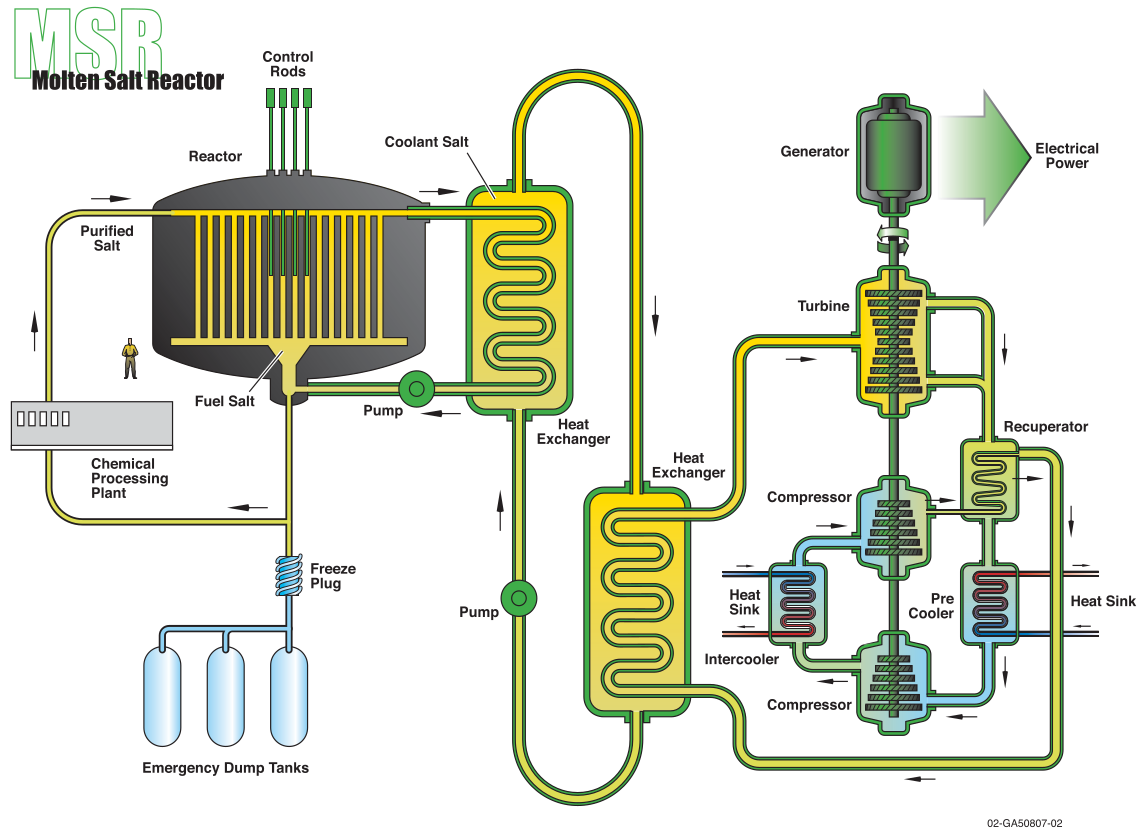
\includegraphics[width=.7\columnwidth]{msr}
	\caption{Schematic diagram of the \gls{MSR} concept. Retrieved from
	\cite{u.s._doe_nuclear_energy_research_advisory_committee_technology_2002}.}
	\label{fig:msr}
\end{figure}

The \gls{MSR} is one of six advanced reactor concepts selected for improved safety, sustainability,
efficiency, and cost over the current generation of predominantly \glspl{LWR} at the \gls{GIF}
\cite{u.s._doe_nuclear_energy_research_advisory_committee_technology_2002}.
Due to the large fuel expansion coefficient, \glspl{MSR} possess an inherently robust
safety feature in the strong negative fuel temperature coefficient of
reactivity \cite{elsheikh_safety_2013}. This reactivity coefficient limits the
maximum temperature that the reactor core would experience in particular accident
scenarios, such as an unprotected reactivity insertion, because the subsequent
rise in core temperatures induces a significant drop in reactivity,
quickly neutralizing the initial reactivity insertion. \glspl{MSR} also
operate at a large thermal margin to boiling and can rely on natural
circulation in the event of a pump failure. For an additional layer of safety, many \gls{MSR}
designs incorporate a drain plug made of actively-cooled frozen salt, which
melts when the core temperatures exceed safety thresholds. Hot molten salt
in the core would then flow into a drain tank designed to hold the fuel salt in
a subcritical configuration to disrupt any further chain fission reactions.

Some \glspl{MSR}, like the \gls{MSBR} or the \gls{MSFR}, can
incorporate the thorium fuel cycle for improved sustainability arising from the
use of abundant natural thorium resources and reduced transuranic waste
\cite{heuer_towards_2014}. The latter consequence also reduces costs
associated with long-term nuclear waste storage. Online fuel reprocessing raises the capacity
factor by reducing reactor downtime during reactor operation \cite{dolan_1_2017}.
Molten salt coolant loops can operate at near atmospheric pressures which eliminates the need for a
thick pressure vessel and drives down construction costs. We can make further economic arguments
supporting \glspl{MSR} in the context of the
carbon-constrained future envisioned in the \gls{IEA}'s \gls{NZE} roadmap
\cite{iea_net_2021}. The roadmap for minimizing carbon emissions requires solar photovoltaic- and
wind-dominated energy markets, which can results in highly variable and non-dispatchable
electricity generation. The resulting volatility in electricity prices
encourages the construction of heat storage and peak power
production plants. At the same time, demand for carbon-neutral
fuel will rise as electrification is economically unfeasible
for some industries, such as the aviation and marine sectors, which depend on
energy-dense fuels for propulsion.
The most cost-efficient options for heat storage, peak power production, and carbon-neutral fuel
production all require high-temperature heat \cite{forsberg_market_2020}.
This requirement favors \glspl{MSR}, which can deliver heat at higher average
temperatures than \glspl{LWR} and \glspl{SFR}.

Significant hurdles still stand in the way of commercial \gls{MSR} deployment \cite{dolan_27_2017}.
Major technological challenges include the need for further research on \gls{MSR} safety analysis,
irradiation and corrosion behavior of \gls{MSR} structural components, fission product tracking
and processing, \gls{MSR} nuclear safeguards measures, and the development of \gls{MSR} hydraulic
and heat exchanger components.

\subsection{Past \& Present \gls{MSR} Research \& Development}

\gls{ORNL} researchers first conceived the \gls{MSR} concept in pursuit of a high-temperature
liquid fuel reactor for the US Aircraft Nuclear Propulsion program in
the 1950s \cite{rosenthal_molten-salt_1970}. They
built the first ever operational \gls{MSR}, the 2.5 MW$_{\text{th}}$
\gls{ARE} reactor at \gls{ORNL}. The successful demonstration of the \gls{ARE} spurred further
research into adapting \glspl{MSR} for civilian power generation \cite{rosenthal_molten-salt_1970}.
Continued \gls{MSR} research efforts culminated in designing constructing, and successfully
operating of the 8-MW$_{\text{th}}$, thermal-spectrum \gls{MSRE} with
graphite channels and a LiF-BeF$_2$-ZrF$_4$-UF$_4$ fuel salt mixture
\cite{haubenreich_experience_1970}. In addition to other operational achievements, the
\gls{MSRE} became the first reactor to run on $^{233}$U fuel bred from $^{232}$Th. Building on
their experience with the \gls{MSRE}, \gls{ORNL} proposed a new program for constructing and
operating a demonstration reactor based on the \gls{MSBR} concept
\cite{macpherson_molten_1985}. The \gls{MSBR} is a thermal-spectrum \gls{MSR} with fertile
$^{232}$Th isotopes mixed directly into the \gls{FLiBe} molten salt for $^{233}$U breeding. The
\gls{MSBR} was to rely on continuous online reprocessing to add fertile
material and remove fission product neutron poisons.
However, the \gls{MSBR} project was canceled prior to the demonstration stage in
favor of the \gls{LMFBR}, which had benefited from a longer development time and more substantial
political backing \cite{macpherson_molten_1985}.

Following a relative lull lasting until the late 1990s, renewed research efforts and interest from
the \gls{GIF}
provided new impetus for \gls{MSR} research and development. As of the end of 2024, numerous
\gls{MSR} designs exist at various stages of development. Leading \gls{MSR} designs, in terms of
development, licensing, or demonstration, include the \gls{MSFR} \cite{merle_optimized_2007},
\gls{MCFR} \cite{terrapower_terrapower_2021}, TMSR-LF1 \cite{zhang_review_2018}, and \gls{IMSR}
\cite{leblanc_18_2017}. The \gls{MSFR} is a fast-spectrum breeder reactor developed through
collaboration among European institutes with funding support from the
European Union. Figure \ref{fig:msfr} shows a schematic diagram of the \gls{MSFR}. As opposed to
the multi-channel design of the \gls{MSRE} and \gls{MSBR}, the \gls{MSFR} is a pool-type design and
the reactor core consists of a large molten salt pool without graphite moderators to avoid
frequent graphite replacements and positive graphite temperature reactivity feedback. The
\gls{MCFR} is a similar pool-type reactor under active development at TerraPower. TerraPower and
Southern Company embarked on a joint project to design, construct, and operate a prototype
\gls{MCRE} design with funding support from the \gls{DOE}'s \gls{ARDP}. \gls{CAS} launched the
\gls{TMSR} program in 2011 to develop and construct both solid-fueled and liquid-fueled \gls{TMSR}
designs \cite{zou_research_2019}. They finished construction of TMSR-LF1, a 2-MW$_{\text{th}}$
liquid-fueled prototype, in August 2021 and received approval for reactor commissioning in August
2022. Lastly, Canada-based Terrestrial Energy is also developing its \gls{IMSR}, a small modular
\gls{MSR} based on the \gls{MSRE}. It passed a joint technical review by
Canadian and US nuclear regulators in July 2022.

Developing \gls{MSR} simulation software plays a vital role in supporting \gls{MSR}
development. Accurate reactor modeling capabilities
accelerate reactor design and optimization by enabling quicker iteration through numerous design
changes. \gls{MSR} simulation software are also essential tools in reactor safety analysis and
licensing efforts since reactor developers must demonstrate and verify that the \gls{MSR} systems
perform as designed and remain safe under various accident scenarios. 
%
\begin{figure}[htb!]
	\centering
	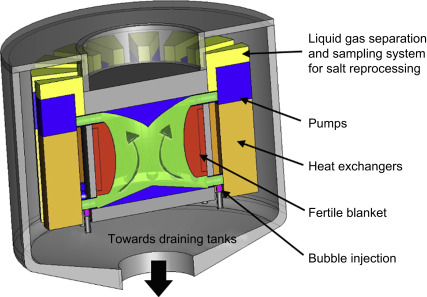
\includegraphics[width=.7\columnwidth]{msfr}
	\caption{Schematic diagram of the \gls{MSFR}. Retrieved from 
	\cite{allibert_7_2016}.}
	\label{fig:msfr}
\end{figure}

\subsection{Challenges in Multiphysics \gls{MSR} Modeling \& Simulation}

While modeling \glspl{MSR} is not necessarily more difficult than modeling
solid-fueled reactors, we must adapt our software tools to accurately model the
unique phenomena found in these circulating-fuel reactors. The differences in
the challenges of simulating \glspl{MSR} compared to solid-fueled reactors stem
primarily from the liquid fuel form of the fuel salt \cite{diamond_phenomena_2018,
huff_identifying_2019}.

Liquids generally exhibit greater thermal expansion per unit increase in temperature than solids.
The decreased fuel salt density due to thermal expansion
increases the likelihood of neutrons escaping the fuel region
and being absorbed by non-fissile material elsewhere in the reactor.
Consequently, combined with the temperature-dependent Doppler broadening of
resonance capture cross sections, \glspl{MSR} possess stronger negative fuel
temperature reactivity feedback than their solid-fueled counterparts
\cite{elsheikh_safety_2013}. These
phenomena ultimately result in strong interactions between the neutron fluxes
and the fuel salt temperatures, given that neutron fluxes affect fuel salt temperatures
through fission heat generation and fuel salt temperatures affect neutron
fluxes through the mechanisms described previously.

With the fuel salt also providing cooling in the core through advective heat
transfer, velocity flow
profiles in the fuel salts strongly impact the temperature distribution via
advection-dominated heat transfer \cite{diamond_phenomena_2018}. The flow-driven
temperature distribution contrasts
with the relatively static temperature profiles in fuel pins and
other solid fuel types, which are physically separate from the coolant.

\Glspl{DNP} flow freely within the primary coolant loop instead of
being held in place as in solid-fueled reactors. Thus, the delayed neutron
source distribution varies significantly depending on the flow profile and
velocity of the salt. In addition, the reactor loses some delayed neutrons from out-of-core
\gls{DNP} decay. These delayed neutrons are considered lost as they are emitted
in subcritical regions and are unlikely to contribute to further fission
reactions in the active core. The reduced delayed neutron fraction in the core
contributes to a greater prompt power spike following a reactivity insertion
event than solid-fueled reactors, absent any temperature reactivity
feedback.

Molten-salt flow along various parts of the coolant loop may fall within the turbulent flow
regime, characterized by chaotic eddies, vortices, and other flow instabilities.
Turbulent flow effects further complicate multiphysics interactions of flow with the temperature
and \gls{DNP} distribution. Turbulent flow effects contribute significantly to advection-dominated
heat and particle transfer in molten salt systems, thereby causing enhanced mixing. Therefore,
multiphysics software for \gls{MSR} analysis require adequate flow modeling capabilities with
support for \gls{DNP} drift and some form of turbulence modeling.

\gls{MSR} simulation tools require transient modeling capabilities to simulate transient
accident scenarios. Furthermore, several transient scenarios involve control rods, either as active
safety mechanisms or as accident initiators through unintended control rod ejection. Therefore,
\gls{MSR} simulation tools also require accurate control rod modeling capabilities to run
numerical analyses of accident scenarios involving control rods.

\subsection{Moltres for Multiphysics \gls{MSR} Analysis}

Moltres \cite{lindsay_moltres_2017} is an open-source multiphysics reactor simulation software
explicitly developed considering \gls{MSR} characteristics in mind. Moltres is
built on the \gls{MOOSE} \cite{giudicelli_30_2024} open-source finite-element framework,
which facilitates multiphysics coupling between different
\gls{MOOSE}-based and \gls{MOOSE}-wrapped applications. The \gls{MOOSE} framework also provides
Moltres with advanced meshing and numerical solver capabilities through interfacing with libMesh
\cite{kirk_libmesh_2006} and PETSc \cite{satish_petsc_2019} open-source libraries. Therefore,
Moltres supports up to 3-D unstructured meshes, scales well on high-performance computing systems,
and provides a flexible multiphysics coupling system, which can be tailored for different types of
simulations.

Moltres models coupled neutronics and thermal-hydraulics in reactors. While
generally applicable to most reactor concepts, much of
Moltres' development focuses on meeting the needs of \gls{MSR} multiphysics simulations.
Together with \gls{MOOSE}'s \texttt{Heat}
\texttt{Conduction} and \texttt{Navier-Stokes} \cite{peterson_overview_2018}
modules, Moltres solves the multigroup neutron diffusion
equations for an arbitrary number of energy and precursor groups and
thermal-hydraulics equations simultaneously on the same mesh (or separately solved and coupled
through fixed-point iterations if desired).

Lindsay et al. \cite{lindsay_introduction_2018}
demonstrated Moltres' multiphysics \gls{MSR} modeling capabilities with 1-D salt
flow modeling in axisymmetric and 3-D models of the \gls{MSRE}. The neutron flux and
temperature distributions agreed qualitatively with legacy
\gls{MSRE} data albeit with some minor quantitative discrepancies due to
simplifications and assumptions in the reactor geometry. I demonstrated Moltres' capabilities for
1) looping of \gls{DNP} drift back into the reactor core, 2) coupling the \gls{DNP}
drift to numerically calculated salt flow profiles within the reactor core,
and 3) a decay heat model to simulate decay heat from fission products, with a 2-D axisymmetric
design of the \gls{MSFR} in my Master's thesis \cite{park_advancement_2020}.

While the Moltres
model of the \gls{MSFR} showed good agreement with other studies in most steady-state and transient
simulation cases, the Moltres model showed significant discrepancies during pump-initiated
transient scenarios without a proper turbulence model. Instead, the model applied a
uniform eddy viscosity assumption, which proved inadequate under non-steady flow. In order to
advance Moltres as a multiphysics simulation software for \gls{MSR} analysis, Moltres requires a
turbulence modeling capability to capture adequate turbulent flow phenomena and their interactions
with other physics present in \glspl{MSR}. Of the various classes of turbulence models, a
\gls{RANS}-based model is most suitable for coupling with Moltres when considering computational
efficiency. The \gls{RANS}-based equations are time-averaged fluid flow equations
derived by separating the flow variable into its time-averaged and fluctuating components.
\gls{RANS}-based models are also well-validated, representing the most widely used turbulence
models for engineering applications.

In addition to new features, Moltres would benefit from further \gls{VV} of its existing
multiphysics capabilities to identify software bugs and ensure reliable results. Accurate modeling
and simulation of salt flow-induced \gls{DNP} drift and the strong coupling between neutronics and
thermal-hydraulics are crucial for \gls{MSR} simulation tools.
% Therefore, the proposed work will include relevant \gls{VV} studies for Moltres.

\subsection{Control Rod Modeling in \glspl{MSR}}

While some \gls{MSR} concepts completely eliminated control rods from their signs, many still
retain them. Control rods consist of strong
neutron absorbers like boron, cadmium, or gadolinium to absorb and thus reduce the number of
neutrons available to contribute to further fission chain reactions. All reactors start operation
with excess reactivity to ensure enough fissile material is available to maintain power operation
and last through to the next scheduled refueling. Control rods and burnable poisons balance the
initial excess reactivity. Control rods are also helpful
for ramping the power up or down during start-up, shut-down, or load-following operations. Most
importantly, control rods provide a safety mechanism for quickly shutting down a reactor under
dangerous conditions. Rapid control rod insertion is the primary mechanism of a reactor scram to
reliably introduce a large negative reactivity insertion in response to an unintended reactivity
insertion or other events that may threaten the reactor's safe operation. 

Amongst other tasks in reactor modeling, reactor physics analysts aim to accurately reproduce
control rod worth, which is measured as the relative reduction
in the neutron multiplication factor $k_\text{eff}$ due to the insertion of the control rod in the
reactor. They are also interested in the accompanying change in flux shape near the
control rod. Neutrons entering the control rods are more likely to be absorbed than
adjacent regions in the reactor core. Therefore, control rods induce highly anisotropic neutron
angular fluxes and sharp gradients in the neutron flux in their vicinity. Control rods also cause
shifts in the neutron energy spectrum because their absorption cross sections are much higher in
the lower neutron energy range; more energetic neutrons generally have a higher probability of
escaping the control rod region. As a consequence, modeling control rods accurately requires
high-fidelity computational methods to capture the angular dependence in the neutron
flux near the highly absorbing medium. Existing reactor analysis workflows often rely on Monte
Carlo methods for high-fidelity neutron transport calculations.

However, traditional neutron transport methods, including Monte Carlo methods, are computationally expensive
and thus are mainly used for time-independent neutronic analyses. For solid-fueled reactors,
static control rod analyses can be justified due to the relatively static temperature distribution
shape in the fuel and disparate timescales of heat transfer from the fuel to
the coolant (seconds) and neutron flux changes (microseconds to milliseconds). In
\glspl{MSR}, this distinction blurs due to molten salt serving the dual role of fuel and
coolant and the strong fuel temperature reactivity feedback. For time-dependent multiphysics
simulations coupling neutronics to \gls{TH} and other physics present in nuclear reactors, most
reactor analyses rely on neutron diffusion theory for modeling neutronics. The issue with applying
neutron diffusion theory near control rods arises because neutron diffusion theory approximates
neutron transport theory by integrating over the angular variables. As a result, diffusion-based
methods perform poorly in reactor systems with control rods.

% To tackle the issue of modeling control rods in \glspl{MSR} with the multigroup neutron diffusion
% solver in Moltres, I will develop and implement a novel hybrid method for incorporating neutron
% transport-derived corrections to the neutron diffusion method while largely preserving the
% computational efficiency of the neutron diffusion method over neutron transport methods. This will
% allow for computationally feasible transient analysis of \glspl{MSR} that incorporate thermal and
% neutronic feedback on variable timescales.

\section{Research Objectives and Outline}

The overarching goal of this work is to improve on Moltres as a reliable, intermediate-fidelity
simulation tool for multiphysics \gls{MSR} analysis that can be run on workstations as well as on
large leadership-class computing clusters. Thus, new and existing capabilities in Moltres must
be accurate within accepted bounds, rigorously verified, computationally efficient, and highly
scalable. These conditions form the underlying development principles of this work.

The scope of this dissertation can be divided into two main objectives.
%
%\begin{enumerate}[itemindent=20pt, listparindent=1.5em, label=\textbf{\arabic*}]
%  \item \textbf{Verification and validation of multiphysics capabilities in
%    Moltres}

    The first objective is to verify and validate multiphysics capabilities in Moltres for
    modeling and simulating
    the strong interactions between the neutronics and thermal-hydraulics in \glspl{MSR}. This
    will be accomplished through two separate studies: verifying Moltres against the CNRS
    benchmark \cite{tiberga_results_2020} for fast-spectrum \gls{MSR} analysis, and modeling the
    \gls{MSRE} zero-power pump start-up and coast-down experiments. I will perform the second study
    in collaboration with the developer of QuasiMolto \cite{reynolds_analysis_2023} as a \gls{VV}
    study.
%    with the additional aim of creating a reproducible numerical benchmark of the listed
%    \gls{MSRE} experiments.
%
%  \item \textbf{Implementation and verification of a \gls{RANS}-based turbulence model in Moltres}
    This objective includes implementing and verifying a Spalart-Allmaras turbulence model in
    Moltres to support future turbulent flow
    simulations for \gls{MSR} analyses. This will address the absence of turbulence modeling
    capability in Moltres and the consequent restriction on Moltres for modeling \gls{MSR} systems
    with complex turbulent flow.

%  \item \textbf{Development of a novel hybrid $S_N$-diffusion method for improved control rod modeling in Moltres}

    The second objective is to develop, implement, and demonstrate a novel hybrid $S_N$-diffusion
    method for accurate control rod modeling in
    time-dependent \gls{MSR} analyses. The hybrid method uses the discrete ordinates ($S_N$)
    neutron transport method to generate transport corrections in regions near control rods for
    drift correction terms in modified neutron diffusion equations. The $S_N$ method is applied on
    a reduced problem domain to ensure the hybrid method remains tractable on small to moderate
    computing clusters.
%\end{enumerate}

Chapter 2 presents a literature review of existing multiphysics \gls{MSR} simulation software,
\gls{VV} studies on \gls{MSR} modeling and simulation, turbulence modeling in \gls{MSR} systems,
and transport-correction techniques for neutron diffusion methods.
Chapter 3 provides an in-depth description of Moltres and its existing capabilities in the context
of previously published work. This chapter then presents Moltres \gls{VV} results for the CNRS
benchmark and the numerical \gls{MSRE} zero-power pump experiment studies. Following these studies,
the chapter presents the implementation and verification of the Spalart-Allmaras turbulence model
in Moltres.
Chapter 4 presents the theory and numerical implementation of the hybrid
$S_N$-diffusion method in Moltres. These include the $S_N$ method implementation, the transport
correction formulations, the iteration algorithm, the $S_N$-diffusion coupling implementation, and
general implementation details relating to the underlying numerical solver in Moltres.
Chapter 5 presents the verification and demonstration of the hybrid $S_N$-diffusion method for
$k_\text{eff}$ and rod worth calculations through
$k$-eigenvalue simulations of 1-D, 2-D, and 3-D \gls{MSRE} models. The hybrid method is verified
against reference results from OpenMC Monte Carlo neutron transport code and \gls{MSRE}
experimental data.
%Chapter 6 presents the demonstration of the hybrid $S_N$-diffusion method in time-dependent
%reactivity-initiated simulations modeling the \gls{MSRE} rod drop and reactivity insertion
%experiments.
Chapter 6 presents a demonstration of the hybrid $S_N$-diffusion method in a time-dependent
reactivity-initiated simulation modeling a \gls{MSRE} rod drop experiment.
Chapter 7 concludes this dissertation by summarizing the results presented, identifying limitations
in this work, and providing potential research directions to address those limitations or extend
this work.

%\glsresetall

\chapter{Molten Salt Reactor Modeling and Simulation}
\label{chap:lit}
\glspl{MSR} possess unique characteristics which render existing \gls{LWR}
analysis software inappropriate for \gls{MSR} analysis. Legacy \gls{LWR}
software typically scale poorly on modern high-performance computing
clusters and do not support complex geometries beyond the regular square or hexagonal shapes of
\gls{LWR} fuel assembly lattices. Furthermore, \glspl{MSR} feature strong coupling between the
neutronic and thermal-hydraulics physics, forcing segregated solvers into taking smaller timesteps
to maintain solver accuracy and stability. This chapter presents a literature
review of existing multiphysics simulation software developed for \gls{MSR}
analysis. This work focuses on software for analyzing short-term reactor
dynamics, which requires accurately simulating various transient
scenarios such as reactor start-up and coast-down, load-following operations,
steady-state operation, and accident analysis. Long-term dynamics such as fuel
burnup and structural corrosion fall outside the scope of this work.
This chapter also provides a literature review of turbulence modeling and transport-correction
techniques for the neutron diffusion method relevant to control rod modeling.

\section{MSR Multiphysics Modeling} \label{sec:msr-multiphysics}

The existence of multiple, disparate physics in a single system constitutes a multiphysics system.
Consequently, we need multiphysics software to accurately model a multiphysics system. Employing
well-verified single-physics software for coupled multiphysics simulations does not guarantee
stability, accuracy, or robustness \cite{keyes_multiphysics_2013}. Nevertheless, coupling separate
single-physics software for multiphysics simulations is a viable and popular option with proper
implementation. With strong coupling between different physics, extra care must be
taken to capture various multiphysics interactions accurately. For instance, the strong coupling
between neutron flux and temperature in \glspl{MSR} in \glspl{MSR} necessitates robust coupling
techniques. Na\"ive multiphysics coupling algorithms may result in longer computation times
at best and a lack of convergence in simulations at worst.

Whether one couples separate single-physics software together or develops a multiphysics software
under a single numerical solver framework, multiphysics software for modeling \glspl{MSR} must
employ \textit{tight coupling schemes} to couple the neutronics and thermal-hydraulics governing
equations to capture the strong multiphysics interactions in transient \gls{MSR} simulations
accurately without resorting to very small time-steps \cite{aufiero_development_2014}. Tightly
coupled numerical models handle multiphysics interactions by either updating all state
variables simultaneously in one monolithic solve (\textit{full coupling}) or
iteratively updating all state variables (\textit{fixed point iterations})
until the solution converges in every timestep \cite{keyes_multiphysics_2013}.
Full coupling tends to be more computationally expensive because it combines
all physics equations into a single large system of equations to be solved
simultaneously. In contrast, fixed point iterations involve operator splitting to
separate the system of equations into smaller systems based on their associated
physics, solving smaller systems separately, and iteratively updating the state
variables until convergence. Fixed point iterative methods can be less
stable, less accurate, and have poorer
convergence rates since these methods make iterative corrections
without regard to potentially destabilizing modes introduced by the
multiphysics coupling \cite{keyes_multiphysics_2013}. In particular, Lindsay et al.\
\cite{lindsay_introduction_2018} demonstrated the non-convergence of a multiphysics \gls{MSR}
model without delayed neutron precursors when using fixed point iterations. While fully coupled
schemes result in large systems of equations to solve, they can still outperform fixed point
iterative methods in some multiphysics problems through superior stability and convergence rates.
Conversely, proven techniques exist for improving the performance of fixed point iteration coupling
schemes for many relevant computational multiphysics research fields, including reactor analysis
\cite{ragusa_consistent_2009}. Fixed point iterative methods also allow for different temporal and
spatial discretization schemes to meet the requisite resolution of each
individual physics model.

In contrast to tight coupling schemes, \textit{loose coupling schemes}
solve each set of single-physics equations using state variable
data from the previous timestep without iterative corrections within every
timestep. Loosely coupled schemes are inappropriate for modeling \glspl{MSR},
given the strong coupling between neutronics and thermal-hydraulics.
Aufiero et al.\ \cite{aufiero_development_2014} demonstrated a loose coupling
approach that failed to reproduce the expected increase in reactor power
in an \gls{MSR} in response to a 150 pcm reactivity insertion. One rare use case for loose
coupling is pseudo-transient problems for converging a multiphysics system to steady state.

Consequently, MSR multiphysics simulation tools must employ, at the very least, tight coupling
schemes through fixed-point iterations for most applications. The optimal coupling scheme depends
on the multiphysics model and the underlying numerical solver implementations.
The next subsection reviews existing \gls{MSR} multiphysics software and their applications.

\subsection{Review of MSR Multiphysics Simulations and Results} \label{sec:msr-tools}

Several simulation tools have been developed for \gls{MSR} modeling in the last two decades. Given
the focus on developing high-fidelity \gls{MSR} software to support reactor design optimization,
this literature review omits coupled neutronics/thermal-hydraulics MSR simulation work with
zero-dimensional point reactor kinetics in favor of those with spatially-resolved neutronics
methods.

\subsubsection{Coupling Existing Single-Physics Codes for MSR Modeling}

Coupling single-physics software to form integrated multiphysics tools allows researchers to
leverage existing well-validated, single-physics software. These single-physics software are also
highly optimized for solving specific \glspl{PDE} relevant to the investigated system.
Many \gls{MSR} simulation tools employ tight coupling to couple separate neutronics and
thermal-hydraulics solvers.

In 2007, Krepel et al.\ \cite{krepel_dyn3d-msr_2007} extended the
\gls{LWR} nodal diffusion code DYN3D to account for \gls{DNP} drift and fission energy deposition
in the coolant for \gls{MSR} modeling. The extended DYN3D-MSR code also contains the FLOCAL
thermal-hydraulics model for coolant flow and conjugate heat transfer modeling. Their \gls{MSRE}
and \gls{MSBR} models consisted of homogeneous hexagonal nodes (mesh elements) for the nodal
diffusion calculation coupled to individual hexagonal unit cells comprising of graphite with
circular fuel channels in the center for the thermal-hydraulics calculations. They simulated
steady-state operation; start-up, coast-down, natural circulation transients; and an overcooling
transient in their \gls{MSRE} model. They also modeled steady-state operation and a single-channel
blockage transient in their \gls{MSBR} model.

At the \gls{TUD}, Kophazi et al.\
\cite{kophazi_development_2009} coupled their in-house 3-D neutron diffusion software DALTON
\cite{boer_validation_2010} and thermal-hydraulics
software THERM to develop a 3-D \gls{MSR} simulation tool. They homogenized the heterogeneous fuel
and graphite region of the \gls{MSRE} for the neutronics calculation. They discretized the
homogeneous region into a Cartesian mesh and modeled a more accurate representation of the oblong
fuel channels in the graphite core matrix instead of the circular shape by Krepel et al.\
\cite{krepel_dyn3d-msr_2007}.

Both efforts by Krepel et al.\ and Kophazi et al.\ showed good
agreement with \gls{MSRE} experimental data in their respective validation tests.
The researchers from \gls{TUD} continued in their approach of coupling separate single-physics
software to create \gls{MSR} simulation tools, as noted by the DALTON-HEAT
\cite{de_zwaan_static_2007} coupling to model the \gls{MSFR} \cite{fiorina_modelling_2014}. The
fast-spectrum \gls{MSFR} features a large pool of fuel salt in its single-channel design instead of
the \gls{MSRE}'s multi-channel design. As a result, the authors had to incorporate
multidimensional turbulent flow modeling to accurately model the complex flow profiles and
turbulence effects in the \gls{MSFR} during steady-state operation and transient scenarios. In a
later effort from the same institute, Tiberga et al.\ \cite{tiberga_discontinuous_2019} coupled
PHANTOM-$S_N$ and DGFlows for their participation in the CNRS benchmark study
\cite{tiberga_results_2020}. Developed at the \gls{CNRS}, the CNRS benchmark facilitates
code-to-code verification of \gls{MSR} multiphysics software \cite{aufiero_testing_2018}. Tiberga
et al.\ showed that their coupled PHANTOM-$S_N$/DGFlows software was consistent with
OpenFOAM-based \gls{MSR} simulation tools. Further details on their study and the CNRS benchmark
is available in Section \ref{sec:msr-vv}.

Another multiphysics package was developed at the \gls{PSI} by coupling the \gls{LWR}
thermal-hydraulics system software \gls{TRACE} \cite{nrc_trace_2007}
with the nodal neutron diffusion software \gls{PARCS} \cite{downar_parcs_2010} for safety
analysis of the \gls{MSFR} \cite{pettersen_coupled_2016}. The right circular cylinder \gls{MSFR}
design was approximated using hexagonal nodes in \gls{PARCS} while \gls{TRACE} simulated
Reynolds-averaged, inviscid coolant flow. While modeling inviscid flow reduces computational costs
by eliminating the need for expensive turbulence modeling, this approach neglects turbulent flow
and turbulent mixing effects.

More recently, Jaradat et al.\ \cite{jaradat_development_2021}
extended the 3-D $P_1$ and $SP_3$ nodal transport code PROTEUS-NODAL to support \gls{DNP} drift.
Yang et al.\ \cite{yang_development_2022} then developed a coupled simulation tool of PROTEUS-NODAL
and \gls{SAM}. They modeled the \gls{MSFR} on a 2-D axisymmetric geometry
and the \gls{MSRE} on a 3-D R-$\theta$-Z geometry with twelve 1-D flow channels. The \gls{SAM} flow
model relied on the algebraic mixing length model for turbulence modeling. Both results
reproduced the expected trends observed in published experimental and simulation data. However,
their 1-D flow models neglected complex turbulent flows expected in the \gls{MSFR}.

With modern advancements in computing hardware and growing access to
high-performance computing systems, others have developed multiphysics tools by
coupling the \gls{CFD} software OpenFOAM
\cite{the_openfoam_foundation_ltd_openfoam_2021} with the Monte Carlo particle
transport software Serpent \cite{leppanen_serpent_2014}, thus achieving
high-fidelity neutronics calculations in transient reactor analyses \cite{laureau_transient_2017,
blanco_neutronic_2020}. To that end, Serpent has a multiphysics interface supporting coupling
with other physics software \cite{leppanen_development_2013}.

Laureau et al.\
\cite{laureau_transient_2017} developed a different technique called the
\gls{TFM} method by introducing additional time-dependence
operators to conventional fission matrices typically used to accelerate source
convergence in Monte Carlo neutronics calculations. The \gls{TFM} method
pre-calculates three \glspl{TFM} of the reactor system in Serpent. It
interpolates the matrix values during the actual transient calculations to
incorporate temperature-induced salt expansion and Doppler effects on the neutron cross sections
and, ultimately, the neutron flux. Laureau et al.\ opted to subcycle the neutronics calculations by
setting smaller timesteps than the thermal-hydraulics calculations
to take advantage of the differing physics timescales. They demonstrated load-following capability
and parametric studies of overcooling and reactivity insertion transients in the \gls{MSFR}.

Blanco \cite{blanco_neutronic_2020} took a more direct approach by
compiling Serpent as an internal \texttt{C}-based function within OpenFOAM's
\texttt{C++}-based framework. This approach reduced the amount of external data
transfers between Serpent and OpenFOAM as both software have access to shared
memory during runtime. Their integrated tool employs the Quasi-Static
method for transient neutronics calculations and runs Serpent Monte Carlo
calculations several times per timestep until convergence is reached.
Blanco demonstrated the Serpent-OpenFOAM tool on the CNRS benchmark specified by Tiberga et al.\
\cite{tiberga_results_2020}.

\subsubsection{Integrated Multiphysics Modeling Frameworks for MSR Modeling}

Another \gls{MSR} simulation approach involves developing inherently multiphysics software that
handle all multiphysics calculations and data transfer internally. Among earlier efforts, Nicolino
et al.\ \cite{nicolino_coupled_2008} and Zhang et al.\ \cite{zhang_development_2009} recognized the
need for more robust multiphysics coupling, acceleration techniques and internal data transfers
to reduce execution times. They each independently developed unnamed multiphysics simulation tools
and demonstrated their tools with non-moderated \gls{MSR} designs. Nicolino et al.\ presented one
of the first \gls{MSR} models with multi-dimensional flow, governed by the Navier-Stokes equation
with the Boussinesq approximation. They performed steady-state and transient calculations on a 2-D
axisymmetric model of the \gls{MOSART} reactor \cite{ignatiev_molten_2014}. Zhang et al.\ also
developed a similar 2-D axisymmetric solver, but they incorporated a $k$-$\epsilon$ turbulence
model and performed calculations on an unnamed pool-type \gls{MSR} design with graphite reflectors.
Both studies implemented the neutron diffusion model for neutronics modeling.
Later, Li et al.\ \cite{li_transient_2015} demonstrated the
steady-state and transient analysis capabilities of COUPLE, a neutronics and
thermal-hydraulics software, on a 2-D axisymmetric model of the \gls{MSFR}. COUPLE also solves the
neutron diffusion equations and the Navier-Stokes equations with the $k$-$\epsilon$ turbulence
model.

Others adopted extensible software frameworks for developing numerical solvers
to develop multiphysics reactor analysis software. Examples of these software
frameworks include the commercial COMSOL
Multiphysics\textsuperscript{\textregistered} software
\cite{comsol_ab_comsol_nodate}, the aforementioned open-source CFD toolbox
OpenFOAM, and the open-source finite-element
framework \gls{MOOSE} \cite{giudicelli_30_2024}. Researchers at
\gls{PoliMi} developed an \gls{MSR} simulation tool in COMSOL and
modeled the \gls{MSBR} as a single axisymmetric fuel channel with a uniform
flow profile \cite{cammi_multi-physics_2011}, followed by the \gls{MSRE} core
also as a single axisymmetric fuel channel with parabola-shaped laminar flow
\cite{cammi_dimensional_2012}. They later expanded on their approach by
modeling the \gls{MSRE} upper plenum, downcomer and lower plenum, primary heat
exchanger, and secondary heat exchanger as 0D systems (lumped-parameter model)
and substituting the 2-D fuel channel with a 3-D fuel channel which more closely
resembled the actual fuel channels in the \gls{MSRE}
\cite{zanetti_geometric_2015}. Other than the \gls{MSRE}, they also modeled the
\gls{MSFR} in a later publication \cite{fiorina_modelling_2014}, which also featured \gls{TUD}'s
DALTON-HEAT coupled multiphysics tool.

Other institutes have dedicated significant development work towards
OpenFOAM-based \gls{MSR} simulation tools. Aufiero et al.\
\cite{aufiero_development_2014} first introduced an OpenFOAM model developed
at \gls{PoliMi}. Their model implemented a neutron diffusion model and a
\gls{RANS}-based turbulence model under the incompressible flow assumption to demonstrate 2-D
and 3-D transient analyses of the \gls{MSFR}. Later advancements in the
\gls{PoliMi} solver include a fuel compressibility model with helium bubble
tracking to study fuel compressibility effects
\cite{cervi_development_2019} and an $SP_3$ neutron transport
model for improved neutronics calculations \cite{cervi_development_2019-1} in
the \gls{MSFR}. GeN-Foam is another OpenFOAM-based tool developed by Fiorina
et al.\ \cite{fiorina_gen-foam_2015} as a general reactor multiphysics solver
applicable to \glspl{MSR} and other reactor types. GeN-Foam features neutron
diffusion, $SP_3$, and $S_N$ neutronics models
\cite{fiorina_development_2016,fiorina_gen-foam_2015,fiorina_detailed_2019},
and thermo-mechanical modeling for reactor expansion effects. Using GeN-Foam,
Altahhan et al.\ \cite{altahhan_preliminary_2020} developed and optimized a
liquid-fuel \gls{MSR} design, while Shi \& Fratoni \cite{shi_gen-foam_2021}
simulated precursor drift effects in a homogenized \gls{MSRE} model. However, none of the
OpenFOAM-based tools have demonstrated the capability for time-dependent \gls{MSR} simulations
with explicit control rod modeling.

Finally, within the \gls{MOOSE} framework, simulation tools capable of modeling
\glspl{MSR} include Griffin \cite{abou-jaoude_coupled_2020}; and Moltres
\cite{lindsay_moltres_2017}\textemdash the subject of this work.
Griffin primarily tackles radiation transport problems, but the \gls{MOOSE}
framework facilitates multiphysics coupling with \gls{MOOSE}-based applications for other physics
such that all applications share the same data structure. This feature eliminates
computational costs from external data transfers and optionally allows for
\textit{fully coupled} calculations in which the application solves all physics
simultaneously. The mutual compatibility among different physics applications within the
\gls{MOOSE} framework simplifies the work required to couple
different physics solvers together to solve novel multiphysics problems. Similarly,
Moltres benefits from the highly-integrated cross-compatibility
within the ecosystem of \gls{MOOSE}-based applications. Abou-Jaoude et al.\
\cite{abou-jaoude_coupled_2020} coupled Griffin with Pronghorn, another
\gls{MOOSE}-based application for advanced reactor thermal-hydraulics modeling, to
demonstrate several steady-state \gls{MSR} simulation capabilities defined in
the CNRS benchmark. Lindsay et al.\
\cite{lindsay_introduction_2018} first demonstrated Moltres' \gls{MSR} modeling
capabilities on 2-D axisymmetric and 3-D Cartesian models of the \gls{MSRE} with
fixed velocity flow in a fully coupled neutronics and thermal-hydraulics simulations.
I later demonstrated some of Moltres' more recent developments through
modeling a 2-D axisymmetric model of the \gls{MSFR} for steady-state operation
and transient accident analysis \cite{park_advancement_2020}. The latter study
introduced looped \gls{DNP} flow, coupling the \gls{DNP} drift and temperature 
advection-diffusion to incompressible flow, and decay heat modeling
capabilities.

\subsection{MSR Multiphysics Modeling Verification \& Validation} \label{sec:msr-vv}

\Gls{VV} of simulation models are important components of simulation software development
\cite{sargent_verification_2010}. Verification involves checking whether a model's implementation
accurately represents the conceptual description and specifications. Model
validation is the process of checking whether a model is an accurate representation of the real
world within the range of its intended uses. For reactor software, model verification is commonly
performed by comparing them to other reactor software designed to run the same type of reactor
simulations. On the other hand, model validation is performed by comparing numerical results from
a simulation model to experimental data from the corresponding live test. The validity of a model
depends on the outcome of both model verification and validation.

The important multiphysics phenomena in \glspl{MSR} for model \gls{VV} are salt flow-induced
\gls{DNP} drift and the strong coupling between neutron flux and temperature advection-diffusion.
Delpech et al.\ \cite{delpech_benchmark_2003} published one of the first collaborative \gls{VV} work
for \gls{MSR} multiphysics modeling. Collaborators
from six institutions modeled \gls{MSRE} pump start-up, pump coast-down, and natural
circulation transients to assess and validate their models and codes for studying the effects of
salt flow on the reactivity and power. Given the wide range of neutronics methods, from
multidimensional Monte Carlo methods to zero-dimensional point reactor kinetics, some deviations
were observed between different codes. Nevertheless, all results generally agreed
with \gls{MSRE} experimental data from \gls{ORNL}.

As mentioned in Subsection \ref{sec:msr-tools}, Tiberga et al.\ \cite{tiberga_results_2020}
published the CNRS benchmark to verify \gls{MSR} simulation tools designed for
fast-spectrum \gls{MSR} modeling. In contrast with the multi-channel \gls{MSRE} and its derivative
designs, the CNRS benchmark has a 2 m$\times$2 m problem domain of homogeneous fuel salt mimicking
the large salt pool in fast-spectrum \gls{MSR} designs. The CNRS benchmark consists of three
phases: single-physics calculations in Phase 0, problems that gradually
introduce multiphysics coupling in Phase 1, and time-dependent perturbation problems in Phase
2. Thus, the benchmark provides a systematic approach to help code developers
identify sources of discrepancies that may otherwise be masked by error cancellation or other
dominant sources of discrepancies. The final steady-state and time-dependent problems involve
studying the effects of natural circulation and lid-driven flow on the reactivity and power output.
Aside from the problem specifications, Tiberga et al.\ also published the associated group
constant cross section data required by deterministic neutronics solvers to perform neutronics
calculations. Four institutions participated in the benchmarking exercise with neutron diffusion,
$SP_N$, and $S_N$-based solvers for the neutronics calculations. Their measured neutronics and
\gls{TH} parameters showed excellent agreement within up to 2.5\% discrepancy from their combined
average.

Neutronic benchmark studies of the \gls{MSRE} and the \gls{MSFR} by Fratoni et al.\
\cite{fratoni_molten_2020} and Brovchenko et al.\ \cite{brovchenko_neutronic_2019} measured the
delayed neutron losses due to the decay of \glspl{DNP} flowing out of the active core region.
Fratoni et al.\ sought to establish a standard validation platform for \gls{MSR} neutronics
simulation tools with \gls{MSRE} experimental data for inclusion in the \gls{IRPhEP} handbook.
They characterized and validated a model of the \gls{MSRE} in the Monte Carlo particle transport
code Serpent. The \gls{MSFR} neutronics benchmark by Brovchenko et al.\ featured results
from multiple \gls{MSR} simulation tools by several collaborators. Their assessment found that
the choice of nuclear database for the cross sections and decay data has the most significant
impact on the neutronics results.

While these publications have addressed significant technical gaps, there is room to develop
further \gls{VV} benchmarks for multiphysics \gls{MSR} modeling. For instance, the CNRS benchmark
does not assess the loss of delayed neutrons due to the decay of \glspl{DNP} flowing out of the
active core region. This phenomenon is important as the delayed neutron fraction in the core
directly impacts the transient power response in unprotected accident scenarios. Meanwhile, the
neutronic benchmark studies by Fratoni et al.\ \cite{fratoni_molten_2020} and Brovchenko et al.\
\cite{brovchenko_neutronic_2019} did not provide the standardized group constant data required by
most deterministic multiphysics \gls{MSR} simulation tools. Therefore, it is challenging to isolate
discrepancies arising from code implementations instead of discrepancies from using different
nuclear databases or stochastic uncertainties in Monte Carlo simulations. A suitable model
verification procedure for delayed neutron loss should ideally provide well-defined problems and
the necessary input data. It is also helpful to perform model verification studies on simpler
problems like the bare homogeneous problem domain in the CNRS benchmark before embarking on more
detailed validation studies that require accurate models of experimental setups.

\section{Turbulence Modeling in MSRs} \label{sec:lit-turb}

In fluid dynamics, turbulent flow is characterized by unsteady, irregular, and
chaotic fluid motion as opposed to neat, parallel flow layers in laminar flow
\cite{pope_turbulent_2000}. The transition from laminar to turbulent flow
typically occurs at Reynolds numbers between 2000 and 4000, depending on the
system \cite{pope_turbulent_2000}. Turbulent flows are expected in \glspl{MSR}.
Kedl \cite{kedl_fluid_1970} reports expected Reynolds numbers in the \gls{MSRE}
ranging from 1000 in the regular fuel coolant channels to over 10000 in the
flow distributor volute and core wall cooling annulus regions. For the
\gls{MSFR}, salt flow in the central core region is highly turbulent and
reaches Reynolds numbers on the order of $10^5$.

\subsection{Turbulence Models}

Numerous types of turbulence models exist for various turbulent flow
applications. The most common turbulence models can be classified into the
following categories by order of increasing fidelity and computational complexity:
%
\begin{itemize}
    \item \gls{RANS}-based models
    \begin{itemize}
        \item Eddy viscosity models
        \begin{itemize}
            \item Algebraic models
            \item One- and two-equation models
        \end{itemize}
        \item \gls{RSM}
    \end{itemize}
    \item \gls{DES}
    \item \gls{LES}
    \item \gls{DNS}
\end{itemize}

\gls{RANS}-based models are based on the \gls{RANS} equations obtained from
applying time-averaging to the fluid flow equations. The \gls{RANS}
equations separate flow into time-averaged $U$ and fluctuating $u$ components
and can be written in Einstein notation and Cartesian coordinates as:
%
\begin{align}
    \frac{\partial U_i}{\partial t} + U_j \frac{\partial u_i}{\partial x_j} =&
    -\frac{1}{\rho} \frac{\partial P}{\partial x_i} + \nu \nabla^2 U_i -
    \frac{\partial \langle u_i u_j \rangle}{x_j}
    \shortintertext{where}
    \langle \cdot \rangle =& \mbox{ time-averaging operator,} \nonumber \\
    \rho =& \mbox{ fluid density,} \nonumber \\
    P =& \mbox{ time-averaged pressure field,} \nonumber \\
    \nu =& \mbox{ kinematic viscosity.} \nonumber
\end{align}

Eddy viscosity models, which comprise the most widely used turbulence models
in use today \cite{rodi_turbulence_2017}, operate on the eddy viscosity
hypothesis which states that the Reynolds stresses in the \gls{RANS} equations
are given by:
%
\begin{align}
    \langle u_iu_j \rangle =& \frac{2}{3}k \delta_{ij} - \nu_T \left(
    \frac{\partial U_i}{\partial x_j} + \frac{\partial U_j}{\partial x_i}
    \right)
    \shortintertext{where}
    k =& \mbox{ mean turbulent kinetic energy,} \nonumber \\
    \delta_{ij} =& \mbox{ Kronecker delta,} \nonumber \\
    \nu_T =& \mbox{ eddy viscosity.} \nonumber \\
\end{align}

The various eddy viscosity models mainly differ in their approach to
the closure problem of calculating the eddy viscosity. As the name suggests,
algebraic models rely on algebraic equations to directly calculate the eddy viscosity
distribution from flow variables. As a result, algebraic models are
the least computationally intensive models for turbulence. Algebraic models
can be further categorized into uniform eddy viscosity models
and mixing length models. Uniform eddy viscosity models apply a uniform eddy
viscosity throughout the problem domain. The uniform eddy viscosity is
calculated from flow parameters such as the characteristic velocity, the
characteristic flow width, and empirically determined turbulent Reynolds
number.

Given that eddy viscosities usually vary significantly in most types of
flow, uniform eddy viscosity models have a limited range of applicability
\cite{pope_turbulent_2000}. Mixing length models add a level of complexity by
relating the eddy viscosity to spatially-varying flow parameters such as the
mean velocity gradient (Prandtl \cite{prandtl_7_1925} and Cebeci-Smith
\cite{smith_numerical_1967} models) or the mean rate of strain (Baldwin-Lomax
\cite{baldwin_thin-layer_1978} model) and an empirical mixing length parameter.
Combined with empirical data for the mixing length parameter, these
models provide better approximations of free shear flows but still
underperform for more complex flows involving flow separation and significant streamline curvature.

One- and two-equation turbulence models introduce differential equations to
describe turbulence quantities such as the turbulence kinetic energy and the
turbulence rate of dissipation to obtain the eddy viscosity distribution. The
most common and best-performing one-equation model is the Spalart-Allmaras
model, which directly provides an equation for the eddy viscosity with several
closure coefficients and functions \cite{wilcox_turbulence_2006}. The
Spalart-Allmaras model is considered ``complete'' as it does not involve
adjustable coefficients or functions. Calibrated for free shear flows in
aeronautical applications, the model performs modestly better than algebraic
models in these applications \cite{pope_turbulent_2000}, but it still deviates
significantly from experimental data
for separated flows \cite{wilcox_turbulence_2006}.

Investigations with
one-equation models reveal the need for an extra equation to account for
turbulent length scales separately from turbulent velocity. Thus, two-equation
models became the most widely adopted turbulence model since the late 20th century
\cite{pope_turbulent_2000}. Two-equation models include the $k$-$\epsilon$,
$k$-$\omega$, and $k$-$\tau$ models. The variables $k$, $\epsilon$, $\omega$,
and $\tau$ correspond to turbulent kinetic energy, turbulent dissipation,
specific turbulent dissipation rate, and turbulent time scale, respectively.
While none of these models perform universally well across all types of
turbulent flow problems, they are generally more
accurate than the algebraic and one-equation models. Successive contributions
and modifications to the two-equation models through the years have also
improved their performance in predicting various types of turbulent flow. Compared to expensive,
high-fidelity turbulence models, their moderate computational expense favors their adoption in most
commercial \gls{CFD} software for engineering applications \cite{pope_turbulent_2000}.

\glspl{RSM} directly compute the individual components $\langle u_i u_j
\rangle$ of the Reynolds stress tensor instead of approximating it with a
single, isotropic eddy viscosity term. Consequently, \glspl{RSM} provide
more realistic predictions for flows with significant rotational motion and
sudden changes in the mean strain rate, albeit at greater computational
expense, compared to the one- and two-equation models
\cite{wilcox_turbulence_2006}. More minor improvements are observed in modeling
free shear and backward-facing step flows \cite{wilcox_turbulence_2006}.

Due to the much higher computational cost for \gls{DES}, \gls{LES}, and
\gls{DNS}, these models have limited applicability in routine, high-Reynolds
number engineering problems today. However, given their high accuracy, these
models are useful for flow problems with relatively simple geometries and at
low Reynolds numbers and validating the lower-fidelity turbulence models
\cite{zhiyin_large-eddy_2015}.

\subsection{Turbulence Modeling in MSR Simulation Tools}

Podila et al.\ \cite{podila_cfd_2019} performed \gls{CFD} simulations of the
\gls{MSRE} core with six different turbulence models, namely a Spalart-Allmaras
model, two variants of the $k$-$\epsilon$ model, a $k$-$\omega$ model, and two
variants of \glspl{RSM}. While the turbulence models predicted widely differing near-wall
turbulence intensity distributions, their results showed small differences
in graphite and fuel temperatures among the different turbulence models. Ultimately, given
the lack of experimental data for model validation, the authors could compare between the
models, but they could not provide a definitive
assessment of the models' accuracies.

Amongst other \gls{MSR} simulation tools, the $k$-$\epsilon$ and $k$-$\omega$
turbulence models are the most commonly used models, as shown in published work
with COMSOL \cite{fiorina_modelling_2014}, OpenFOAM
\cite{aufiero_development_2014}, and \gls{TUD}'s in-house codes
\cite{fiorina_modelling_2014,tiberga_results_2020}. Fiorina et al.\
\cite{fiorina_modelling_2014} compared the flow distribution from both models
in a 2-D axisymmetric \gls{MSFR} geometry. They observed that the $k$-$\omega$
model produced a more expansive recirculation zone near the outer wall, an additional
recirculation zone near the top wall, and significantly higher maximum
temperatures within the former recirculation zone.

In a recent study by
Laureau et al.\ \cite{laureau_unmoderated_2022}, the authors applied a \gls{DES} model to model
eddies in the \gls{MSFR}. Given the high computational costs required to obtain reasonably small
stochastic uncertainties from Monte Carlo calculations on arbitrarily varying temperature fields,
they developed a reduced-order model relating local reactivity feedback estimates to the nominal
temperature field to obtain the effective temperature field.
Additionally, they fixed the total
reactor power output to 3 GW to further reduce costs. With this multiphysics model, they found
that the pre-existing \gls{MSFR} model was prone to large power fluctuations of up to 7.5\% under
steady-state operation. Previous studies with lower-fidelity models, including the two-equation
models, failed to capture this effect due to the time-averaging assumption required in those
models. After replacing the large inlet pipes with multiple blade-like inlet channels in the
\gls{MSFR} model, they managed to reduce power fluctuations to 1.2\%.

In essence, the existing literature on turbulence flows in \glspl{MSR} highlight
the importance of modeling turbulent flows and calls for extra care towards the choice of
turbulence model depending on the \glspl{MSR} design and the phenomenon being studied.

\section{Control Rod Modeling in MSRs}

\subsection{Control Rods in MSRs}

The number and locations of control rods in a reactor vary significantly for different reactor
types, depending on their size, refueling frequency, and reactivity control systems among other
factors. \glspl{MSR} contain comparatively fewer control rods than most other reactor types due to
the stability and reactivity control capability provided by the large negative temperature
reactivity feedback. For instance, the \gls{MSRE} contained three rods and the \gls{MSBR}
developers recommended two to four rods for the \gls{MSBR} \cite{robertson_msre_1965,
robertson_conceptual_1971}. While these reactors contain control rods, the rods are used in
\glspl{MSR} differently than other reactor designs. The
strong temperature feedback allows operators to control reactivity by varying salt pump
speeds or heat removal rates. Many \gls{MSR} designs include control rods to facilitate reactor
start-up or shut-down rather than reactivity control during power operation. Using
control rods to achieve even fuel burnup is not a concern for \glspl{MSR} due to the liquid fuel
form. Nevertheless, it is important to characterize and accurately model control rod effects to
ensure safe operation of the reactor. Introducing control rod modeling capability to multiphysics
tools allows us to model control rod effects in time-dependent simulations.

There is a lack of research interest in methods for improving control rod modeling in
\glspl{MSR}.
The self-regulating nature and low excess reactivity of \glspl{MSR} reduce or even eliminate the
need for control rods \cite{dolan_1_2017}. This characteristic arises from the strongly negative
temperature reactivity feedback and the strong coupling to flow and heat removal rates. \gls{MSR}
reactor designers rely on these passive mechanisms for reactor safety. In addition, they propose
load-following operation by adjusting pump speeds and the temperature of the intermediate coolant
loop. Laureau et al.\ \cite{laureau_transient_2017} demonstrated simple power ramp-up and ramp-down
with the \gls{MSFR} by varying the temperature of the secondary coolant. \gls{MSR}
designs with no control rods include the fast-spectrum \gls{MSFR} and TerraPower's \gls{MCFR}
\cite{terrapower_terrapower_2021}. However, \gls{MSR} power control schemes which rely heavily on
these mechanisms may not be suitable for all accident scenarios. Control rod insertion provides
an important additional means of reactor shut-down without draining the fuel salt, which
complicates reactor restart procedures. We also note that thermal \gls{MSR} designs like the
\gls{MSRE}, \gls{MSBR}, and TMSR-LF1 designs still include control rods as essential components,
partly due to their less negative temperature reactivity feedback coefficients
compared to their fast-spectrum counterparts. Thus, the existing literature on control rod modeling
in \glspl{MSR} are based on thermal-spectrum \glspl{MSR}.

Few \gls{MSR} multiphysics studies explicitly include control rods in their models. For instance,
for the \gls{MSRE} pump start-up and coast-down experiments at \gls{ORNL} which involved control
rod movement, most numerical studies simulate the reactivity effects of the control rods by scaling
the neutron source term by the neutron multiplication factor to keep their reactor model at
criticality \cite{delpech_benchmark_2003, krepel_dyn3d-msr_2007}. Some studies include control rod
models in their steady-state calculations. However, they resort to neutron source term scaling for
the transient calculations due to the inaccuracy of neutron diffusion, $P_1$, and $SP_N$ methods in
highly neutron absorbing regions \cite{kophazi_development_2009, jaradat_development_2021,
yang_development_2022}. Kophazi et al.\ \cite{kophazi_development_2009} modeled annular control rods
as homogenized hexahedrons in their 3-D Cartesian geometry of the \gls{MSRE}. They
homogenized fuel and graphite regions in the rest of the reactor model, as mentioned in Subsection
\ref{sec:msr-tools}. To reduce errors introduced by the neutron diffusion method, they imposed
simple albedo boundary conditions for the thermal neutron group. Jaradat et al.\
\cite{jaradat_development_2021} and Yang et al.\ \cite{yang_development_2022} modeled the
\gls{MSRE} control rods as homogenized wedges in their R-$\theta$-Z mesh due to the constraints of
the nodal neutronics solver. Cui et al.\ \cite{cui_development_2021} also homogenized the control
rods as regular hexahedral nodes in accordance with their nodal solver in Cartesian geometry. A
disadvantage of homogenization-based methods is that it removes some of the heterogeneity in the
flux and temperature. The heterogeneous temperature distribution is especially important in
\glspl{MSR} due to the combined fuel-coolant and the positive temperature reactivity feedback
observed in graphite under certain conditions \cite{mathieu_thorium_2006}.

In theory, multiphysics simulation tools with Monte Carlo neutron transport, such as the
Serpent-OpenFOAM tool developed by Blanco \cite{blanco_neutronic_2020} could boast excellent
control rod modeling performance. However, the computational cost would be extremely high for
reactor geometries much more complex than the 2 m$\times$2 m homogeneous domain of the CNRS
benchmark (Subsection \ref{sec:msr-tools}). Other high-fidelity neutronics methods, such as the
$S_N$ and $P_N$ methods are also typically too computationally expensive for time-dependent
multiphysics simulations. Conversely, less taxing methods, such as the neutron diffusion
method, cannot model control rods accurately. The remainder of this section describes the
challenges of control rod modeling with neutron diffusion and reviews existing transport
correction techniques for improving neutron diffusion method performance in control rod modeling.

\subsection{Summary of Neutronics Methods} \label{sec:summary-nts-mtds}

High-fidelity neutron transport methods fall under two general categories: stochastic Monte Carlo
methods and deterministic methods. Monte Carlo methods involve simulating a finite number of
neutron histories. Randomly generated numbers determine the outcome of various probabilistic events
such as travel distances between particle collisions, types of collisions, and scattering angles in
each history until a neutron capture event terminates it. Deterministic methods for neutron
transport, such as the discrete ordinates $S_N$ and spherical harmonics $P_N$ methods, solve the
\gls{BTE} for neutron transport with some approximations for handling the angular and energy
dependence. The \gls{BTE} for neutron transport is given as:
%
\begin{align}
  \frac{1}{v(E)} \frac{\partial}{\partial t} \Psi(\vec{r},E,\hat{\Omega},&t) + \hat{\Omega}\cdot
  \nabla\Psi(\vec{r},E,\hat{\Omega},t) + \Sigma_t(\vec{r},E,t)\Psi(\vec{r},E,\hat{\Omega},t) 
  \nonumber \\
  - \int^\infty_0 dE'& \int_{4\pi} d\hat{\Omega}' \Sigma_s(\vec{r},E'\rightarrow E,\hat{\Omega}'
  \rightarrow \hat{\Omega},t) \Psi(\vec{r},E',\hat{\Omega}',t) \nonumber \\
  =& \frac{\chi(E)}{4\pi}
  \int^\infty_0 dE' \int_{4\pi} d\hat{\Omega}' \nu\Sigma_f(\vec{r},E',t) \Psi(\vec{r},E',
  \hat{\Omega}',t)+S(\vec{r},E,\hat{\Omega},t) \label{eq:bte}
  \shortintertext{where}
  v(E) =& \mbox{ neutron velocity,} \nonumber \\
  \Psi(\vec{r},E,\hat{\Omega},t) =& \mbox{ neutron angular flux,} \nonumber \\
  \vec{r} =& \mbox{ spatial coordinates,} \nonumber \\
  E =& \mbox{ neutron energy,} \nonumber \\
  \hat{\Omega} =& \mbox{ direction of neutron travel,} \nonumber \\
  t =& \mbox{ time,} \nonumber \\
  \Sigma_t(\vec{r},E,t) =& \mbox{ macroscopic total cross section,} \nonumber \\
  \Sigma_s(\vec{r},E'\rightarrow E,\hat{\Omega}'\rightarrow \hat{\Omega},t) =&
  \mbox{ macroscopic scattering cross section,} \nonumber \\
  \chi(E) =& \mbox{ fission neutron spectrum,} \nonumber \\
  \nu =& \mbox{ number of neutrons produced per fission reaction,} \nonumber \\
  \Sigma_f(\vec{r},E',t) =& \mbox{ macroscopic fission cross section,} \nonumber \\
  S(\vec{r},E,\hat{\Omega}',t) =& \mbox{ external neutron source.} \nonumber
\end{align}

The $S_N$ method discretizes the continuous angular directional phase space into a few discrete
angular directions (ordinates). It uses quadrature rules to replace the integrals over
$\hat{\Omega}$ with summations over the ordinates. On the other hand, the $P_N$ method introduces
Legendre polynomial expansions of the angular flux to approximate the angular dependence. Both
methods require higher-order approximations to produce more accurate flux solutions through more
discrete ordinates or higher-order Legendre expansions. Both methods also discretize the
continuous energy dependence into discrete neutron energy groups, which cover non-overlapping,
finite energy ranges across the entire energy spectrum to form multigroup equations as follows:
%
\begin{align}
  \frac{1}{v_g} \frac{\partial}{\partial t} \Psi_g(\vec{r},\hat{\Omega},&t) + \hat{\Omega}\cdot
  \nabla\Psi_g(\vec{r},\hat{\Omega},t) + \Sigma_{t,g}(\vec{r},t)\Psi_g(\vec{r},\hat{\Omega},t)
  \nonumber \\
  - \sum^G_{g'=1}& \int_{4\pi} d\hat{\Omega}' \Sigma_s^{g'\rightarrow g}(\vec{r},\hat{\Omega}'
  \rightarrow \hat{\Omega},t) \Psi_{g'}(\vec{r},\hat{\Omega}',t) \nonumber \\
  =& \frac{\chi_g}{4\pi}
  \sum^G_{g'=1} \int_{4\pi} d\hat{\Omega}' \nu\Sigma_{f,g'}(\vec{r},t) \Psi_{g'}(\vec{r},
  \hat{\Omega}',t)+S_g(\vec{r},\hat{\Omega},t) \label{eq:mg-bte}
  \shortintertext{where}
  G =& \mbox{ total number of energy groups,} \nonumber \\
  g =& \mbox{ neutron energy group index (in decreasing energy order)} = 1,2,...,G. \nonumber
\end{align}

The subscript $g$ denotes the corresponding quantity for neutrons in energy group $g$.
Neutron transport methods are very computationally expensive and, thus, are mainly used for
time-independent neutronic analyses. For time-dependent multiphysics simulations coupling
neutronics to \gls{TH} and other physics present in nuclear reactors, most reactor codes
rely on the neutron diffusion equation for modeling neutronics. The multigroup neutron diffusion
equations are \glspl{PDE} derived from Eq. \ref{eq:mg-bte} by making
simplifying assumptions on the angular dependence in the scattering cross section and integrating
the equations over all solid angles to eliminate angular dependence as follows:
%
\begin{align}
  \frac{1}{v_g} \frac{\partial}{\partial t} \phi_g&(\vec{r},t) + \nabla\cdot J_g(\vec{r},t)
  +\Sigma_{t,g}(\vec{r},t) \phi_g(\vec{r},t) \nonumber \\
  =& \sum^G_{g'=1}\left[\Sigma_s^{g'\rightarrow g}
  \phi_{g'}(\vec{r},t) + \chi_g \nu\Sigma_{f,g'} \phi_{g'}(\vec{r},t)\right] + S_g(\vec{r},t)
  \label{eq:mg-diff} \\
  \shortintertext{where}
  J_g(\vec{r},t) =& \mbox{ neutron current for neutron group $g$.} \nonumber
\end{align}

Fick's first law of diffusion provides a closure relation for Eq. \ref{eq:mg-diff} by relating the
current to the flux:
%
\begin{align}
  J_g(\vec{r},t) =& -D_g(\vec{r},t)\nabla\phi_g(\vec{r},t) \label{eq:fick}
  \shortintertext{where}
  D_g(\vec{r},t) =& \mbox{ neutron diffusion coefficient for neutron group $g$.} \nonumber
\end{align}

The diffusion coefficient itself is estimated from the total or transport cross sections, depending
on whether we take scattering to be isotropic or linearly anisotropic in the $P_1$ approximation of
the \gls{BTE} \cite{lamarsh_introduction_1975}:
%
\begin{align}
  D(\vec{r},t) =& \frac{1}{3\Sigma_t(\vec{r},t)} \quad \mbox{(isotropic)} \\
  D(\vec{r},t) =& \frac{1}{3\Sigma_{tr}(\vec{r},t)} = \frac{1}{3\left(\Sigma_t(\vec{r},t)-
  \bar{\mu}\Sigma_s(\vec{r},t)\right)}
  \quad \mbox{(linearly anisotropic)} \label{eq:p1-diffcoef}
  \shortintertext{where}
  \Sigma_{tr} =& \mbox{ macroscopic transport cross section,} \nonumber \\
  \bar{\mu} =& \mbox{ average cosine of the scattering angles.} \nonumber
\end{align}

This treatment significantly reduces the number of coupled \glspl{PDE} to be solved and the
computational costs of modeling neutronics in reactors. However, the simplifications limit the
validity of the neutron diffusion equation to regions of high scattering-to-absorption ratios at
least a few mean free paths away from shared interfaces to neighboring media with highly dissimilar
neutronic properties \cite{shultis_chapter_2016}. Neutron diffusion theory cannot capture the
strongly anisotropic flux within and near control rod regions.

Many legacy diffusion solvers are based on coarse-mesh or nodal methods. These methods
primarily involve replacing heterogeneous lattices of materials of differing properties with
equivalent homogeneous mixtures of the same materials in each coarse mesh (referred to as nodes in
nodal methods) \cite{stacey_nuclear_2007}. Reducing the heterogeneity of the geometry reduces
computational complexity and circumvents poor diffusion performance in highly heterogeneous
interfaces. Each coarse mesh typically corresponds to a subregion comprising of repeating
substructures, e.g. a single fuel assembly or randomly distributed spherical fuel pebbles. The
homogenization procedure consists of two main steps: a transport calculation to obtain detailed
heterogeneous flux distribution within each subregion, and the calculation of homogenized
\textit{group constants} from the detailed flux distribution. \textit{Group constants} refer to
macroscopic neutron cross section values for various neutron interactions such as
scattering, absorption, and fission. Macroscopic cross sections represent the probability that a
neutron, in a given energy range, will undergo the associated interaction per unit distance
traveled in the material.\ Group constants also broadly include neutron diffusion
coefficients/constants and \gls{DNP} data. While advanced coarse-mesh and nodal
methods provide reasonable flux solutions for calculating global and intermediate-scale quantities,
they do not capture detailed heterogeneous flux distribution within each coarse-mesh subregion.

\subsection{Transport-Correction Techniques With Neutron Diffusion-Based Solvers}

Transport-correction techniques for diffusion-based solvers require additional information beyond
conventional homogenized group constants from transport-based solvers to ameliorate diffusion
solution accuracy in highly absorbing and near-interface regions.
Therefore, this literature review focuses on hybrid diffusion-transport methods developed to relay
transport-corrections to diffusion-based solvers for more accurate neutron flux and current
estimates. The hybrid methods differ mainly in how they incorporate corrections into a
diffusion-based solver. While this work focuses on improving diffusion-based control rod
modeling in Moltres for \gls{MSR}-like designs, this literature review explores existing methods
developed for other reactor types, as no advanced techniques have been applied to \glspl{MSR}.

\subsubsection{Absorber Blackness and Linear Extrapolation Length}

Methods based on absorber blackness \cite{davison_influence_1951, spinks_extrapolation_1965,
pellaud_extrapolation_1968, mendelson_two-dimensional_1969} encompass a
broad class of procedures for generating boundary conditions to match approximate solutions of
low-order methods (e.g., diffusion) to more accurate solutions from high-order methods (e.g.,
transport). The internal boundary conditions replace absorber regions and mimic their presence in
the problem domain. The boundary conditions are generalizations of the Marshak boundary condition
\cite{marshak_note_1947}, which in 1-D are of the form:
%
\begin{gather}
  \frac{\phi(x)}{d\phi(x)/dx} = \lambda \label{eq:marshak}
  \shortintertext{where}
  \begin{align}
    \lambda =& \mbox{ linear extrapolation length.} & \nonumber
  \end{align}
\end{gather}
%
The flux gradient in the denominator is taken in the outward direction at the surface of the
absorber or black body. In Cartesian coordinates, it is common to approximate Eq. \ref{eq:marshak}
in the form:
%
\begin{align}
  \phi(x+\lambda) =& 0
\end{align}
because Dirichlet boundary conditions are easier to work with analytically and numerically.
The corresponding relations in cylindrical and spherical coordinates depend on the radius of the
absorber rod. Various forms for $\lambda$ exist for specific absorber geometries such as slabs
\cite{maynard_blackness_1959} and cylinders \cite{spinks_extrapolation_1965,
pellaud_extrapolation_1968} which were dependent
on the size of the absorber region and coefficients quantifying the escape probability of neutrons
entering the absorber region. The $\lambda$ and the associated coefficients were derived
analytically from the \gls{BTE} with some simplifying assumptions, such as having uniform or
cosine-shaped incident neutron currents, isotropic scattering within the absorber, and mathematical
approximations in ignoring higher-order terms in intermediate steps. Blackness theory emerged in
the mid-20th century when computational resources were limited. Later, as computational
resources became more readily available and powerful enough for more complicated transport
calculations, appropriate boundary conditions could be calculated numerically
\cite{bretscher_computing_1997}. Alternatively, effective group constants can be calculated for
diffusion codes not programmed to handle internal boundary conditions. For instance,
Bretscher \cite{bretscher_computing_1997} provided formulae for effective diffusion coefficient and
absorption cross section for thin absorber slabs as a function of blackness coefficients, absorber
thickness, and mesh size.

Diffusion calculations with corrections from blackness theory can generally provide control rod
worths that reasonably agree with more accurate transport calculations. However, the
diffusion flux distributions still deviate significantly from transport calculations because no
corrections are introduced in the adjacent regions near the absorber where the angular flux can be
strongly anisotropic.

\subsubsection{Method of Equivalent Cross Sections}

Scherer \& Neef developed the \gls{MECS} \cite{scherer_determination_1976} to improve control rod
modeling in \gls{HTGR} with mesh-centered nodal diffusion methods. The \gls{MECS} involves running
a 1-D neutron transport calculation on a representative \textit{supercell} of the heterogeneous
absorber region and its vicinity. The supercell is a volume-preserved model of the absorber region
approximated from its cylindrical or Cartesian geometry in the diffusion calculation. The transport
calculation is typically performed using a fine group structure, fine spatial discretization, and
high-order angular discretization and scattering moments (e.g., $S_8$ method with $P_3$ scattering
matrix) \cite{fen_modelling_1992}. The calculated net neutron leakage rates from the transport
solver are matched with the calculated leakage rates from the diffusion solver according to an
analytic calculation to obtain equivalent diffusion coefficients or cross sections for the absorber
region. The diffusion coefficient formula for this analytic calculation depends on the solution
method of the diffusion solver. In the most widely used implementation of \gls{MECS} used in
conjunction with the mesh-centered diffusion code CITATION \cite{teuchert_vsop94_1994}, the
diffusion coefficient formula assumes there is only one inner mesh point in the absorber region as
using more inner mesh points dramatically increases the difficulty of finding the proper analytic
formula \cite{fen_modelling_1992}. Other macroscopic cross sections for the absorber region are
calculated using conventional group constant generation techniques from the transport solution
using the supercell average flux and reaction rates. To facilitate further discussion of the
\gls{MECS}, here is an example of applying the \gls{MECS} on a control rod in x-y geometry (Figure
\ref{fig:mecs-geometry}) in the CITATION code as provided by Fen et al.\ \cite{fen_modelling_1992}.
%
\begin{figure}[htb]
    \centering
    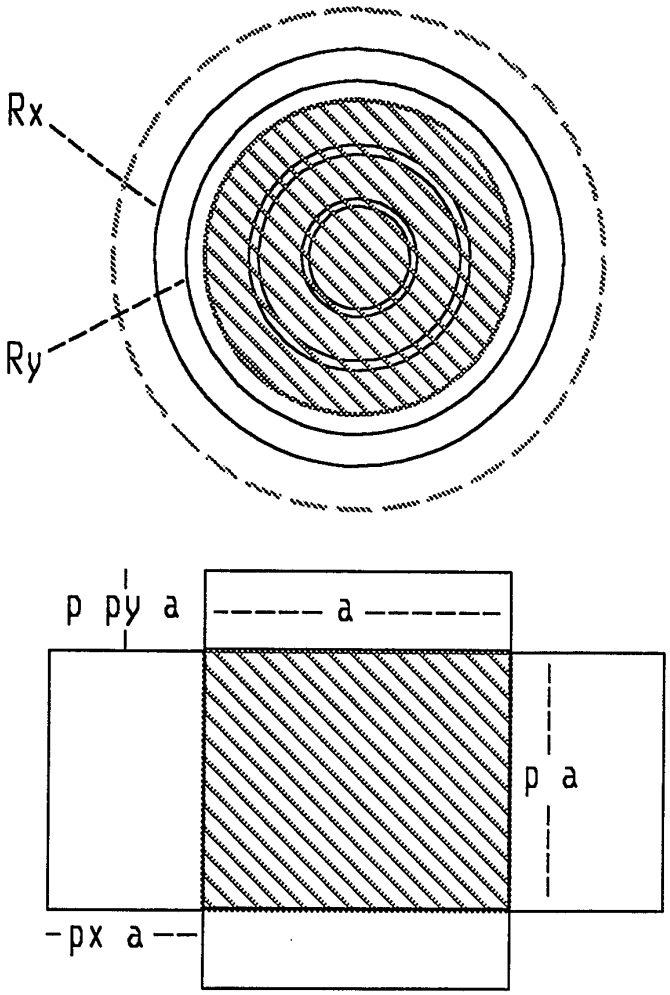
\includegraphics[width=.4\columnwidth]{mecs-geometry}
    \caption{Geometries of the absorber region and its vicinity in the supercell
      (top) and the diffusion solver mesh (bottom).
        The shaded and unshaded regions represent the homogenized absorber
        region and the adjacent non-absorber region, respectively.
        Retrieved from Fen et al.\ \cite{fen_modelling_1992}.}
    \label{fig:mecs-geometry}
\end{figure}

Figure \ref{fig:mecs-geometry} shows the 1-D cylindrical super cell for the
transport solver on the top and the corresponding 2-D Cartesian geometry for the
diffusion solver on the bottom. The four adjacent nodes in the Cartesian
geometry and their corresponding flux values are pairwise identical.\

According to the mesh-centered geometry in CITATION, the leakage $L$ is
calculated as:
%
\begin{gather}
  L = \frac{F_y\left(\phi_x-\phi_a\right)}{\frac{\delta_x}{D_a}+
    \frac{\Delta_x}{D_o}} + \frac{F_x\left(\phi_y-\phi_a\right)}{
  \frac{\delta_y}{D_a}+\frac{\Delta_y}{D_o}} \label{eq:mecs}
  \shortintertext{where}
  \begin{align}
    \phi_x =& \mbox{ flux in the $x$-neighbor nodes,} \nonumber \\
    \phi_y =& \mbox{ flux in the $y$-neighbor nodes,} \nonumber \\
    \phi_a =& \mbox{ flux in the absorber node,} \nonumber \\
    F_y =& \mbox{ surface area to $y$-neighbor nodes} = 2pa, \nonumber \\
    F_x =& \mbox{ surface area to $x$-neighbor nodes} = 2a, \nonumber \\
    \delta_x =& \mbox{ distance from the absorber node center to the
      $x$-surface} = a/2, \nonumber \\
    \delta_y =& \mbox{ distance from the absorber node center to the
      $y$-surface} = pa/2, \nonumber \\
    \Delta_x =& \mbox{ distance from the $x$-surface to the $x$-neighbor node
      center} = p_x a/2, \nonumber \\
    \Delta_y =& \mbox{ distance from the $y$-surface to the $y$-neighbor node
      center} = p p_y a/2, \nonumber \\
    a, p, p_x, p_y =& \mbox{ geometric parameters of the CITATION mesh geometry
      (Figure \ref{fig:mecs-geometry}),} \nonumber \\
    D_a =& \mbox{ diffusion coefficient in the absorber node,} \nonumber \\
    D_o =& \mbox{ diffusion coefficient in the neighboring nodes.} \nonumber
  \end{align}
\end{gather}

In the original formulation by Scherer \& Neef \cite{scherer_determination_1976}, they let
$D_a=D_o$. Taking leakage and flux values at $R_x$ and $R_y$ (figure \ref{fig:mecs-geometry}) from
the transport solver to be equal to the corresponding values in equation \ref{eq:mecs} yields a
value for $\phi_a$ representing the average flux in the absorber region. The equivalent
cross sections for each reaction type $i$ are then determined by matching reaction rates from the
transport calculation to the reaction rate as governed by diffusion theory as follows:
%
\begin{gather}
  \Sigma_i = \frac{A_i}{\phi_a V}
  \shortintertext{where}
  \begin{align}
    \Sigma_i =& \mbox{ macroscopic cross section of reaction type $i$,} \nonumber \\
    A_i =& \mbox{ reaction rate of reaction type $i$ from the transport calculation,} \nonumber \\
    V =& \mbox{ volume of the absorber region} = a^2 p. \nonumber
  \end{align}
\end{gather}

Fen et al.\ \cite{fen_modelling_1992} later provided an updated formulation by assuming that the
cross sections are accurate and instead determined the equivalent diffusion coefficient from Eq.
\ref{eq:mecs} and the transport leakage and flux values as follows:
%
\begin{gather}
  \frac{1}{D_a} = 2p\frac{\phi_x-\phi_a}{L}+\frac{2}{p}\frac{\phi_y-\phi_a}{L}
    -\frac{p_x+p_y}{2D_o}+\sqrt{R}
  \shortintertext{where}
  \begin{align}
    R =& \left(2p\frac{\phi_x-\phi_a}{L}+\frac{2}{p}\frac{\phi_y-\phi_a}{L}+
    \frac{p_x+p_y}{2D_o}\right)^2+4p\left(p_y-p_x\right)\frac{\phi_x-\phi_a}{L}
      \frac{1}{D_o} & \nonumber
  \end{align}
\end{gather}

As illustrated by the implementation in CITATION, \gls{MECS} requires considerable user input on
the supercell configuration to ensure that the leakage rates of the transport solution are
equivalent to the leakage rates of the subsequent diffusion solution. This procedure also places
some constraints on the location and size of the absorber node that can be inconsistent with the
nodalization of the rest of the reactor geometry \cite{ougouag_transport_2010}. \gls{MECS} is
incompatible with reactor geometries which contain control rods that are too close to each other
such that there is not enough distance in between to define neighboring nodes where
flux-equivalence is assumed. Lastly, \gls{MECS} is only applicable to coarse-mesh solvers and
homogenizes the control rod along with the adjacent material in its vicinity. Nevertheless,
\gls{MECS} has been widely used within the \gls{VSOP} suite of codes (which contains CITATION) for
\gls{HTGR} neutronic safety analyses
\cite{fen_modelling_1992, reitsma_evaluating_2003, mulder_neutronics_2020}.

\subsubsection{Response-Based Methods}

Like the \gls{MECS}, \textit{response-based methods} rely on response-function-based
transport methods to resolve the flux around absorber regions. In this context, coarse mesh/nodal
response functions relate quantities of interest of an individual node to input values from its
neighboring nodes. For instance, a response function may provide a node's average nodal flux and
outgoing partial currents in response to a given set of incident
partial fluxes from its neighboring nodes \cite{ougouag_transport_2010}. Transport solutions are
used to generate sets of response functions characterizing individual coarse meshes which contain
absorber regions. These response functions can be used directly or indirectly as modified boundary
conditions to accurately capture the effects of control rods on the global flux solution.

Fen et al.\ \cite{fen_modelling_1992} developed the \gls{RMM} which generates modified boundary
conditions from response functions to treat absorber nodes in whole-core diffusion calculations.
The response functions relate the incident partial current on one face of the node to the resultant
outgoing partial currents on all four faces of the same node. To be more precise, each incident
partial current of each neutron energy group on each face may contribute to the outgoing partial
current of any energy group on any face of the same node. The following equation for the response
matrix $A$ encapsulates the response values to be generated from the \gls{RMM}:
%
\begin{gather}
  A^{jk}_{nm} = \frac{J^{+j}_n}{J^{-k}_m} \mbox{ for } j,k=1...G \mbox{ and } n,m=1...N
  \label{eq:rmm} \\
  \shortintertext{where}
  \begin{align}
    A =& \mbox{ response matrix,} \nonumber \\
    N =& \mbox{ number of spatial intervals along the perimeter of the absorber node,} \nonumber \\
    J^{-k}_m =& \mbox{ incident partial current in energy group $k$ at spatial interval $m$,}
      \nonumber \\
    J^{+j}_n =& \mbox{ outgoing partial current in energy group $j$ at spatial interval $n$}
      \nonumber \\
    &\mbox{ in response to $J^{-k}_m$.} \nonumber
  \end{align}
\end{gather}

The \gls{RMM} compares favorably against the \gls{MECS} because it captures non-isotropic flux
effects from the non-central control rod location within the reactor core
\cite{fen_modelling_1992}. The \gls{RMM} also does not require the
meticulous tuning of adjacent node thicknesses to obtain equivalent fluxes to apply the \gls{MECS}.
However, both \gls{RMM} and \gls{MECS} involve precalculation procedures that must be rerun if the
absorber region is subjected to significant changes such as control rod withdrawal.

Rahnema et al.\ \cite{rahnema_advanced_2011} later developed an \gls{IDT} method that embeds the
transport correction for absorber regions in the full-core nodal diffusion calculation. Instead of
modified boundary conditions, the \gls{IDT} method generates coupling coefficients that are
morphologically identical to those used in nodal diffusion methods. The response region, which
contains the absorber region, is subdivided into several nodes. The transport correction
relies on higher-order spatial and angular response moments to maintain detailed responses between
adjacent response nodes. Changes in the response region can be modeled by swapping out response
nodes without having to rerun the transport solver to generate new coupling coefficients. The
intra-response region calculations were iteratively coupled to the full-core diffusion calculations
to avoid introducing additional off-diagonal terms, which would increase the solve time of an
otherwise tri-diagonal system of nodal diffusion equations. In several verification studies of
static \gls{HTGR} core configurations, the \gls{IDT} method produced similar eigenvalue and flux
distribution results \cite{rahnema_advanced_2011} as the \gls{RMM}. However, they did not
demonstrate the response region swapping that the \gls{IDT} was designed for.

\subsubsection{Ronen Method}

Ronen \cite{ronen_accurate_2004} postulated an alternative formulation for diffusion coefficients
based on neutron currents from transport calculations.
Fick's law of diffusion is valid under three assumptions: the neutron flux gradient is small, the
absorption-to-scattering ratio is small, and scattering sources are isotropic. Therefore, diffusion
theory fails for anisotropic fluxes in and near absorber regions. The Ronen method proposes using
the integral form of the transport equation to derive transport operators for the neutron current
and substituting the values into Fick's first law of diffusion (Eq. \ref{eq:fick}) to obtain
space-dependent diffusion coefficients as follows:
%
\begin{align}
  D(\vec{r},E) =& -\frac{J_{tr}(\vec{r},E)}{\nabla \phi(\vec{r},E)}
  \label{eq:ronen}
  \shortintertext{where}
    J_{tr} =& \mbox{ transport-derived neutron current.} \nonumber
\end{align}

In doing so, the Ronen method provides pointwise corrections to the diffusion equation, overcoming
the small flux gradient limitation. Tomatis \& Dall'Osso \cite{tomatis_application_2011}
numerically implemented the Ronen method for a 1-D homogeneous slab with two energy groups and
isotropic scattering. Instead of using Eq. \ref{eq:ronen}, which showed instabilities near flat
flux regions where the denominator approaches zero, they calculated corrections to the diffusion
coefficients at cell interfaces using the difference between the transport- and diffusion-derived
currents as follows:
%
\begin{align}
  \delta D(x_{i+1/2},E) =& -\delta J(x_{i+1/2},E) \frac{(\Delta x_{i+1}+\Delta x_i)/2}{
  \phi(x_{i+1},E)+\phi(x_i,E)} \label{eq:tomatis}
  \shortintertext{where}
    x_i =& \mbox{ $i$-th spatial interval,} \nonumber \\
    \delta J(x,E) =& J_{tr}(x,E) - J_D(x,E), \nonumber \\
    \Delta x_i =& \mbox{ size of $i$-th spatial interval.} \nonumber
\end{align}

They derived expressions for the transport operators for $J_{tr}$ in terms of exponential integral
functions and Legendre expansions of the angular flux.
Gross et al.\ \cite{gross_high-accuracy_2020} extended the derivation of the transport operators to
handle 1-D heterogeneous problems in the form of fuel assemblies with fuel, water, and fuel+absorber
regions. Tomatis et al.\ \cite{tomatis_ronen_2021} developed new numerical implementations for 1-D
slab, cylindrical, and spherical geometries by employing probabilistic treatments from the
\gls{CPM} \cite{lewis_computational_1984} for the transport operators. The authors also implemented
a solver acceleration scheme which helped with the poor convergence rate observed in the earlier
studies \cite{tomatis_application_2011, gross_high-accuracy_2020}.

All three studies showed improvements in flux solutions with the Ronen method over
pure diffusion solvers in all of the test cases, particularly for a 1-D heterogeneous
\gls{BWR}-based problem with isotropic scattering and strong absorption cross sections
\cite{gross_high-accuracy_2020}. The error in reactivity values for three different \gls{BWR}
configurations differed from the reference $S_{16}$ transport calculations by at most 62 pcm after
one hundred iterations ($1$ pcm $=10^{-5}$) . However, the demonstrations were limited to simple
1-D geometries. Although the authors provided derivations for anisotropic scattering, their test
cases incorporated only isotropic scattering. The derivation of semi-analytic transport operators
from the integral form of neutron transport equations would be much more complicated
for more complex reactor geometries in 2-D or 3-D similar to how analytical solution forms do not
exist beyond those for simple geometries.

\subsubsection{Averaged Eddington Factors and High-Order Empirical Diffusion Coefficients}

Similarly, Pounders \& Rahnema developed two different methods for generating space-dependent
diffusion coefficients \cite{pounders_diffusion_2009}. Both methods possess the same caveat in
requiring \textit{a priori} knowledge of the flux and current. The first method, called the
\gls{AEF} method, relies on the Eddington factor, which is defined as the second angular moment of
the angular flux normalized by its zeroth moment. In 1-D, the Eddington factor is given as:
%
\begin{align}
  E_g(z) =& \frac{\int^1_{-1} \mu^2\psi(z,\mu)d\mu}{\int^1_{-1} \psi(z,\mu)d\mu}
\end{align}
%
The $g$ subscript denotes the discrete neutron group index of the multigroup diffusion equations
obtained from discretizing the continuous energy variable, as described in Section
\ref{sec:summary-nts-mtds}. The Eddington factor features in the first angular moment of the
1-D multigroup transport equations, obtained by multiplying the transport equation throughout by
the cosine of the scattering angle $\mu=\cos\theta$ and integrating over $\mu=-1$ to $\mu=1$:
%
\begin{gather}
  \frac{d\left[E_g(z)\phi_g(z)\right]}{dz} + \Sigma_{t,g}(z)J_g(z) = \sum^G_{g'=1}
  \Sigma^{g'\rightarrow g}_{s1}(z)J_{g'}(z) \label{eq:bte-1st-mom}
  \shortintertext{where}
    \Sigma^{g'\rightarrow g}_{s1} = \int^1_{-1} \mu \Sigma_s d\mu \nonumber
\end{gather}
%
Assuming the Eddington factor varies slowly in space, we can approximate Eq. \ref{eq:bte-1st-mom}
as:
%
\begin{gather}
  E_g(z)\frac{d\bar{\phi}_g(z)}{dz} + \Sigma_{t,g}(z)\bar{J}_g(z) = \sum^G_{g'=1}
  \Sigma^{g'\rightarrow g}_{s1}(z)\bar{J}_{g'}(z) \mbox{ for } z \in V_i \label{eq:bte-1st-est}
  \shortintertext{where}
  \begin{align}
    \bar{\phi}_g =& \mbox{ approximate flux solution of Eq. \ref{eq:bte-1st-est},} & \nonumber \\
    \bar{J}_g =& \mbox{ approximate current solution of Eq. \ref{eq:bte-1st-est},} & \nonumber \\
    V_i =& \mbox{ a subvolume of the system domain.} & \nonumber
  \end{align}
\end{gather}
The overbars distinguish the approximate solutions of Eq. \ref{eq:bte-1st-est} from the true
solution of Eq. \ref{eq:bte-1st-mom}. From Eq. \ref{eq:bte-1st-est}, the diffusion coefficient can
be defined as:
%
\begin{align}
  D_g(z) = E_g(z)\left[\Sigma_{t,g}(z)-\sum^g_{g'=1}\Sigma^{g'\rightarrow g}_{s1}(z)
  \frac{\bar{J}_{g'}(z)}{\bar{J}_g(z)}\right]^{-1} \label{eq:diffcoef-edd}
\end{align}
By further assuming that the Eddington factors are piecewise constant in each subvolume $V_i$, the
averaged Eddington factor $E^i_g$ can be evaluated as:
%
\begin{align}
  E^i_g =& \frac{E_g(z_{i+1})\phi_g(z_{i+1})-E_g(z_i)\phi_g(z_i)}{\bar{\phi}_g(z_{i+1})-
  \bar{\phi}_g(z_i)}
  \shortintertext{where}
  z_{i+1} =& \mbox{ upper bound of subvolume $V_i$,} \nonumber \\
  z_i =& \mbox{ lower bound of subvolume $V_i$.} \nonumber
\end{align}
%
The diffusion coefficient from Eq. \ref{eq:diffcoef-edd} can then be calculated as:
%
\begin{align}
  D^{AEF}_g(z) =& E^i_g\left[\hat{\Sigma}_{t,g}-\sum^G_{g'=1}\hat{\Sigma}^{g'\rightarrow g}_{s1}
  \frac{\hat{J}_{g'}}{\hat{J}_g}\right]^{-1}
  \shortintertext{where}
  \hat{\Sigma}_{t,g} =& \frac{\int_{V_i}\Sigma_{t,g}(z)J_g(z)dz}{\int_{V_i}\bar{J}_g(z)dz},
  \nonumber \\
  \hat{\Sigma}^{g'\rightarrow g}_{s1} =& \frac{\int_{V_i}\Sigma^{g'\rightarrow g}_{s1}(z)J_{g'}(z)
  dz}{\int_{V_i}\bar{J}_{g'}(z)dz}, \nonumber \\
  \hat{J}_g =& \int_{V_i} \bar{J}_g(z)dz. \nonumber
\end{align}

The second method employs a much more straightforward premise: Fick's law is assumed to be
accurate, with
high-order empirical diffusion coefficients to be determined. Given a known transport
solution, the following integration holds for a small homogeneous volume $V_i$:
%
\begin{align}
  \frac{1}{V_i}\int_{V_i}J_g(z)dV =& -\frac{1}{V_i}\int_{V_i}D_g(z)\frac{d\phi_g(z)}{dz}dV.
\end{align}
%
Taking $D_g$ to be constant in $V_i$, we may apply the divergence theorem to obtain
%
\begin{align}
  \bar{J}_gV_i =& -D^i_g\int_{\partial V_i} \phi_g(z)dA
  \shortintertext{where}
  \bar{J}_g =& \mbox{ average current in $V_i$,} \nonumber \\
  \partial V_i =& \mbox{ bounding surface of $V_i$.} \nonumber
\end{align}
%
Rearranging the terms, we may obtain the empirical diffusion coefficient formulation from the
transport-derived flux and current as follows:
%
\begin{align}
  D^i_g =& -\frac{\left(z_{i+1}-z_i\right) \bar{J}_g}{\left[\phi_g(z_{i+1})-\phi_g(z_i)\right]}
  \label{eq:emp}
\end{align}
%
Both \gls{AEF} and empirical methods require the respective subvolumes $V_i$ to be small enough
for the assumptions of constant Eddington factors and diffusion coefficients to hold within $V_i$.

Both methods performed much better than conventional diffusion coefficients derived using the
$P_1$ approximation method. For the same 1-D heterogeneous \gls{BWR} problem demonstrating the prior
Ronen method \cite{gross_high-accuracy_2020} but with anisotropic scattering, the absolute errors
in $k_{eff}$ are around 100 pcm after eliminating errors associated with energy group
condensation. The error values compare favorably with the 159-683 pcm error with the $P_1$ method.
The \gls{AEF} and empirical methods also reproduced the flux distributions better with a maximum
pointwise error of 2\% as opposed to 5\% from the $P_1$ method. Similar to the Ronen method, the
\gls{AEF} and empirical methods introduce pointwise corrections with information from transport
methods. However, both \gls{AEF} and empirical methods require a priori knowledge of the true
solution or otherwise
accurate estimates from transport methods. In contrast, the Ronen method relies on analytical
transport operators, which use diffusion flux estimates from the previous iteration to update the
flux solution. Nevertheless, the \gls{AEF} and empirical methods provide the foundation for further
development of practical, self-closing transport-correction techniques.

\subsubsection{General Equivalence Theory and Superhomogenization Method}

As mentioned in Section \ref{sec:summary-nts-mtds}, coarse-mesh and nodal methods homogenize
heterogeneities in reactor geometries to reduce the computational costs of running full-core
simulations. Equivalence techniques which reduce spatial homogenization error are also effective
for accurately modeling the integral worths of control rods within fuel assemblies. The \gls{GET}
\cite{koebke_new_1980, smith_nodal_1983} and \gls{SPH} \cite{kavenoky_sph_1978,
hebert_consistent_1991} methods represent the most widely used equivalence methods for improving
the performance of diffusion calculations in homogenized \gls{LWR} models. Both methods involve
deriving additional homogenization parameters from single-assembly transport calculations with
reflective boundary conditions. Since the transport calculation step is already a prerequisite
for generating homogenized group constants, the equivalence methods are simple to implement and
impose reasonably small additional computational costs.

Koebke \cite{koebke_new_1980} first proposed abandoning continuous surface fluxes to preserve net
surface currents through discontinuity factors. Smith \cite{smith_assembly_1986}
later extended this concept to assembly-homogenized calculations. The discontinuity factors are
calculated for each face of the homogenized region to preserve volumetric reaction rates and
surface neutron currents. The discontinuity factors are calculated as follows:
%
\begin{gather}
  DF = \frac{\phi^{het,sur}}{\phi^{hom,sur}}
  \shortintertext{where}
  \begin{align}
    DF =& \mbox{ discontinuity factor,} \nonumber \\
    \phi^{het,sur} =& \mbox{ surface flux of the region from the heterogeneous calculation,}
    \nonumber \\
    \phi^{hom,sur} =& \mbox{ surface flux of the region from the homogeneous calculation.}
    \nonumber
  \end{align}
\end{gather}
%
\gls{GET} was later extended for fine mesh calculations \cite{yamamoto_cell_2004}, which refers to
cell-level homogenization; each fuel cell in an assembly, consisting of the fuel pellet, cladding,
and moderator, is individually homogenized as opposed to lumping together the entire assembly.

In contrast, the \gls{SPH} method, first proposed by Kavenoky \cite{kavenoky_sph_1978} for
irregular lattices and later applied as a cell-homogenization technique by Hebert
\cite{hebert_consistent_1991}, introduces correction factors to homogeneous cross sections as
follows:
%
\begin{gather}
  \tilde{\Sigma}^{hom}_k = \mu_k \Sigma^{hom}_k
  \shortintertext{where}
  \begin{align}
    \tilde{\Sigma}^{hom}_k =& \mbox{ \gls{SPH}-corrected homogeneous cross section for region $k$,}
    \nonumber \\
    \mu_k =& \mbox{ \gls{SPH} correction factor for region $k$,} \nonumber \\
    \Sigma^{hom}_k =& \mbox{ uncorrected homogeneous cross section for region $k$.} \nonumber
  \end{align}
\end{gather}
%
The \gls{SPH} factor is calculated as follows:
%
\begin{gather}
  \mu_k = \frac{\bar{\phi}^{het}_k}{\phi^{hom}_k}
  \shortintertext{where}
  \begin{align}
    \bar{\phi}^{het}_k =& \mbox{ average flux in region $k$ from the heterogeneous calculation,}
    \nonumber \\
    \phi^{hom}_k =& \mbox{ average flux in region $k$ from the homogeneous calculation}
    \nonumber \\
                  & \mbox{ with \gls{SPH}-corrected cross sections.} \nonumber
  \end{align}
\end{gather}

The \gls{GET} and the \gls{SPH} methods are designed to preserve reaction rates at the assembly
level \cite{yamamoto_cell_2004}. Given that the \gls{SPH} method introduces only one correction
factor per cell, it only preserves the average net current across all surfaces as opposed
to the net current at each surface with \gls{GET}. Similarly, the isotropic nature of \gls{SPH}
factors leads to worse pin-power estimates near control rods and reflectors compared to \gls{GET}.
However, the \gls{SPH} method is simpler to implement in the diffusion solver as the \gls{SPH}
factors can be precombined with the cross sections to generate \gls{SPH}-corrected cross sections.
\gls{GET} requires diffusion solvers, which allow for flux discontinuities at the interfaces.
Furthermore, \gls{GET} requires more memory to store up to six discontinuity factors, one for each
mesh surface, in 3-D calculations.

Modeling control rods in full-core calculations with the \gls{SPH} method or \gls{GET} provides
better estimates of the multiplication factor and the flux distribution than reference diffusion
solutions. In this regard, the correction factors do not distinguish between errors arising from
homogenization or the diffusion approximation. However, the improved solutions, especially with the
\gls{SPH} method, can still deviate significantly from reference transport calculations. A
supercell, similar to the one adopted by \gls{MECS}, can be used to reduce errors within and near
control rod cells \cite{ortensi_newton_2018}. Another disadvantage, shared by other schemes
dependent on homogenization, is that homogenization removes some of the heterogeneity in the flux
and temperature.

\subsubsection{Multilevel Quasi-Diffusion Method}

In 1964, Gol'din \cite{goldin_quasi-diffusion_1964} originally developed the \gls{QD} method
as an acceleration scheme for the solution of the neutron transport equation. Consider the
steady-state, single-group neutron transport equation:
%
\begin{gather}
  \hat{\Omega}\cdot\nabla\psi(\vec{r},\hat{\Omega}) + \Sigma_t(\vec{r})\psi(\vec{r},\hat{\Omega}) =
  \int_{4\pi}d\hat{\Omega}'\ \Sigma_s(\vec{r},\hat{\Omega}'\rightarrow\hat{\Omega})
  \psi(\hat{\Omega}') + Q(\vec{r},\hat{\Omega}) \label{eq:qd-high}
  \shortintertext{where}
  Q = \mbox{ external source term.} \nonumber
\end{gather}
%
Take the zeroth and first angular moments to obtain the following two equations, respectively:
%
\begin{gather}
  \nabla\cdot J(\vec{r}) + \Sigma_t(\vec{r})\phi(\vec{r}) = \Sigma_{s,0}(\vec{r})\phi(\vec{r}) +
  Q_0(\vec{r}) \label{eq:qd-low-0th} \\
  \nabla\cdot\left(\vec{\vec{E}}(\vec{r})\phi(\vec{r})\right) + \Sigma_t(\vec{r})J(\vec{r}) =
  \Sigma_{s,1}(\vec{r})J(\vec{r}) + Q_1(\vec{r}) \label{eq:qd-low-1st}
  \shortintertext{where}
  \begin{align*}
    \phi(\vec{r}) =& \int_{4\pi}d\hat{\Omega}\ \psi(\vec{r}), & \\
    J(\vec{r}) =& \int_{4\pi}d\hat{\Omega}\ \hat{\Omega}\psi(\vec{r}), & \\
    Q_0(\vec{r}) =& \int_{4\pi}d\hat{\Omega}\ Q(\vec{r},\hat{\Omega}), & \\
    Q_1(\vec{r}) =& \int_{4\pi}d\hat{\Omega}\ \hat{\Omega}Q(\vec{r},\hat{\Omega}), & \\
    \Sigma_{s,l} =& \mbox{ $l$th Legendre moment of the scattering cross section $\Sigma_s$,} & \\
    \vec{\vec{E}} =& \frac{\int_{4\pi}d\hat{\Omega}\ \hat{\Omega}\hat{\Omega}\psi(\vec{r})}{
    \int_{4\pi}d\hat{\Omega}\ \psi(\vec{r})}. &
  \end{align*}
\end{gather}
%
The Eddington tensor $\vec{\vec{E}}$ captures flux anisotropies from the high-order transport
solution of Eq. \ref{eq:qd-high} and enables the low-order Eqs. \ref{eq:qd-low-0th} \&
\ref{eq:qd-low-1st} to accurately reproduce the high-order flux solution. These equations form a
two-level acceleration scheme. The solution algorithm is as follows:
%
\begin{enumerate}
  \item Initialize $\phi^l$ with an initial scalar flux distribution $\phi^0$
  \item Solve Eq. \ref{eq:qd-high} for $\psi^{l+1/2}$ using $\phi^l$
  \item Generate Eddington factors $\vec{\vec{E}}$ using $\psi^{l+1/2}$
  \item Solve Eqs. \ref{eq:qd-low-0th} \& \ref{eq:qd-low-1st} for $\phi^{l+1}$
  \item Repeat Steps 2-4 until flux convergence is reached
\end{enumerate}

The high- and low-order formulations produce the same scalar flux solution only if they share the
same spatial discretization scheme. Otherwise, the fluxes will differ by a spatial truncation
error \cite{adams_fast_2002}. The Eddington tensor converges significantly faster than the angular
fluxes, thus accelerating the neutron transport method by effectively replacing some of the
high-order iterations with the low-order iterations. Gol'din \cite{anistratov_solution_1986} later
extended the \gls{QD} method for multigroup neutron transport problems with anisotropic scattering.
\gls{QD} methods for multigroup neutron transport problems typically adopt three levels instead of
the two levels described by Eqs. \ref{eq:qd-high}, \ref{eq:qd-low-0th}, and \ref{eq:qd-low-1st}.
The three levels consist of the multigroup high-order neutron transport equations, the multigroup
low-order \gls{QD} equations, and the effective gray (one-group) low-order \gls{QD} equations
\cite{anistratov_solution_1986}. The gray low-order equations are derived through flux-averaging of
the multigroup neutron group constants and a closure relation across all energy groups.

Tamang \& Anistratov \cite{tamang_multilevel_2014} applied the multilevel \gls{QD} method to
time-dependent multiphysics neutron transport and heat transfer problems by iteratively coupling
the gray low-order equations to the heat transfer equations. Their coupling algorithm takes
advantage of the lower computational cost of the low-order equations to quickly resolve
multiphysics interactions during inner iterations, thereby requiring fewer outer iterations and
high-order transport calculations. Reynolds \& Palmer \cite{reynolds_analysis_2023} implemented the
multilevel \gls{QD} method in RZ cylindrical coordinates and the capability to model \gls{DNP} flow
for simulating molten salt reactor kinetics.

The multilevel \gls{QD} method may accurately model control rod provided that the method utilizes
sufficient fidelity in the high-order transport calculations. In particular, Reynolds \& Palmer
demonstrated this through a steady-state simulation of a 2-D axisymmetric, two-group \gls{MSRE}
model with a partially-inserted control rod. Their \gls{QD} method implementation with the $S_{12}$
method for the high-order transport iterations allowed for more accurate neutron flux estimates
near the control rod compared to a $P_1$ method. However, multilevel \gls{QD} methods still have
computational costs comparable to accelerated neutron transport methods, which remain too
computationally intensive for time-dependent 3-D full-core calculations.

\subsubsection{Hybrid Methods via Spatial Domain Decomposition}

Given the high computational costs of neutron transport calculations, hybrid methods have been
developed by decomposing the problem domain into \textit{transport} and \textit{diffusive}
subdomains. The neutron flux in diffusive subdomains may be resolved sufficiently accurately using
low-order methods such as neutron diffusion, $P_1$, or $S_2$ to provide significant computational
cost savings.

One type of approach for hybrid methods involves making predetermined domain decompositions prior
to the neutron flux calculation. These methods would require interface conditions at the
transport-diffusion interfaces to couple adjoining subdomains. Griffin
\cite{prince_neutron_2024}, a \gls{MOOSE}-based reactor multiphysics software, employs this
approach for its $S_N$-$P_N$ \textit{multischeme} transport method. Griffin provides two options
for the interface
conditions: the Lagrange multiplier and the upwinding methods \cite{wang_hybrid_2017}. The Lagrange
multiplier method enforces the continuity of angular flux moments at the interface through Lagrange
multipliers minimizing the differences in the moments at the interface. The angular flux moments on
$S_N$ side typically require smoothing due to the $S_N$ method's discrete treatment of the angular
dependence. The upwinding method is a more conventional scheme that maintains
causality by generating surface source boundaries on
either side of the interface based on the outgoing neutron currents from the opposing neutron
transport scheme. The upwinding method does not require smoothing on the $S_N$ side of the
interface and is applicable to discontinuous numerical solvers, but the flux solutions are
generally discontinuous across the interface. The weak formulation of the Lagrange multiplier
interface condition is:
%
\begin{gather}
  -\int_S \left[\left(\llbracket\Psi\rrbracket,\Lambda^*\right)_{\Gamma} +
  \left(\llbracket\Psi^*\rrbracket,\Lambda\right)_{\Gamma}\right] d\hat{\Omega}
  \shortintertext{where}
  \begin{align}
    \llbracket\Psi\rrbracket &= \Psi^+ - \Psi^-, \nonumber \\
    \Psi^\pm &= \lim_{s\rightarrow 0^+} \Psi(\vec{x}+s\hat{n}), \nonumber \\
    \Lambda &= \mbox{ Lagrange multiplier}, \nonumber \\
    \Gamma &= \mbox{ interface boundary}, \nonumber \\
    \hat{n} &= \mbox{ normal vector at interface boundary}, \nonumber
  \end{align}
\end{gather}
%
and the weak formulation of the upwinding method is:
%
\begin{gather}
  \int_S \left(|\hat{\Omega}\cdot\hat{n}|\llbracket\Psi^*\rrbracket,\Psi^-\right)_{\Gamma^+}
  d\hat{\Omega} -
  \int_S\left(|\hat{\Omega}\cdot\hat{n}|\llbracket\Psi^*\rrbracket,\Psi^+\right)_{\Gamma^-}
  d\hat{\Omega}
\end{gather}
%
The terms with asterisks denote test functions used in the \gls{FEM} framework.

Two recent works by Anistratov \& Stehle \cite{anistratov_computational_2012} and Stehle et al.\
\cite{stehle_hybrid_2014} describe another approach that is distinct from the prior approach in
two ways. Firstly, they developed an on-the-fly scheme for estimating a transport metric which can
indicate whether a subregion is diffusive. The solver uses this information to apply adaptive
domain decomposition and decide which subregions require transport calculations for solution
accuracy. Secondly, they employ a two-level neutronics method similar to the multilevel \gls{QD}
method to obtain the neutron flux solution. The hybrid method evaluates the low-order neutron
diffusion problem on the entire problem domain while limiting high-order transport calculations to
\textit{transport} subregions. The low-order formulation also serves as an acceleration scheme to
the high-order formulation to provide greater computational cost savings. The authors showed the
viability of using Eddington tensor estimates as the metric for quantifying transport effects in
a subregion. The Eddington tensor is identical to one defined for the \gls{QD} scheme. The
two-level neutronics method is based on the \textit{Second-Moment} method developed by Lewis \&
Miller \cite{lewis_comparison_1976}. The low-order second-moment equations are:
%
\begin{gather}
  \nabla\cdot J^{(s+1)}+\Sigma_a\phi^{(s+1)} = q, \label{eq:2nd-moment-1} \\
  \frac{1}{3}\nabla\cdot\phi^{(s+1)}+\Sigma_t J^{(s+1)} = \nabla\cdot F^{(s+1/2)}
  \label{eq:2nd-moment-2}
  \shortintertext{where}
  F^{(s+1/2)}_{\alpha\beta} = \int_{4\pi}
  \left(\frac{1}{3}\delta_{\alpha\beta}-\Omega_\alpha\Omega_\beta\right)
  \Psi^{(s+1/2)} d\Omega \label{eq:2nd-moment-3}
\end{gather}
%
$(s)$ denotes the iteration index. $F$ is a transport correction tensor calculated from the
high-order neutron transport equations in \textit{transport} subregions. $F$ is simply set to zero
in \textit{diffusive} subregions. The scalar flux from the low-order equations is also used to
evaluate the 0th-order scattering source term and accelerate the high-order calculations for
$\Psi^{(s+1/2)}$. Stehle et al.\ \cite{stehle_hybrid_2014} demonstrated their hybrid method on two
2-D, single-group test problems. Both problems consisted of two regions with idealized macroscopic
cross sections representing \textit{transport} and \textit{diffusive} regions with high absorption
and scattering ratios, respectively.

\section{Summary}

In the last two decades, many \gls{MSR} multiphysics software have been developed by
extending existing reactor software such as DALTON and \gls{TRACE} for \gls{MSR} modeling or
building on general multiphysics software frameworks such as OpenFOAM and \gls{MOOSE}. The
resultant software have a wide range of capabilities arising from their calculation schemes,
constraints from legacy code, and simplifying assumptions to balance computational costs. Several
research efforts have been targeted at establishing benchmarks for \gls{MSR} simulation tool
\gls{VV}, notably with the CNRS benchmark \cite{tiberga_results_2020} and neutronics benchmarks of
the \gls{MSRE} \cite{fratoni_molten_2020} and the \gls{MSFR} \cite{brovchenko_neutronic_2019}.
While these efforts have plugged significant technical gaps, more can be done to develop open
\gls{VV} benchmarks for multiphysics \gls{MSR} modeling, particularly for model verification of
\gls{DNP} drift out of the active core region. Among other considerations, the proposed
verification model should provide the necessary group constant input data for other multiphysics
simulation tools to replicate the results without discrepancies propagating from using different
nuclear databases or stochastic uncertainties from Monte Carlo simulations.

On the \gls{TH}-modeling side of \gls{MSR} multiphysics, turbulent flow is a complex, yet important
phenomenon to include in our simulation models to obtain accurate predictions of \gls{MSR} behavior
under various operating conditions. Most \gls{MSR} multiphysics studies with turbulence models rely
on the two-equation turbulence models, which provide acceptable estimates of time-averaged flow
characteristics. One study \cite{podila_cfd_2019} showed close agreement in the \gls{MSRE}
temperature distribution with various one-equation, two-equation, and \gls{RSM} turbulence
models despite relatively larger differences observed in turbulence intensities near the walls.
This observation suggests one-equation models may be adequate for \gls{MSR} designs and simulations
with weaker turbulent effects, although other analyses may require even more accurate turbulence
models like \gls{DES} to capture turbulent effects without time averaging adequately.

Lastly, there is a lack of research focus into robust techniques for accurate control rod modeling
for time-dependent \gls{MSR} analyses. Control rods induce highly anisotropic fluxes within
themselves and their vicinities.
Unfortunately, higher-fidelity neutron transport methods are typically too computationally
expensive for multiphysics \gls{MSR} simulations, while faster methods like neutron
diffusion perform poorly in regions with highly anisotropic fluxes. However, transport-correction
techniques can be applied to augment neutron diffusion calculations in these regions. While few
have been applied to \gls{MSR} multiphysics simulations other than albedo boundary conditions,
various techniques have been proposed and implemented for other reactor types. Helpful information
may be gleaned from these techniques to improve control rod modeling in \glspl{MSR} with the
neutron diffusion method.

\glsresetall

\chapter{Verification of Multiphysics Features in Moltres}
\label{chap:verification}
%\section{Description of Moltres} \label{sec:moltres-description}

This chapter provides an overview of Moltres as a multiphysics
simulation software for molten salt reactors. 
Section \ref{sec:moltres-features}
describes the general software features of Moltres, Section
\ref{sec:moltres-physics} expands on the physics models in Moltres, and Section
\ref{sec:moltres-previous} describes previous work on \gls{MSR} analysis with Moltres to illustrate
its current capabilities and limitations.

\subsection{General Features} \label{sec:moltres-features}

This section discusses the general software features of Moltres. The
discussion focuses on robustness, extensibility, and ease of use
since these characteristics represent the hallmarks of good multiphysics
software \cite{keyes_multiphysics_2013}. These criteria also apply to
assessing \gls{MSR} simulation tools since the nonlinearity of \gls{MSR}
multiphysics analysis and the complexity of advanced reactor designs
necessitate robust, scalable, and flexible computational tools.

Moltres draws many advantages from being developed on MOOSE
\cite{giudicelli_30_2024}. MOOSE is an open-source, finite-element,
multiphysics framework developed at \gls{INL}. The framework provides a
user-friendly interface for developing multiphysics software through
\gls{OOP} in \texttt{C++} to modularize various
functions relevant to finite-element multiphysics solvers. In this approach,
MOOSE and MOOSE-based applications break down \glspl{PDE} into individual terms
and store them as individual \texttt{C++ objects} referred to as
\texttt{Kernels}. These \texttt{Kernels} contain functions for calculating
their weak form residual and Jacobian
contributions and other relevant functions required to solve a given
\gls{PDE}. \gls{OOP} in MOOSE simplifies software development
since developers can write new \texttt{Kernels} as child classes in
\texttt{C++} derived from existing \texttt{Kernels} (base classes), which share
similar physics to inherit common functions.
The same philosophy applies to all other systems in MOOSE, such as
the \texttt{BCs}, \texttt{Materials}, and \texttt{Postprocessor}
systems for handling relevant boundary conditions, material properties, and
postprocessing calculations, respectively. Overall, this approach also saves
researchers time and effort since they are unencumbered by the technical details
and complexities of programming efficient computational tools for
numerical analysis.

\begin{figure}[htb!]
	\centering
	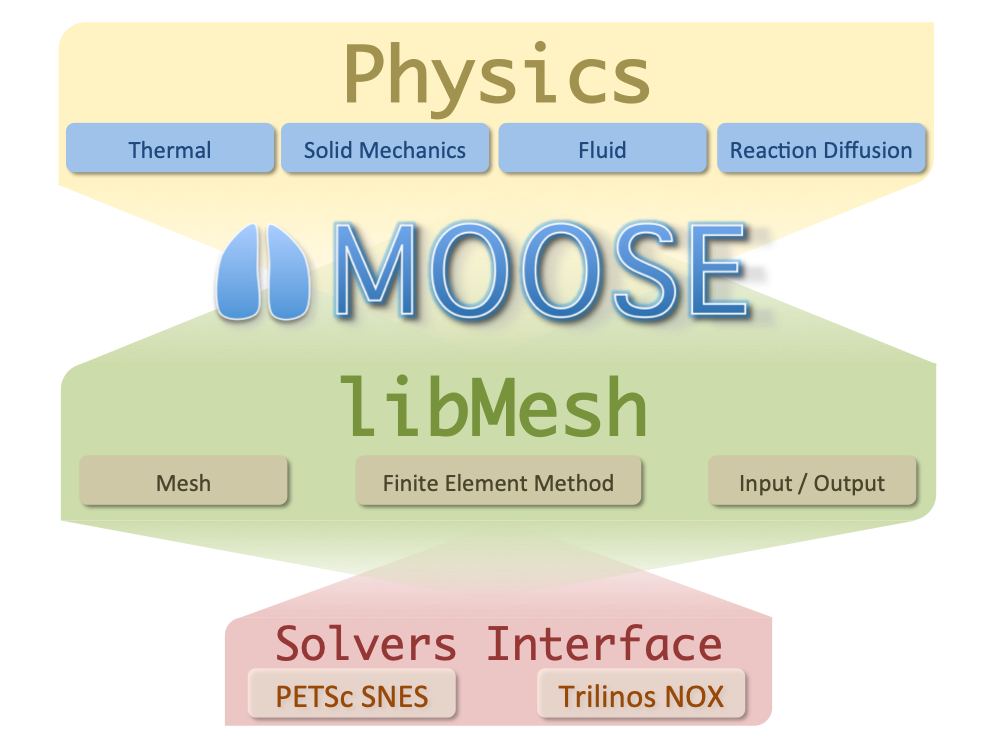
\includegraphics[width=.7\columnwidth]{moose}
	\caption{Structure of MOOSE and its dependencies.}
	\label{fig:moose}
\end{figure}

MOOSE relies on two other open-source libraries: libMesh
\cite{kirk_libmesh_2006} for its \gls{FEM} capabilities on unstructured mesh
and PETSc \cite{satish_petsc_2019} for its nonlinear solvers and
preconditioning routines. By extension, Moltres gains access to these
sophisticated numerical analysis tools and benefits from their continuous
development. Figure
\ref{fig:moose} shows how MOOSE serves as an interface between physics
applications and libMesh/PETSc. MOOSE supports
modeling on up to three-dimensional (3-D) unstructured meshes for a wide range
of mesh file formats, including the commonly used Exodus II file format. For
2-D meshes, users can opt between Cartesian and polar RZ coordinates. MOOSE
also supports parallel computing through the \gls{MPI} library to leverage
modern high-performance computing for large multiphysics simulations.

Moltres benefits from the highly-integrated cross compatibility within the
ecosystem of MOOSE-based applications. MOOSE facilitates multiphysics coupling
among all MOOSE-based applications by providing a common framework for shared
data access and file input/output, thus eliminating computational costs from
data transfers and allowing for fully coupled simulations. For example, Moltres
can couple with the \texttt{Navier-Stokes} module \cite{peterson_overview_2018}
from MOOSE for fully coupled reactor simulations modeling neutronics and
thermal-hydraulics with incompressible flow modeling. Section
\ref{sec:msr-multiphysics} highlighted the advantages of fully coupled schemes
for modeling strongly coupled systems, such as the coupled
neutronics and thermal-hydraulics in \glspl{MSR}. Moltres can also easily
couple to other MOOSE-based applications in a similar fashion. In
addition, MOOSE
provides the option for either tight or loose coupling through the
\texttt{MultiApp} system \cite{gaston_physics-based_2015}. Tight coupling
schemes can outperform fully coupled schemes in weakly coupled systems in which
the computational expenses of fully coupled schemes outweigh the savings from
running fewer Newton iterations due to the superior convergence rate. Loose
coupling schemes help accelerate time-dependent simulations of
stable systems towards a steady state if only the steady-state
configuration interests the user. This situation may occur in the later
stages of \gls{MSR} simulations when the \gls{DNP}
concentrations converge slowly due to their relatively large decay half-lives.
Furthermore, segregated solvers through the \texttt{MultiApp} system enable
Moltres to introduce \gls{DNP} drift and non-uniform
temperature distributions into criticality search simulations. Regardless of
which coupling scheme works best, MOOSE-based applications provide the flexibility
to switch among the schemes as users see fit. For time-dependent simulations,
MOOSE provides more than ten implicit and explicit timestepping
schemes. The default scheme is the first-order backward Euler
method which offers excellent solver stability for stiff \glspl{PDE}.

Lastly, Moltres is an open-source \gls{LGPL} software hosted on
GitHub \cite{github_build_2017}. Open-sourcing software provides ease of access
and expands the user base. These characteristics promote software quality
through increased feedback on users' needs and transparency for peer review.
Open-source software accelerate research progress by supporting
collaboration and sharing best software practices. Supporting Moltres'
continued development, Moltres relies on GitHub for online version control with
continuous integration testing to protect its existing capabilities.

In summary, Moltres provides robust and flexible coupling capabilities to
model strongly coupled neutronics and thermal-hydraulics in \glspl{MSR}. As a
MOOSE-based application, Moltres is highly extensible through coupling with
other MOOSE-based applications and benefits from MOOSE's user-friendly
interface for software development and general ease of use.

\subsection{Physics Models} \label{sec:moltres-physics}

This section describes the various physics models available in Moltres to model
coupled neutronics and thermal-hydraulics in \glspl{MSR}. Section \ref{sec:nts}
discusses the neutronics model in Moltres, Section \ref{sec:th} discusses
the thermal-hydraulics model, and Section \ref{sec:moltres-loop} discusses the
external loop model for \gls{DNP} looping and heat removal via external heat
exchangers.

\subsubsection{Multigroup Neutron Diffusion Model} \label{sec:nts}

Moltres solves the multigroup neutron diffusion equations for the neutron
flux solution within the problem domain. These equations are derived from the
neutron transport equation in the diffusion-dominated limit with Fick's law of
diffusion. They are further simplified by discretizing the continuous neutron energy
variable into a finite number of energy groups \cite{bell_nuclear_1970,
duderstadt_nuclear_1976}. The time-dependent multigroup neutron
diffusion equations with $G$ energy groups and $I$ \gls{DNP}
groups are given by:
%
\begin{align}
    \frac{1}{v_g} \frac{\partial \phi_g}{\partial t} =& \nabla \cdot D_g
    \nabla \phi_g - \Sigma^r_g \phi_g +
    \sum^G_{g' \neq g} \Sigma^s_{g' \rightarrow g} \phi_{g'} \nonumber \\
    &+ \chi^p_g \sum^G_{g'=1} \left( 1-\beta \right) \nu \Sigma^f_{g'}
    \phi_{g'} + \chi^d_g \sum^I_i \lambda_i C_i \label{eq:neutron} %\\
    %
    \shortintertext{where}
    v_g =& \text{ average speed of neutrons in group $g$,} 
    \nonumber \\
    \phi_g =& \text{ neutron flux in group $g$,}
    \nonumber \\
    t =& \text{ time,} \nonumber \\
    D_g =& \text{ diffusion coefficient of neutrons in group $g$,} \nonumber \\
    \Sigma^r_g =& \text{ macroscopic removal cross section for} \nonumber \\
    &\text{ neutrons from group $g$,} \nonumber \\
    \Sigma^s_{g' \rightarrow g} =& \text{ macroscopic scattering cross section
    for neutrons from} \nonumber \\
    &\text{ groups $g'$ to $g$,} \nonumber \\
    \chi^p_g =& \text{ prompt fission spectrum for neutrons in group $g$,} \nonumber \\
    G =& \text{ total number of discrete neutron groups,} \nonumber \\
    \nu_g =& \text{ average number of neutrons produced per fission,} \nonumber
    \\
    \Sigma^f_{g} =& \text{ macroscopic fission cross section for neutron}
    \nonumber \\
    &\text{ in group $g$,} \nonumber \\
    \chi^d_g =& \text{ delayed fission spectrum for neutrons in group $g$,} \nonumber \\
    I =& \text{ total number of \gls{DNP} groups,} \nonumber \\
    \beta =& \text{ total delayed neutron fraction.} \nonumber
\end{align}

Despite forming only around 0.7\% of all neutrons emitted, delayed neutrons
play outsized roles in reactor kinetics. The relatively long half-lives of
\glspl{DNP} give reactor operators ample time in adequately designed reactors
to control reactor power output and intervene in case of power excursions.
The precursor concentration balance equations for $I$ precursor
groups are given by:
%
\begin{align}
    \frac{\partial C_i}{\partial t} =& \beta_i \sum^G_{g'=1} \nu \Sigma^f_{g'}
    \phi_{g'} - \lambda_i C_i - \vec{u} \cdot \nabla C_i + \nabla \cdot
    D_{\text{P}} \nabla C_i \label{eq:precursor} %\\
    %
    \shortintertext{where}
    \beta_i =& \text{ delayed neutron fraction of precursor group $i$,}
    \nonumber \\
    \lambda_i =& \text{ average decay constant of delayed neutron} \nonumber \\
    &\text{ precursors in precursor group $i$,} \nonumber \\
    C_i =& \text{ concentration of \gls{DNP}s in}
    \nonumber \\
    &\text{ precursor group $i$,} \nonumber \\
    \vec{u} =& \text{ molten salt flow velocity vector,}
    \nonumber \\
    D_{\text{P}} =& \text{ effective diffusion coefficient of the delayed}
    \nonumber \\
    &\text{ neutron precursors.} \nonumber
\end{align}

These two equations are largely similar to conventional formulations of the
multigroup neutron diffusion equations with delayed neutrons for most reactor
types. The only differences are in the last two terms in Equation
\ref{eq:precursor}
which represent the advection and diffusion terms, respectively, to model the
movement of \glspl{DNP} in liquid-fuel \glspl{MSR}.

As shown in Equations \ref{eq:neutron} and \ref{eq:precursor}, Moltres requires
group constant data from dedicated high-fidelity neutronics software such as
the NEWT module in SCALE \cite{dehart_reactor_2011}, Serpent
\cite{leppanen_serpent_2014}, or OpenMC \cite{romano_openmc:_2015}. These group
constant data are the neutron energy group $g$ values for $v_g$, $D_g$,
$\Sigma^r_g$, $\Sigma^s_{g' \rightarrow g}$, $\chi^p_g$, $\chi^d_g$,
$\Sigma^f_{g}$, and $\nu\Sigma^f_{g}$, and precursor group $i$ values for
$\beta_i$ and $\lambda_i$. Users
can run a Python script in Moltres' Github repository, which automatically reads
user-provided SCALE/Serpent/OpenMC output data files and creates
Moltres-compatible JSON format files containing all required group constant
data. Moltres allows for an arbitrary number of neutron energy groups $G$ and
precursor groups $I$ as long as the user provides the necessary group constant
data. In practice, $I$ depends on the nuclear data library used to generate
group constants---the JEFF \cite{plompen_joint_2020} and ENDF
\cite{brown_endfb-viii0_2018} data libraries define eight precursor groups
and six precursor groups, respectively.

In multiphysics reactor simulations, we model the coupling between neutronics
and thermodynamics through temperature-dependent group constants. To sample
group constants at different temperatures in Moltres, users must provide group
constant data measured at more than one temperature (e.g., 800K--1500K at 100K
intervals). Users can then choose from linear spline, cubic spline, or monotone
cubic interpolation methods available in Moltres to interpolate the group
constant data for values falling within the provided temperature range. 

Moltres provides two types of boundary conditions for neutron fluxes; these are
conventionally known as the vacuum and reflective boundary conditions given,
respectively, as:

\begin{align}
  D_g \nabla \phi_g \cdot \hat{n} + \frac{\phi}{2} =& 0 \label{eq:vacuum}
    \shortintertext{and}
  \nabla \phi \cdot \hat{n} =& 0
    \shortintertext{where}
  \hat{n} =& \mbox{ outward unit normal vector to the boundary.} \nonumber
\end{align}

The vacuum boundary condition typically applies to the external boundaries of
the reactor beyond which lies low-interaction media such as air. The
reflective boundary condition is useful for exploiting symmetries in the
model geometry, such as along the axial boundary in axisymmetric geometries. The
reflective boundary condition is equivalent to the more generally known
homogeneous Neumann boundary condition. Relevant boundary conditions for
\glspl{DNP} include the homogeneous Neumann boundary condition
along fuel salt-structural interfaces and outflow/inflow boundary
conditions along the outlet/inlet boundaries through which the precursors
flow as they circulate the fuel salt loop.

\subsubsection{Incompressible Flow Model} \label{sec:th}

Moltres relies on MOOSE's \texttt{Heat} \texttt{Conduction} and
\texttt{Navier-Stokes} physics modules for its thermal-hydraulics modeling
capabilities. While the \texttt{Navier-Stokes} module supports
compressible and incompressible flow modeling, this work focuses on
multiphysics coupling in \glspl{MSR} with the latter. The
time-dependent incompressible Navier-Stokes equations for velocity $\vec{u}$
with the Boussinesq approximation for buoyancy-driven flow are given as:

\begin{align}
    \text{Momentum equation: } \rho \frac{\partial \vec{u}}{\partial t} =&
    -\rho (\vec{u}
    \cdot \nabla) \vec{u} - \nabla p + \mu \nabla^2 \vec{u}
    + \rho \alpha \vec{g} \left(T - T_{\text{ref}} \right)
    \label{eq:momemtum}
    \shortintertext{and}
    \text{Mass equation: } \nabla \cdot \vec{u} =& 0
    \label{eq:divergence}
    \shortintertext{where}
    \rho =& \text{ fluid density,} \nonumber \\
    p =& \text{ pressure,} \nonumber \\
    \mu =& \text{ dynamic viscosity,} \nonumber \\
    \alpha =& \text{ coefficient of thermal expansion,} \nonumber \\
    \vec{g} =& \text{ gravitational force vector,} \nonumber
    \\
    T =& \text{ fluid temperature,} \nonumber \\
    T_{\text{ref}} =& \text{ reference temperature at which the nominal}
    \nonumber \\
    &\text{ density is provided.} \nonumber
    \nonumber
\end{align}

Velocity variables and advected quantities such as temperature are susceptible
to numerical node-to-node oscillations
commonly observed when resolving advection-dominated flows using continuous
Galerkin methods \cite{kuhlmann_lid-driven_2018}. The \texttt{Navier-Stokes}
module provides the \gls{SUPG} stabilization scheme
\cite{brooks_streamline_1982} for the velocity and temperature variables to
minimize these oscillations. The module also provides the \gls{PSPG}
stabilization scheme \cite{hughes_new_1986}, enabling equal-order
discretizations of pressure and velocity. Peterson et al. \cite{peterson_overview_2018}
provide further detail on the implementation of these stabilization schemes in
the \texttt{Navier-Stokes} module.

\subsubsection{Temperature Advection-Diffusion Model}

Lastly, Moltres solves for the temperature distribution through the temperature
advection-diffusion equation given by:

\begin{align}
    \rho c_{p} \frac{\partial T}{\partial t} =& - \rho c_p \vec{u}
    \cdot \nabla T + \nabla \cdot \left(k \nabla T \right) + Q_f - Q_s
    \label{eq:temp}
    \shortintertext{and}
    Q_f =& \sum^G_{g=1} \epsilon_g \Sigma_g^f \phi_g \label{eq:heat-source}
    \shortintertext{where}
    c_p =& \text{ specific heat capacity of molten salt,} \nonumber \\
    k =& \text{ effective thermal conductivity of molten salt,} \nonumber \\
    Q_f =& \text{ fission heat source,} \nonumber \\
    \epsilon_g =& \text{ average fission energy released by neutrons in group
    $g$,} \nonumber \\
    Q_s =& \text{ heat sink/removal.} \nonumber
\end{align}

$Q_f$ represents the fission heat source term and is calculated by taking the
sum of neutron group fluxes multiplied by their respective macroscopic fission
cross sections and the average fission energy released per fission.

The \texttt{Navier-Stokes} module provides the following types of boundary
conditions for the velocity and temperature variables:

\begin{align}
    \text{Dirichlet: }& & u \ \left(\text{or } T\right) =& c & \\
    \text{Homogeneous Neumann: }& & \frac{\partial u}{\partial x_i} \
    \left(\text{or } \frac{\partial T}{\partial x_i}\right) =& 0 & \\
    \text{``No boundary condition'' outflow: }& &
    \left[ \nabla \vec{u} + \left(\nabla \vec{u} \right)^T \right] \cdot
    \hat{n} =& 0 \ \text{ (velocity)} & \\
    \text{``No boundary condition'' outflow: }& &
    k \nabla T \cdot\hat{n} =& 0 \ \text{ (temperature)} &
    \shortintertext{where}
    & & c =& \text{ user-defined constant value,} & \nonumber \\
    & & \hat{n} =& \text{ unit normal vector to the boundary.} & \nonumber
\end{align}

The Dirichlet boundary condition can be used to set the inlet velocities and
temperatures and no-slip conditions along solid boundaries. The
homogeneous Neumann boundary condition is commonly
imposed along the outlet boundary. However, the latter approach
artificially influences upstream behavior, especially in developing flow. The
``no boundary condition'' outflow boundary condition by Griffiths
\cite{griffiths_no_1997} has been shown to reduce such upstream errors.

\subsubsection{External Loop Model} \label{sec:moltres-loop}

Moltres also accounts for the decay of
\glspl{DNP} outside the active core region by simulating its flow in a
separate 1-D pipe geometry. This external loop pipe calculation is tightly
coupled to the active core simulation through Picard iterations in MOOSE's
MultiApp \cite{gaston_physics-based_2015} functionality and inlet/outlet boundary values.
The external loop region is assumed to be subcritical to minimize neutron
irradiation upon heat exchangers, pumps, and other equipment. Therefore, the
only significant neutronic-related phenomena are the drift and decay of
\glspl{DNP}. The governing equation for the \glspl{DNP} is:
%
\begin{align}
    \frac{\partial C_i}{\partial t} =& - \lambda_i C_i - u
    \frac{\partial C_i}{\partial x}.
    \label{eq:dnploop}
\end{align}
%
Equation \ref{eq:dnploop} is derived from equation \ref{eq:precursor} by
removing the fission \gls{DNP} source and diffusion terms and reducing the
dimensionality from 3-D to 1-D.

Moltres also simulates the temperature distribution in the external loop to model heat removal via
heat exchangers. The governing equation
for temperature, derived from equation \ref{eq:temp}, is:
%
\begin{align}
    \rho c_{p} \frac{\partial T}{\partial t} =& - \rho c_p u
    \frac{\partial T}{\partial x} - Q_{hx} \label{eq:temploop}
    \shortintertext{where}
    Q_{hx} =& \text{heat removal rate through the heat exchanger.} 
    \nonumber
\end{align}
%
The fission heat source term is replaced with a heat
exchanger sink term $Q_{hx}$.

Table \ref{table:loopbc} lists the boundary conditions for all variables on the inlet and outlet of
the 1-D external loop region. The inlet boundary conditions are all Dirichlet boundary conditions. The
prescribed value for the inlet boundary conditions are set to match the average outflow from the
active core region. The outlet boundary conditions are all outflow boundary conditions, as shown in
Table \ref{table:loopbc}.

\begin{table}[htbp!]
    \small
	\caption{Boundary conditions in the 1-D external loop geometry. $u$
	represents the 1-D velocity in this region.}
	\centering
	\begin{tabular}{ l l c}
		\toprule
		Variable & Boundary & Boundary Condition \\
        \midrule
        \multirow{2}{*}{Delayed neutron precursor concentration $C_i$} &
        Inlet (Core) & $C_i = c$ \\
        & Outlet (Core) & $u \cdot C_i = 0$ \\
        \midrule
        \multirow{2}{*}{Temperature $T$} &
        Inlet (Core) & $T = c$ \\
        & Outlet (Core) & $u \cdot T = 0$ \\
		\bottomrule
	\end{tabular}
	\label{table:loopbc}
\end{table}

\subsubsection{Core and External Loop Coupling Model}

This subsection details the \gls{DNP} and
temperature coupling between the core and external loop regions. 

At every timestep, Moltres calculates weighted averages of the
temperature and the precursors at the outlet. These values are weighted by the
outflow velocity values at the outlet according to the following equation:
%
\begin{align}
    \overline{\psi} =& \frac{\int_\mathcal{C} Y(x_j) u(x_j) dx_j}{
    \int_\mathcal{C} u(x_j) dx_j} \\
    \shortintertext{where}
    Y =& \text{ variable to be weighted} \nonumber \\
    \mathcal{C} =& \text{ outlet boundary area} \nonumber \\
    u =& \text{ outflow velocity perpendicular to the outlet boundary,} \nonumber \\
    x_j =& \text{ spatial coordinate parallel to the outlet boundary.}
    \nonumber
\end{align}

Moltres transfers this outflow value from the core region to the 1-D
external loop region to be used as the boundary value for the inhomogeneous
Dirichlet boundary
condition at the inlet. Likewise, the outflow value from the external
loop region is used for the inflow value in the central core region. No
averaging is required for this step as the external loop region is a 1-D system.
This approach results in uniform inflow temperature and \gls{DNP} at the
inlet. The Picard iterations within every timestep ensure the two systems
are tightly coupled.

\subsection{Previous \gls{MSR} Analyses with Moltres} \label{sec:moltres-previous}

This section discusses some previous work with Moltres to illustrate its
various capabilities and coupling approaches for multiphysics \gls{MSR}
modeling and simulation. Section \ref{sec:msre} summarizes the work by Lindsay et
al. \cite{lindsay_introduction_2018} in modeling the \gls{MSRE}, and Section
\cite{park_advancement_2020} summarizes my previous work in modeling the
\gls{MSFR}.

\subsubsection{Introduction to Moltres and Modeling the MSRE} \label{sec:msre}

This section follows the work by Lindsay et al. in \textit{Introduction to Moltres:
An Application for Simulation of Molten Salt Reactors}
\cite{lindsay_introduction_2018}.

In 2017, Lindsay et al. introduced
Moltres to the \gls{MSR} community for multiphysics simulations of \glspl{MSR}.
Their work showcased neutron diffusion and thermal-hydraulics coupling
capabilities in Moltres. The authors
demonstrated these capabilities by running time-dependent simulations of 2-D
axisymmetric and 3-D \gls{MSRE} models until the flux, precursor, and
temperature distributions reached a steady state.

\begin{figure}[htb!]
	\centering
	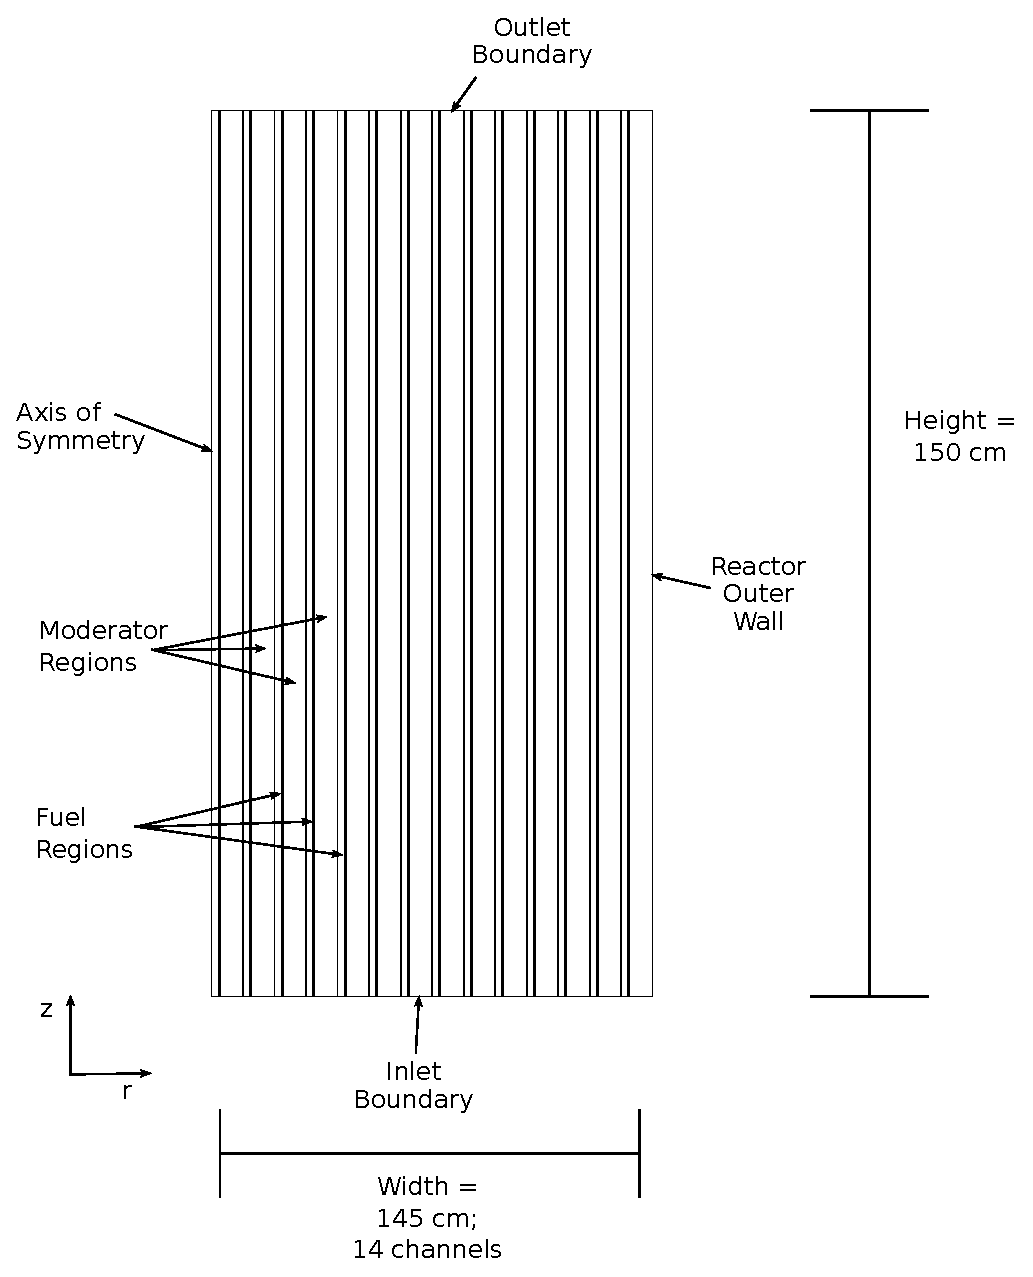
\includegraphics[width=.45\columnwidth]{msre-geometry}
	\caption{Schematic diagram of the 2-D axisymmetric \gls{MSRE} geometry
	adopted by Lindsay et al. \cite{lindsay_introduction_2018}.}
	\label{fig:msre-geometry}
\end{figure}

Figure \ref{fig:msre-geometry} shows the fuel channels and moderator regions of
the 2-D \gls{MSRE} geometry that Lindsay et al. adopted for their study.
They ran a two-group neutron diffusion model with six precursor groups and
vacuum boundary conditions on the outer boundaries governed by Equations
\ref{eq:neutron}, \ref{eq:precursor}, and \ref{eq:vacuum} shown in Section
\ref{sec:nts}. They modeled precursor drift due to fuel salt flow by imposing
fixed uniform flow upwards through the fuel channels shown in Figure
\ref{fig:msre-geometry}. Their thermal-hydraulics model employed a
governing equation for temperature in the fuel salt equivalent to Equation
\ref{eq:temp} with fixed uniform flows while imposing a cosine-shaped heat
source term representing heat dissipation from gamma and neutron irradiation in
the graphite moderator region. In addition, all governing equations were fully
coupled and solved simultaneously as a single system of equations with implicit
Euler timestepping to accurately and efficiently resolve the strong coupling
expected between the neutronics and temperature.

\begin{figure}[htb!]
	\centering
	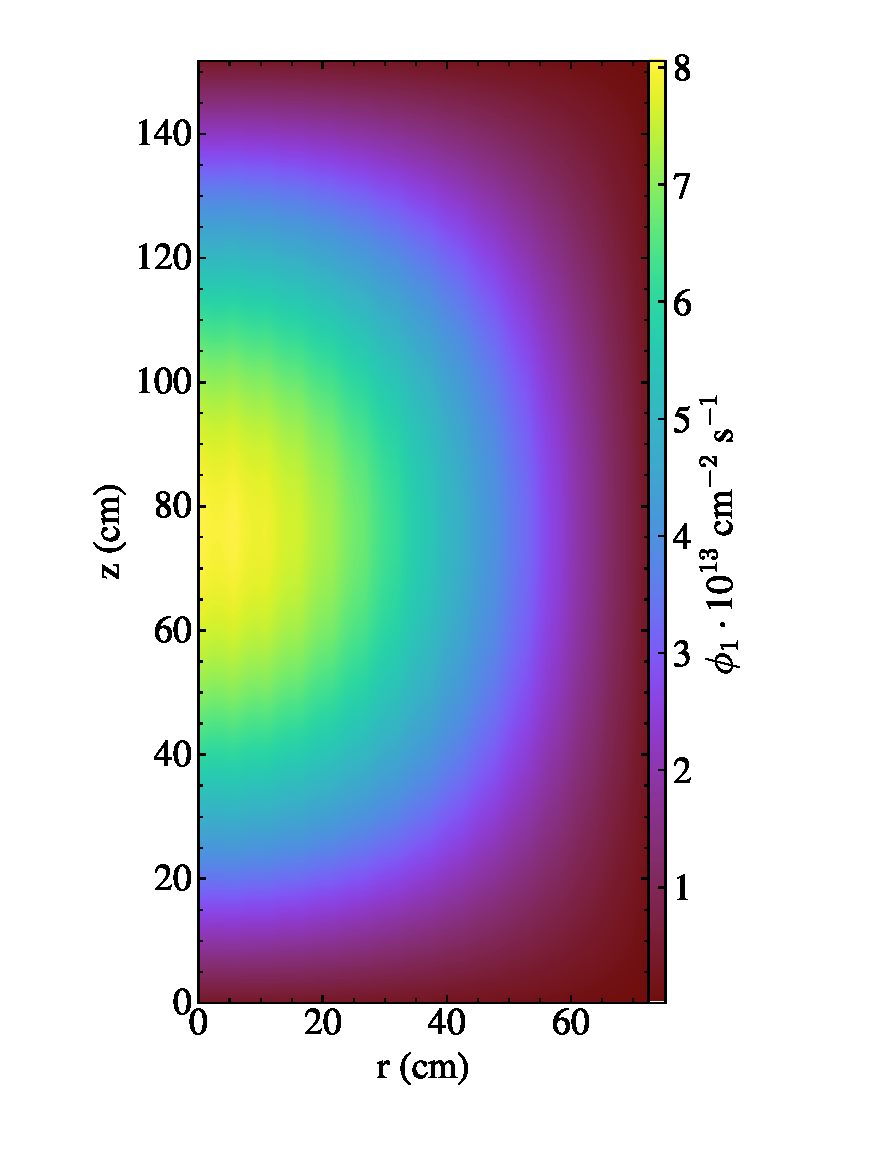
\includegraphics[width=.45\columnwidth]{2d_gamma_heating_group1}
	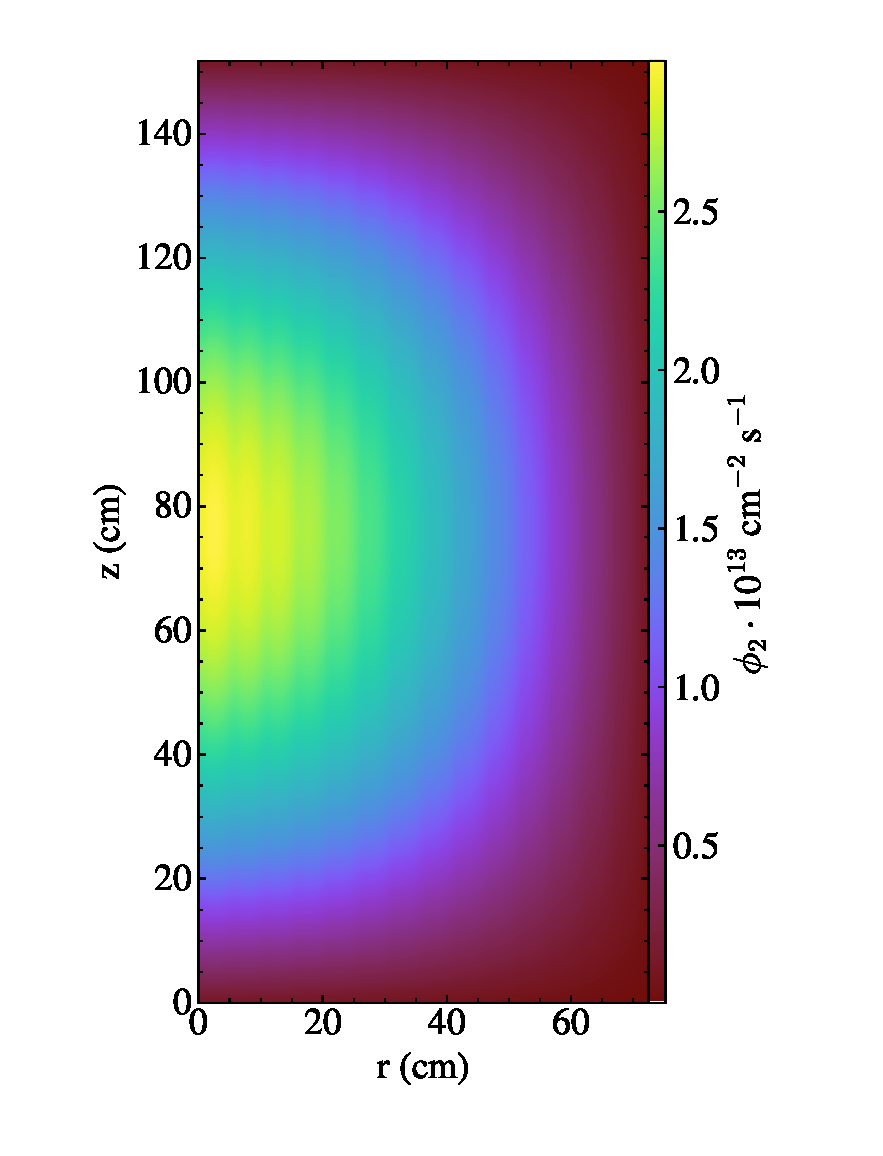
\includegraphics[width=.45\columnwidth]{2d_gamma_heating_group2}
	\caption{Neutron group 1 and 2 fluxes in the 2-D axisymmetric \gls{MSRE}
	model from Lindsay et al. \cite{lindsay_introduction_2018}.}
	\label{fig:msre-flux}
\end{figure}

\begin{figure}[htb!]
	\centering
	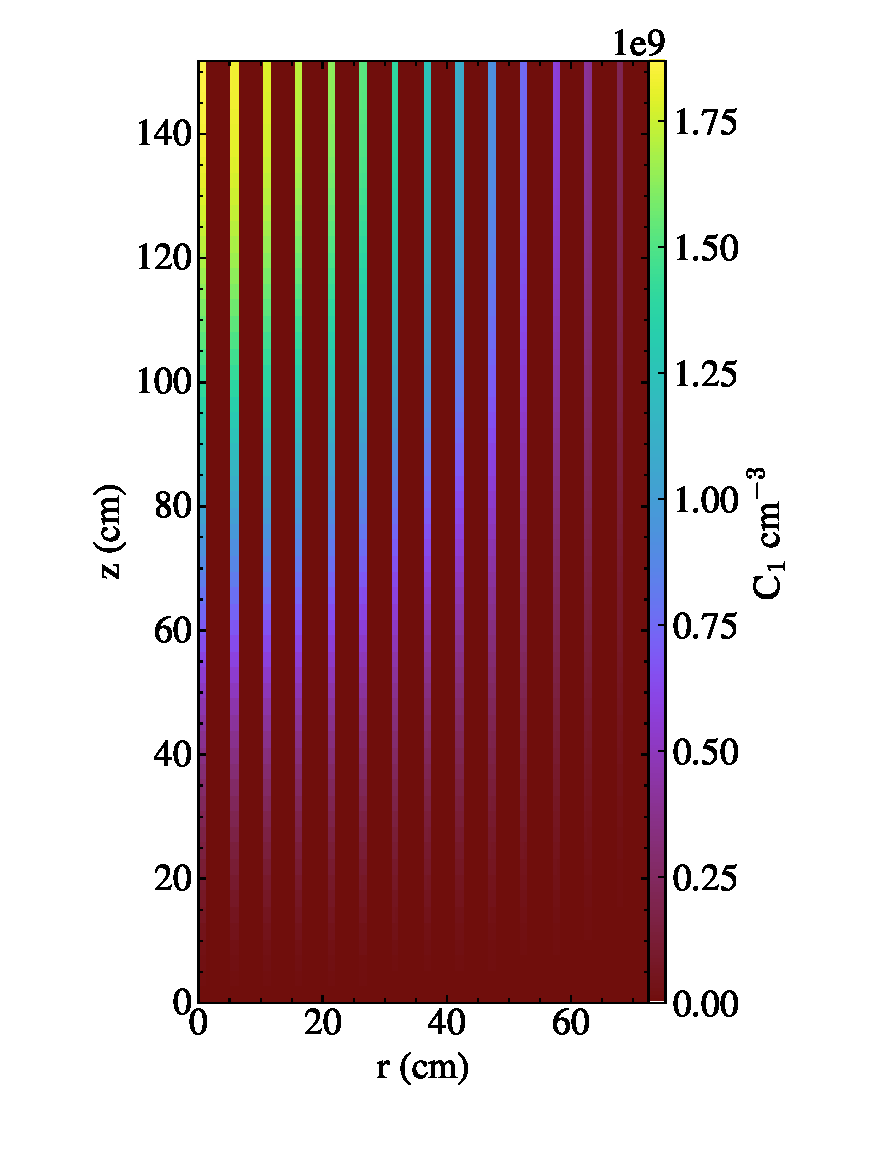
\includegraphics[width=.45\columnwidth]{2d_gamma_heating_pre1_scaled}
	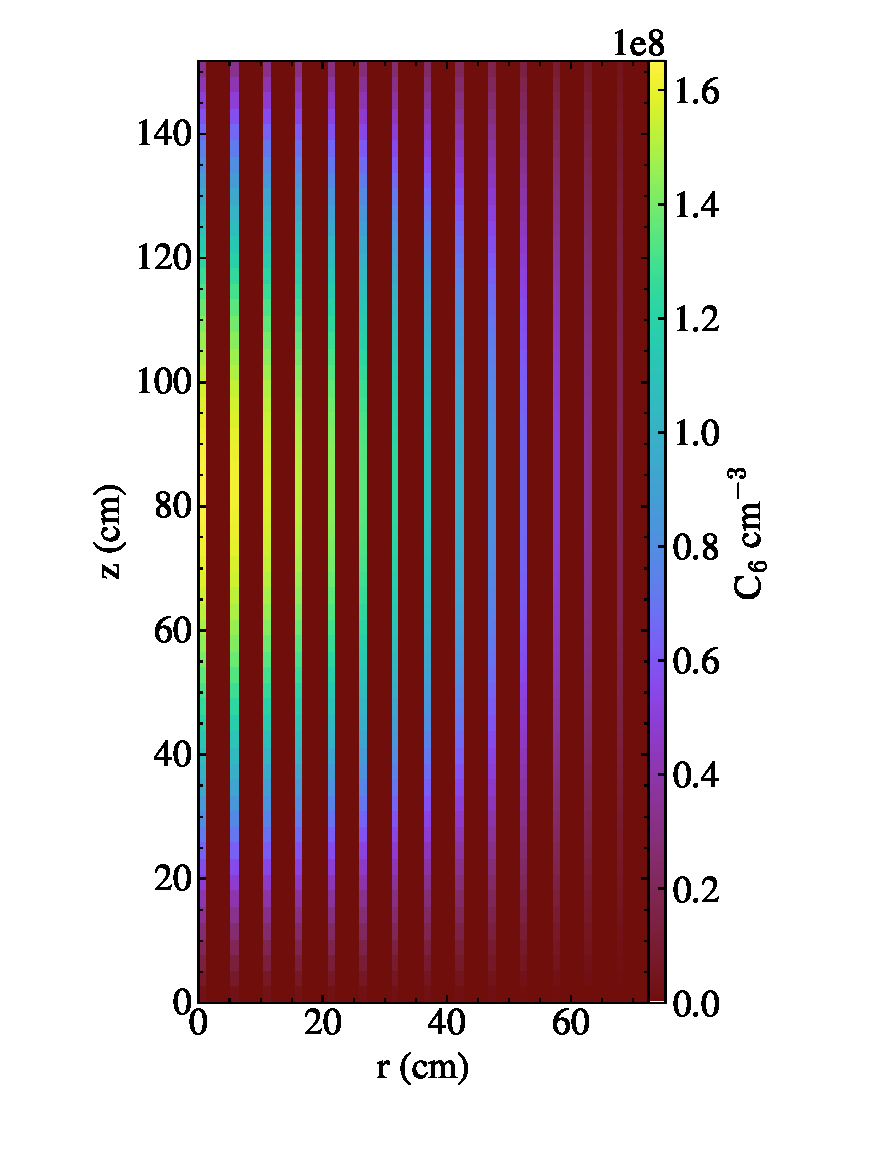
\includegraphics[width=.45\columnwidth]{2d_gamma_heating_pre6_scaled}
	\caption{Longest- and shortest-lived precursor concentrations ($\lambda =
	1.24\times 10^{-2}$s$^{-1}$ and $3.07$s${-1}$, respectively) in the 2-D
	axisymmetric \gls{MSRE} model from Lindsay et al.
	\cite{lindsay_introduction_2018}.}
	\label{fig:msre-precursor}
\end{figure}

\begin{figure}[htb!]
	\centering
	\begin{minipage}[b]{0.45\columnwidth}
	    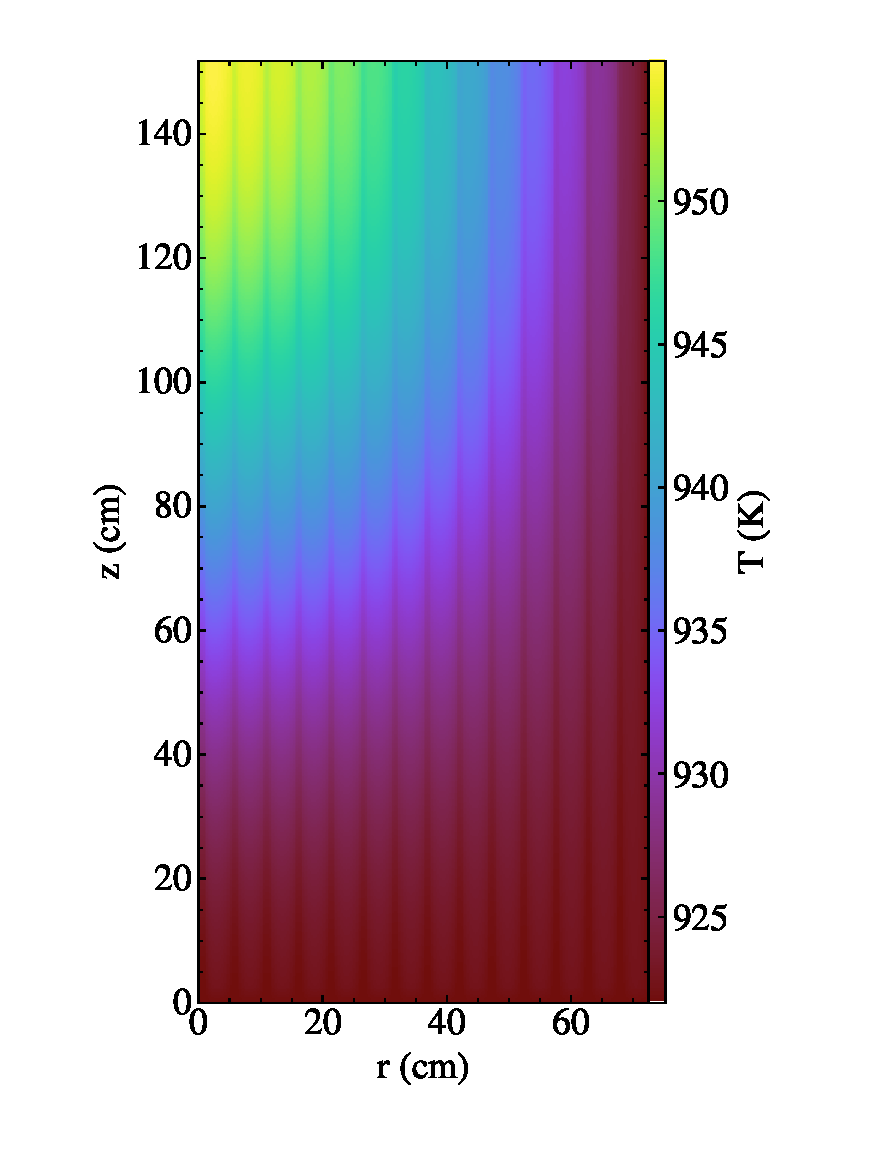
\includegraphics[width=\columnwidth]{2d_gamma_heating_temp}
	    \caption{Temperature distribution in the 2-D
	    axisymmetric \gls{MSRE} model from Lindsay et al.
	    \cite{lindsay_introduction_2018}.}
	    \label{fig:msre-temp}
	\end{minipage}
	\hfill
	\begin{minipage}[b]{0.45\columnwidth}
	    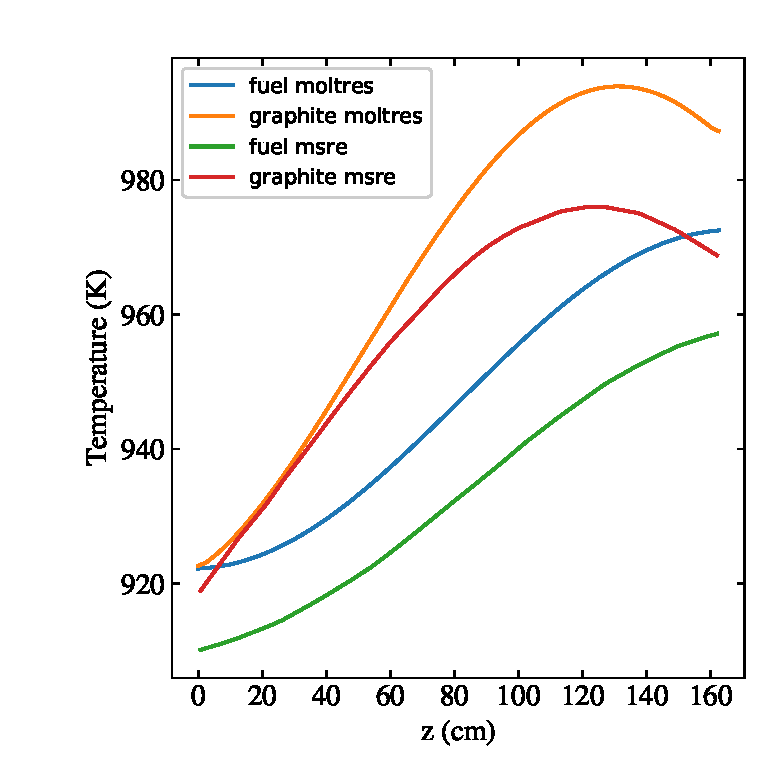
\includegraphics[width=\columnwidth]{combined_msre_moltres_axial_temps}
	    \caption{Moltres \cite{lindsay_introduction_2018} and \gls{ORNL}
	    \gls{MSRE} \cite{briggs_molten-salt_1964} axial temperature
	    distributions in the hottest fuel channel and adjacent graphite.}
	    \label{fig:msre-temp-plot}
	\end{minipage}
\end{figure}

Figure \ref{fig:msre-flux} shows the fast and thermal neutron fluxes
corresponding to group 1 and 2 in the 2-D \gls{MSRE} model. As expected, the
fluxes exhibit general cosine shapes in the axial and radial directions. We
also observe minor oscillations in the radial direction coinciding with the
regular fuel and moderator lattice. The fuel regions favor the fast flux, while
the moderator regions favor the thermal flux.

Figure \ref{fig:msre-precursor}
shows the longest- and shortest-lived precursor concentrations in the fuel
channels. With a long half-life of 55.9 s relative to the 6.91 s it takes for
salt to flow from bottom to top, the longest-lived precursor concentration peaks
outside the model domain. By contrast, the shortest-lived precursor
concentration closely follows the neutron fluxes' cosine shape, which
dictate where the precursors are born.

Finally, Figure \ref{fig:msre-temp}
shows the temperature distribution in the 2-D \gls{MSRE} model. The temperature
naturally peaks near the outlet due to upward advection. The moderator regions
experience hotter temperatures than the fuel regions due to radiative heating
and the relative inefficiency of heat conduction in the graphite compared to
advection in the fuel salt.

\begin{figure}[htb!]
	\centering
	\begin{subfigure}[h]{0.45\columnwidth}
	    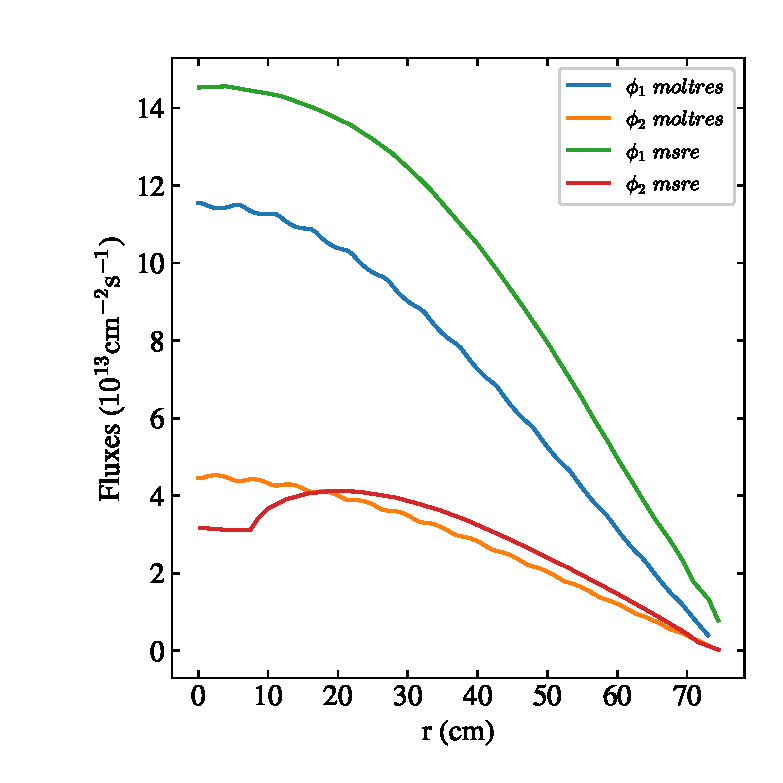
\includegraphics[width=\columnwidth]{combined_msre_moltres_radial}
	    \caption{Radial fluxes at reactor half-height.}
	    \label{fig:msre-flux-radial}
	\end{subfigure}
	\hfill
	\begin{subfigure}[h]{0.45\columnwidth}
	    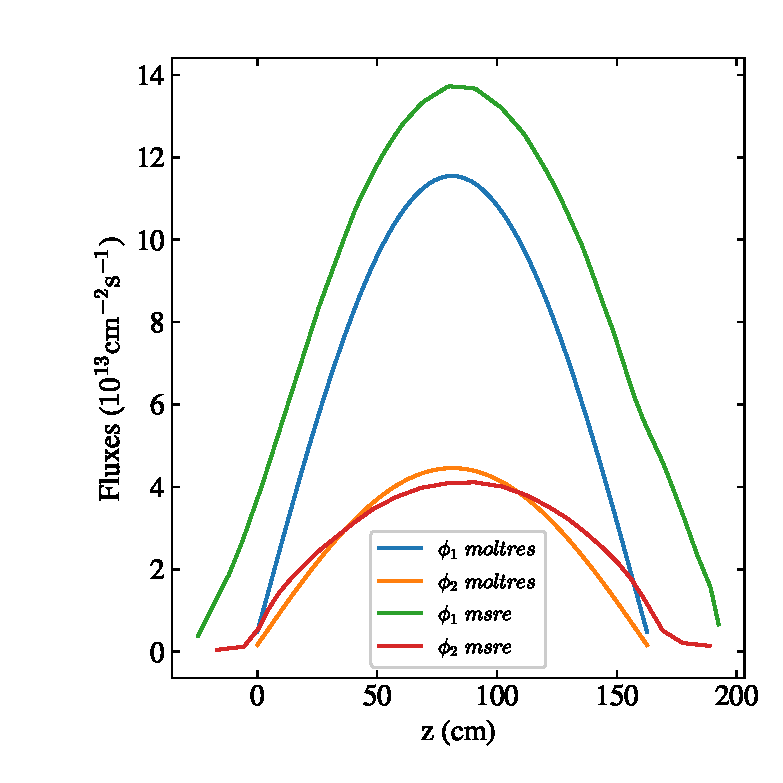
\includegraphics[width=\columnwidth]{combined_msre_moltres_axial}
	    \caption{Axial fluxes along the core centerline ($r=0$ cm).}
	    \label{fig:msre-flux-axial}
	\end{subfigure}
	\caption{The fast and thermal fluxes from
	Moltres \cite{lindsay_introduction_2018} and the \gls{ORNL} \gls{MSRE}
	design calculations \cite{briggs_molten-salt_1964}.}
\end{figure}

The corresponding neutronics and thermal-hydraulics results from their 3-D model
show good qualitative agreement with the 2-D results. Given the lack of
\gls{MSR} experimental data, they compared their 2-D model results with
\gls{MSRE} design calculations performed using legacy software in 1963-1964 at
\gls{ORNL}. Their neutron flux and temperature distribution results showed good
qualitative agreement with \gls{ORNL} data. The authors attributed
discrepancies to the following differences in the two modeling approaches: the
absence of axial heat conduction and the use of 32 neutron groups in the
\gls{ORNL} calculations, and the exclusion of control rod thimbles in the
Moltres calculations.

\paragraph{Critical Assessment} \label{sec:msre-critique}

Lindsay et al.'s work illustrated early development efforts for neutronics and thermal-hydraulics
models in Moltres. It demonstrated, along with advanced capabilities from the \gls{MOOSE}
framework, fully-coupled simulations of the \gls{MSRE} with implicit timestepping. The
decent qualitative agreement observed between Moltres and the \gls{ORNL}
\gls{MSRE} calculations proved that Moltres could simulate
\glspl{MSR} under some simplifying assumptions.

On the other hand, significant improvements could be made to Moltres to better
model multiphysics phenomena in \glspl{MSR}. For instance, replacing the
fixed uniform salt flow with a proper flow profile governed by fluid flow
equations would accurately capture precursor and temperature advection.
Temperature advection has a particularly large impact on the temperature
distribution in the fuel salt since molten salts generally have large Prandtl
numbers, which measure the ratio of convective to conductive heat transfer.
The flow-modeling feature would be of even greater importance when modeling
pool-type \glspl{MSR}, which consist of a single large fuel salt region in the
reactor core.

Another essential feature for modeling \glspl{MSR}, which was already under
development at the time of publication, is a precursor loop
system to recirculate precursors back into the core. While some precursors
decay outside the core, others survive long enough to recirculate back into the
core. The loop system would provide a more accurate estimate of the delayed
neutron fraction instead of discarding all precursors that flowed out of
the core. In transient simulations involving sudden increases in the neutron
flux, precursors recirculating into the core can induce observable jumps and
dips in the power output due to the associated reactivity insertion from the
delayed neutrons.

Moltres would also benefit from a decay heat model which Lindsay
et al. mentioned in their work \cite{lindsay_introduction_2018},
especially for transient accident analyses. While decay heat from fission
product decays represents a small fraction ($\sim5\%$) of total power output,
this heat source can be significant in unprotected loss of flow or loss of
secondary cooling accidents. Therefore, understanding residual heat generation
from fission product decays in \gls{MSR} is essential in preventing further
structural failure after an accident.

Specific to reactor physics modeling, Moltres also requires an accurate method for modeling
control rods. As observed in Figure \ref{fig:msre-flux}, the omission of control rods led to
significant discrepancies in the thermal flux distribution. However, developing control rod
modeling capability in Moltres is nontrivial given that neutron diffusion theory performs poorly
within highly neutron-absorbing regions.

Lastly, the authors recognized two other avenues for future work: further \gls{VV} of Moltres'
capabilities by comparison
with more detailed experimental data and other modern \gls{MSR} modeling
efforts; and the study of transient simulation cases such as control rod
ejection, single channel blockage, loss of flow, and loss of secondary cooling.

\subsubsection{Advancements in Moltres and Transient Simulations of the MSFR}
\label{sec:msfr}

This section follows my previous work for my Master's degree in \textit{Advancement and
Verification of Moltres for Molten Salt Reactor Safety Analysis} \cite{park_advancement_2020},
which I shall refer to as ``this work'' in this subsection.

In many ways, this work represents a continuation of the work by Lindsay et al.
\cite{lindsay_introduction_2018} in developing Moltres as an \gls{MSR}
simulation tool. New features introduced include coupling the existing
neutronics and temperature equations to incompressible Navier-Stokes equations
to model flow dynamics, the precursor loop system, and the decay heat model.
I later demonstrated these features through steady-state and transient
simulations of a 2-D axisymmetric \gls{MSFR} model.

Moltres couples natively with the \texttt{Navier-Stokes} module in \gls{MOOSE} for
incompressible flow modeling capabilities. Section \ref{sec:th} describes the governing equations
for incompressible flow and temperature advection-diffusion.
The precursor loop model was developed to model
precursor recirculation into the core. The precursor loop system leverages
the \texttt{MultiApp} system in \gls{MOOSE} to couple a 1-D pipe model to the
core to simulate precursor flow outside the core. The core and the pipe models
are coupled via inlet and outlet boundary conditions, as detailed in Section
\ref{sec:moltres-loop}. The loop system can also accommodate a pointwise heat
exchanger model with a heat removal rate as a function of time
or auxiliary variables in the Moltres simulation.

In addition, I developed a decay heat model to simulate delayed heat release
from the decay of fission products, similar to delayed neutron emission
from precursors. The decay heat model introduces decay heat groups of different
decay constants and variables representing the decay heat groups and modifies the
heat source term given by Equation \ref{eq:heat-source} to account for
the delayed heat generation. 

The number of decay heat groups depends on
the decay heat profile of the reactor after a specified period of operation.
Determining the decay heat profile requires fuel depletion calculations to
obtain the fuel composition during/after reactor operation and subsequent
calculations for the cumulative decay heat released from individual isotopes.
In this work, I cited results by Aufiero et al. \cite{aufiero_extended_2013},
who determined that three decay heat groups ($J=3$) were sufficient to
reproduce the decay heat profile of the \gls{MSFR} equilibrium fuel composition
for up to 300 seconds after shutdown with a relative error of less than 2\%.

\begin{figure}[htb!]
	\centering
	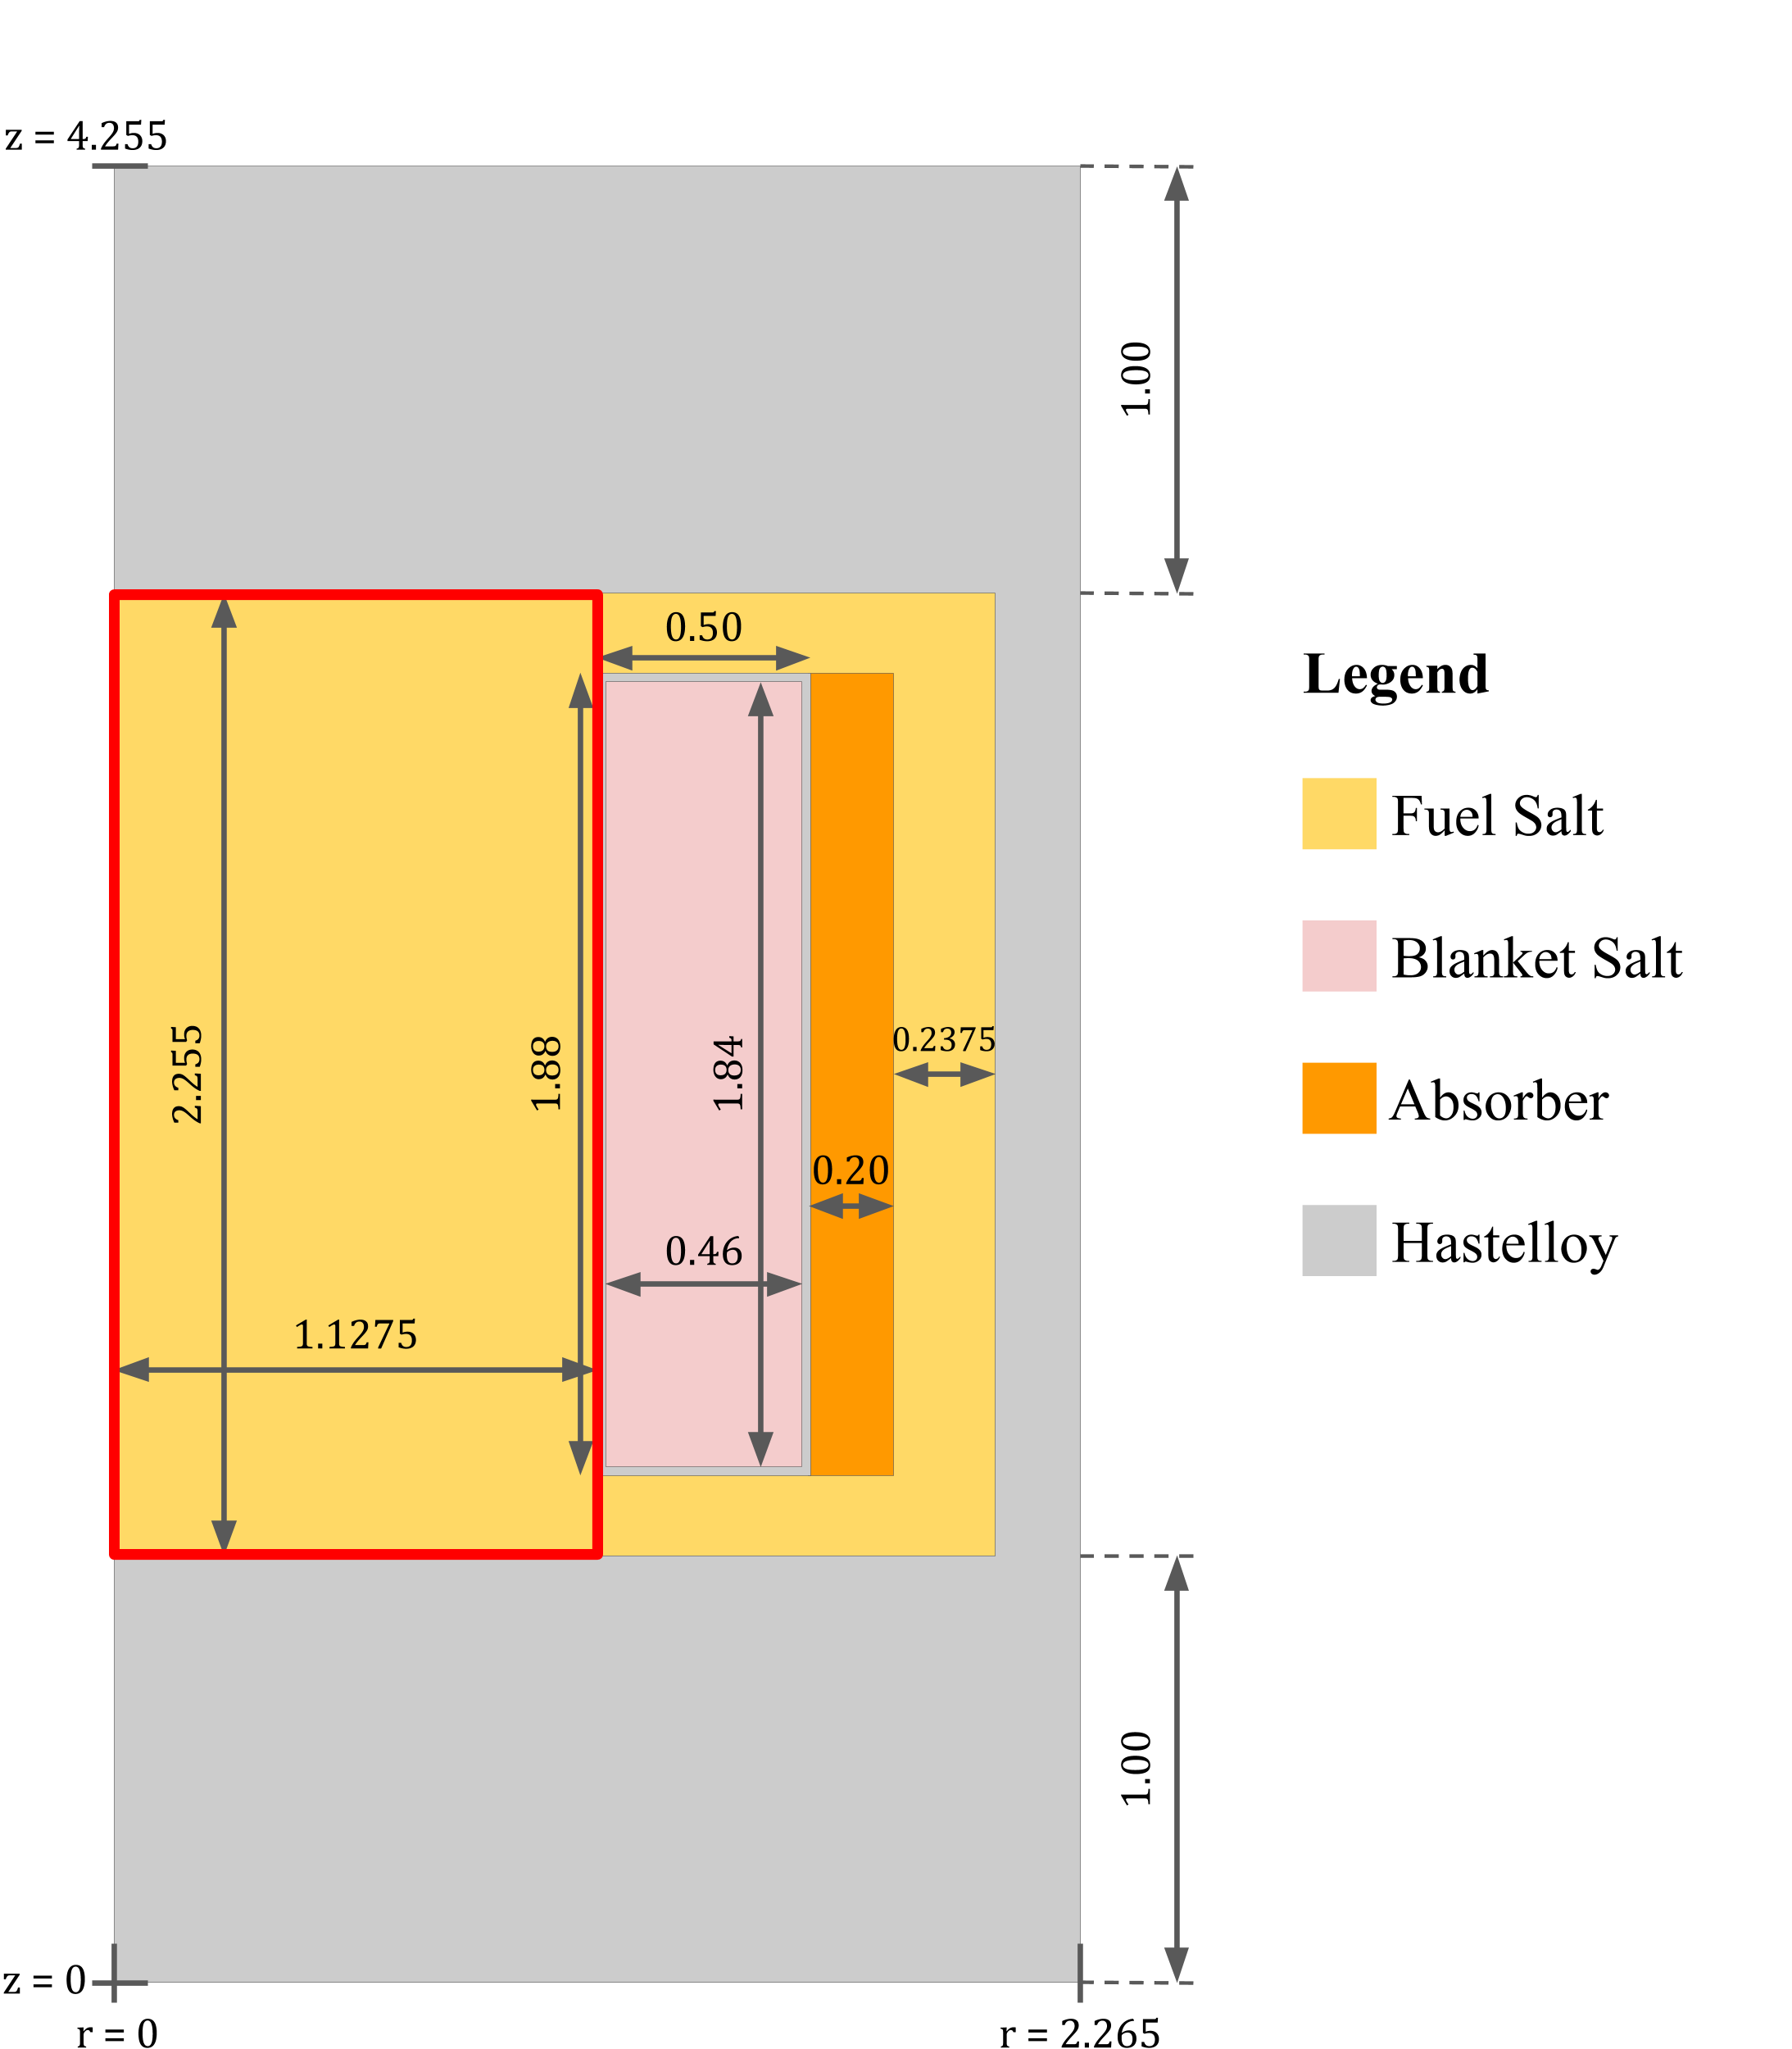
\includegraphics[width=.55\columnwidth]{central-core-legend}
	\caption{Schematic diagram of the 2-D axisymmetric \gls{MSFR} model with
	the core region enclosed by the red box \cite{park_advancement_2020}.}
	\label{fig:msfr-geometry}
\end{figure}

For the verification and demonstration of the capabilities introduced in this
work, I ran coupled steady-state and unprotected accident transient
simulations of the \gls{MSFR} and compared the results with published results
by Fiorina et al. \cite{fiorina_modelling_2014} and Aufiero et al.
\cite{aufiero_development_2014}. In this section, the PoliMi and TU Delft models
refer to two sets of results published by Fiorina et al. I compensated for
the lack of a turbulence model in Moltres by imposing a fixed turbulent
viscosity of 40 Pa$\cdot$s in addition to the molecular viscosity $\mu$ in
Equation \ref{eq:momemtum}. Figure \ref{fig:msfr-geometry} shows the 2-D
axisymmetric \gls{MSFR} model with the core region indicated with the red box,
while the rest of the fuel region was modeled with the 1-D loop system. Fuel
salt flows into the core region from the inlet at the bottom-right corner and
out through the outlet at the top-right corner.

\begin{figure}[htb!]
    \centering
    \begin{subfigure}[t]{.35\textwidth}
        \centering
        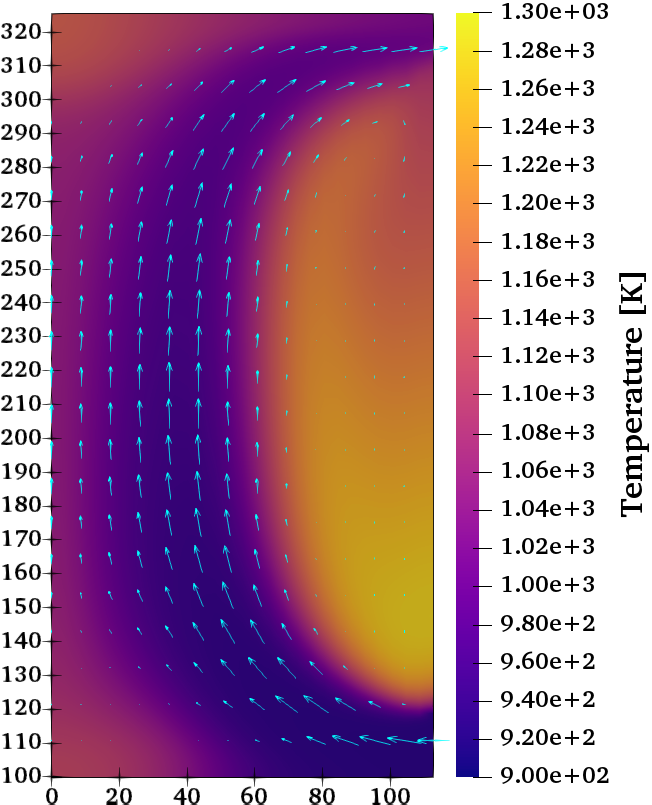
\includegraphics[width=\textwidth]{flow-temp-plasma}
    \end{subfigure}
    \hfill
    \begin{subfigure}[t]{.625\textwidth}
        \centering
        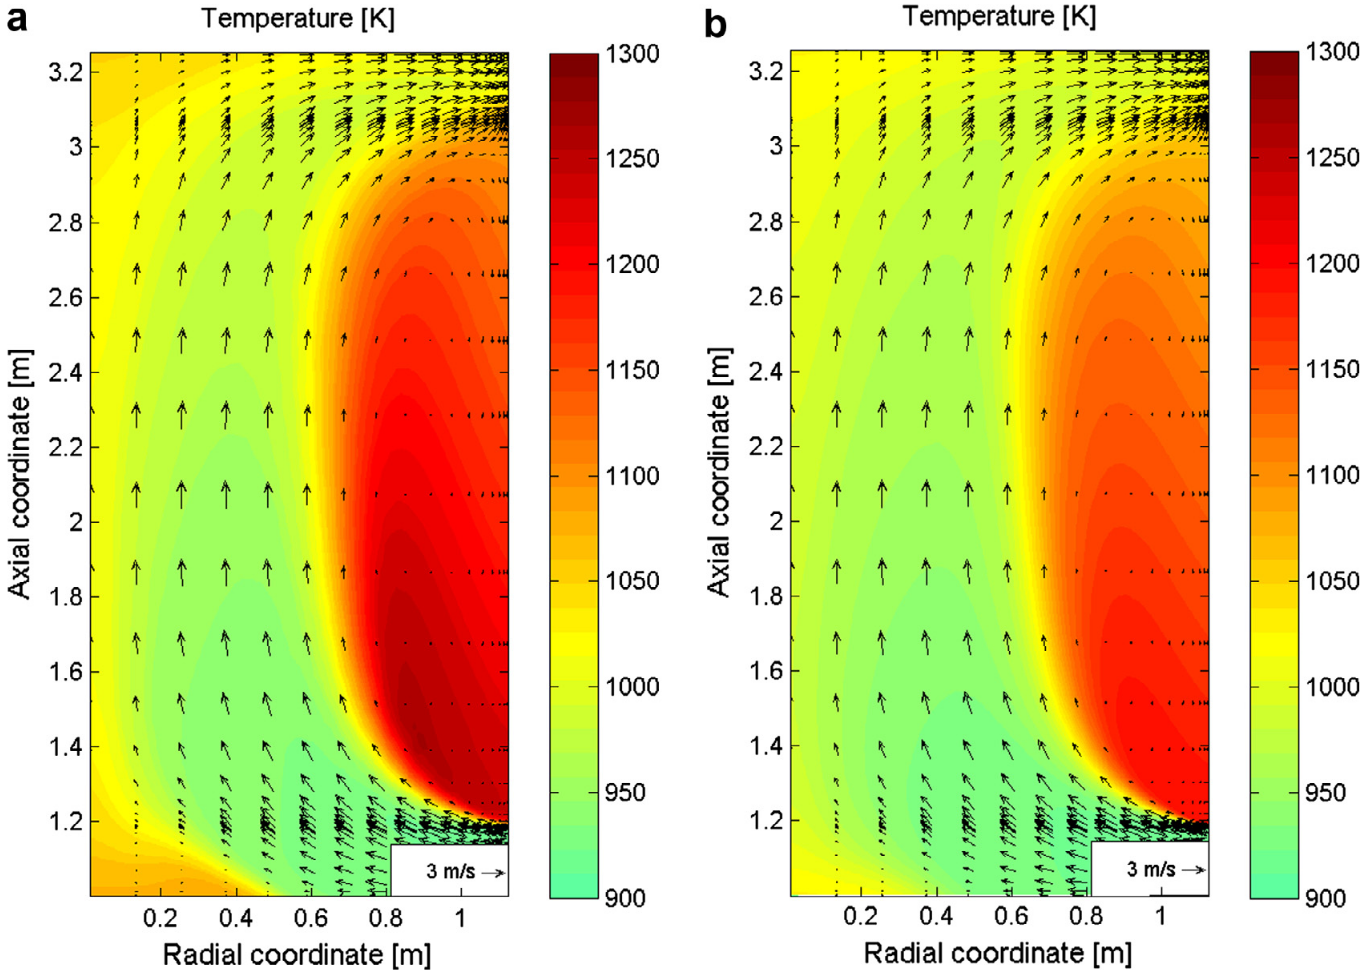
\includegraphics[width=\textwidth]{flow-temp-fiorina}
    \end{subfigure}
    \caption{Temperature and velocity fields in the core from Moltres
    (left), PoliMi (center), and TU Delft (right) models. The colors represent
    temperature according to the respective color bars and the arrows
    represent velocity fields. \cite{park_advancement_2020}}
    \label{fig:flow-temp}
\end{figure}

Figure \ref{fig:flow-temp} shows the core steady-state temperature and velocity
fields from the Moltres, PoliMi, and TU Delft models. The Moltres
model showed
good qualitative agreement with the PoliMi and TU Delft models since the plots
show similar flow and hotspot features in all three models. The salt flow
follows a parabolic path from the inlet to the outlet. A large
recirculation region formed near the right wall while the top and bottom
regions along the central axis experience relatively stagnant flow compared to
the main salt flow stream. The temperature hotspots coincide with the regions of
recirculation and stagnation because convection is the dominant heat transfer
mechanism. Maximum temperatures are observed near the bottom of the
recirculation zones; the Moltres model reports 1275 K, which is closer to the
PoliMi model ($\sim1300$ K) than the TU Delft model ($\sim1200$ K). Thus, the
incompressible flow model in Moltres performed well in reproducing the
thermal-hydraulic profiles of the \gls{MSFR} under steady-state conditions
despite the fixed turbulent viscosity assumption.

\begin{figure}[b!]
    \centering
    \begin{subfigure}[t]{.30\textwidth}
        \centering
        \vspace{.9cm}
        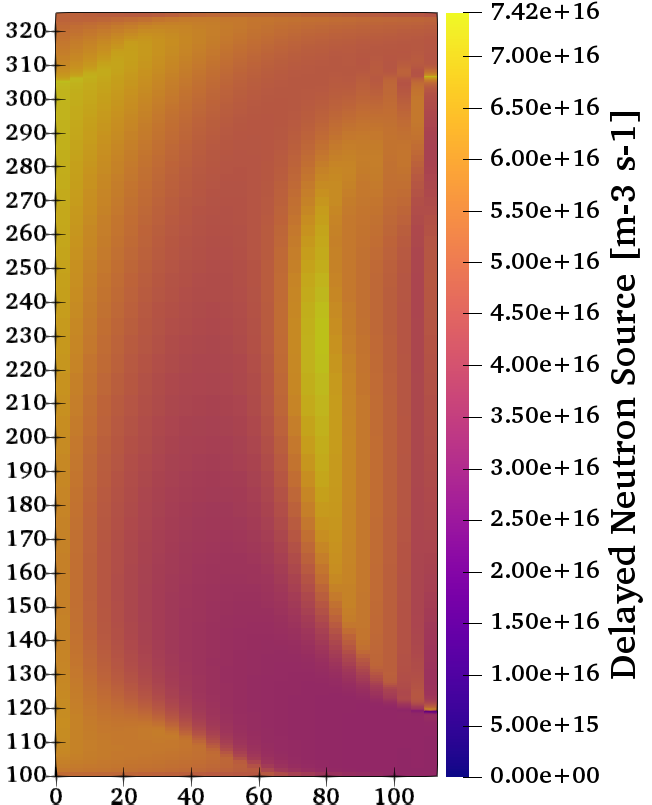
\includegraphics[width=\textwidth]{pre}
    \end{subfigure}
    \begin{subfigure}[t]{.69\textwidth}
        \centering
        \vspace{0pt}
        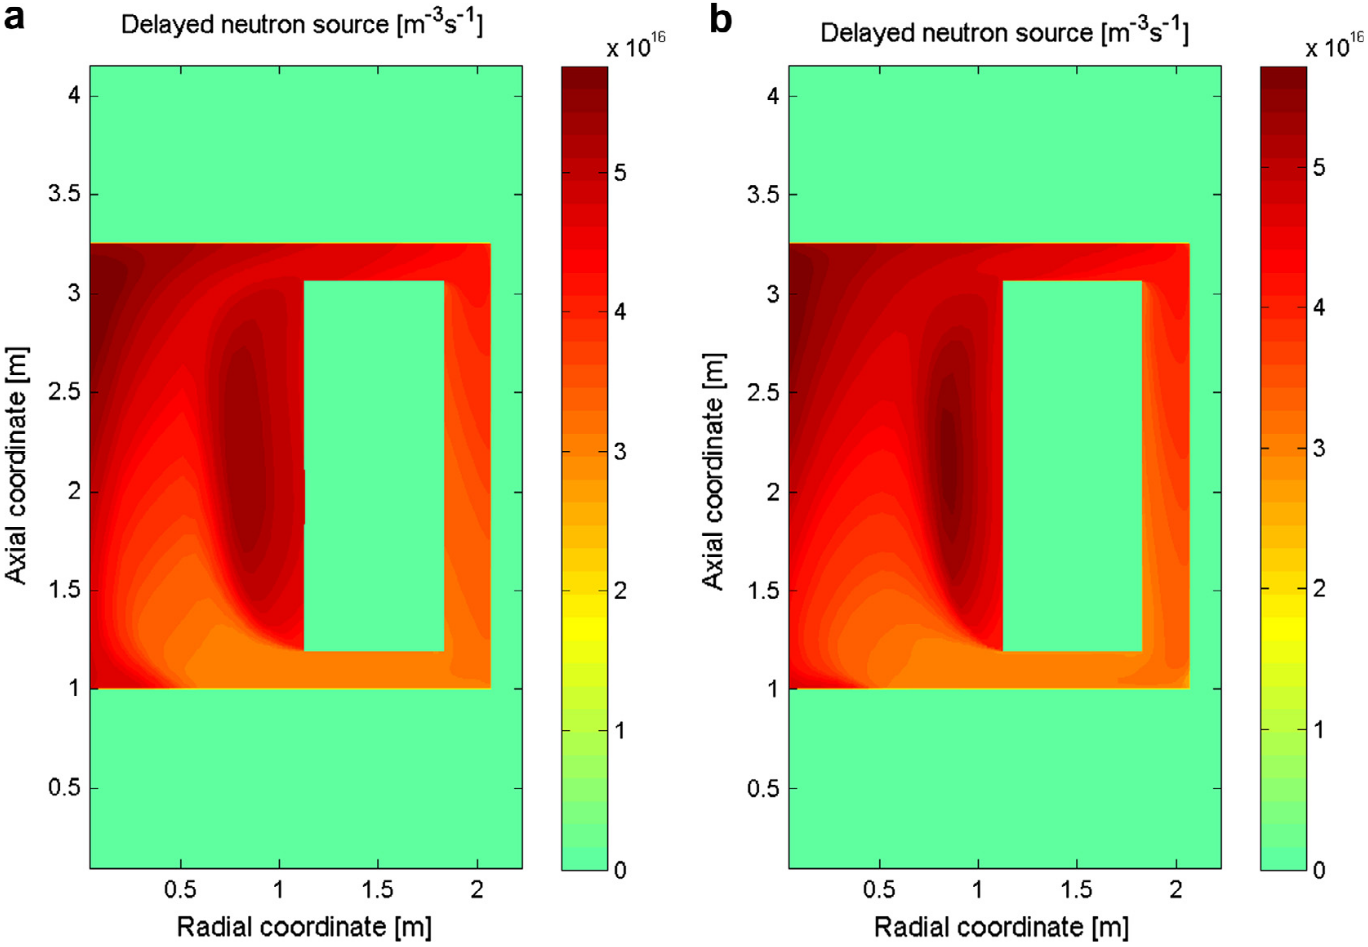
\includegraphics[width=\textwidth]{fiorina-pre}
    \end{subfigure}
    \caption{Total delayed neutron source distribution in the core from the
    Moltres (left), PoliMi (center), and TU Delft (right) models.}
    \label{fig:pre}
\end{figure}

Moltres reported a peak total neutron flux of $9.80 \times 10^{15}$
cm$^{-2}\cdot$s$^{-1}$, which is close to the 8.6 and 9.0 $\times 10^{15}$
cm$^{-2}\cdot$s$^{-1}$ values reported by Fiorina et al.
\cite{fiorina_molten_2013} and \cite{aufiero_development_2014}. However, the
delayed neutron source distribution from the Moltres model exhibits some
differences compared to the PoliMi and TU Delft models, as shown in Figure
\ref{fig:pre}. The Moltres model retains fewer precursors than the other two
models, resulting in a higher 44.16\% out-of-core delayed neutron emissions
compared with the 34.80\% and 34.85\% from the other models
\cite{park_advancement_2020}. Therefore, the incompressible flow model with
constant turbulent viscosity fell short of accurately capturing precursor
drift in the \gls{MSFR}.

\begin{figure}[htb]
    \centering
    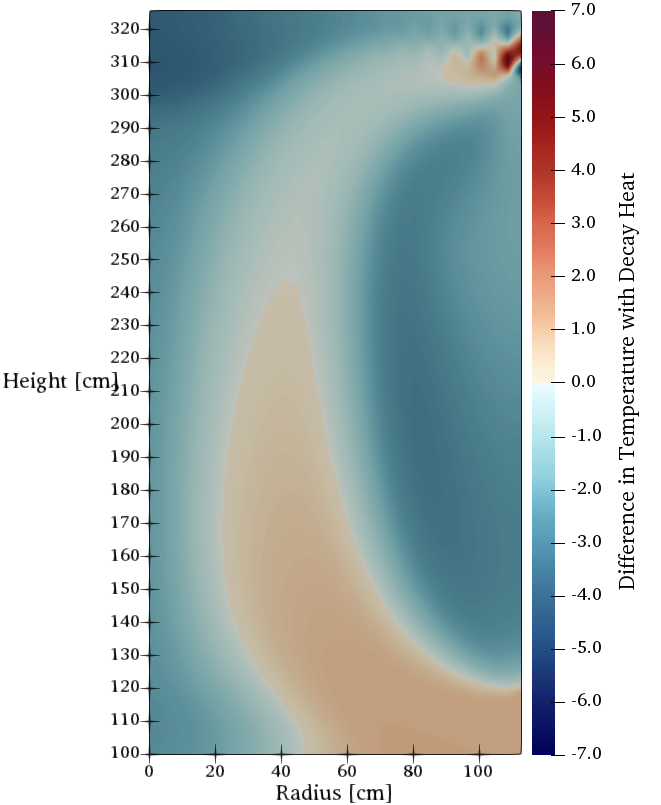
\includegraphics[width=.5\textwidth]{decay-heat-temp}
    \caption{Difference in core temperatures at steady-state with decay heat
    relative to the result without decay heat (Figure \ref{fig:flow-temp}).}
    \label{fig:decayheattemp}
\end{figure}

This work also compared steady-state temperature distributions with and without
the decay heat model. As expected, the decay heat model effectively flattens
the heat source distribution, reducing the maximum
temperatures and increasing the minimum temperatures observed in the model.
Figure \ref{fig:decayheattemp} shows a decrease in temperature in the hotspot
regions and an increase in temperature near the inlet, the coolest
region in the core.

For the transient studies, this work considered unprotected reactivity
insertion, loss-of-heat-sink, loss-of-flow, and pump-overspeed accidents. The
term ``unprotected'' signifies accident scenarios without reactor SCRAM.
Moltres reproduced similar trends observed in the PoliMi and TU Delft
models for the reactivity insertion and loss-of-heat-sink scenarios. For
instance, Figure \ref{fig:200pcmheat} shows the power output response of the
three models following a 200 pcm step reactivity insertion. The lower peak from
the Moltres model is attributed to the stronger negative fuel temperature
reactivity feedback coefficient of $-7.184$ pcm$\cdot$K$^{-1}$ compared to
approximately $-6.5$ pcm$\cdot$K$^{-1}$ for the PoliMi and TU Delft models.

\begin{figure}[htb!]
    \centering
    \begin{minipage}[b]{.49\textwidth}
      \centering
      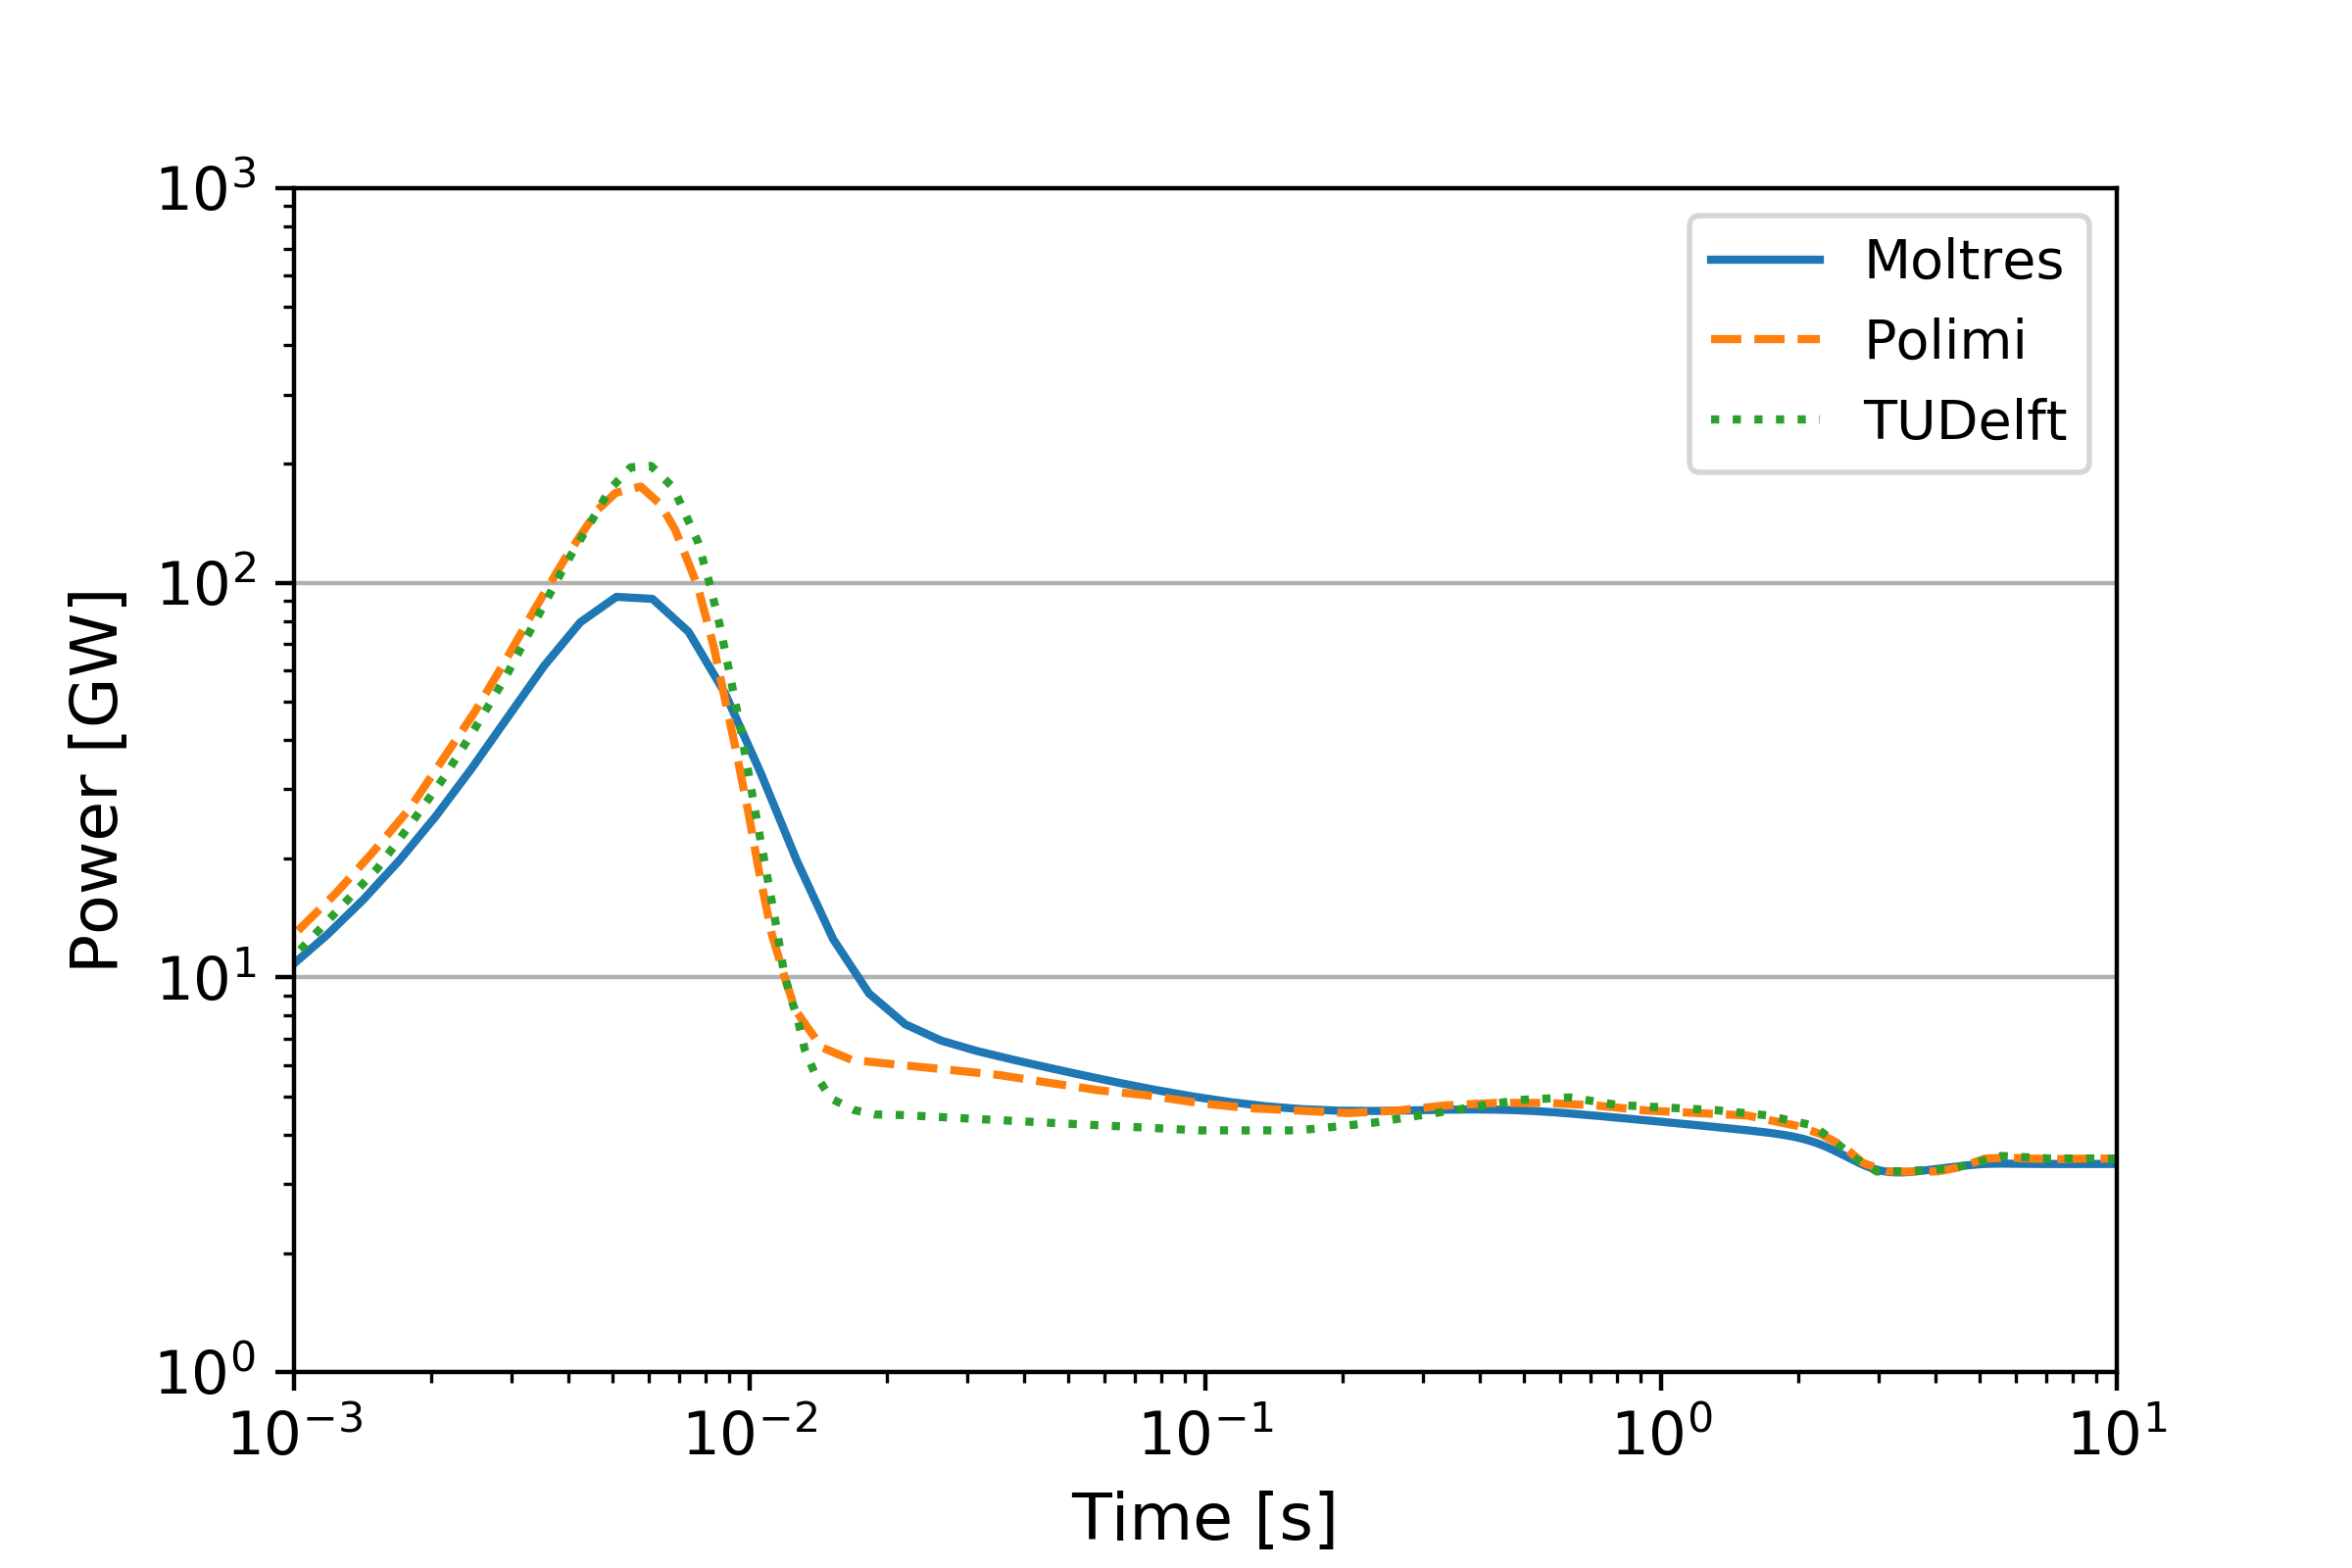
\includegraphics[width=\textwidth]{200pcm-heat}
      \caption{Power output following a 200 pcm step-wise unprotected reactivity
        insertion in the Moltres, PoliMi, and
        TU Delft models \cite{fiorina_modelling_2014}.}
      \label{fig:200pcmheat}
    \end{minipage}
    \hfill
    \begin{minipage}[b]{.49\textwidth}
      \centering
      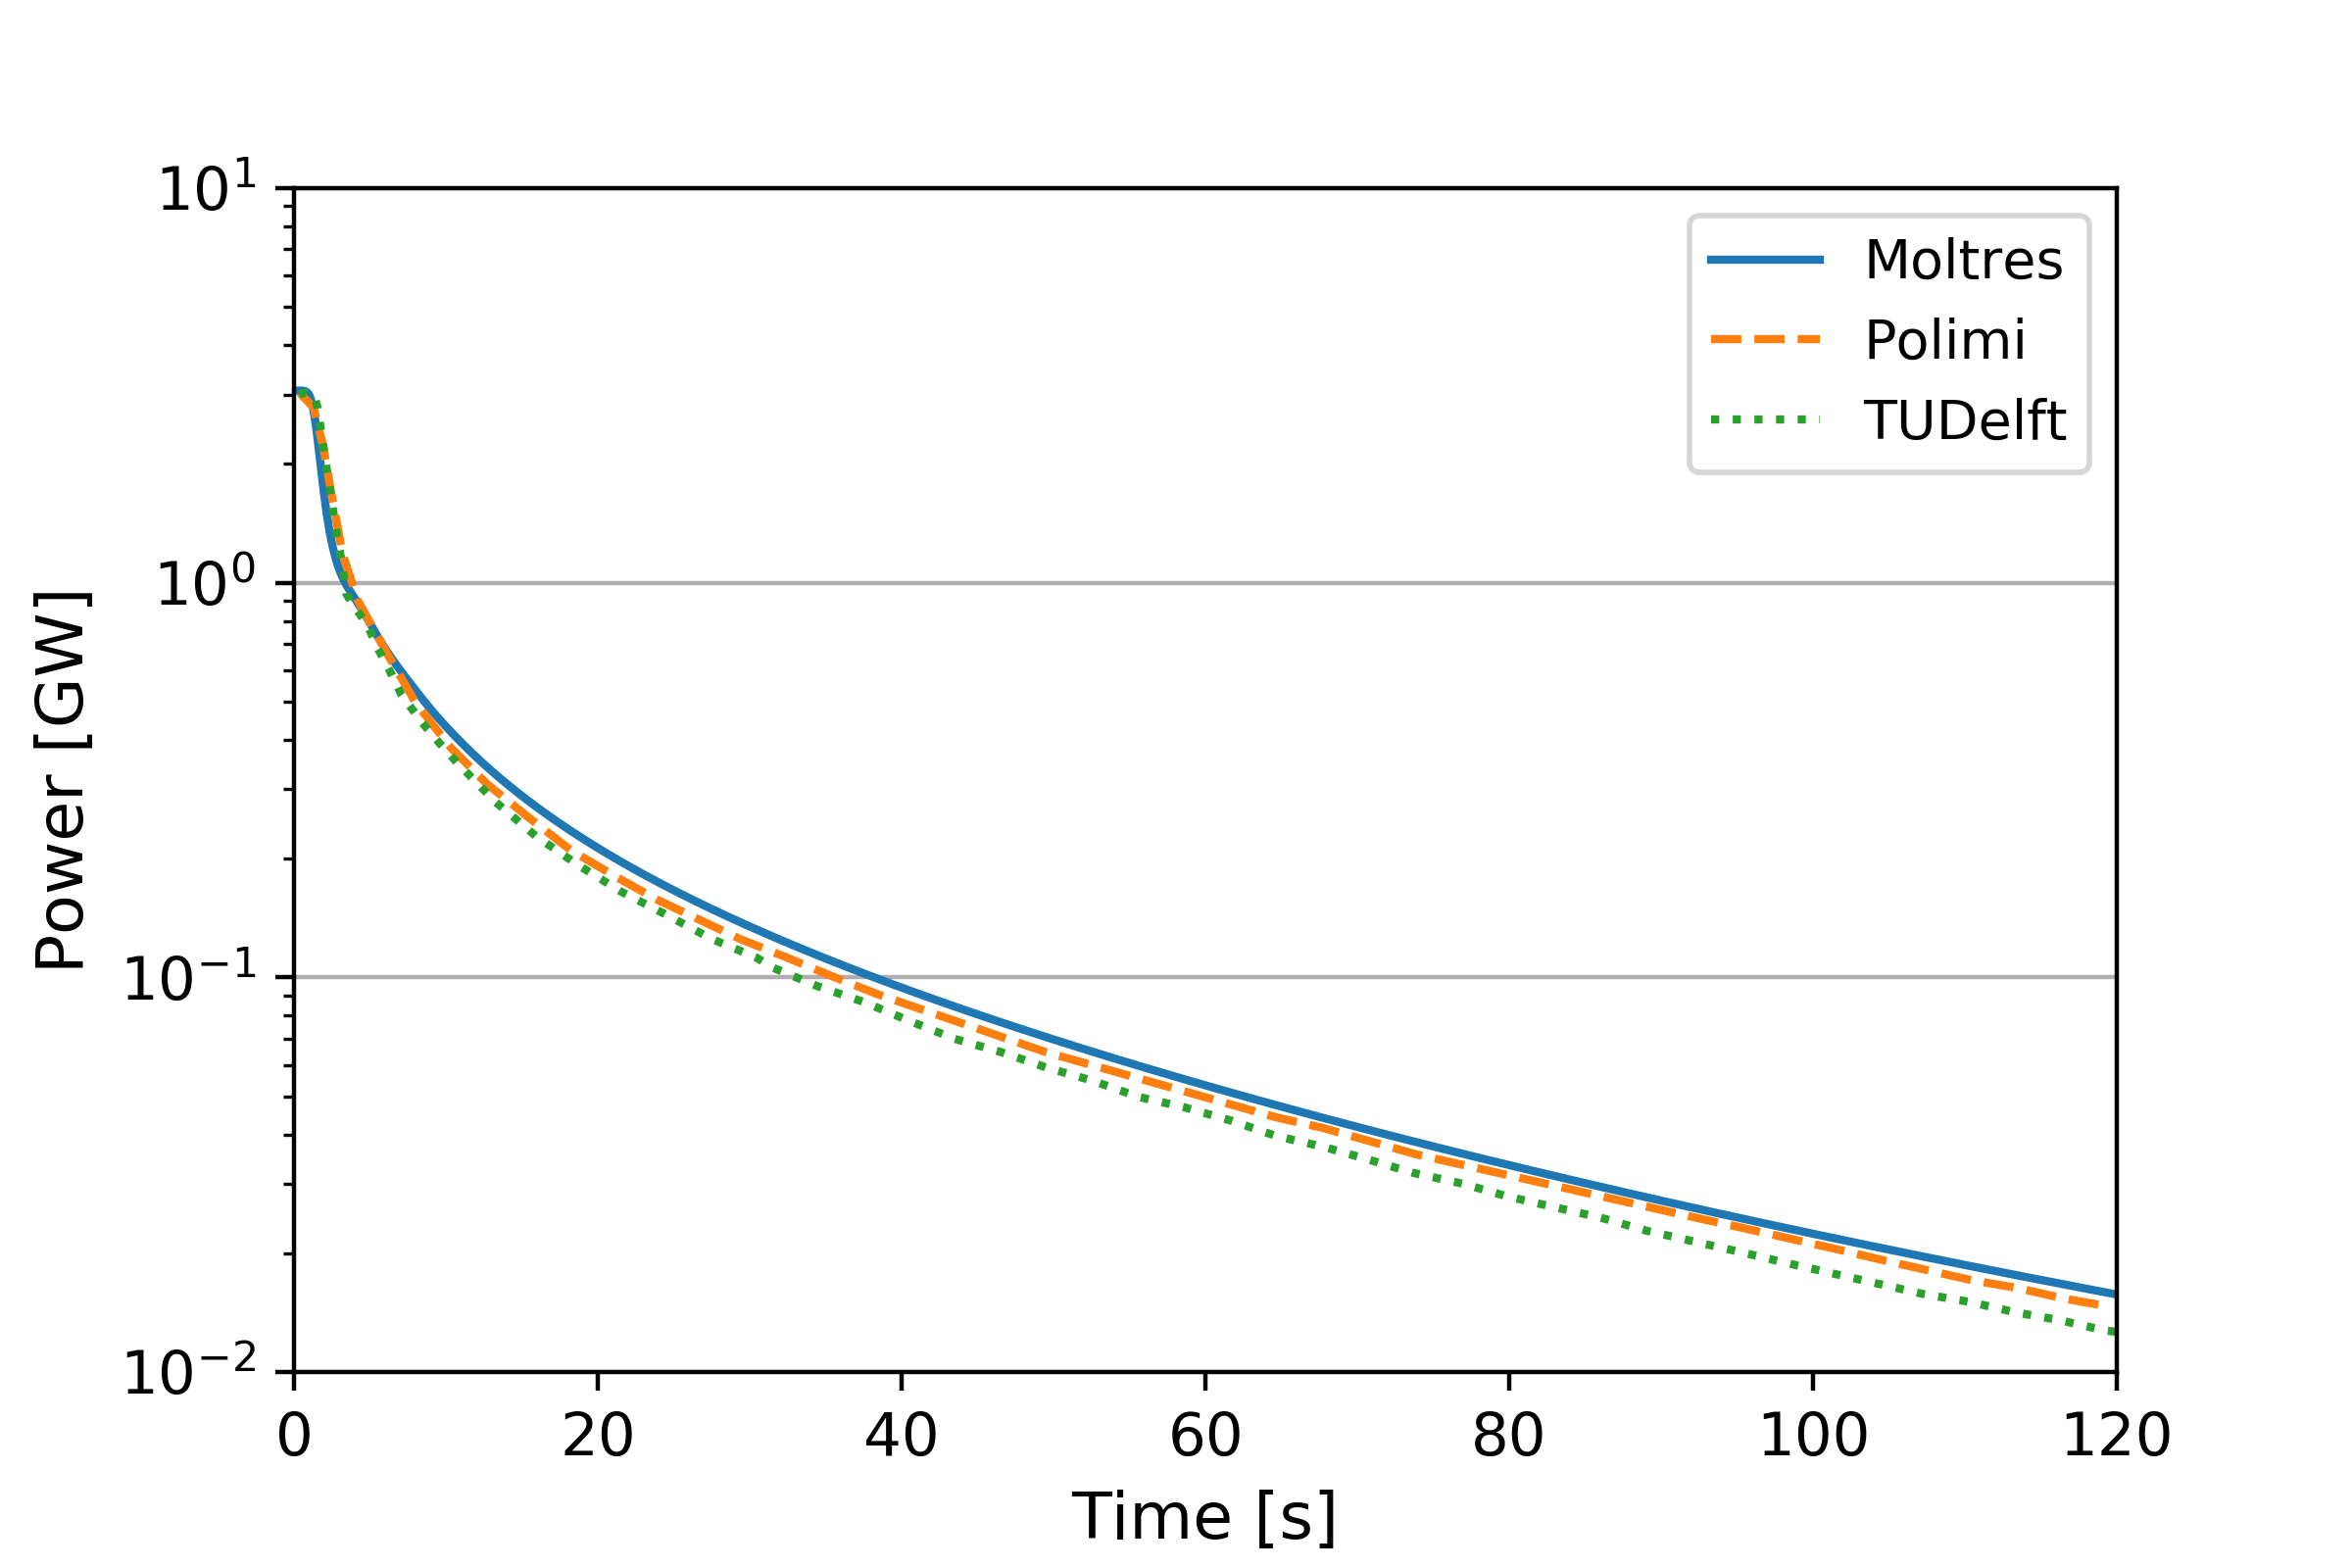
\includegraphics[width=\textwidth]{lohs-heat}
      \caption{Power output during
        an unprotected loss of heat sink transient in the Moltres, PoliMi, and
        TU Delft models \cite{fiorina_modelling_2014} without decay heat.}
      \label{fig:lohsheat}
    \end{minipage}
\end{figure}

The loss-of-heat-sink transients were performed with and without the decay heat
model because the TU Delft model did not possess this capability. As shown in
Figure \ref{fig:lohsheat}, without decay heat, all three models reported
similar power output responses following the loss of cooling through the heat
exchanger modeled as an exponential decrease in heat removal rate with a time
constant of 1 s. As prompt heat generation decreases due to rising core
temperatures and the negative temperature reactivity feedback, decay heat
becomes a significant heat source. We observe this in Figure
\ref{fig:moltresdecaypower}, which shows decay heat output overtaking prompt
heat output 34 s into the accident scenario. With the decay heat model, the
Moltres model shows good agreement with the PoliMi model. The temperature
increase averaged over the fuel salt loop falls within 10\% of the PoliMi
model (Figure \ref{fig:polimidecaytemp}).

\begin{figure}[htb!]
	\centering
	\begin{minipage}[t]{0.485\columnwidth}
	    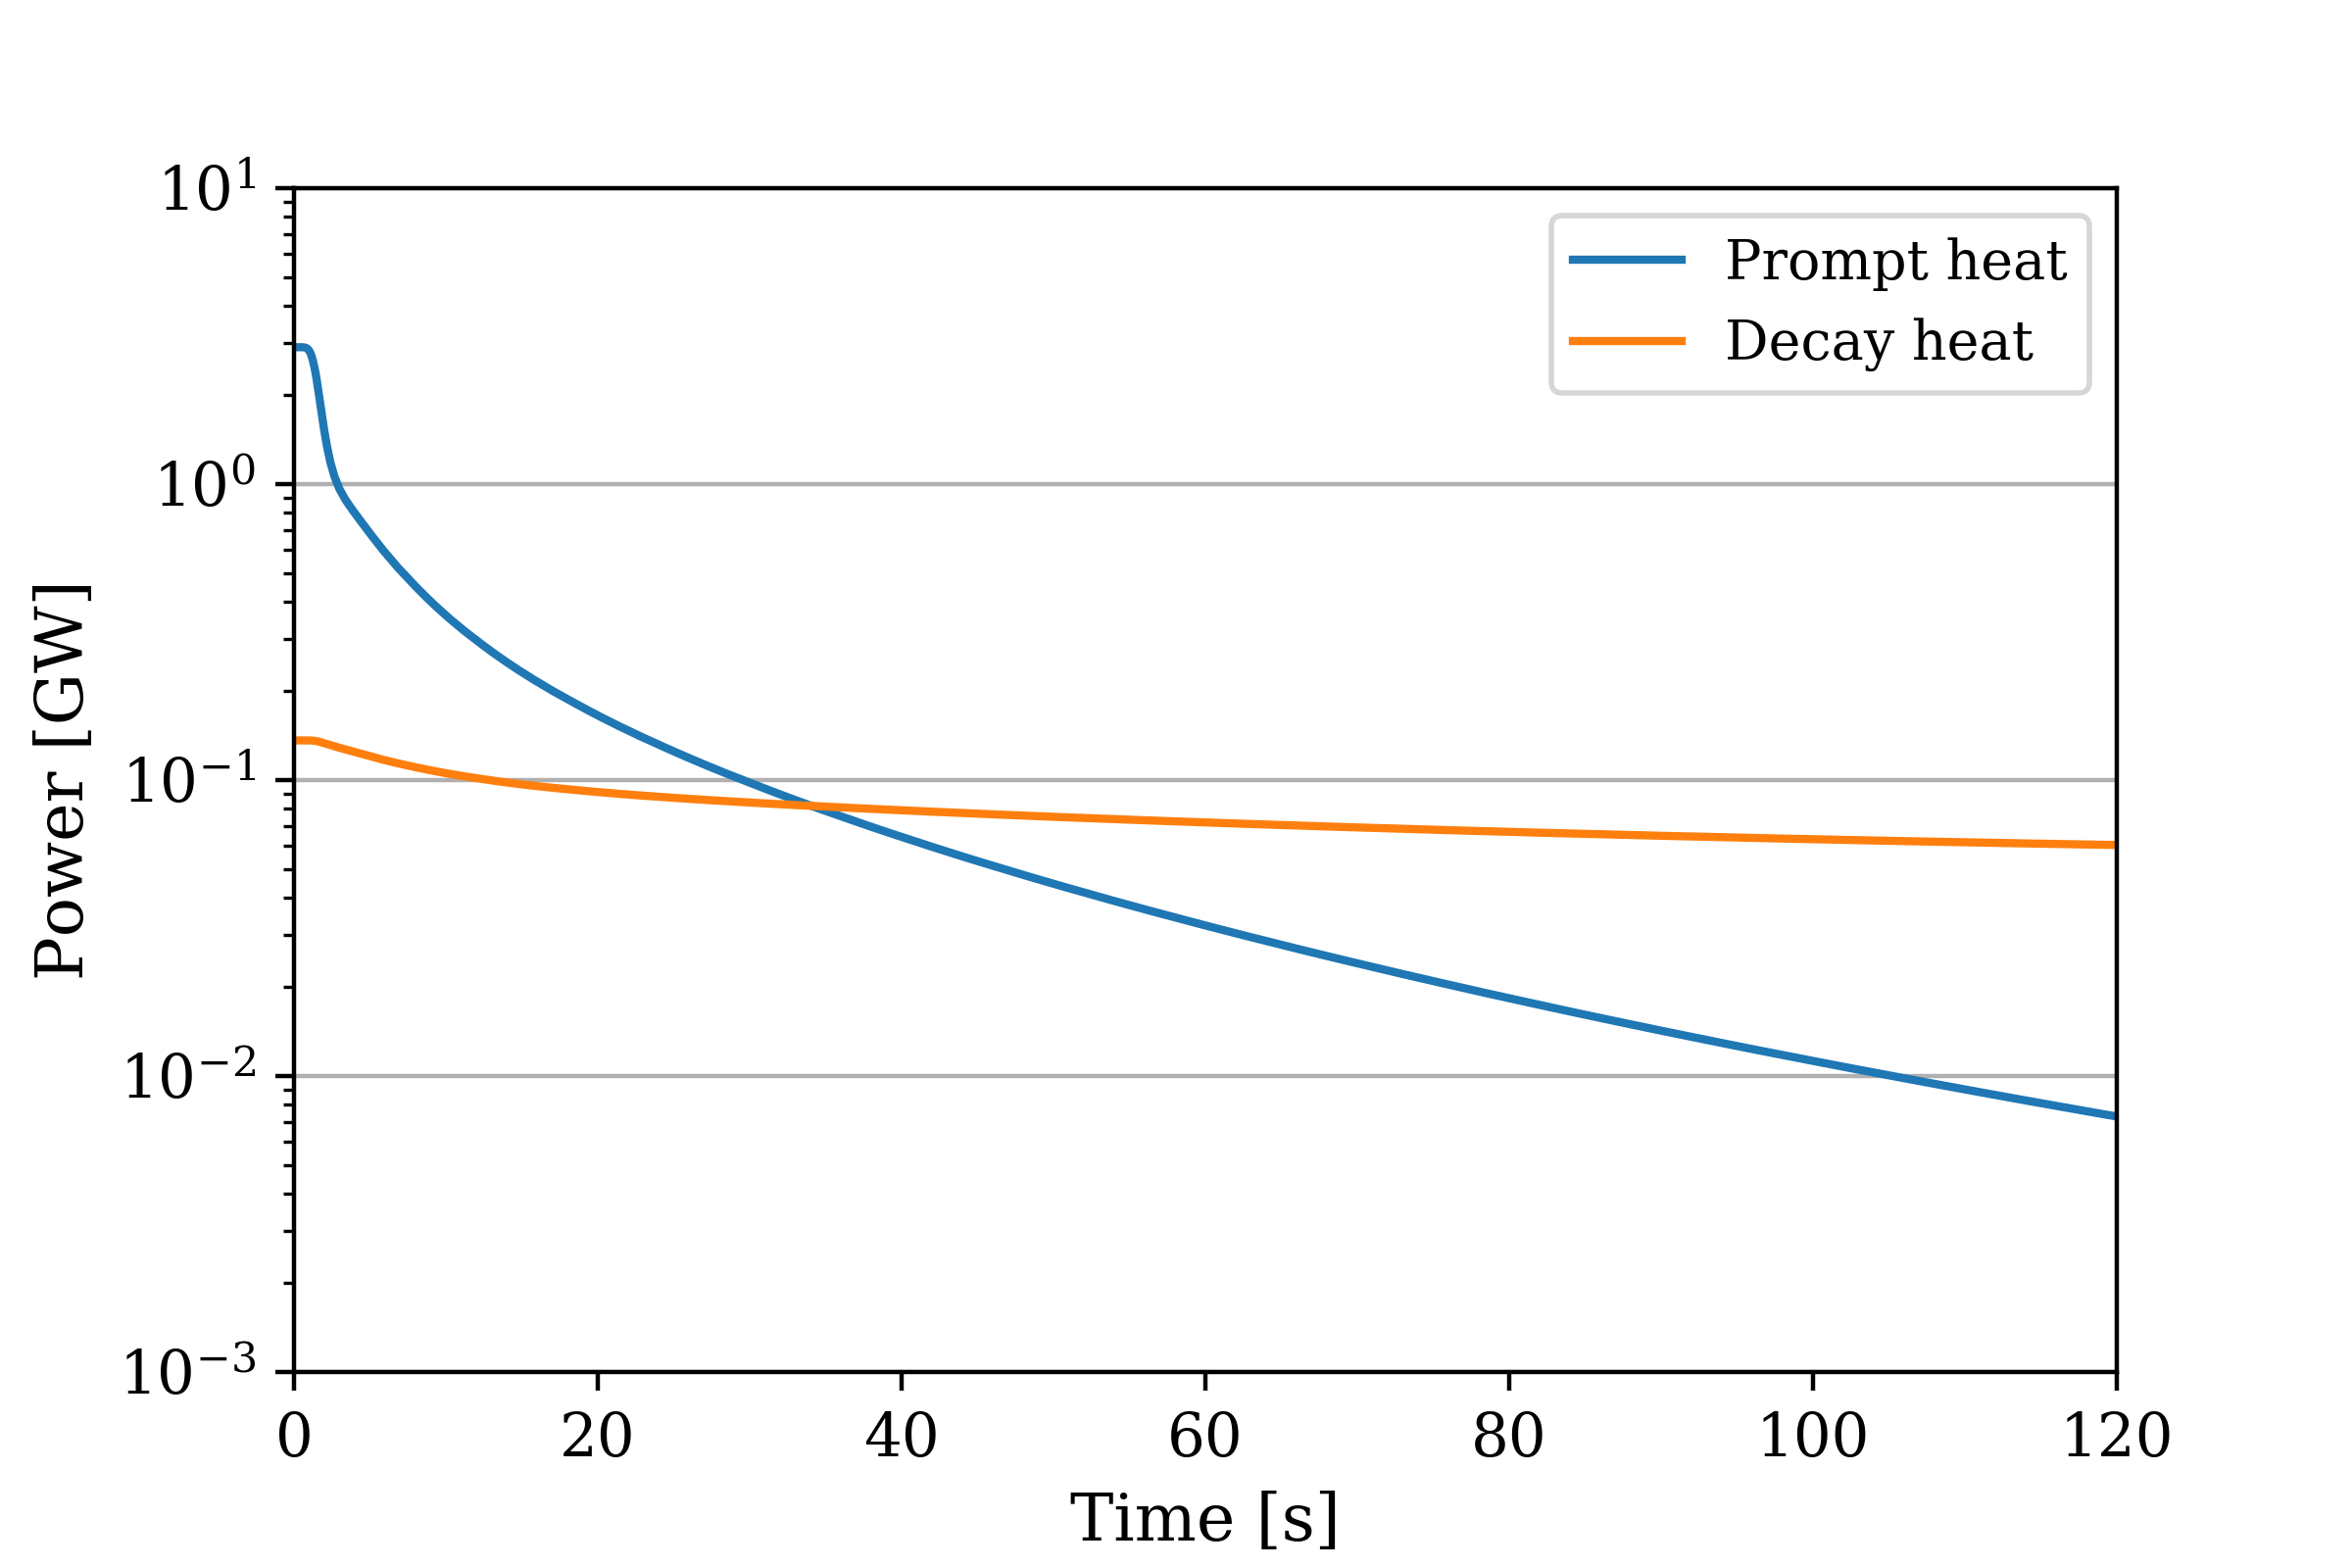
\includegraphics[width=\columnwidth]{moltres-decay-power}
	    \caption{Power output during
    an unprotected loss of heat sink transient in the Moltres model with
    decay heat.}
	    \label{fig:moltresdecaypower}
	\end{minipage}
	\hfill
	\begin{minipage}[t]{0.485\columnwidth}
	    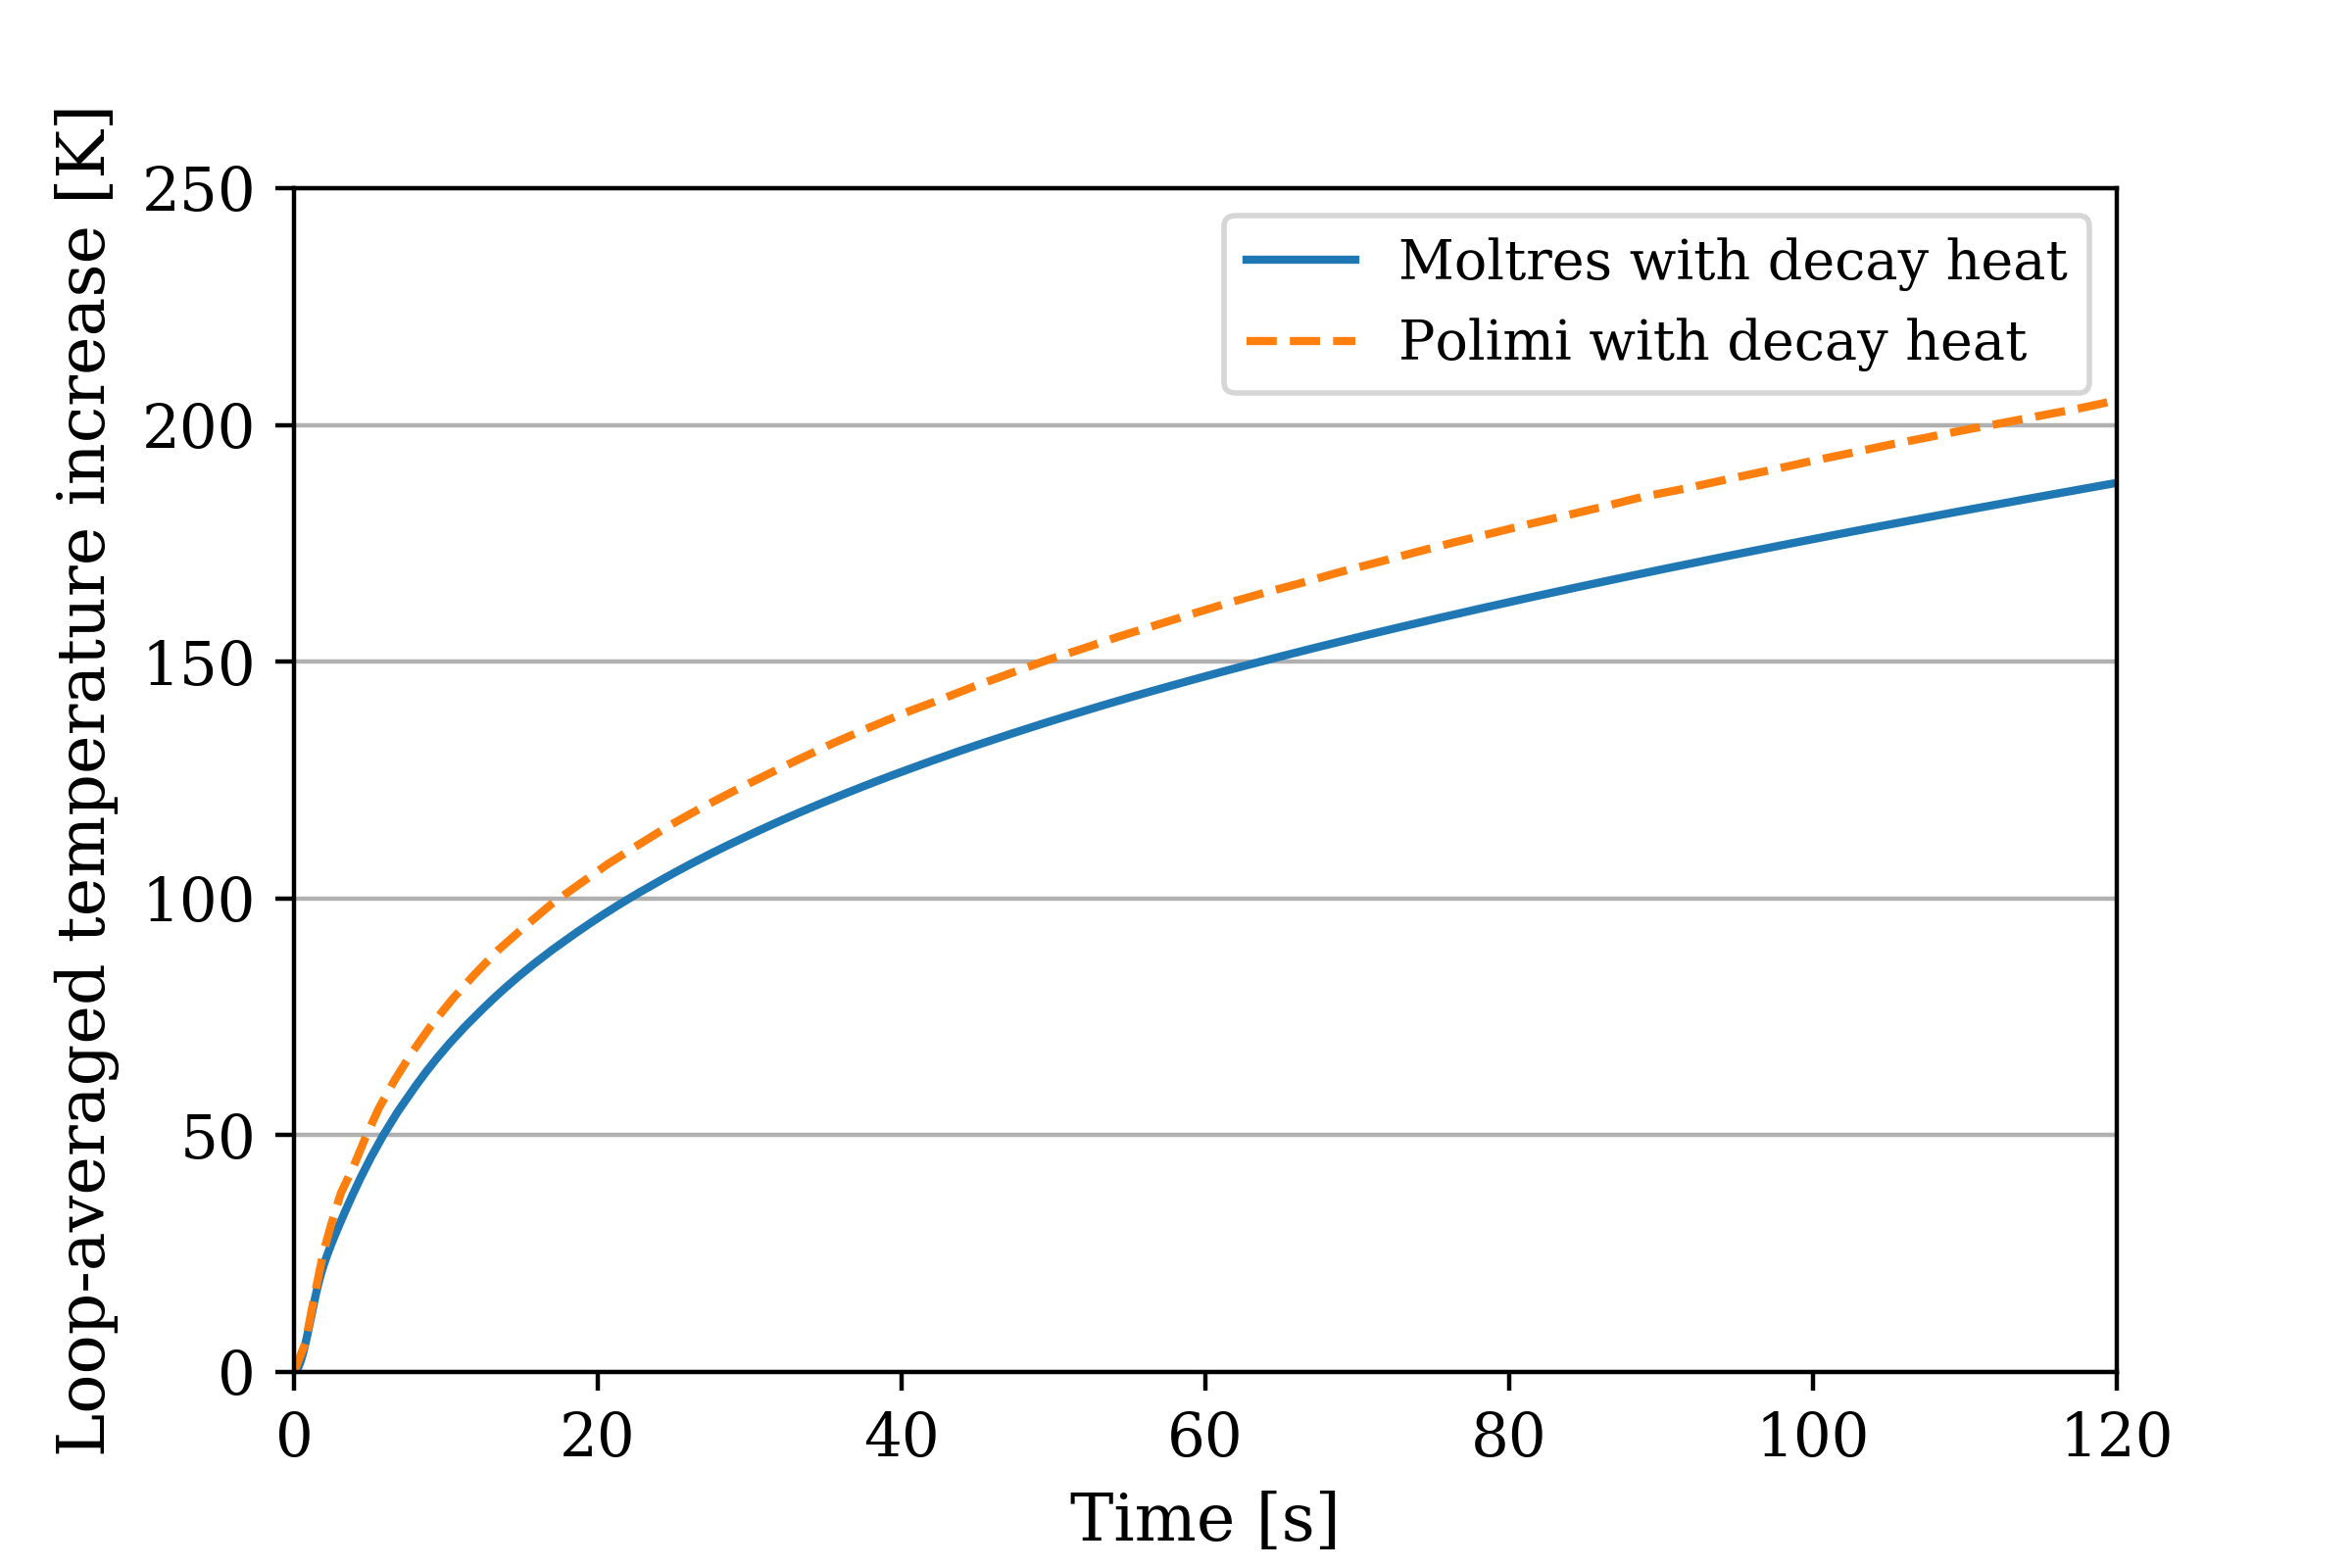
\includegraphics[width=\columnwidth]{decay-temp}
	    \caption{Loop-averaged temperature increase during
    an unprotected loss of heat sink transient in the Moltres and PoliMi
    models \cite{fiorina_modelling_2014} with decay heat.}
	    \label{fig:polimidecaytemp}
	\end{minipage}
\end{figure}

On the other hand, for the pump-initiated accident scenarios, significant
changes in the flow affected the validity of the uniform turbulent viscosity
assumption. These transients required ad hoc adjustments to the uniform
turbulent viscosity assumption as a function of volumetric flow to reproduce
the trends observed in the PoliMi and TU Delft models. Furthermore, unlike the
other two models, the Moltres model did not apply the Boussinesq approximation
for buoyancy-driven flow. The Moltres model could replicate expected trends in
the pump overspeed scenario (Figure \ref{fig:poshort}), but performed
poorly in the loss of flow scenario (Figure \ref{fig:lof}). In the latter
scenario, buoyancy effects become significant as the model loses forced flow.

\begin{figure}[htb!]
    \centering
    \begin{subfigure}[t]{.485\textwidth}
        \centering
        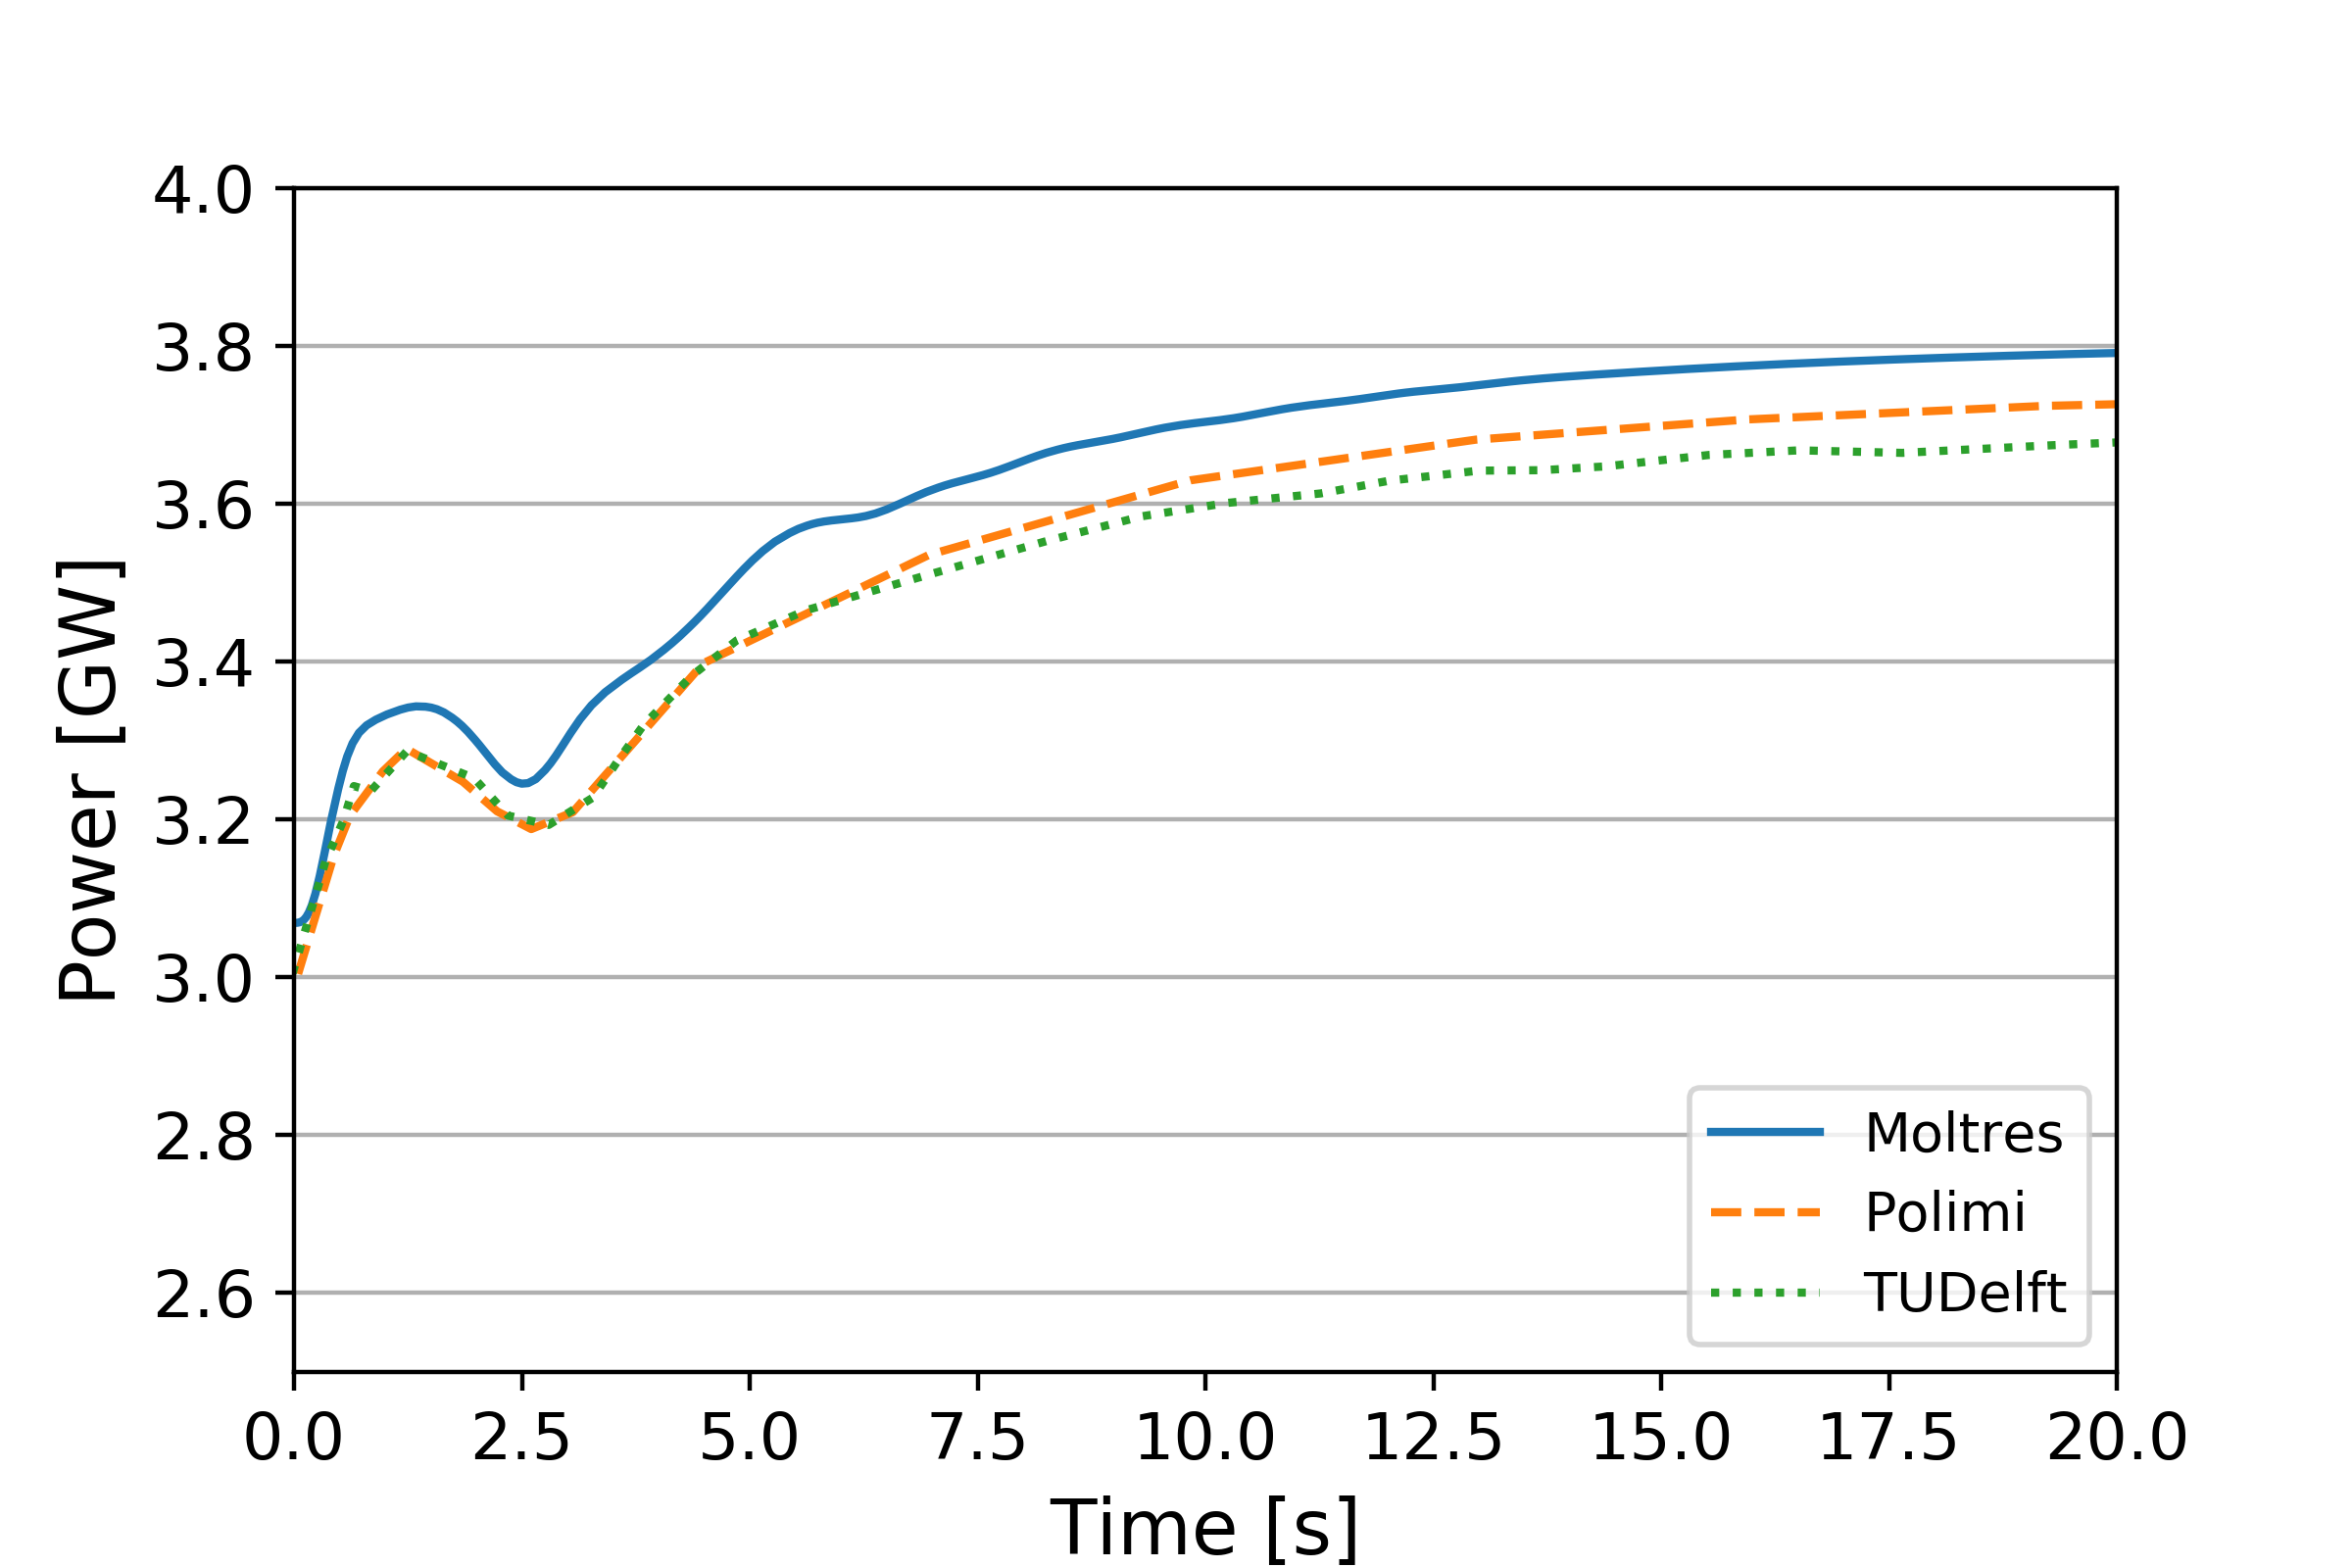
\includegraphics[width=\textwidth]{po-heat-short}
    \end{subfigure}
    \hfill
    \begin{subfigure}[t]{.485\textwidth}
        \centering
        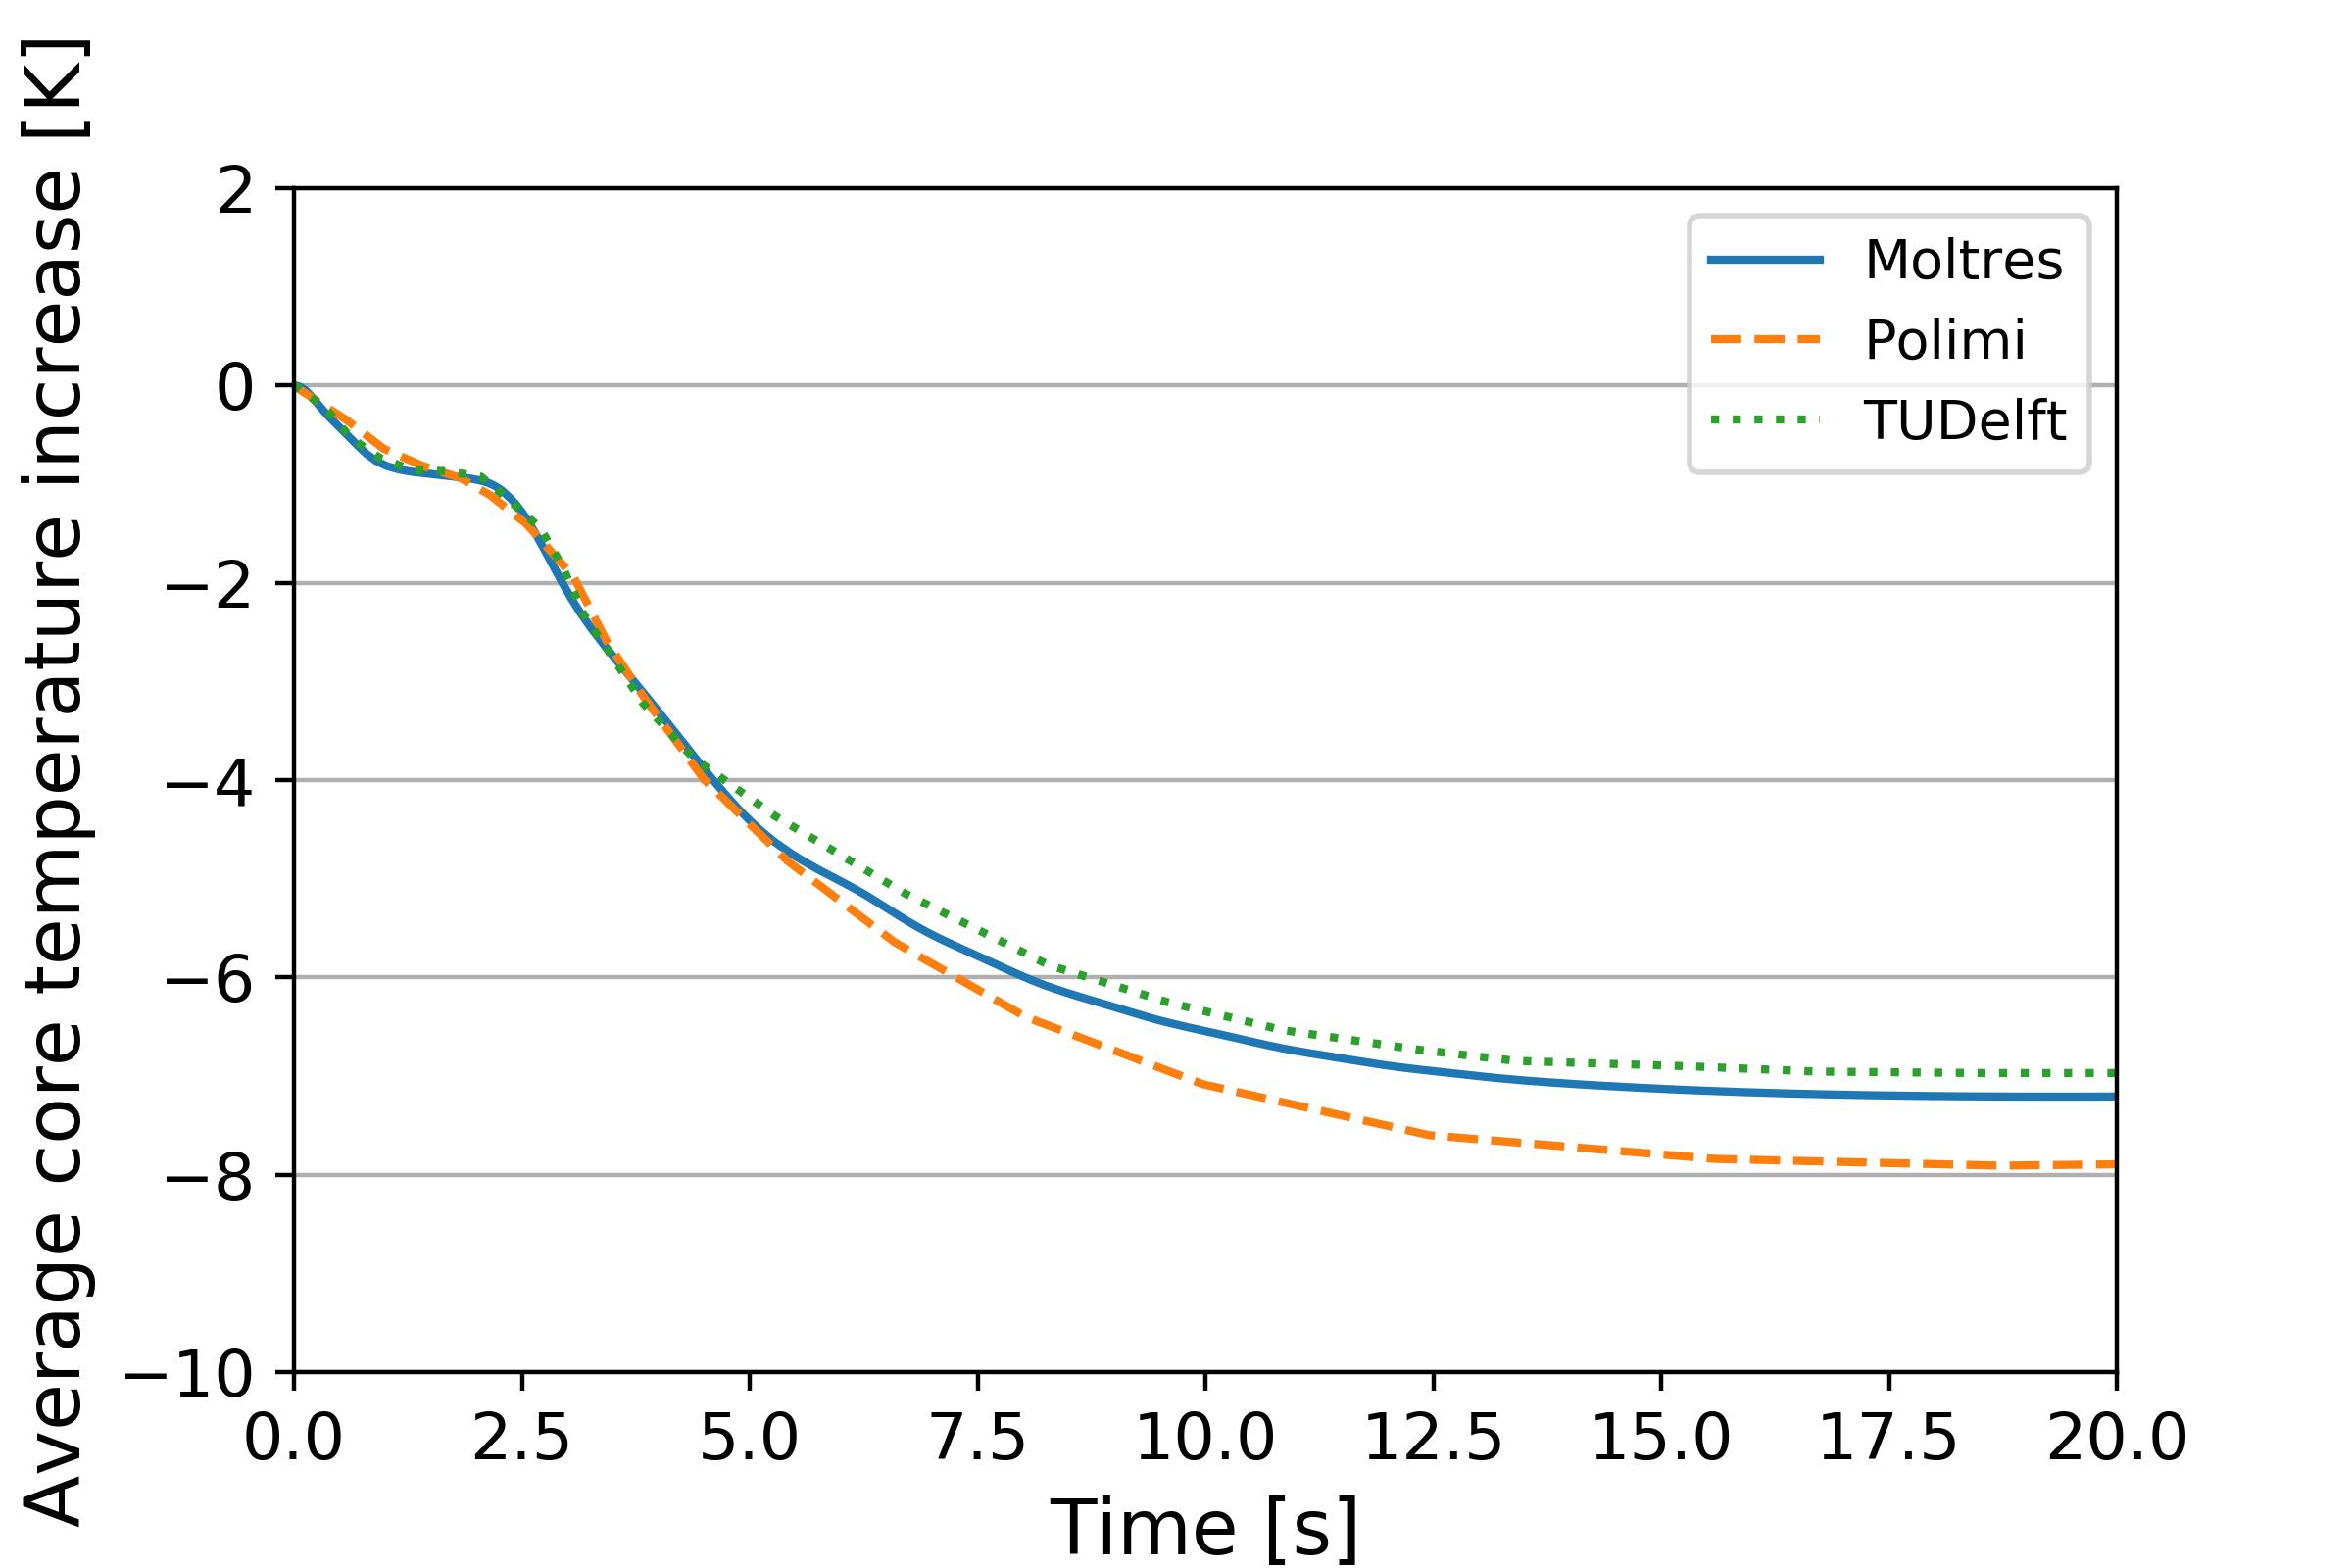
\includegraphics[width=\textwidth]{po-temp-short}
    \end{subfigure}
    \caption{Average core temperature increase during
    an unprotected pump overspeed transient in the Moltres, PoliMi, and
    TU Delft models \cite{fiorina_modelling_2014}.}
    \label{fig:poshort}
\end{figure}

\begin{figure}[htb!]
    \centering
    \begin{subfigure}[t]{.485\textwidth}
        \centering
        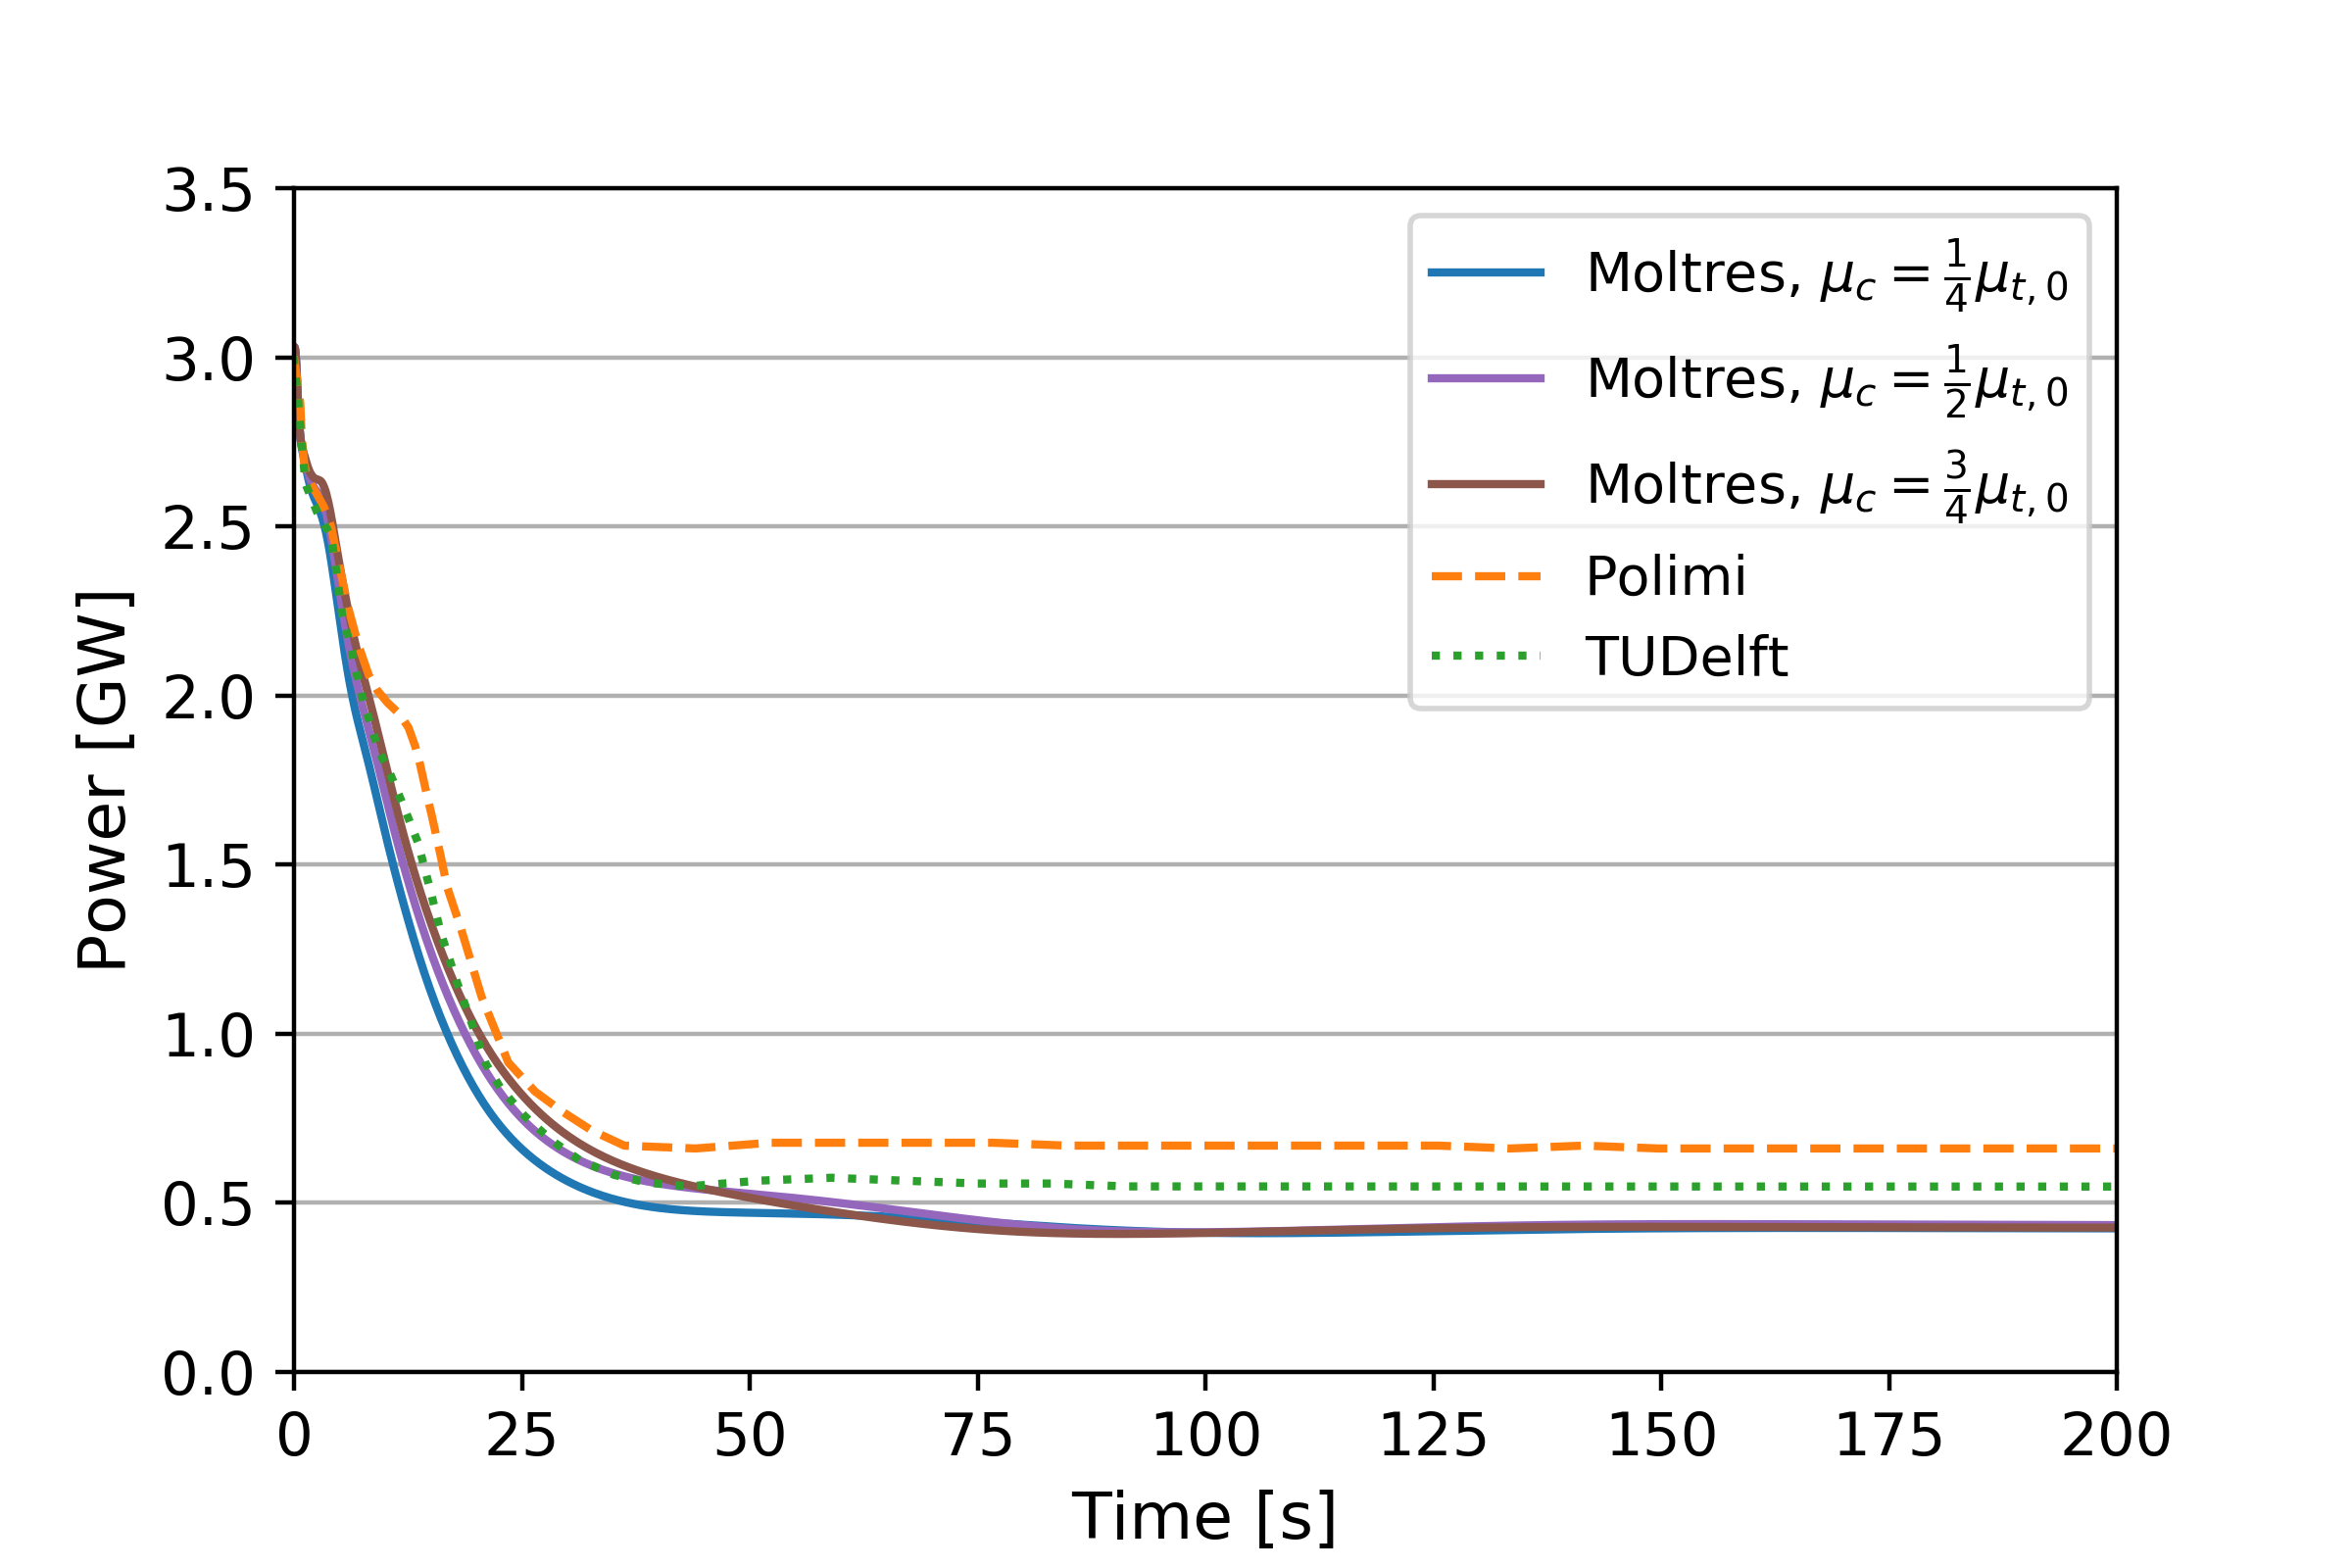
\includegraphics[width=\textwidth]{lof-heat}
    \end{subfigure}
    \hfill
    \begin{subfigure}[t]{.485\textwidth}
        \centering
        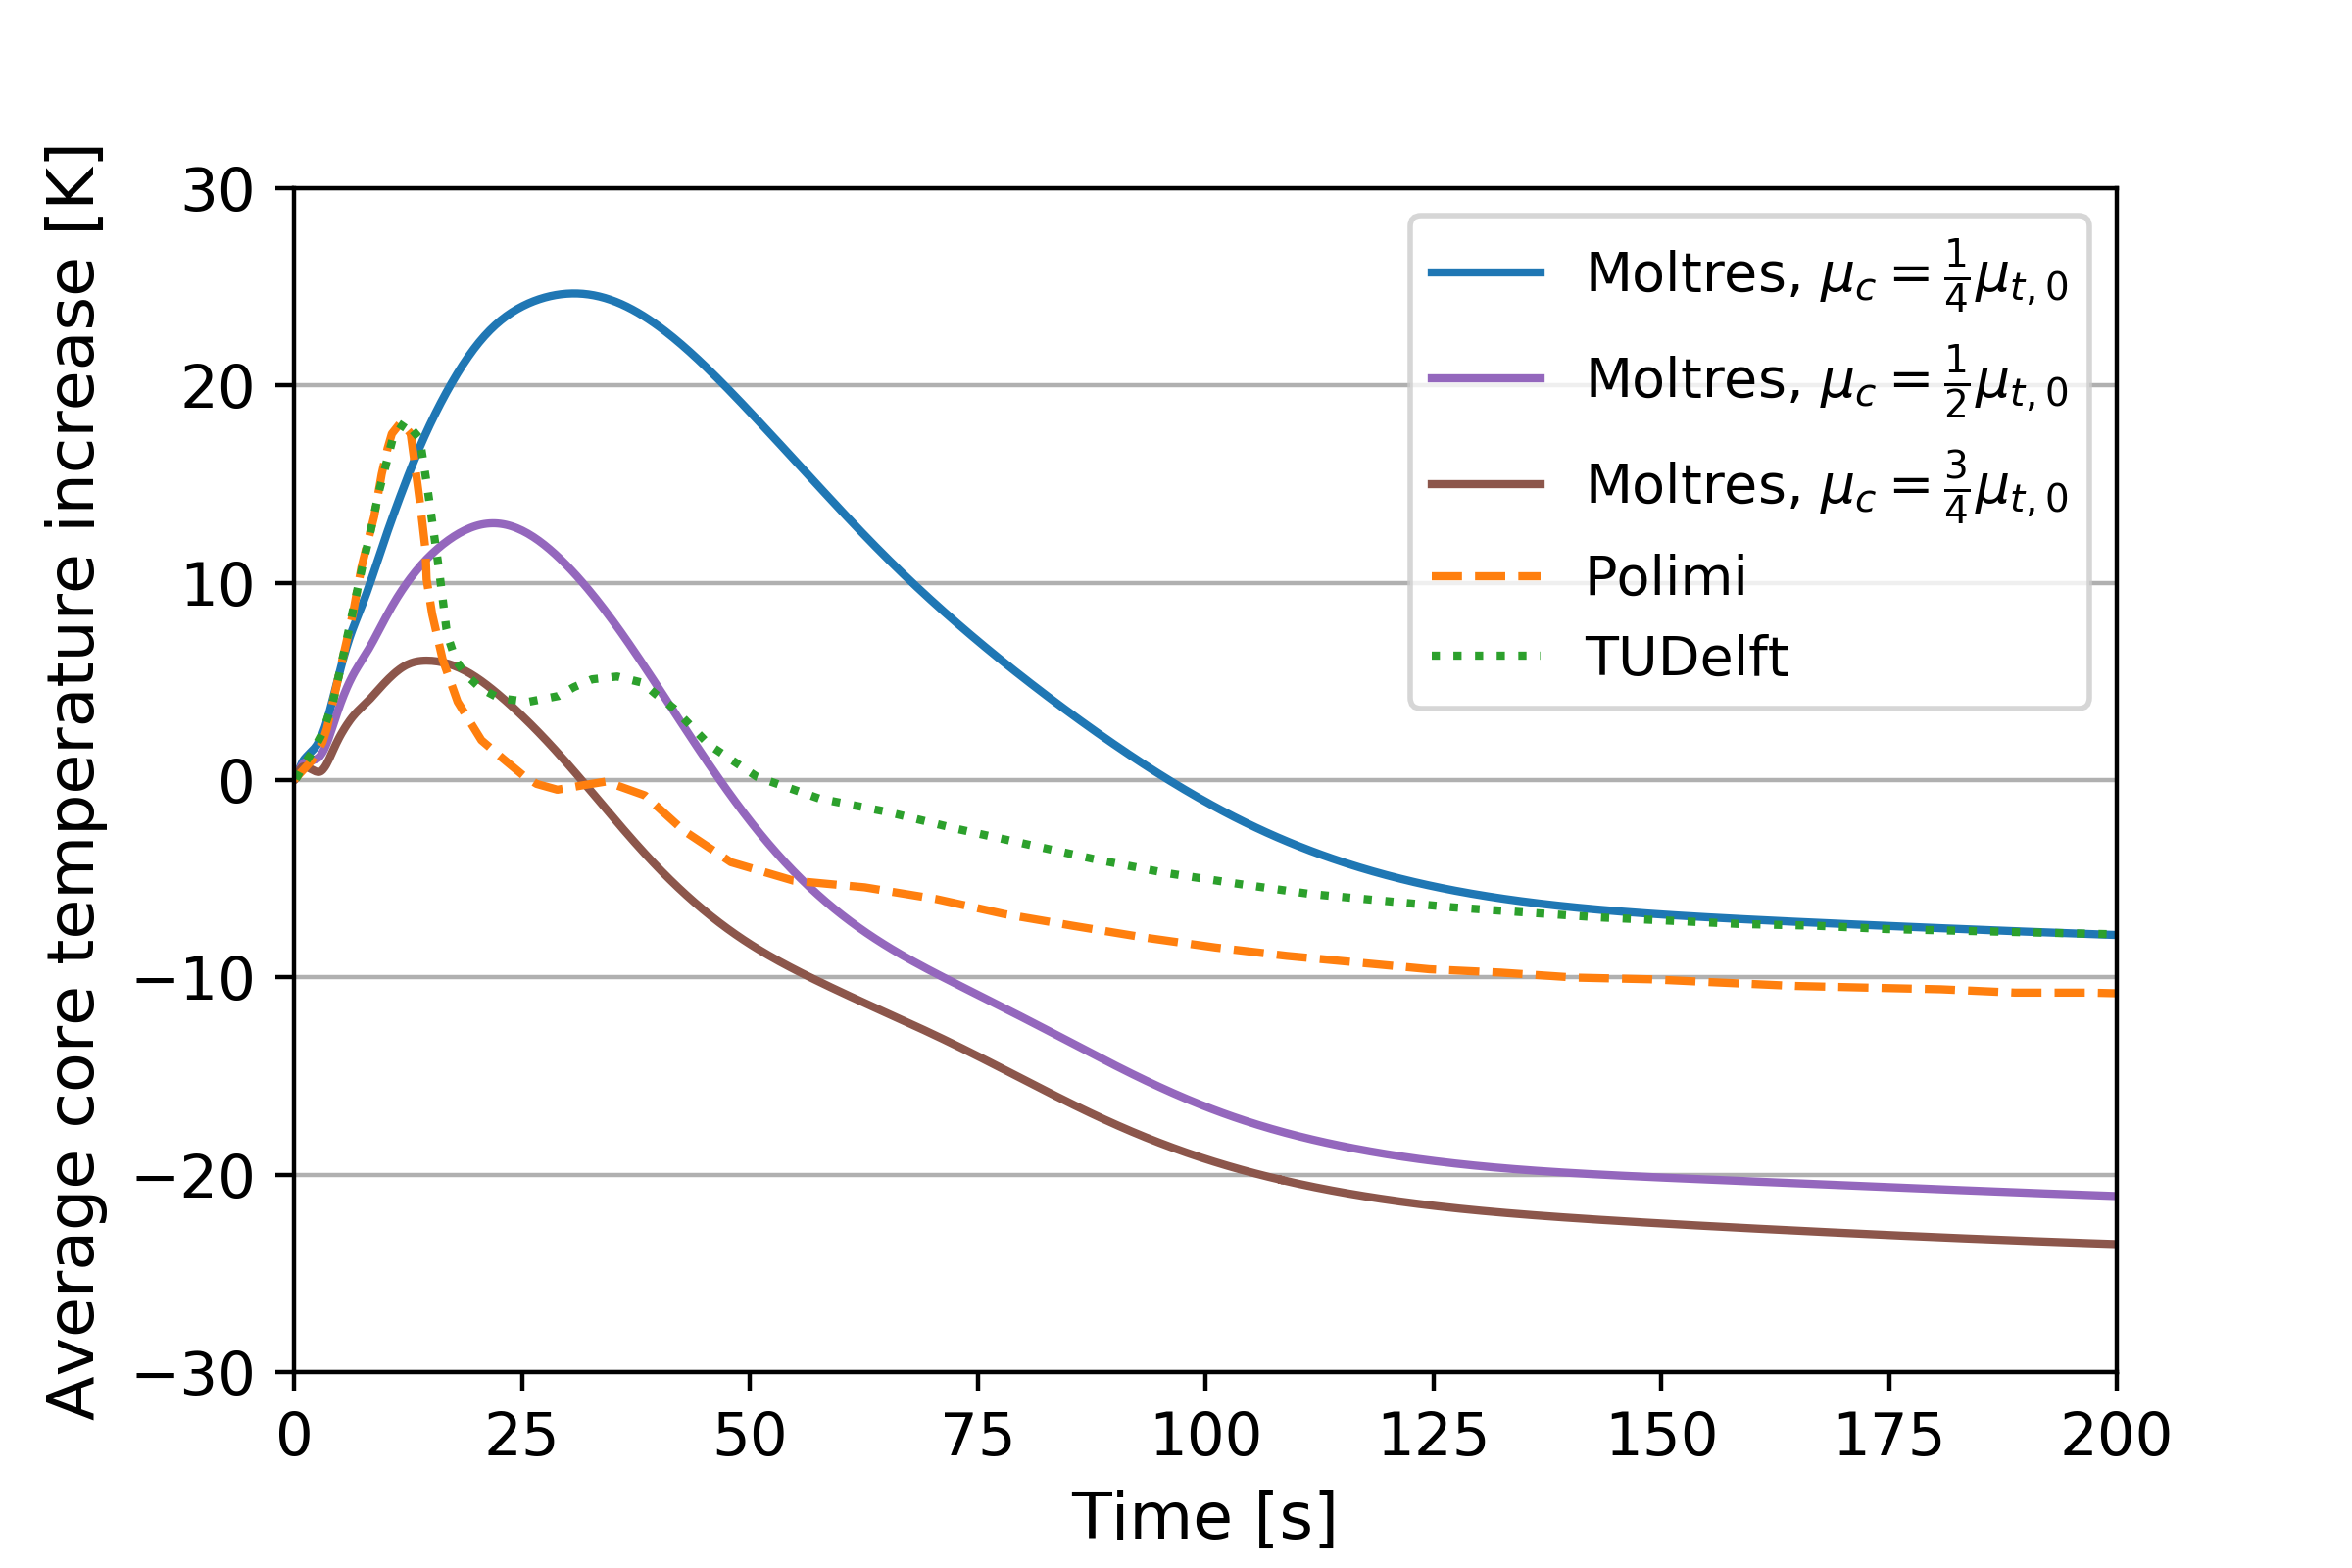
\includegraphics[width=\textwidth]{lof-temp}
    \end{subfigure}
    \caption{Power output and average core temperature increase during
    an unprotected loss of flow transient in the Moltres, PoliMi, and
    TU Delft models \cite{fiorina_modelling_2014}.}
    \label{fig:lof}
\end{figure}

\paragraph{Critical Assessment} \label{sec:msfr-critique}

Given the inherent and unique characteristics of \glspl{MSR}, the new
capabilities introduced in this work---coupling to incompressible Navier-Stokes
equations, precursor loop system, and decay heat model---are essential for
accurate \gls{MSR} modeling and simulation. This work demonstrated these
capabilities through steady-state and transient studies of a 2-D axisymmetric
\gls{MSFR} model similar to models by Fiorina et al.
\cite{fiorina_modelling_2014} and Aufiero et al.
\cite{aufiero_development_2014}. The Moltres model showed good agreement with
the other models in
most steady-state and transient cases with respect to the neutron flux, reactor
power, temperature, and velocity distributions. Most crucially, the
incompressible flow model reproduced characteristic regions of recirculating
flow and near-stagnant flow observed in the PoliMi and TU Delft \gls{MSFR}
models, which led to the formation of temperature hotspots and precursor
accumulation in the core.

However, significant discrepancies observed during pump-initiated transient
scenarios highlight the need for a proper turbulence model to capture
turbulent flow effects in some \gls{MSR} designs. Unlike the \gls{MSRE}, the
\gls{MSFR} experiences highly turbulent flow, whose Reynolds number is on the
order of $10^6$ under normal operating conditions. This level of turbulent flow
produces eddies of a wide range of length scales, and the computational demands
of the fine mesh and time resolution render it numerically unsolvable with
today's computational resources. Turbulence models allow for cheaper turbulence
simulations on coarser meshes by approximating the turbulent effects through
statistical analysis. Fiorina et al. \cite{fiorina_modelling_2014} employed the
$k$-$\epsilon$ turbulence model in their PoliMi and TU Delft models. Moltres
will benefit from coupling to similar intermediate-fidelity turbulence models
for turbulence simulations at reasonable computational costs.

While the Moltres model demonstrated good agreement with published data in the
steady-state, reactivity, and loss of heat sink scenarios, this work does not
thoroughly verify Moltres' capabilities for \gls{MSR} modeling.
The \gls{MSFR} simulations involve various physics models which combine to form
a complex multiphysics model. Therefore, it is difficult to pinpoint sources of
discrepancy with a high degree of certainty. Differences in the modeling
approaches also introduce discrepancies that cannot be reliably identified.
Moltres will benefit from code-to-code verification of
individual components responsible for modeling various physics present in
\glspl{MSR} and Moltres' multiphysics coupling approach.

\section{CNRS Benchmark}

As identified in Section \ref{sec:msfr-critique},
Moltres will benefit from further \gls{VV} of its
\gls{MSR} modeling capabilities. This chapter presents verification
results from Moltres for problems within the CNRS Benchmark
\cite{tiberga_results_2020}---a numerical benchmark specifically designed to
assess \gls{MSR} simulation tools on coupled multiphysics simulations of
fast-spectrum \glspl{MSR}. The benchmark consists of several steps in which
steady-state and transient simulations are prescribed. The benchmark starts with simple
single-physics cases and incrementally introduces various types of
multiphysics coupling until full coupling is simulated in the final steps. This
gradual approach helps participants identify sources of discrepancies
that can arise from differences in modeling assumptions or
cross-section libraries, or actual errors in the software. I adapted the
contents of this chapter from my journal article titled
``\textit{Verification of Moltres for Multiphysics Simulations of Fast-Spectrum
Molten Salt Reactors}'' and published in the Annals of Nuclear Energy journal
\cite{park_verification_2022}.

\subsection{Description of the CNRS Benchmark} \label{sec:benchmark}

The CNRS Benchmark \cite{tiberga_results_2020} is a numerical
benchmark for multiphysics software dedicated to modeling \glspl{MSR}. It
consists of three phases and eight steps in total. Each
step is a well-defined subproblem for systematically assessing the
capabilities of \gls{MSR} software and pinpointing sources of discrepancies
between software. Phase 0 consists of three single-physics problems in fluid
dynamics, neutronics, and temperature. Phase 1 consists
of four coupled steady-state problems. Lastly, Phase 2 consists of one
coupled, time-dependent problem.

\begin{figure}[htb!]
	\centering
	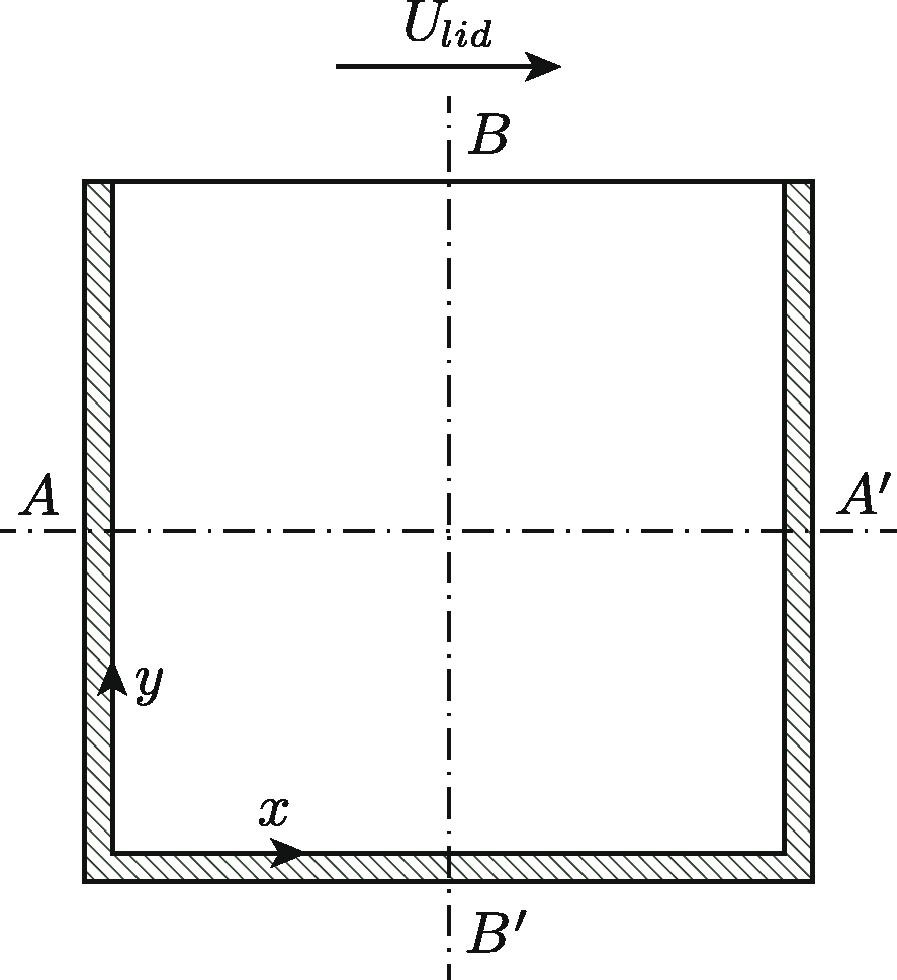
\includegraphics[width=.6\columnwidth]{cnrs-geometry}
	\caption{2m$\times$2m 2D domain of the CNRS Benchmark. $U_{lid}$
	represents the velocity along the top boundary. For comparison, various quantities are
	measured along the centerlines AA' and BB'. From Tiberga et
	al. \cite{tiberga_results_2020}.}
	\label{fig:cnrs-geometry}
\end{figure}

As shown in Figure \ref{fig:cnrs-geometry}, the domain geometry is a
2m$\times$2m square cavity filled with LiF-BeF$_2$-UF$_4$ molten salt at an
initial temperature of 900K \cite{tiberga_results_2020}.
Standard vacuum boundary conditions apply for neutron flux along all
boundaries whereby outgoing neutrons are considered lost, while homogeneous
boundary conditions apply for delayed neutron precursors. No-slip boundary
conditions apply for velocity variables in the cavity, except along the top
boundary for Steps 0.1, 0.3, 1.1, 1.2, and 1.4, which impose forced flow in the
form of lid-driven
cavity flow. For the temperature variable, all boundaries are insulated, and we
simulate salt cooling with the following volumetric heat sink equation:
%
\begin{align}
    q'''(\vec{r}) &= \gamma \left(900 - T(\vec{r})\right) \label{eq:cnrs-heat}
    \shortintertext{where}
    q''' &= \mbox{volumetric heat sink [W$\cdot$m$^{-3}$],}
    \nonumber \\
    \gamma &= \mbox{heat transfer coefficient [W$\cdot$m$^{-3}\cdot$K$^{-1}$],}
    \nonumber \\
    T(\vec{r}) &= \mbox{temperature at point $\vec{r}$ [K].} \nonumber
\end{align}

Tiberga et al. \cite{tiberga_results_2020} used Serpent 2
\cite{leppanen_serpent_2014} with the JEFF-3.1 library
\cite{koning_jeff-31_2006} to generate multigroup neutronics data for the
LiF-BeF$_2$-UF$_4$ salt in the domain at 900K, which they condensed into six
energy groups and eight precursor groups. We direct readers to their paper for
the group constant data \cite{tiberga_results_2020}. In addition, the
benchmark prescribes the following equations to govern the temperature
dependence in the cross sections and the neutron diffusion coefficients:
%
\begin{align}
    \Sigma_i (T) &= \Sigma_i(T_{ref})
    \frac{\rho_{fuel}(T)}{\rho_{fuel}(T_{ref})}
    \shortintertext{and}
    D (T) &= D(T_{ref})
    \frac{\rho_{fuel}(T_{ref})}{\rho_{fuel}(T)}
    \shortintertext{where}
    \Sigma_i &= \mbox{relevant macroscopic cross section [cm${-1}$],}
    \nonumber \\
    D &= \mbox{neutron diffusion coefficient [cm$^2\cdot$s$^{-1}$],}   
    \nonumber \\
    \rho_{fuel} &= \mbox{density of the fuel salt [kg$\cdot$m$^{-3}$],}
    \nonumber \\
    T_{ref} &= \mbox{reference temperature} = 900\mbox{ K}. \nonumber
\end{align}

The benchmark also prescribes incompressible Navier-Stokes flow with the
Boussinesq approximation for evaluating the salt flow in the
domain but does not restrict the type of neutronics model.
Table \ref{table:benchmark} lists the relevant input parameters and observables.

\begin{table*}[tp!]
	\caption{Input parameters and observables of each benchmark step.}
	\centering
	\footnotesize
    \begin{tabular}{p{.05\textwidth} p{.1\textwidth} p{.3\textwidth} p{.45\textwidth}}
		\toprule
        \textbf{Step} & \textbf{Name} & \textbf{Input parameters} & \textbf{Observables} \\
		\midrule
        0.1 & Velocity field &
		\begin{itemize}[nosep,noitemsep,left=0pt,
		                before={\begin{minipage}[t]{\hsize}},
                        after ={\end{minipage}}]
		    \item $U_{lid} = 0.5$ m$\cdot$s$^{-1}$
		\end{itemize}\vspace*{-\baselineskip}\mbox{} &
		\begin{itemize}[nosep,noitemsep,left=0pt,
		                before={\begin{minipage}[t]{\hsize}},
                        after ={\end{minipage}}]
		    \item Velocity components $(u_x,u_y)$ along AA' and BB'
		\end{itemize}\vspace*{-\baselineskip}\mbox{} \\
        \midrule
        0.2 & Neutronics &
        \begin{itemize}[nosep,noitemsep,left=0pt,
		                before={\begin{minipage}[t]{\hsize}},
                        after ={\end{minipage}}]
		    \item $U_{lid} = 0$ m$\cdot$s$^{-1}$
		    \item $T = 900$ K
		    \item $P = 1$ GW
		\end{itemize} &
		\begin{itemize}[nosep,noitemsep,left=0pt,
		                before={\begin{minipage}[t]{\hsize}},
                        after ={\end{minipage}}]
		    \item Fission rate density $\sum^6_g \Sigma_{f,g} \phi_g(\vec{r})$ along AA'
            \item Reactivity $\rho$
		\end{itemize}\vspace*{-\baselineskip}\mbox{} \\
        \midrule
        0.3 & Temperature &
        \begin{itemize}[nosep,noitemsep,left=0pt,
		                before={\begin{minipage}[t]{\hsize}},
                        after ={\end{minipage}}]
		    \item Fixed flow field from Step 0.1 for
		    $U_{lid} = 0.5$ m$\cdot$s$^{-1}$
		    \item Fixed heat source distribution
		    $\sum^6_{g} \epsilon_g \Sigma_{f,g} \phi_g(\vec{r})$ from Step 0.2
		    \item $\gamma = 10^6$ W$\cdot$m$^{-3}\cdot$K$^{-1}$
		\end{itemize} &
		\begin{itemize}[nosep,noitemsep,left=0pt,
		                before={\begin{minipage}[t]{\hsize}},
                        after ={\end{minipage}}]
		    \item Temperature $T$ along AA' and BB'
		\end{itemize}\vspace*{-\baselineskip}\mbox{} \\
        \midrule
        1.1 & Circulating fuel &
        \begin{itemize}[nosep,noitemsep,left=0pt,
		                before={\begin{minipage}[t]{\hsize}},
                        after ={\end{minipage}}]
		    \item Fixed flow field from Step 0.1 for
		    $U_{lid} = 0.5$ m$\cdot$s$^{-1}$
		    \item $T = 900$ K
		    \item $P = 1$ GW
		\end{itemize} &
		\begin{itemize}[nosep,noitemsep,left=0pt,
		                before={\begin{minipage}[t]{\hsize}},
                        after ={\end{minipage}}]
		    \item Delayed neutron source $\sum^8_i \lambda_i C_i$ along AA' and BB'
		    \item Reactivity change between Step 1.1 and Step 0.2,
		    $\Delta \rho = \rho - \rho_{s_{0.2}}$
		\end{itemize}\vspace*{-\baselineskip}\mbox{} \\
        \midrule
        1.2 & Power coupling &
        \begin{itemize}[nosep,noitemsep,left=0pt,
		                before={\begin{minipage}[t]{\hsize}},
                        after ={\end{minipage}}]
		    \item Fixed flow field from Step 0.1 for
		    $U_{lid} = 0.5$ m$\cdot$s$^{-1}$
		    \item $P = 1$ GW
		    \item $\gamma = 10^6$ W$\cdot$m$^{-3}\cdot$K$^{-1}$
		\end{itemize}\vspace*{-\baselineskip}\mbox{} &
		\begin{itemize}[nosep,noitemsep,left=0pt,
		                before={\begin{minipage}[t]{\hsize}},
                        after ={\end{minipage}}]
		    \item Temperature $T$ along AA' and BB'
            \item Reactivity change between Step 1.2 and Step 1.1,
            $\Delta\rho = \rho - \rho_{s_{1.1}}$
            \item Change in fission rate density
            $\sum^6_g \Sigma_{f,g} \phi_g(\vec{r}) -
            \left[\sum^6_g \Sigma_{f,g} \phi_g(\vec{r})\right]_{s_{0.2}}$
		\end{itemize} \\
        \midrule
        1.3 & Buoyancy &
        \begin{itemize}[nosep,noitemsep,left=0pt,
		                before={\begin{minipage}[t]{\hsize}},
                        after ={\end{minipage}}]
		    \item $P = 1$ GW
		    \item $U_{lid} = 0$ m$\cdot$s$^{-1}$
		    \item $\gamma = 10^6$ W$\cdot$m$^{-3}\cdot$K$^{-1}$
		\end{itemize}\vspace*{-\baselineskip}\mbox{} &
		\begin{itemize}[nosep,noitemsep,left=0pt,
		                before={\begin{minipage}[t]{\hsize}},
                        after ={\end{minipage}}]
		    \item Velocity components $(u_x, u_y)$ along AA' and BB'
            \item Temperature $T$ along AA' and BB'
            \item Delayed neutron source $\sum^8_i \lambda_i C_i$ along AA' and BB'
            \item Reactivity change from Step 0.2
        $\Delta\rho = \rho - \rho_{s_{0.2}}$
		\end{itemize} \\
        \midrule
        1.4 & Full coupling &
        \begin{itemize}[nosep,noitemsep,left=0pt,
		                before={\begin{minipage}[t]{\hsize}},
                        after ={\end{minipage}}]
		    \item $\gamma = 10^6$ W$\cdot$m$^{-3}\cdot$K$^{-1}$
		    \item $P$ variable in the range $[0,1]$ GW with a step of 0.2 GW
		    \item $U_{lid}$ variable in the range $[0,0.5]$ m$\cdot$s$^{-1}$
		    with a step of 0.1 m$\cdot$s$^{-1}$
		\end{itemize} &
		\begin{itemize}[nosep,noitemsep,left=0pt,
		                before={\begin{minipage}[t]{\hsize}},
                        after ={\end{minipage}}]
		    \item Reactivity change between Step 1.4 and Step 0.2,
		    $\Delta\rho = \rho - \rho_{s_{0.2}}$, for all permutations of $P$
		    and $U_{lid}$ values
		\end{itemize}\vspace*{-\baselineskip}\mbox{} \\
        \midrule
        2.1 & Forced convection transient &
        \begin{itemize}[nosep,noitemsep,left=0pt,
		                before={\begin{minipage}[t]{\hsize}},
                        after ={\end{minipage}}]
		    \item $\gamma = 10^6$ W$\cdot$m$^{-3}\cdot$K$^{-1}$
            \item Steady-state solution from Step 1.4 for $U_{lid} = 0.5$
        m$\cdot$s$^{-1}$ and $P = 1.0$ GW
		\end{itemize} &
		\begin{itemize}[nosep,noitemsep,left=0pt,
		                before={\begin{minipage}[t]{\hsize}},
                        after ={\end{minipage}}]
		    \item Power gain and shift as a function of the perturbation frequency
		\end{itemize}\vspace*{-\baselineskip}\mbox{} \\
		\bottomrule
	\end{tabular}
	\label{table:benchmark}
\end{table*}

Step 2.1 studies the transient response of the fully coupled nonlinear system.
Linear perturbation analyses are performed by introducing periodic
perturbations to the heat transfer coefficient $\gamma$ and studying the gain
and phase shift of the response in the total power $P$. For the initial
conditions, the steady-state solution from Step 1.4 with
$U_{lid} = 0.5$ m$\cdot$s$^{-1}$ and $P = 1$ GW is used. This initial
configuration is made exactly critical by scaling the neutron source terms,
from fission and \gls{DNP} decay, by the inverse of the criticality eigenvalue
solution from Step 1.4.

$\gamma$ is uniformly perturbed according to small-amplitude sine waves given
as:
%
\begin{align}
    \gamma =& \gamma_0 \left[ 1 + 0.1\sin\left(2 \pi f \right) \right]
    \shortintertext{where}
    \gamma_0 =& 10^6 \mbox{ W$\cdot$m$^{-3}\cdot$K$^{-1}$}, \nonumber \\
    f \in& \left\lbrace 0.0125, 0.025, 0.05, 0.1, 0.2, 0.4, 0.8 \right\rbrace 
    \mbox{ Hz.} \nonumber
\end{align}

The benchmark defines power gain as:
%
\begin{align}
    \mbox{Power gain} =& \frac{\left(P_{max} - P_{avg}\right)/P_{avg}}{
    \left(\gamma_{max} - \gamma_{avg}\right)/\gamma_{avg}}
\end{align}
%
The subscripts denote the maximum and time-averaged values of $P$ and $\gamma$.

\FloatBarrier

\subsection{Modeling Approach with Moltres} \label{sec:model}

This section describes the specific modeling approach for
simulating the CNRS Benchmark cases in Moltres.

For this work\footnote{The input files for
all benchmark
cases are available on the Moltres GitHub repository at 
\url{https://github.com/arfc/moltres/tree/devel/problems/2021-cnrs-benchmark}.
}, I ran the benchmark cases on a uniformly-spaced mesh
of 200$\times$200 elements. Thus, the dimensions of each mesh element are
0.01m$\times$0.01m. I adopted the group constant data
provided by Tiberga et al. \cite{tiberga_results_2020}. Next, I
discretized most variables, i.e., neutron fluxes, velocity
components, pressure, and temperature, using continuous, first-order, Lagrange
shape functions. The only exception is the precursor concentration variables,
which I discretized using zeroth-order monomial shape functions and solved
using a \gls{DFEM}. I interpolated the resulting discontinuous,
cell-centered precursor values to obtain the nodal values for results
analysis.

The
\texttt{Navier-Stokes} and \texttt{Heat} \texttt{Conduction} modules from
\gls{MOOSE} provide some of the capabilities for
modeling incompressible flow and heat transfer. In particular, I stabilized
the incompressible flow and temperature governing equations using the
\gls{SUPG} stabilization method implemented in \gls{MOOSE}
\cite{peterson_overview_2018}. Without \gls{SUPG} stabilization, I
observed spurious numerical oscillations in the velocity and temperature near
the top boundary due to the singularity on the top left corner where different
velocity boundary conditions meet. I also applied the \gls{PSPG} stabilization
scheme \cite{hughes_new_1986} from the Navier-Stokes module
\cite{peterson_overview_2018},
which enables equal-order discretizations in the velocity and pressure
variables. Equal-order discretizations with \gls{PSPG} are computationally
cheaper and more convenient than implementing higher-order
velocity discretizations for stability without \gls{PSPG}
\cite{chapelle_inf-sup_1993}.

Using the inverse power method solver in \gls{MOOSE}, I ran all eigenvalue calculations in
Steps 0.2, 1.1, 1.2, 1.3, and 1.4. I ran all other steps
using the Preconditioned Newton-Krylov solver
\cite{gaston_physics-based_2015}. The coupled steady-state problems in
Steps 1.2, 1.3, and 1.4 required segregated solvers for the neutronics
and the thermal-hydraulics due to the unique problem setups involving a
criticality search problem for the neutron multiplication factor
and a steady-state problem in thermal-hydraulics simultaneously.

\begin{table}[tb]
    \caption{Timestep sizes used for the time-dependent cases in
    Step 2.1, corresponding to 1/200th of the perturbation period.}
	\centering
	\setlength\tabcolsep{2.5pt}
	\begin{tabular}{l l l l l l l l}
	    \toprule
	    Frequency [Hz] & 0.0125 & 0.025 & 0.05 & 0.1 & 0.2 & 0.4 & 0.8 \\
	    \midrule
	    Timestep size [s] & 0.2 & 0.2 & 0.1 & 0.05 & 0.025 & 0.0125 & 0.00625
	    \\
	    \bottomrule
	\end{tabular}
	\label{table:timestep}
\end{table}

For the time-dependent cases in Step 2.1, I employed full coupling with
a second-order implicit Backward Differential Formula (BDF2) time-stepping
scheme. I set the timestep sizes for each driving frequency in the heat transfer
coefficient to 1/200th of the perturbation period. Table
\ref{table:timestep} shows the timestep sizes. I assumed the
systems reached asymptotic behavior when the magnitudes of neighboring power
peaks differed by less than 0.001\% for at least ten wavelengths. Under this
assumption, the phase shift measurements between adjacent waves always
converged before the magnitude measurements of the power peaks.

Table \ref{table:software} compares the numerical methods, meshing schemes, and
neutronics models of Moltres and the four participating software packages in
the CNRS benchmark paper \cite{tiberga_results_2020}. The $SP_N$ and
$S_N$ neutronics models refer to the simplified $P_N$ spherical harmonics and
$S_N$ discrete ordinates neutron transport models, respectively. Based on the
solvers and methods of solution, Moltres is most similar to the
PHANTOM-$S_N$ + DGFlows \cite{tiberga_discontinuous_2019} multiphysics package
from \gls{TUD} with the $S_2$ neutron transport model. Participants from
\gls{CNRS} and \gls{PSI}
employed non-uniform meshes which were refined near the boundaries. In contrast,
we and the \gls{PoliMi} and \gls{TUD} participants employed uniform meshes.

\FloatBarrier

\begin{landscape}
\begin{table*}[p]
    \caption{List of software packages and their corresponding model
    specifications for the CNRS Benchmark simulations
    \cite{tiberga_results_2020}.}
    \centering
    \begin{tabular}{p{4.2cm} p{7cm} p{3.3cm} p{2cm} p{2.7cm}}
        \toprule
        Software & Institute & Numerical method & Mesh & Neutronics model \\
        \midrule
        OpenFOAM & Centre national de la recherche scientifique (CNRS) & Finite volume & 200$\times$200 \newline Non-uniform & $SP_1$ \& $SP_3$ \\
        OpenFOAM & Politecnico di Milano (PoliMi) & Finite volume & 400$\times$400 \newline Uniform & Neutron diffusion \\
        GeN-Foam & Paul Scherrer Institute (PSI) & Finite volume & 200$\times$200 \newline Non-uniform & Neutron diffusion \\
        PHANTOM-$S_N$+DGFlows & Delft University of Technology (TUD) & Discontinuous finite \newline element & 50$\times$50 \newline Uniform & $S_2$ \& $S_6$ \\
        Moltres (This work) & University of Illinois at Urbana-Champaign (UIUC) & Continuous \& discontinuous finite element & 200$\times$200 \newline Uniform & Neutron diffusion \\
        \bottomrule
    \end{tabular}
    \label{table:software}
\end{table*}
\end{landscape}

\FloatBarrier

\subsection{Results \& Discussion}

In this section, we compare the results from Moltres for each CNRS Benchmark
step to the results in the benchmark paper \cite{tiberga_results_2020}.
The software packages from \gls{CNRS} and \gls{TUD}
each report two sets of results from different angular discretizations
in their neutronics models for Steps 0.2, 1.1, 1.2, 1.3, 1.4, and 2.1. These
sets of results are labeled as CNRS-$SP_1$ and
CNRS-$SP_3$; and TUD-$S_2$ and TUD-$S_6$, respectively. The
authors performed code-to-code verification by sampling observable values at
201 equidistant points along the centerlines AA' and BB' and reporting the
discrepancy $\epsilon_c$ of each observable from each software
(indexed by $c$) for each measured observable $Q_c$ (not to be confused with
fission heat source $Q_f$), relative to the average of
that same observable $Q_{avg}$ from all participating software. Variables
$\epsilon_c$ and $Q_{avg}$ are calculated as:
%
\begin{align}
    \epsilon_c =& \sqrt{\frac{\sum^{N_p}_{i=1}\left[Q_c(\vec{r_i}) - Q_{avg}
    (\vec{r_i})\right]^2}{\sum^{N_p}_{i=1} Q^2_{avg}(\vec{r_i})}}
    \shortintertext{and}
    Q_{avg}(\vec{r_i}) =& \frac{1}{N_c} \sum^{N_c}_{c=1} Q_c(\vec{r_i})
    \shortintertext{where}
    Q_c(\vec{r_i}) =&
    \mbox{ value of observable $Q$ at location $\vec{r_i}$ from software $c$,}
    \nonumber \\
    N_p =& \mbox{ number of sampling points of quantity $Q$} = 201,
    \nonumber \\
    N_c =& \mbox{ number of participating software packages.} \nonumber
\end{align}

The average discrepancy $\epsilon$ across all software is calculated as:
%
\begin{align}
    \epsilon =& \frac{1}{N_c}\sum^{N_c}_{c=1} \epsilon_c
\end{align}

We adopted the averaged values $\epsilon$ and $Q_{avg}$ directly from the
reference work \cite{tiberga_results_2020} without including our results
in the calculations. We note that the benchmark does not provide a reference
solution, and a significantly erroneous value from one of the software packages
could heavily skew the discrepancy values. Nevertheless, the benchmark paper
reports good agreement among their software packages.

For observables measured along the centerlines AA' and BB', Tables
\ref{table:disc0} and \ref{table:disc1} report the discrepancy $\epsilon_c$ of
each observable from Moltres relative to the average of the benchmark
participants $Q_{avg}$ alongside the average discrepancy $\epsilon$ of
the benchmark participants. We also reproduce corresponding plots
in the benchmark paper for every observable along AA' or BB' in Figures
\ref{fig:0.1}, \ref{fig:0.2}, \ref{fig:0.3}, \ref{fig:1.1}, \ref{fig:1.2},
\ref{fig:1.3}, and \ref{fig:2.1} for a qualitative comparison of the results
from Moltres and the benchmark participants. Given the significant overlap in
the plot curves, these figures omit results from CNRS-$SP_1$ and TUD-$S_2$ to
reduce cluttering. The full dataset
of all observable results used in this results analysis is
available at \cite{park_results_2021}. Lastly, Table
\ref{table:rho} reports all reactivity and reactivity changes from
Steps 0.2, 1.1, 1.2, and 1.3.

\begin{figure}[h]
	\centering
    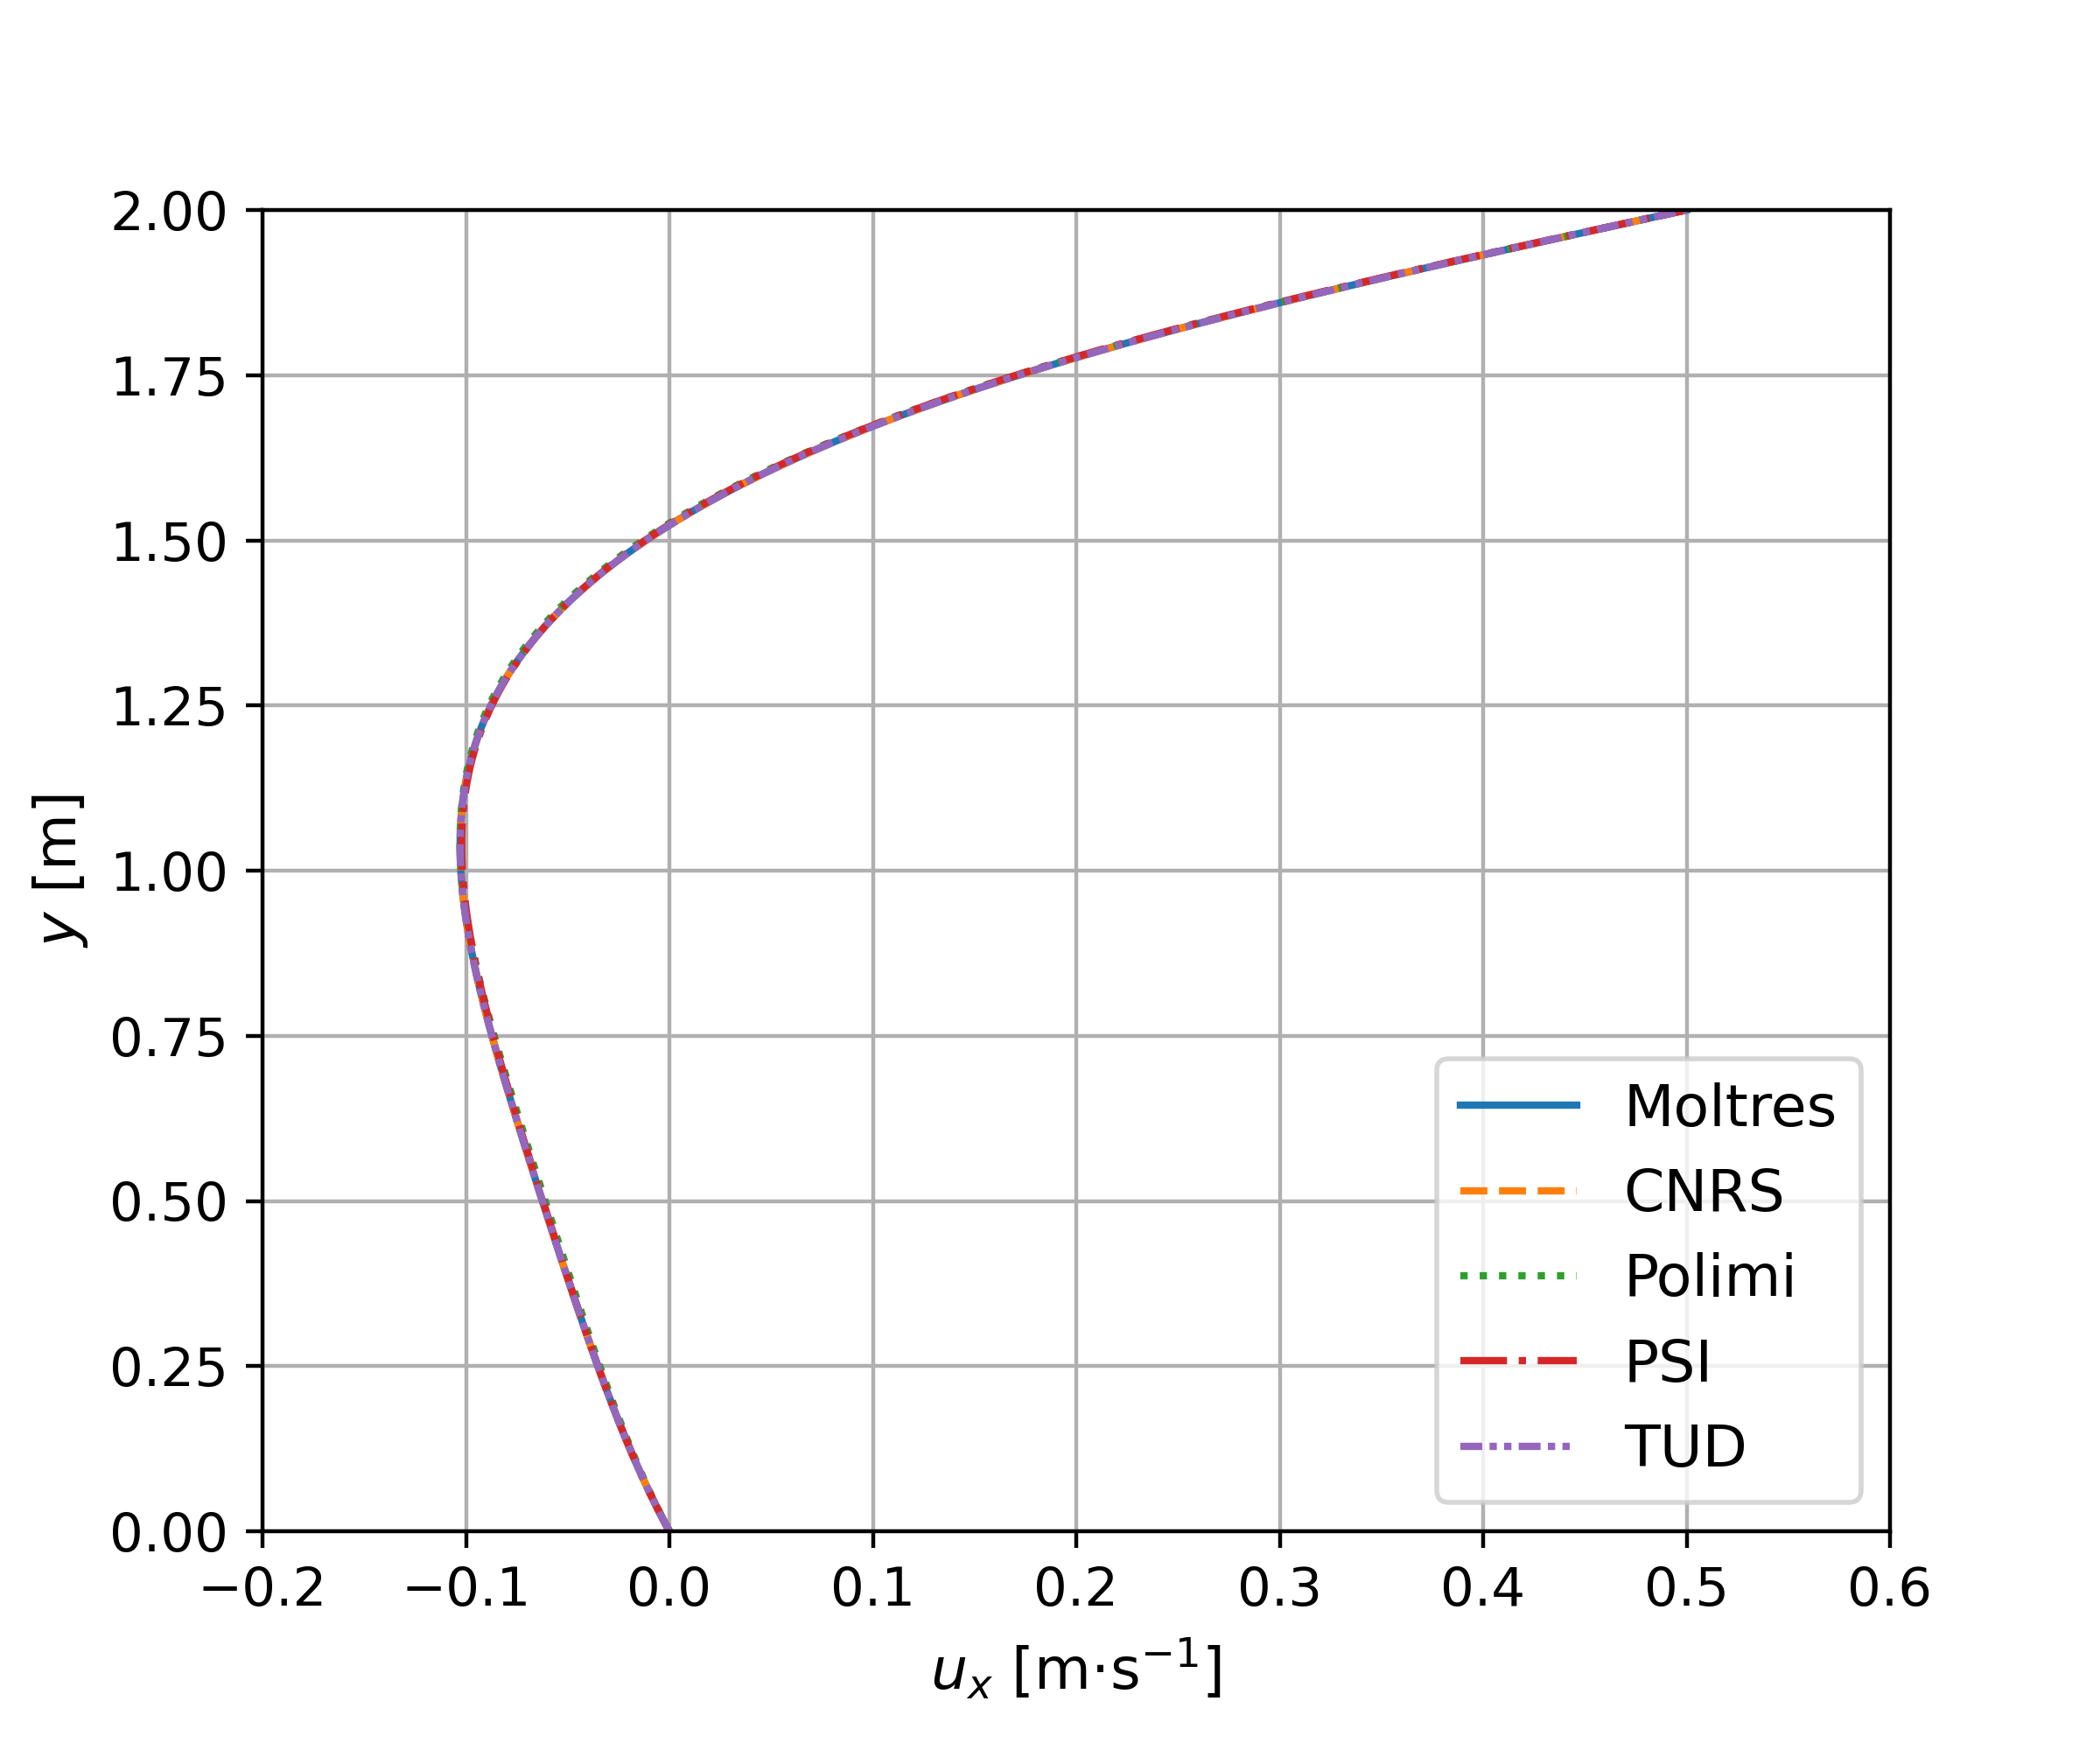
\includegraphics[width=.49\columnwidth]{0-1-vel-plot}
	\caption{Step 0.1 \textemdash\ Horizontal velocity component along BB'.}
	\label{fig:0.1}
\end{figure}
%
\begin{figure}[h]
	\centering
    \begin{subfigure}[b]{.49\textwidth}
      \centering
	  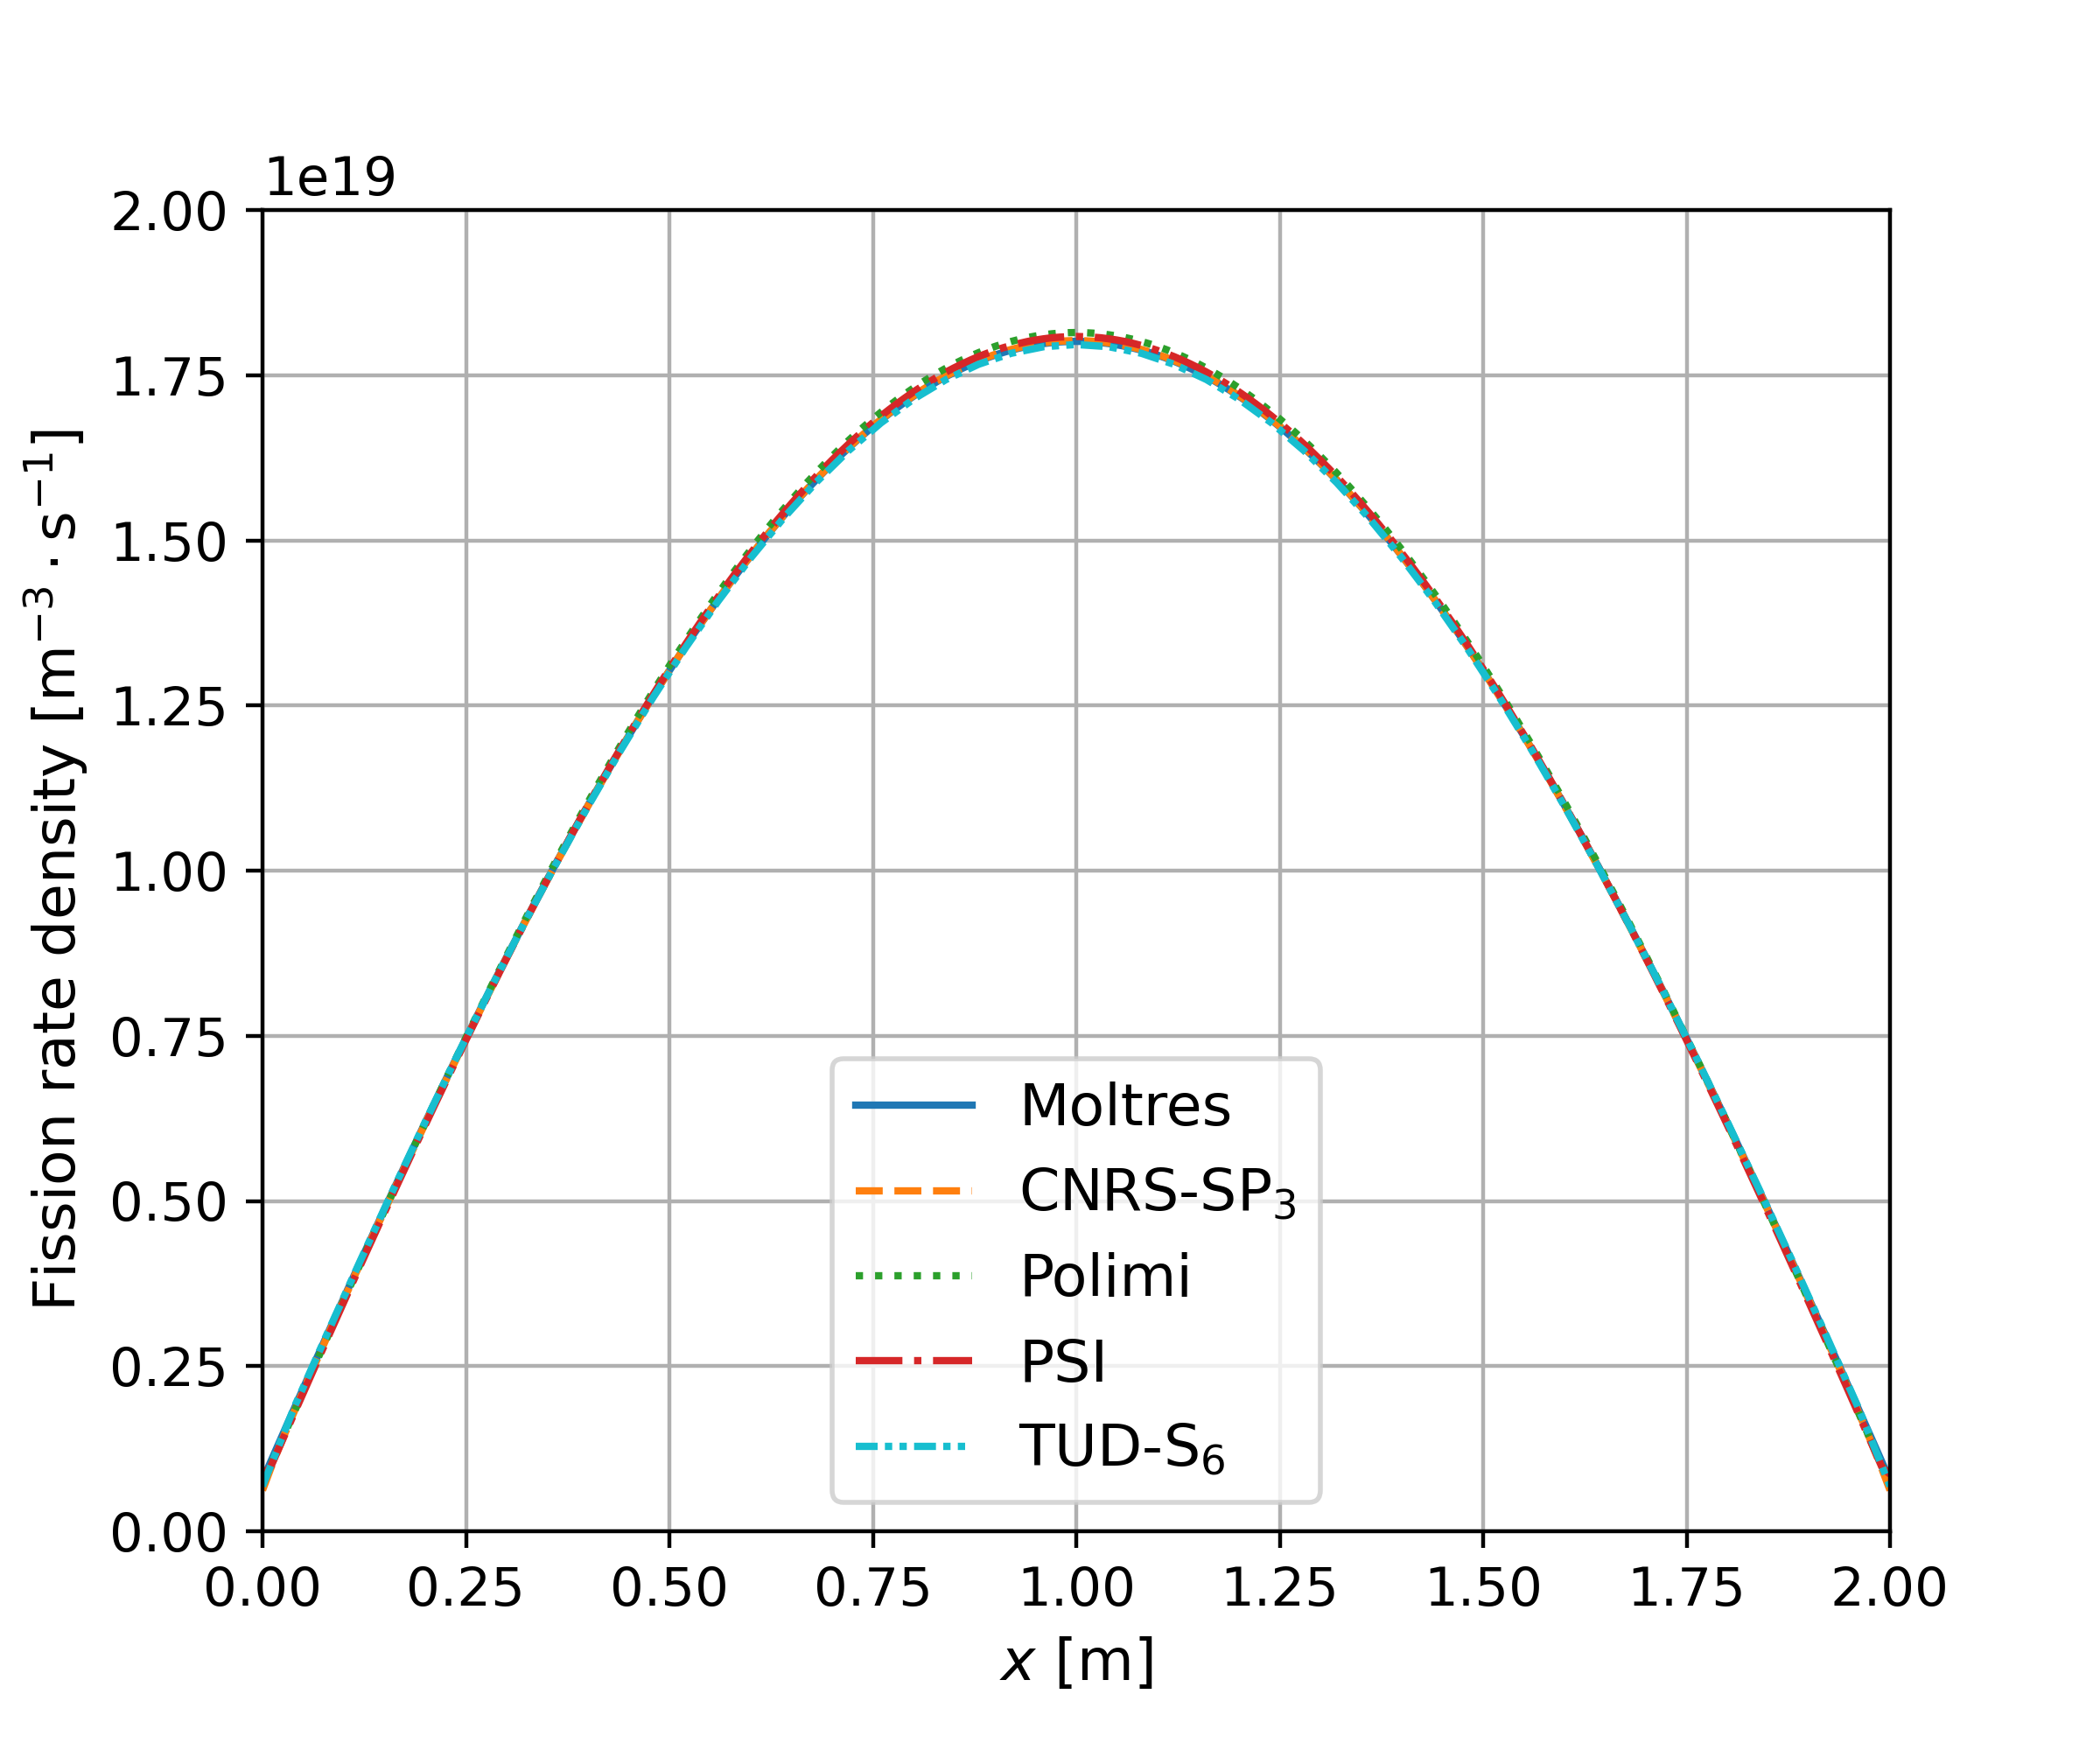
\includegraphics[width=\columnwidth]{0-2-fiss-plot}
	  \caption{Step 0.2 \textemdash\ Fission rate density along AA'.}
	  \label{fig:0.2}
    \end{subfigure}
    \hfill
    \begin{subfigure}[b]{.49\textwidth}
      \centering
	  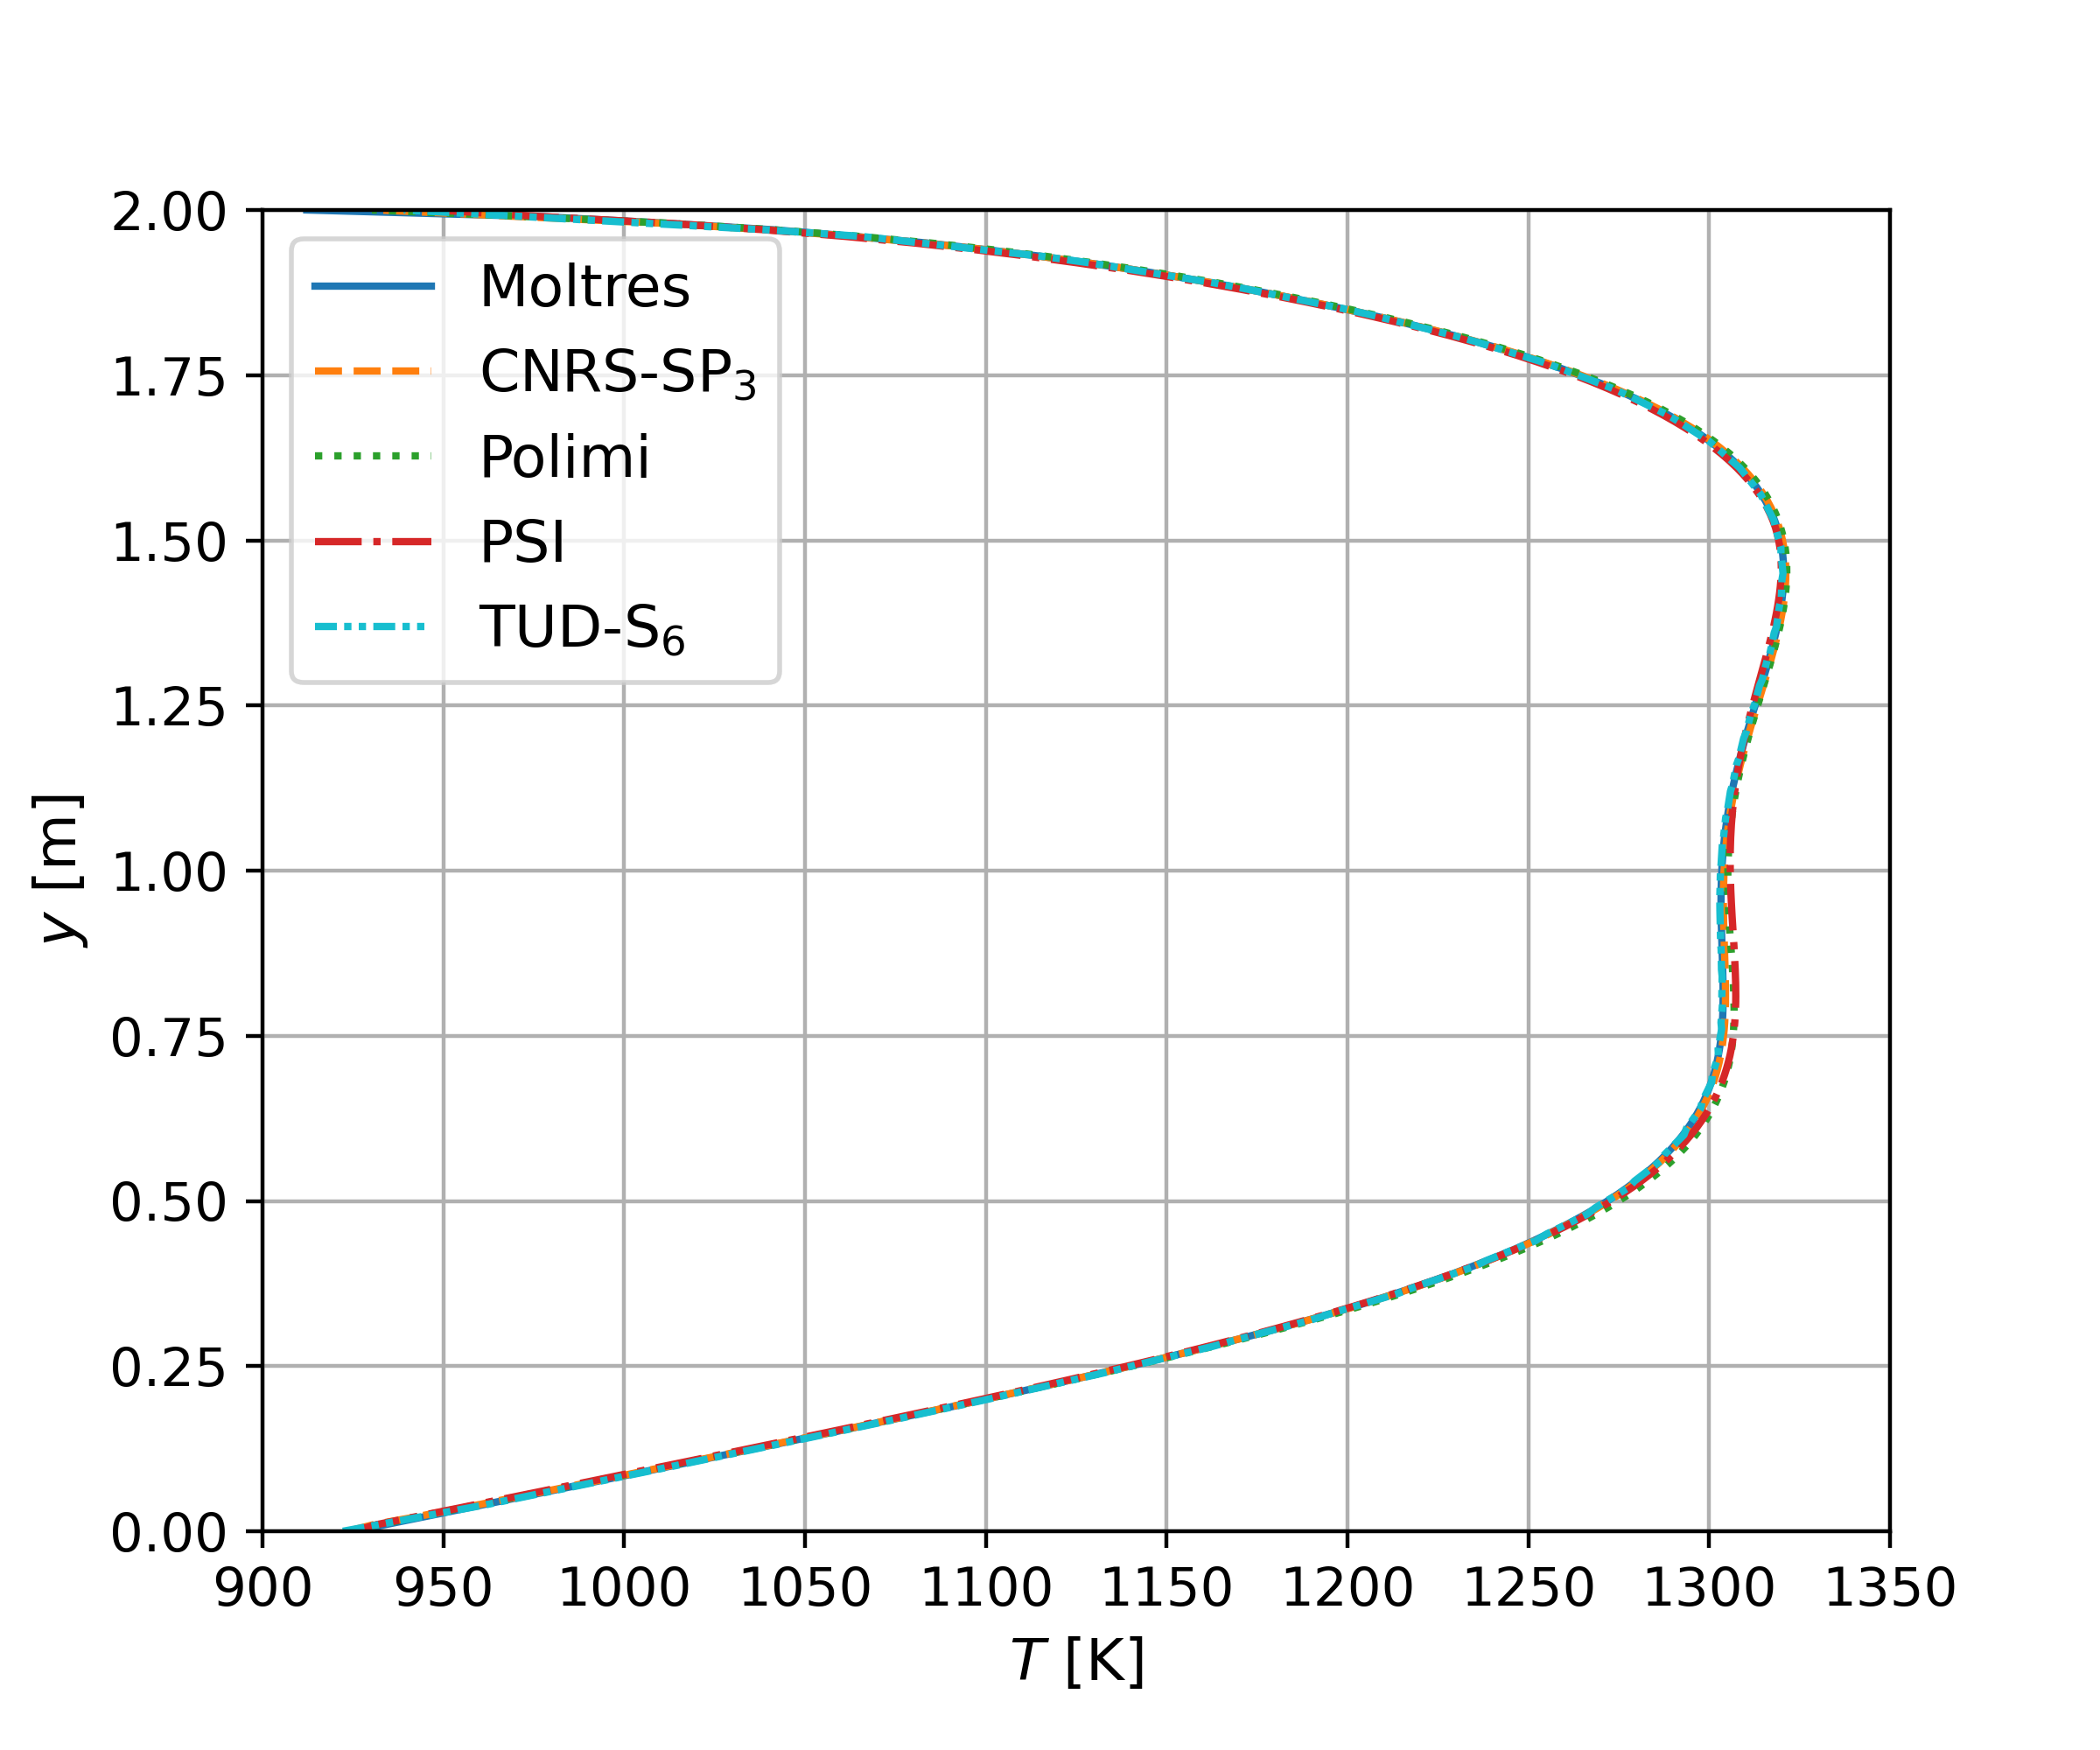
\includegraphics[width=\columnwidth]{0-3-temp-plot}
	  \caption{Step 0.3 \textemdash\ Temperature distribution along BB'.}
	  \label{fig:0.3}
    \end{subfigure}
\end{figure}
%
\FloatBarrier
%
\begin{table}[htb]
	\caption{Discrepancy values from Moltres alongside the average and standard
	deviation of the discrepancy values of the benchmark participants for Phase
	0.}
	\centering
	\small
	\begin{tabular}{l l c S S S}
		\toprule
		\multirow{2}{*}{\textbf{Step}} & \multirow{2}{*}{\textbf{Observable}} & \multirow{2}{*}{\textbf{Centerline}} & {\multirow{2}{*}{\textbf{Moltres [\%]}}} & \multicolumn{2}{c}{\textbf{Benchmark [\%]}} \\
		& & & & {Average} & {SD} \\
		\midrule
		\multirow{4}{*}{0.1} &
		\multirow{2}{*}{$u_x$} & AA' & 0.247 & 0.253 & 0.150 \\
		& & BB' & 0.266 & 0.318 & 0.102 \\
		\cmidrule{2-6}
		& \multirow{2}{*}{$u_y$} & AA' & 0.540 & 0.598 & 0.266 \\
		& & BB' & 0.468 & 0.795 & 0.421 \\
		\midrule
		{0.2} &
		{$\sum^6_g \Sigma_{f,g} \phi_g(\vec{r})$} & AA' & 0.313 & 0.285 & 0.153
		\\
		\midrule
		\multirow{2}{*}{0.3} &
		\multirow{2}{*}{$T$} & AA' & 0.090 & 0.085 & 0.031 \\
		& & BB' & 0.164 & 0.083 & 0.027\\
		\bottomrule
	\end{tabular}
	\label{table:disc0}
\end{table}

\subsubsection{Phase 0 results \& discussion}

Figures \ref{fig:0.1}, \ref{fig:0.2}, and \ref{fig:0.3} show that Moltres
accurately reproduced all three sets of results in Phase 0 for the velocity
field, fission rate density, and temperature. Table
\ref{table:disc0} reports the discrepancy values from Moltres for Phase 0 and
the corresponding average and \gls{SD} of the discrepancy values from
the benchmark participants
\cite{tiberga_results_2020}. Moltres performs very well as most discrepancy
values are either lower than or fall within one \gls{SD} of the benchmark
average discrepancies. The discrepancy value for $T$ along centerline BB' in
Step 0.3 is the only exception, with its value of 0.164\% being larger than
the benchmark average by 3 \gls{SD}.

Figure \ref{fig:0.3} shows that the $T$ distribution from Moltres is almost
identical to the corresponding distributions from CNRS-$SP_3$ and TUD-$S_6$
along most of centerline BB'. However, Figure \ref{fig:0.3-zoom} shows a
significant spread in the $T$ distributions along BB' from all software
packages near the top boundary. At $y = 2.0$ m, Moltres underpredicts the
temperature at 912.3 K compared to the benchmark participants' values which
range between 930.3 K and 948.1 K. This point on the top boundary lies directly downstream of
the velocity boundary condition discontinuity at the top-left corner.
Corner singularities are generally tricky to approximate with
continuous Galerkin methods \cite{kuhlmann_lid-driven_2018}.
The \gls{SUPG} stabilization scheme dampens numerical oscillations by
introducing pointwise artificial thermal diffusivity, which depends strongly on
the inverse of local velocity magnitude \cite{peterson_overview_2018}.
Therefore, while the \gls{SUPG} scheme effectively eliminates
spurious numerical oscillations everywhere else, it provides little damping
along the top boundary due to the relatively large non-zero velocity boundary
condition. On the other hand, the temperature values in the rest of the domain
and the average discrepancies of the other variables show that Moltres can
still accurately reproduce the expected results, and the temperature deviations
along the top boundary do not impact the overall integrity of our results.

\begin{figure}[htb]
	\centering
	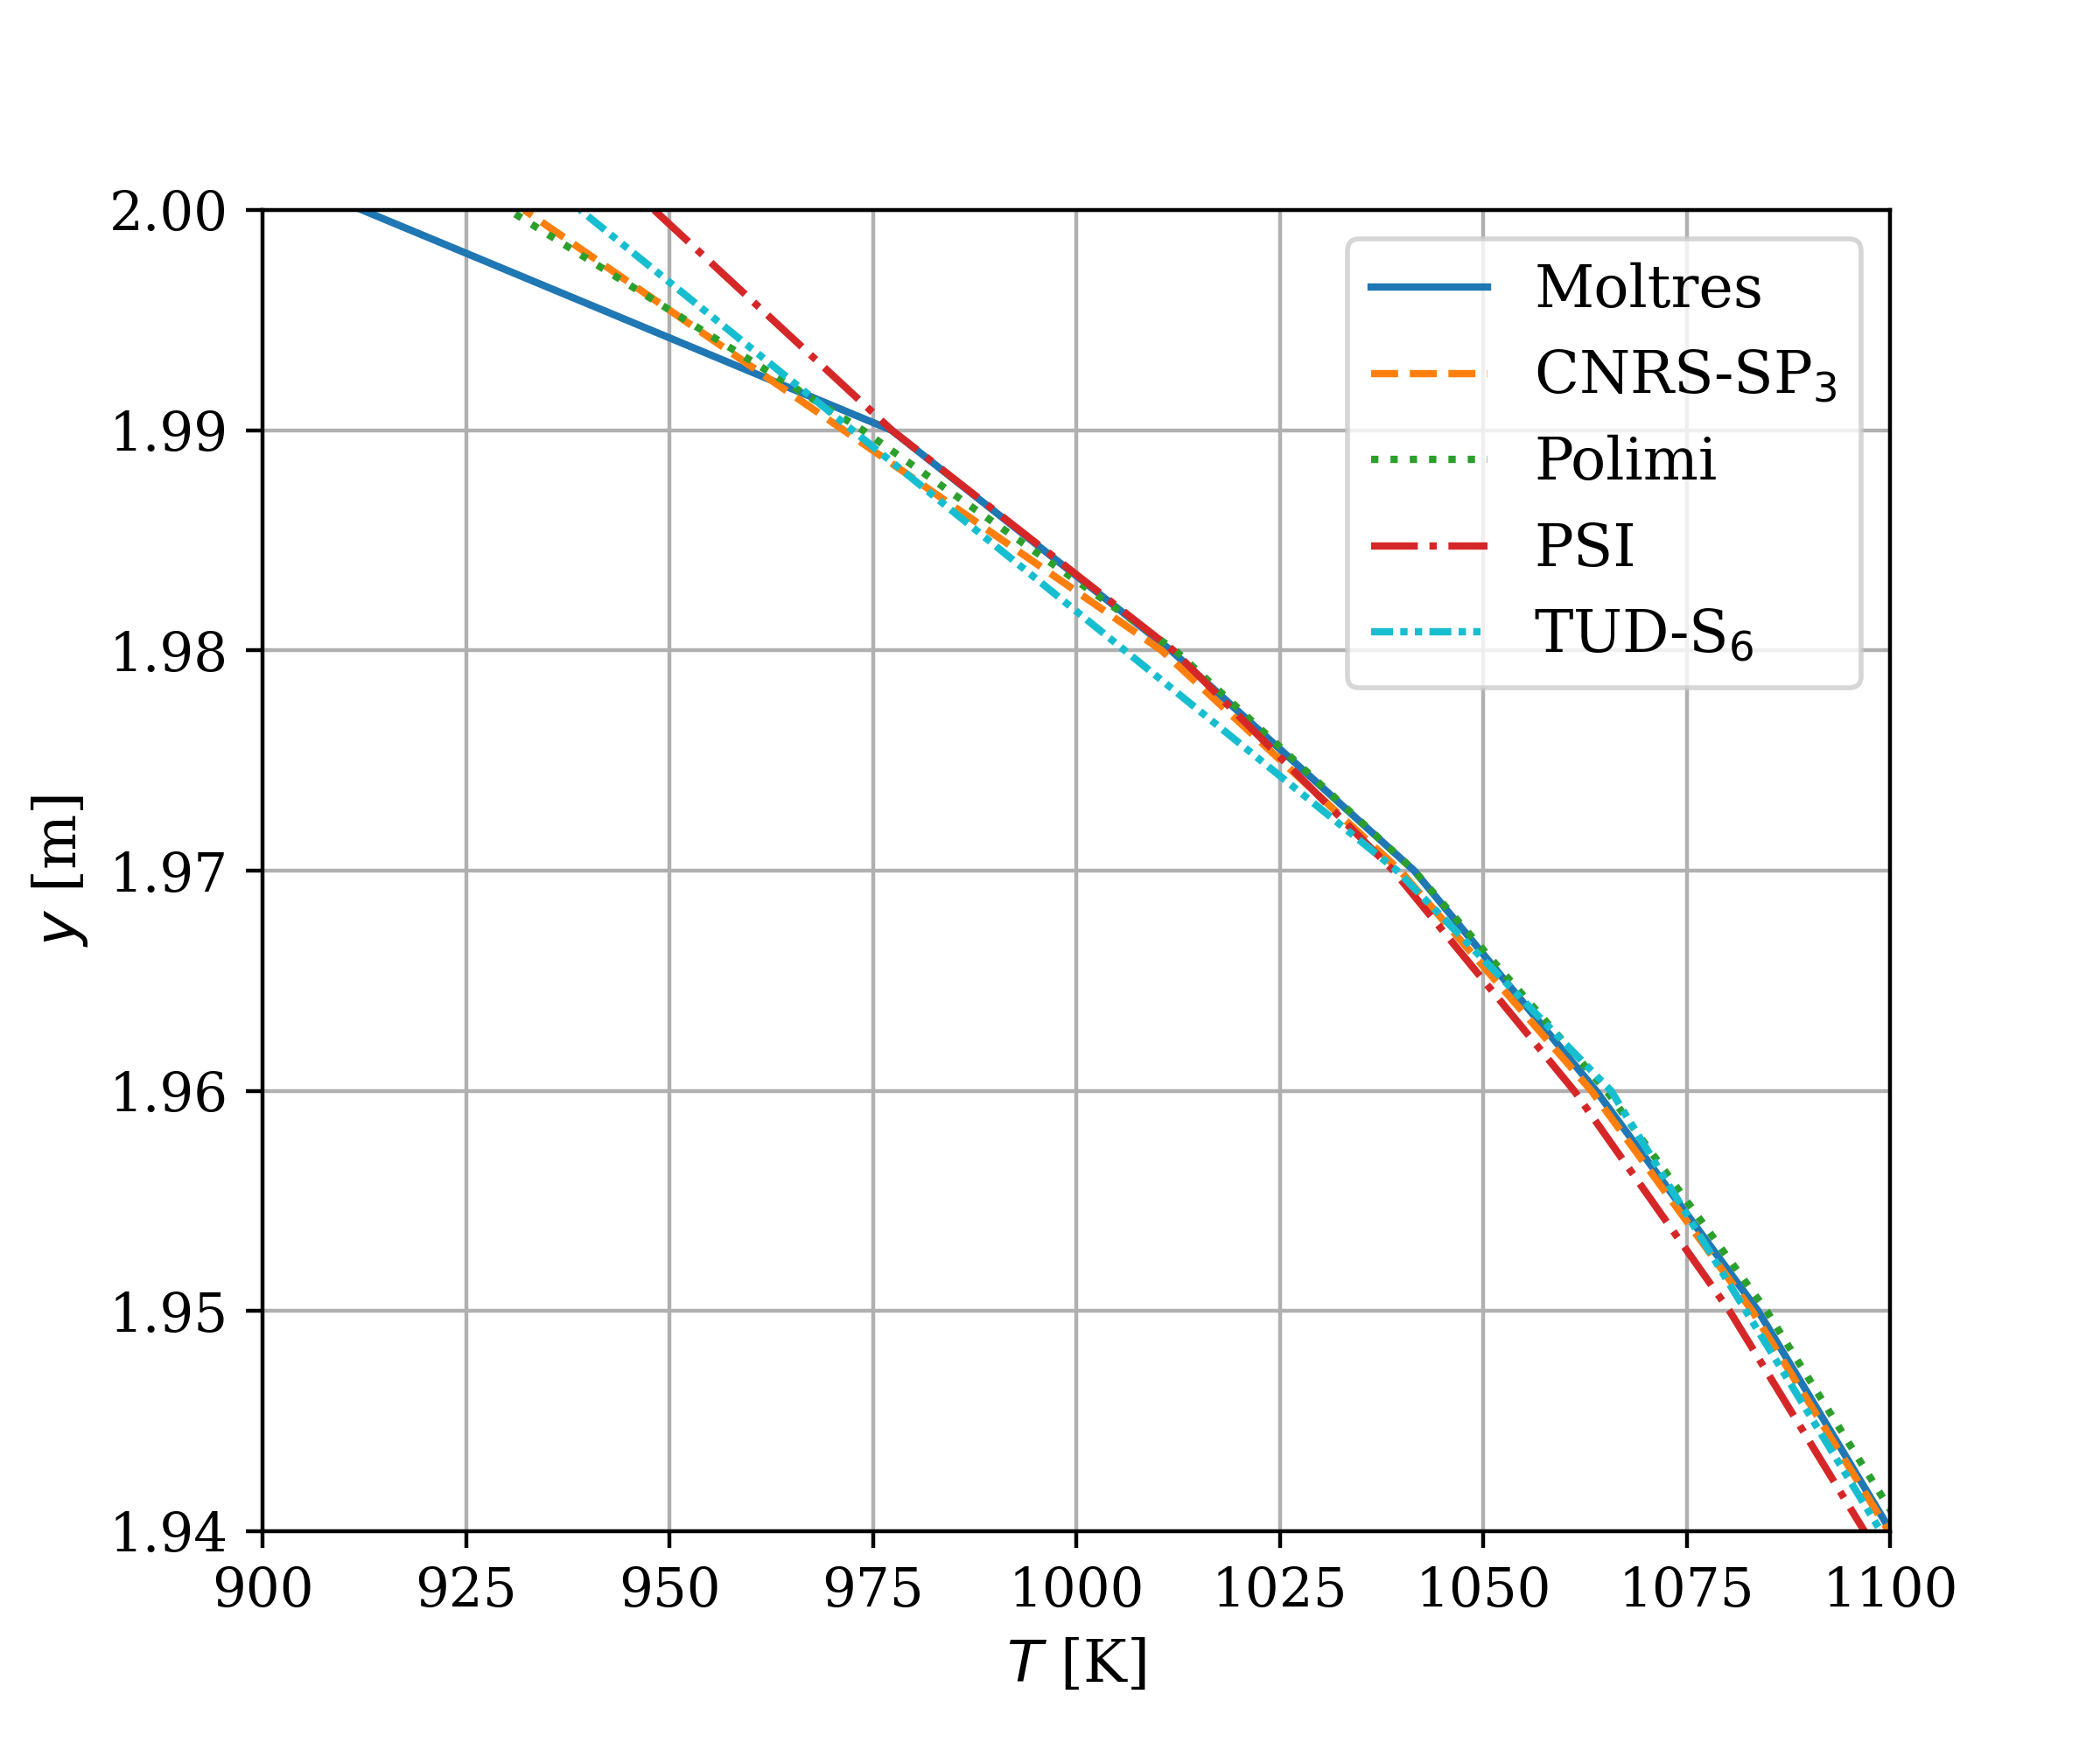
\includegraphics[width=.49\columnwidth]{0-3-temp-plot-zoom}
	\caption{Step 0.3 \textemdash\ Temperature distribution along BB' for y = 1.94 m to
	y = 2.00 m.}
	\label{fig:0.3-zoom}
\end{figure}

Lastly, we observe in table \ref{table:rho} that the reactivity $\rho$ value of
465.6 pcm from Moltres falls well within the range of $\rho$ values from the
benchmark, which range from 353.7 pcm up to 578.1 pcm. Given that Moltres 
adopts the neutron diffusion model, our $\rho$ value agrees closest to the
results from the software packages which also adopt the neutron diffusion model
or theoretically-equivalent models such as the $SP_1$ and $S_2$ neutron
transport models, namely CNRS-$SP_1$, PoliMi, PSI, and TUD-$S_2$.

\begin{table}[htb]
    \caption{Reactivity $\rho$ and change in reactivity
    $\left(\rho_a - \rho_b\right)$ values from Steps 0.2, 1.1,
    1.2, and 1.3. All units are in pcm.}
    \centering
    \small
    \setlength\tabcolsep{2pt}
    \begin{tabular}{l S S S S}
        \toprule
        \multirow{2}{*}{\textbf{Software}} & {\textbf{Step 0.2}} &
        {\textbf{Step 1.1}} & {\textbf{Step 1.2}} & {\textbf{Step 1.3}} \\
        & {$\rho_{s_{0.2}}$}
        & {$\rho_{s_{1.1}} - \rho_{s_{0.2}}$}
        & {$\rho_{s_{1.2}} - \rho_{s_{1.1}}$}
        & {$\rho_{s_{1.3}} - \rho_{s_{0.2}}$} \\
        \midrule
        Moltres     & 465.6 & -62.7 & -1142.2 & -1207.7 \\
        CNRS-$SP_1$ & 411.3 & -62.5 & -1152.0 & -1220.5 \\
        CNRS-$SP_3$ & 353.7 & -62.6 & -1152.7 & -1220.7 \\
        PoliMi      & 421.2 & -62.0 & -1161.0 & -1227.0 \\
        PSI         & 411.7 & -63.0 & -1154.8 & -1219.6 \\
        TUD-$S_2$   & 482.6 & -62.0 & -1145.2 & -1208.5 \\
        TUD-$S_6$   & 578.1 & -60.7 & -1122.0 & -1184.4 \\
        \bottomrule
    \end{tabular}
    \label{table:rho}
\end{table}

\FloatBarrier

\subsubsection{Phase 1 results \& discussion}

Table \ref{table:disc1} shows the discrepancy values from Moltres relative to
the average and \gls{SD} of the benchmark participants for Steps 1.1, 1.2, and
1.3 and the corresponding average discrepancy values from the benchmark
\cite{tiberga_results_2020}. The subsequent subsections discuss the results
for each benchmark step in Phase 1.
%
\begin{table}[htb]
	\caption{Discrepancy values from Moltres alongside the average and standard
	deviation of the discrepancy values of the benchmark participants for Phase
	1.}
	\centering
	\small
	\begin{tabular}{l l c S S S}
		\toprule
		\multirow{2}{*}{\textbf{Step}} & \multirow{2}{*}{\textbf{Observable}} & \multirow{2}{*}{\textbf{Centerline}} & {\multirow{2}{*}{\textbf{Moltres [\%]}}} & \multicolumn{2}{c}{\textbf{Benchmark [\%]}} \\
		& & & & {Average} & {SD} \\
		\midrule
		\multirow{2}{*}{1.1} &
		\multirow{2}{*}{$\sum_i \lambda_i C_i$} & AA' & 0.603 & 0.346 & 0.166
		\\
		& & BB' & 0.327 & 0.294 & 0.153 \\
		\midrule
		\multirow{4}{*}{1.2} &
		\multirow{2}{*}{$T$} & AA' & 0.076 & 0.095 & 0.015 \\
		& & BB' & 0.179 & 0.089 & 0.012 \\
		\cmidrule{2-6}
		& \multirow{2}{*}{\footnotesize $\Delta\left[\sum^6_g \Sigma_{f,g} \phi_g(\vec{r})
		\right]_{s_{1.2}-s_{0.2}}$} & AA' & 1.110 & 1.576 & 0.564 \\
		& & BB' & 1.089 & 1.133 & 0.392 \\
		\midrule
		\multirow{7}{*}{1.3} &
		{$u_x$} & AA' & 0.123 & 0.691 & 0.566 \\
		\cmidrule{2-6}
		& \multirow{2}{*}{$u_y$} & AA' & 0.237 & 0.329 & 0.131 \\
		& & BB' & 0.238 & 0.356 & 0.217 \\
		\cmidrule{2-6}
		& \multirow{2}{*}{$T$} & AA' & 0.064 & 0.057 & 0.023 \\
		& & BB' & 0.070 & 0.080 & 0.024 \\
		\cmidrule{2-6}
		& \multirow{2}{*}{$\sum_i \lambda_i C_i$} & AA' & 1.043 & 0.460 & 0.190
		\\
		& & BB' & 0.462 & 1.194 & 0.178 \\
		\bottomrule
	\end{tabular}
	\label{table:disc1}
\end{table}

\paragraph{Step 1.1: Circulating fuel}

Figure \ref{fig:1.1} shows good qualitative agreement in the delayed neutron
source distribution along BB' among Moltres and the benchmark participants.
From Table \ref{table:disc1}, Moltres reports discrepancies of 0.603\% and
0.327\% along the centerlines AA' and BB', respectively. Both values are
within two and one \gls{SD}, respectively, of the average discrepancies of the
benchmark participants (0.346\% and 0.294\%).
In Table \ref{table:rho}, we observe that the change in
$\rho$ relative to Step 0.2 is $-62.7$ pcm for Moltres, and this value is
consistent with the $-63.0$ to $-62.0$ pcm range that most of the benchmark
participants' values fall in.
%
\begin{figure}[htb]
	\centering
    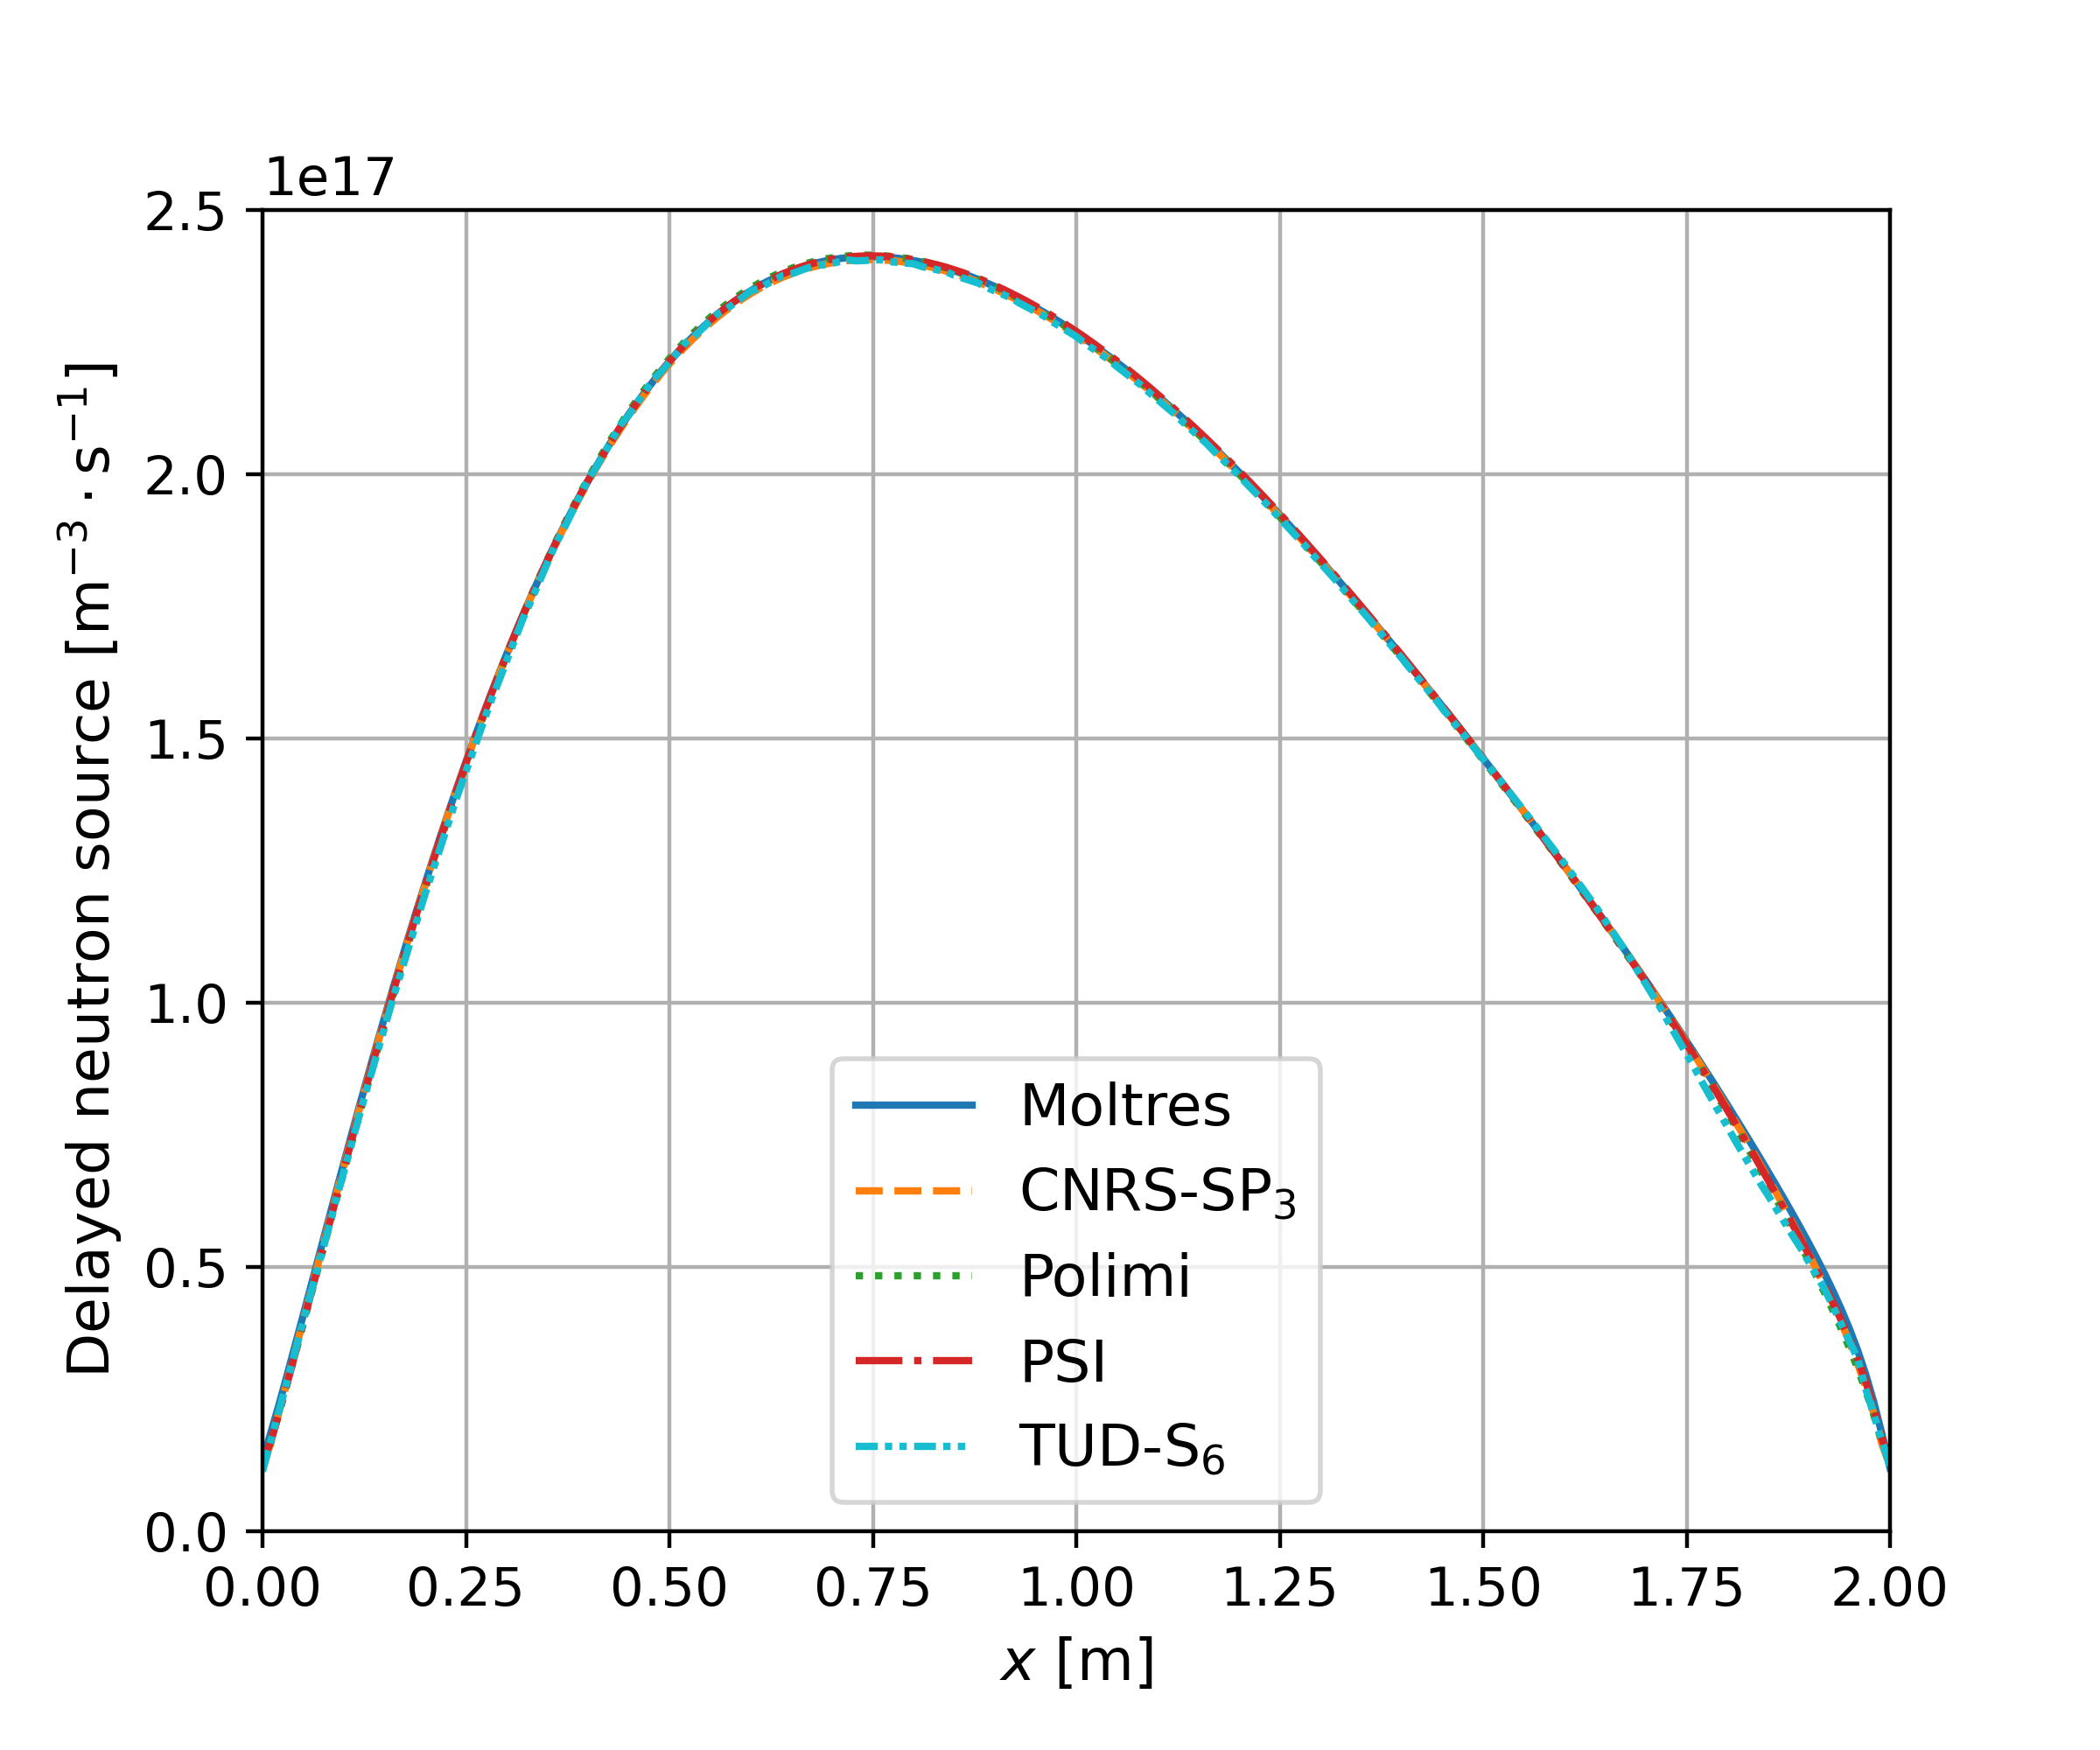
\includegraphics[width=.49\columnwidth]{1-1-dnp-x-plot}
    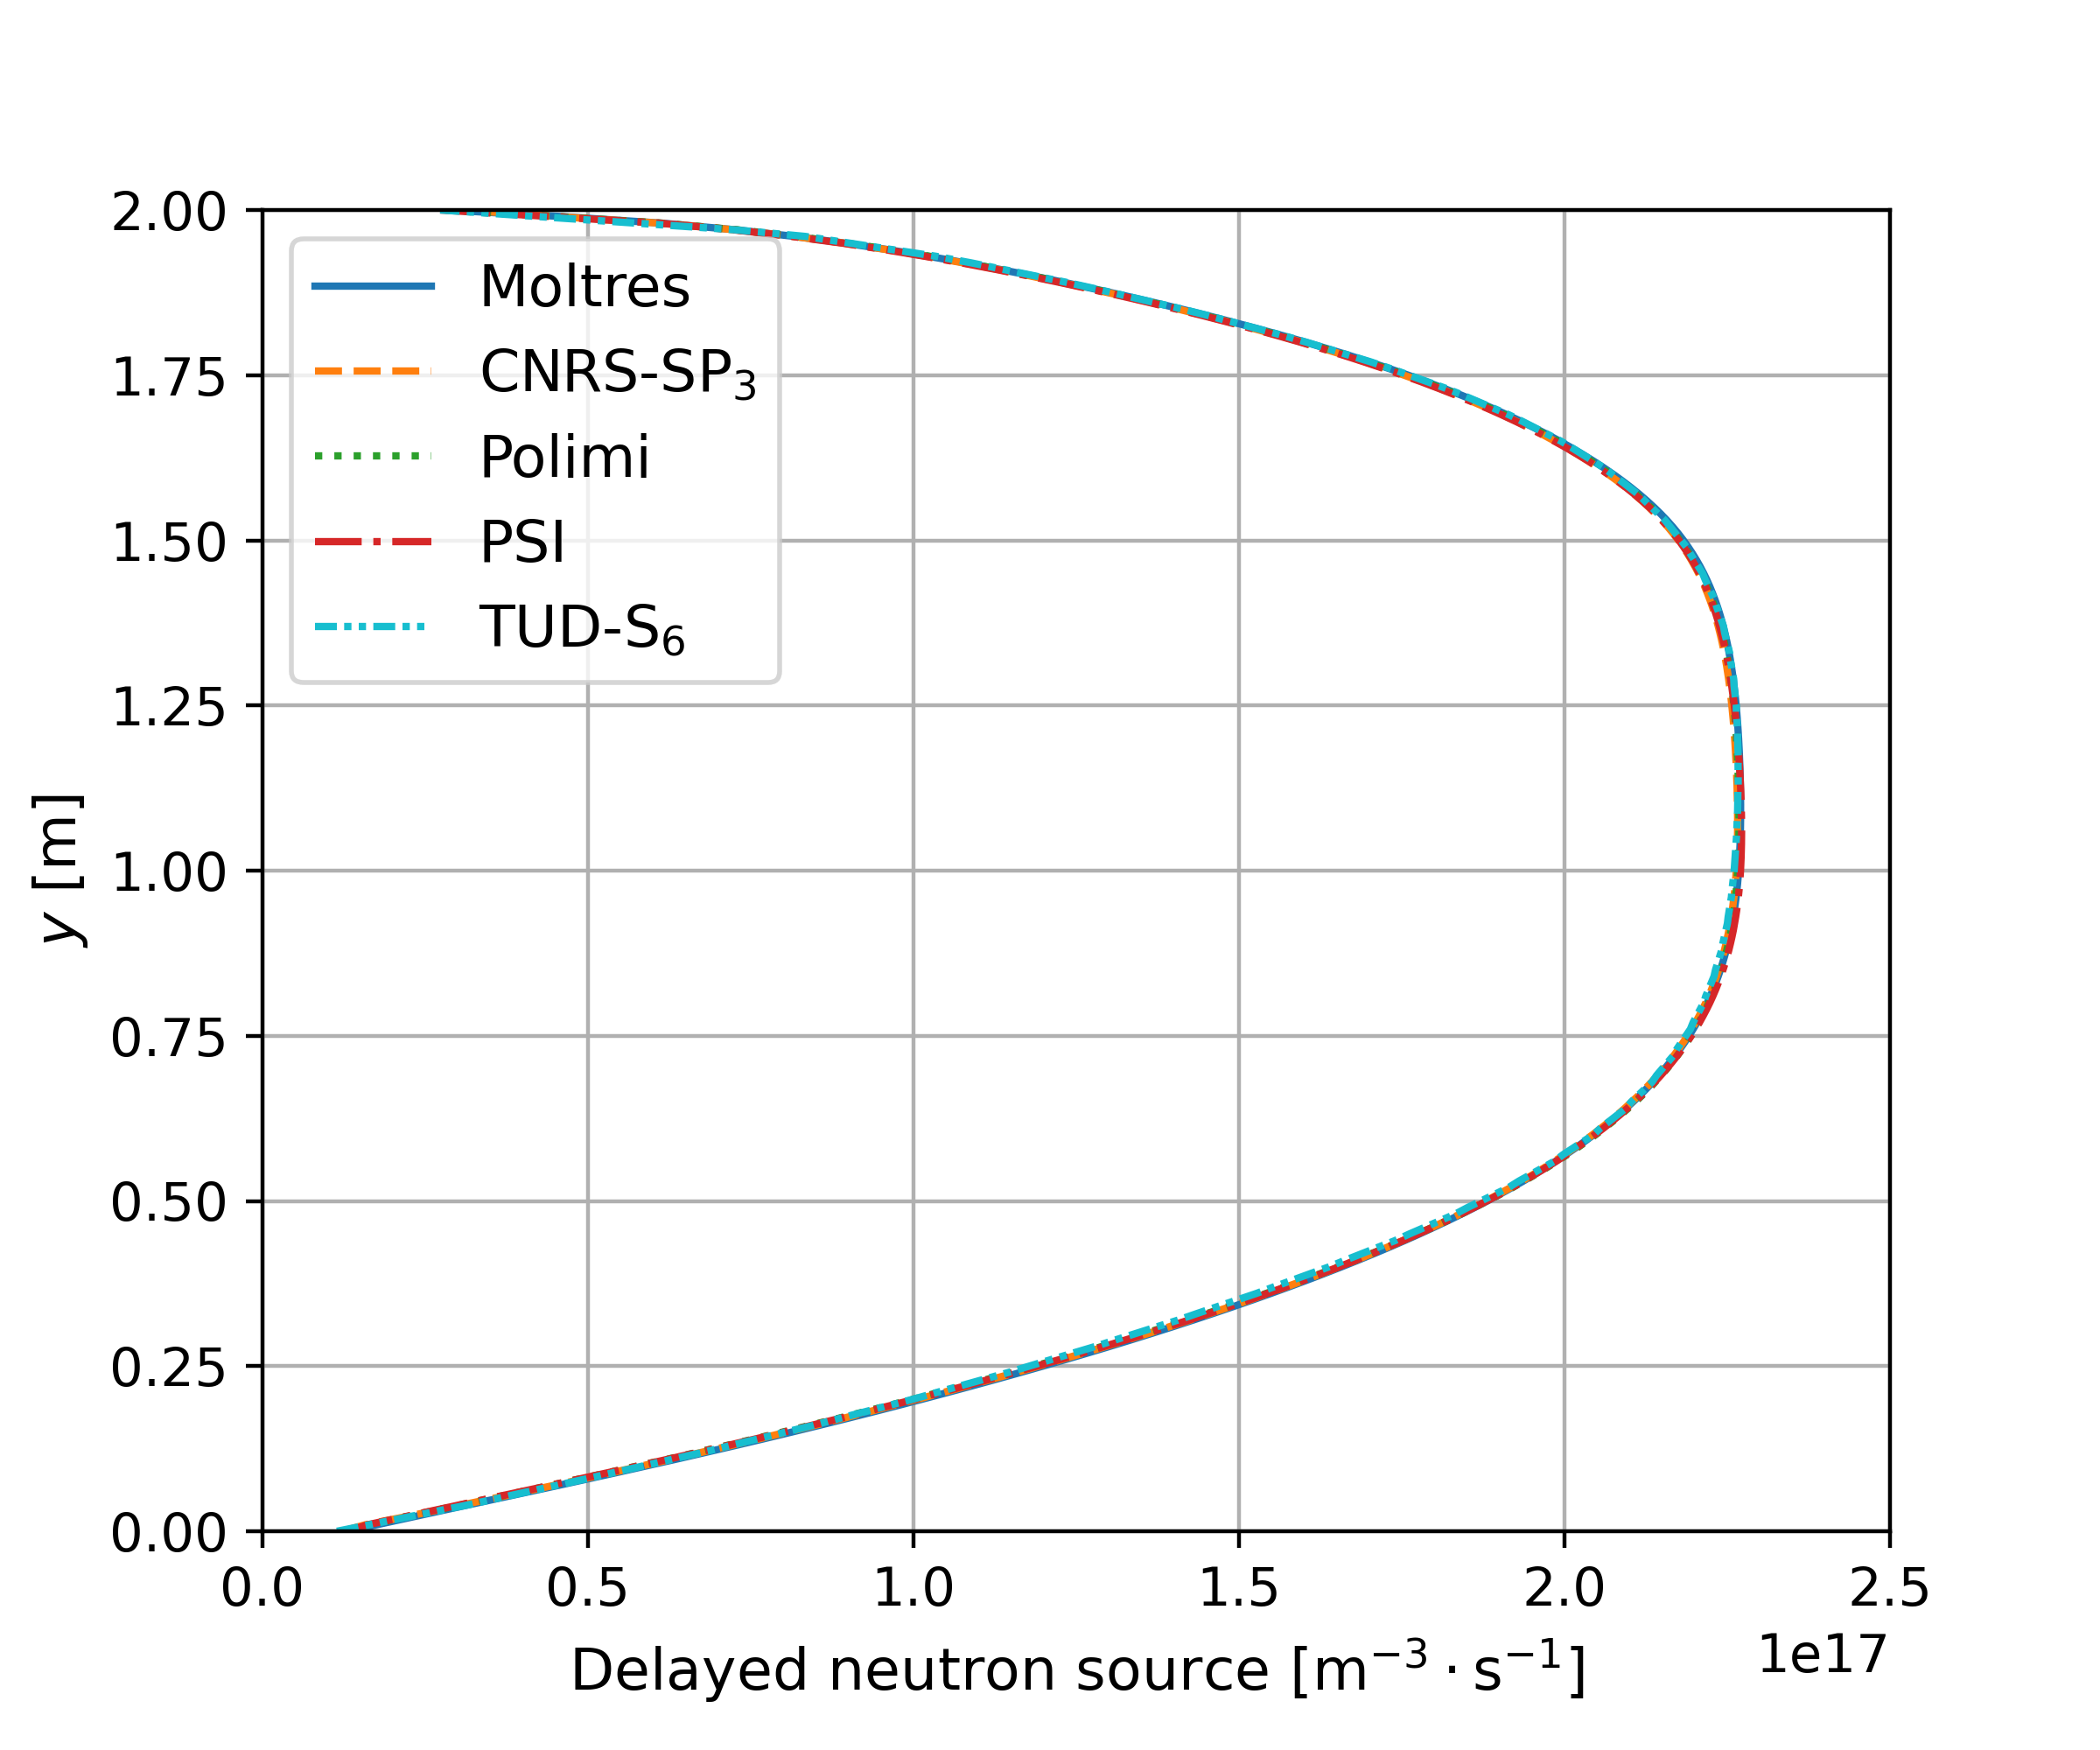
\includegraphics[width=.49\columnwidth]{1-1-dnp-y-plot}
	\caption{Step 1.1 \textemdash\ Delayed neutron source along AA' (top) and BB'
	(bottom).}
	\label{fig:1.1}
\end{figure}
%
\begin{figure}[htb]
	\centering
	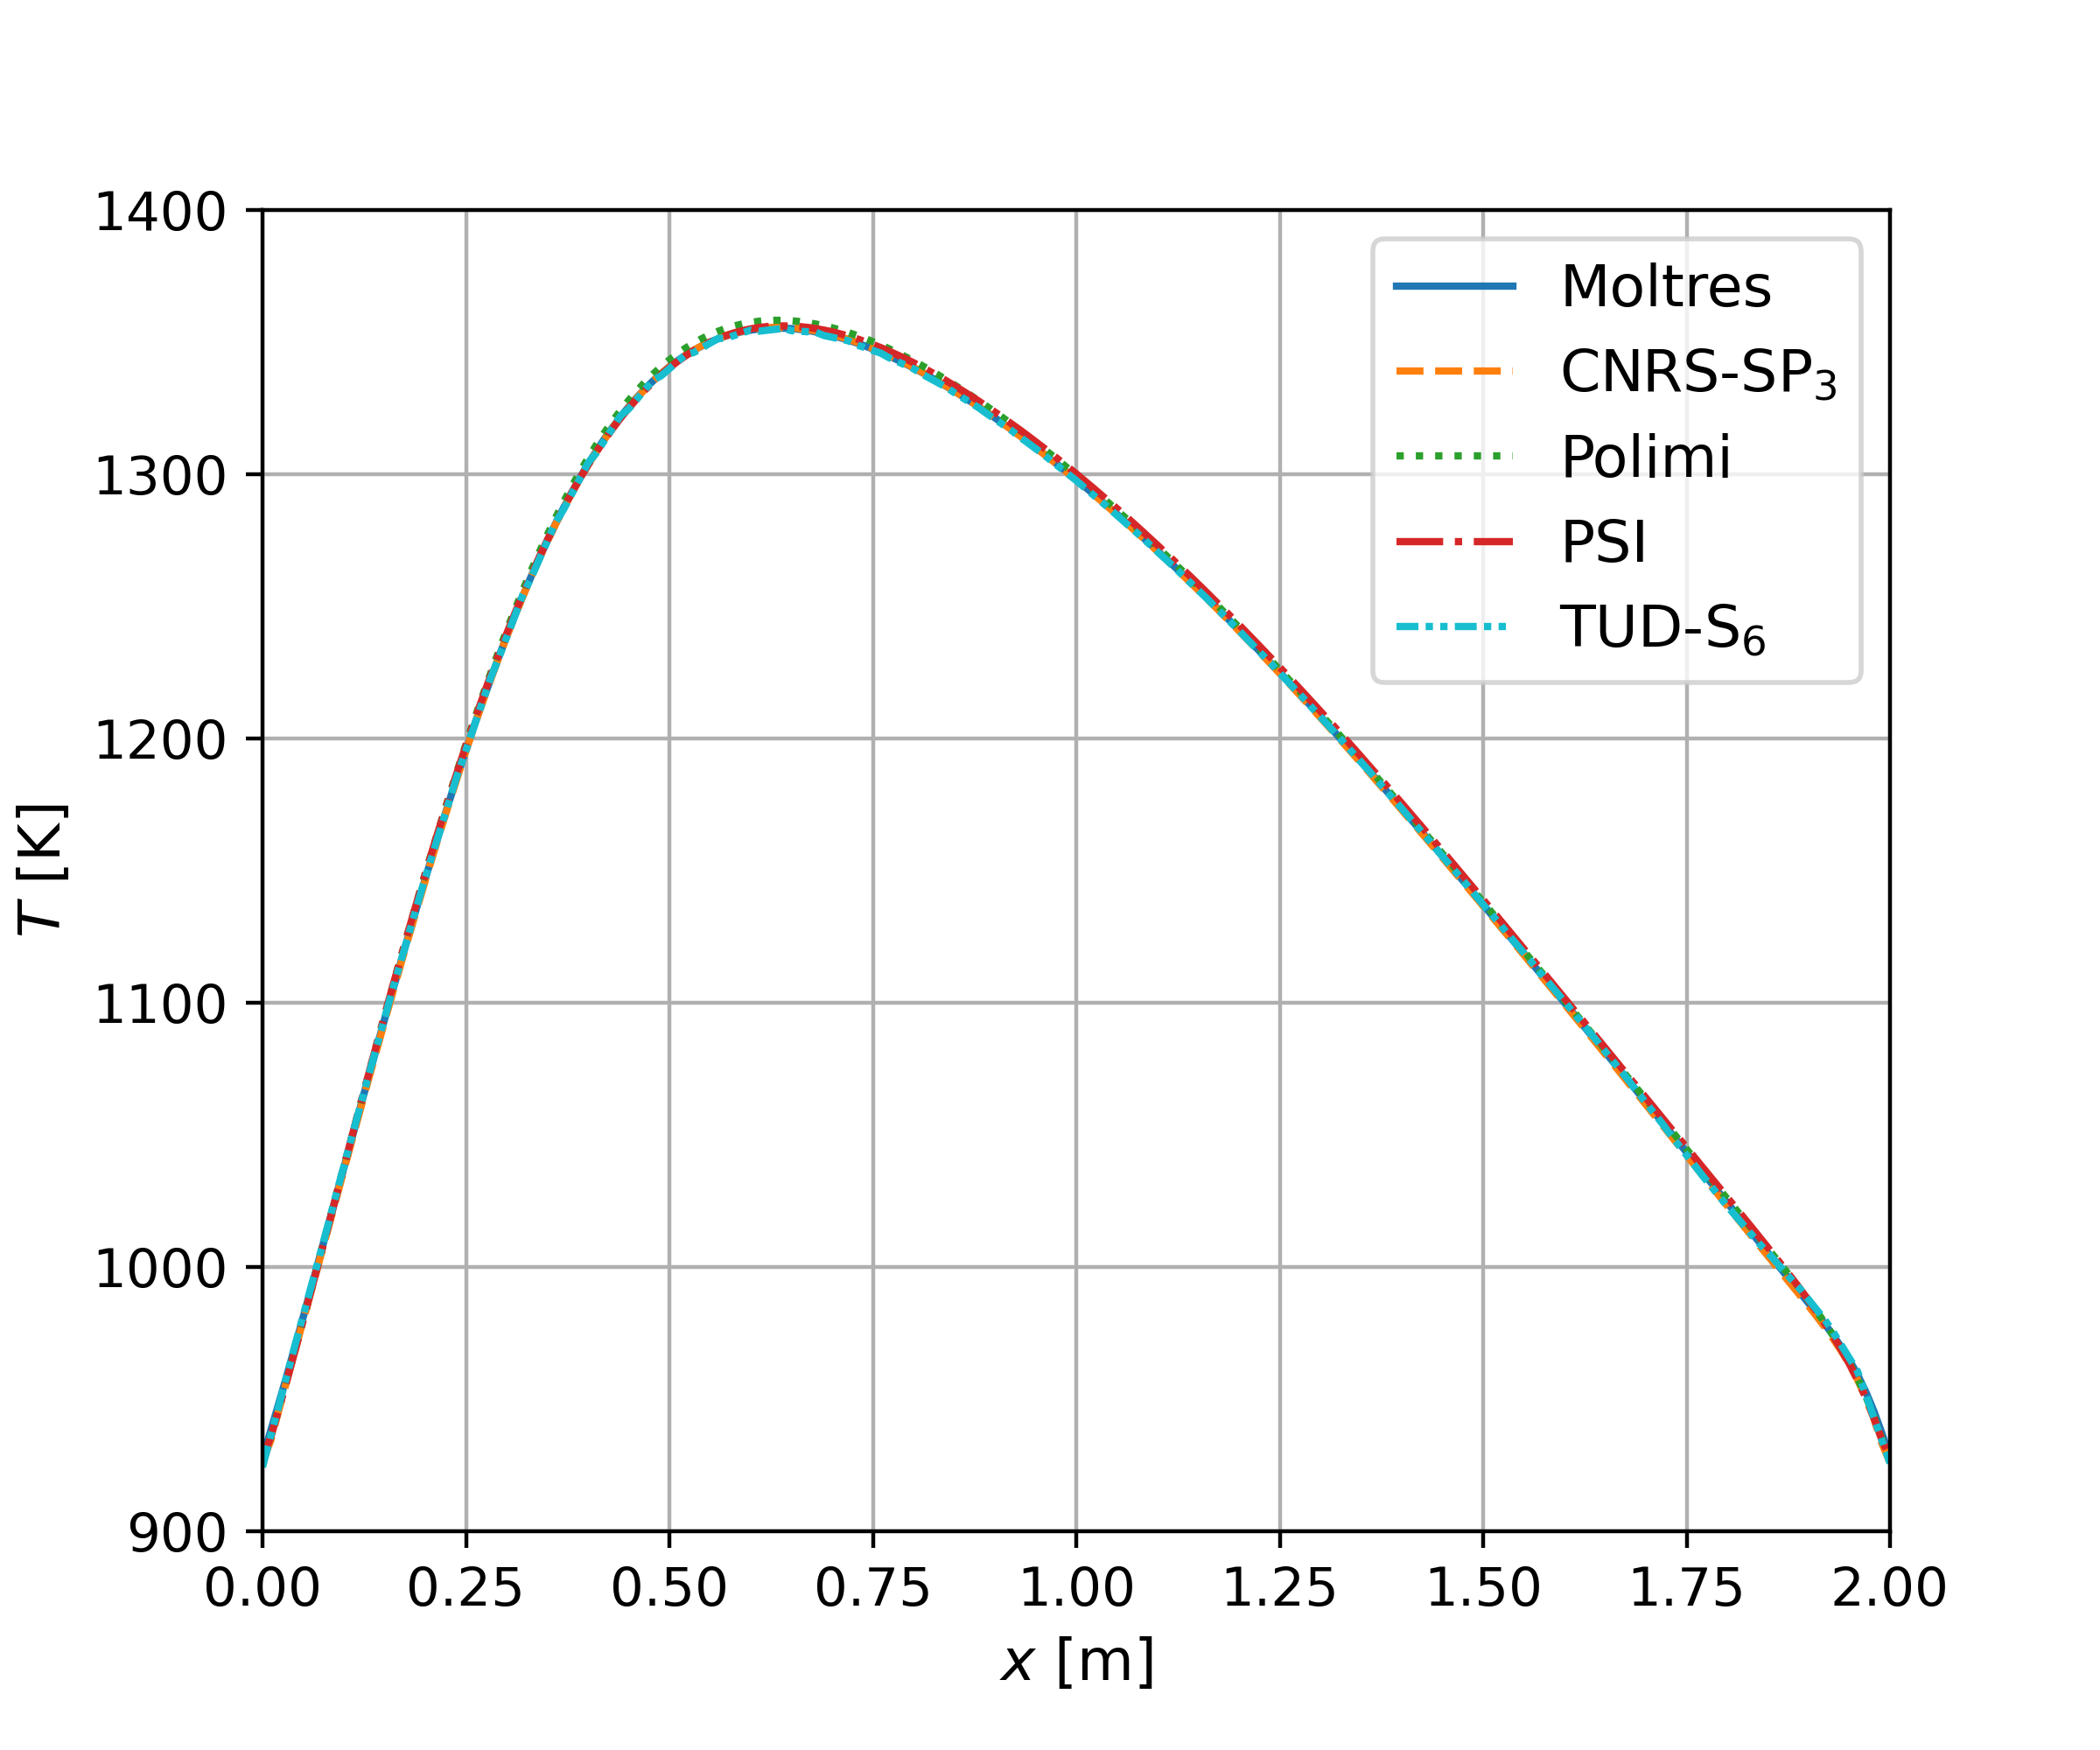
\includegraphics[width=.49\columnwidth]{1-2-temp-plot}
	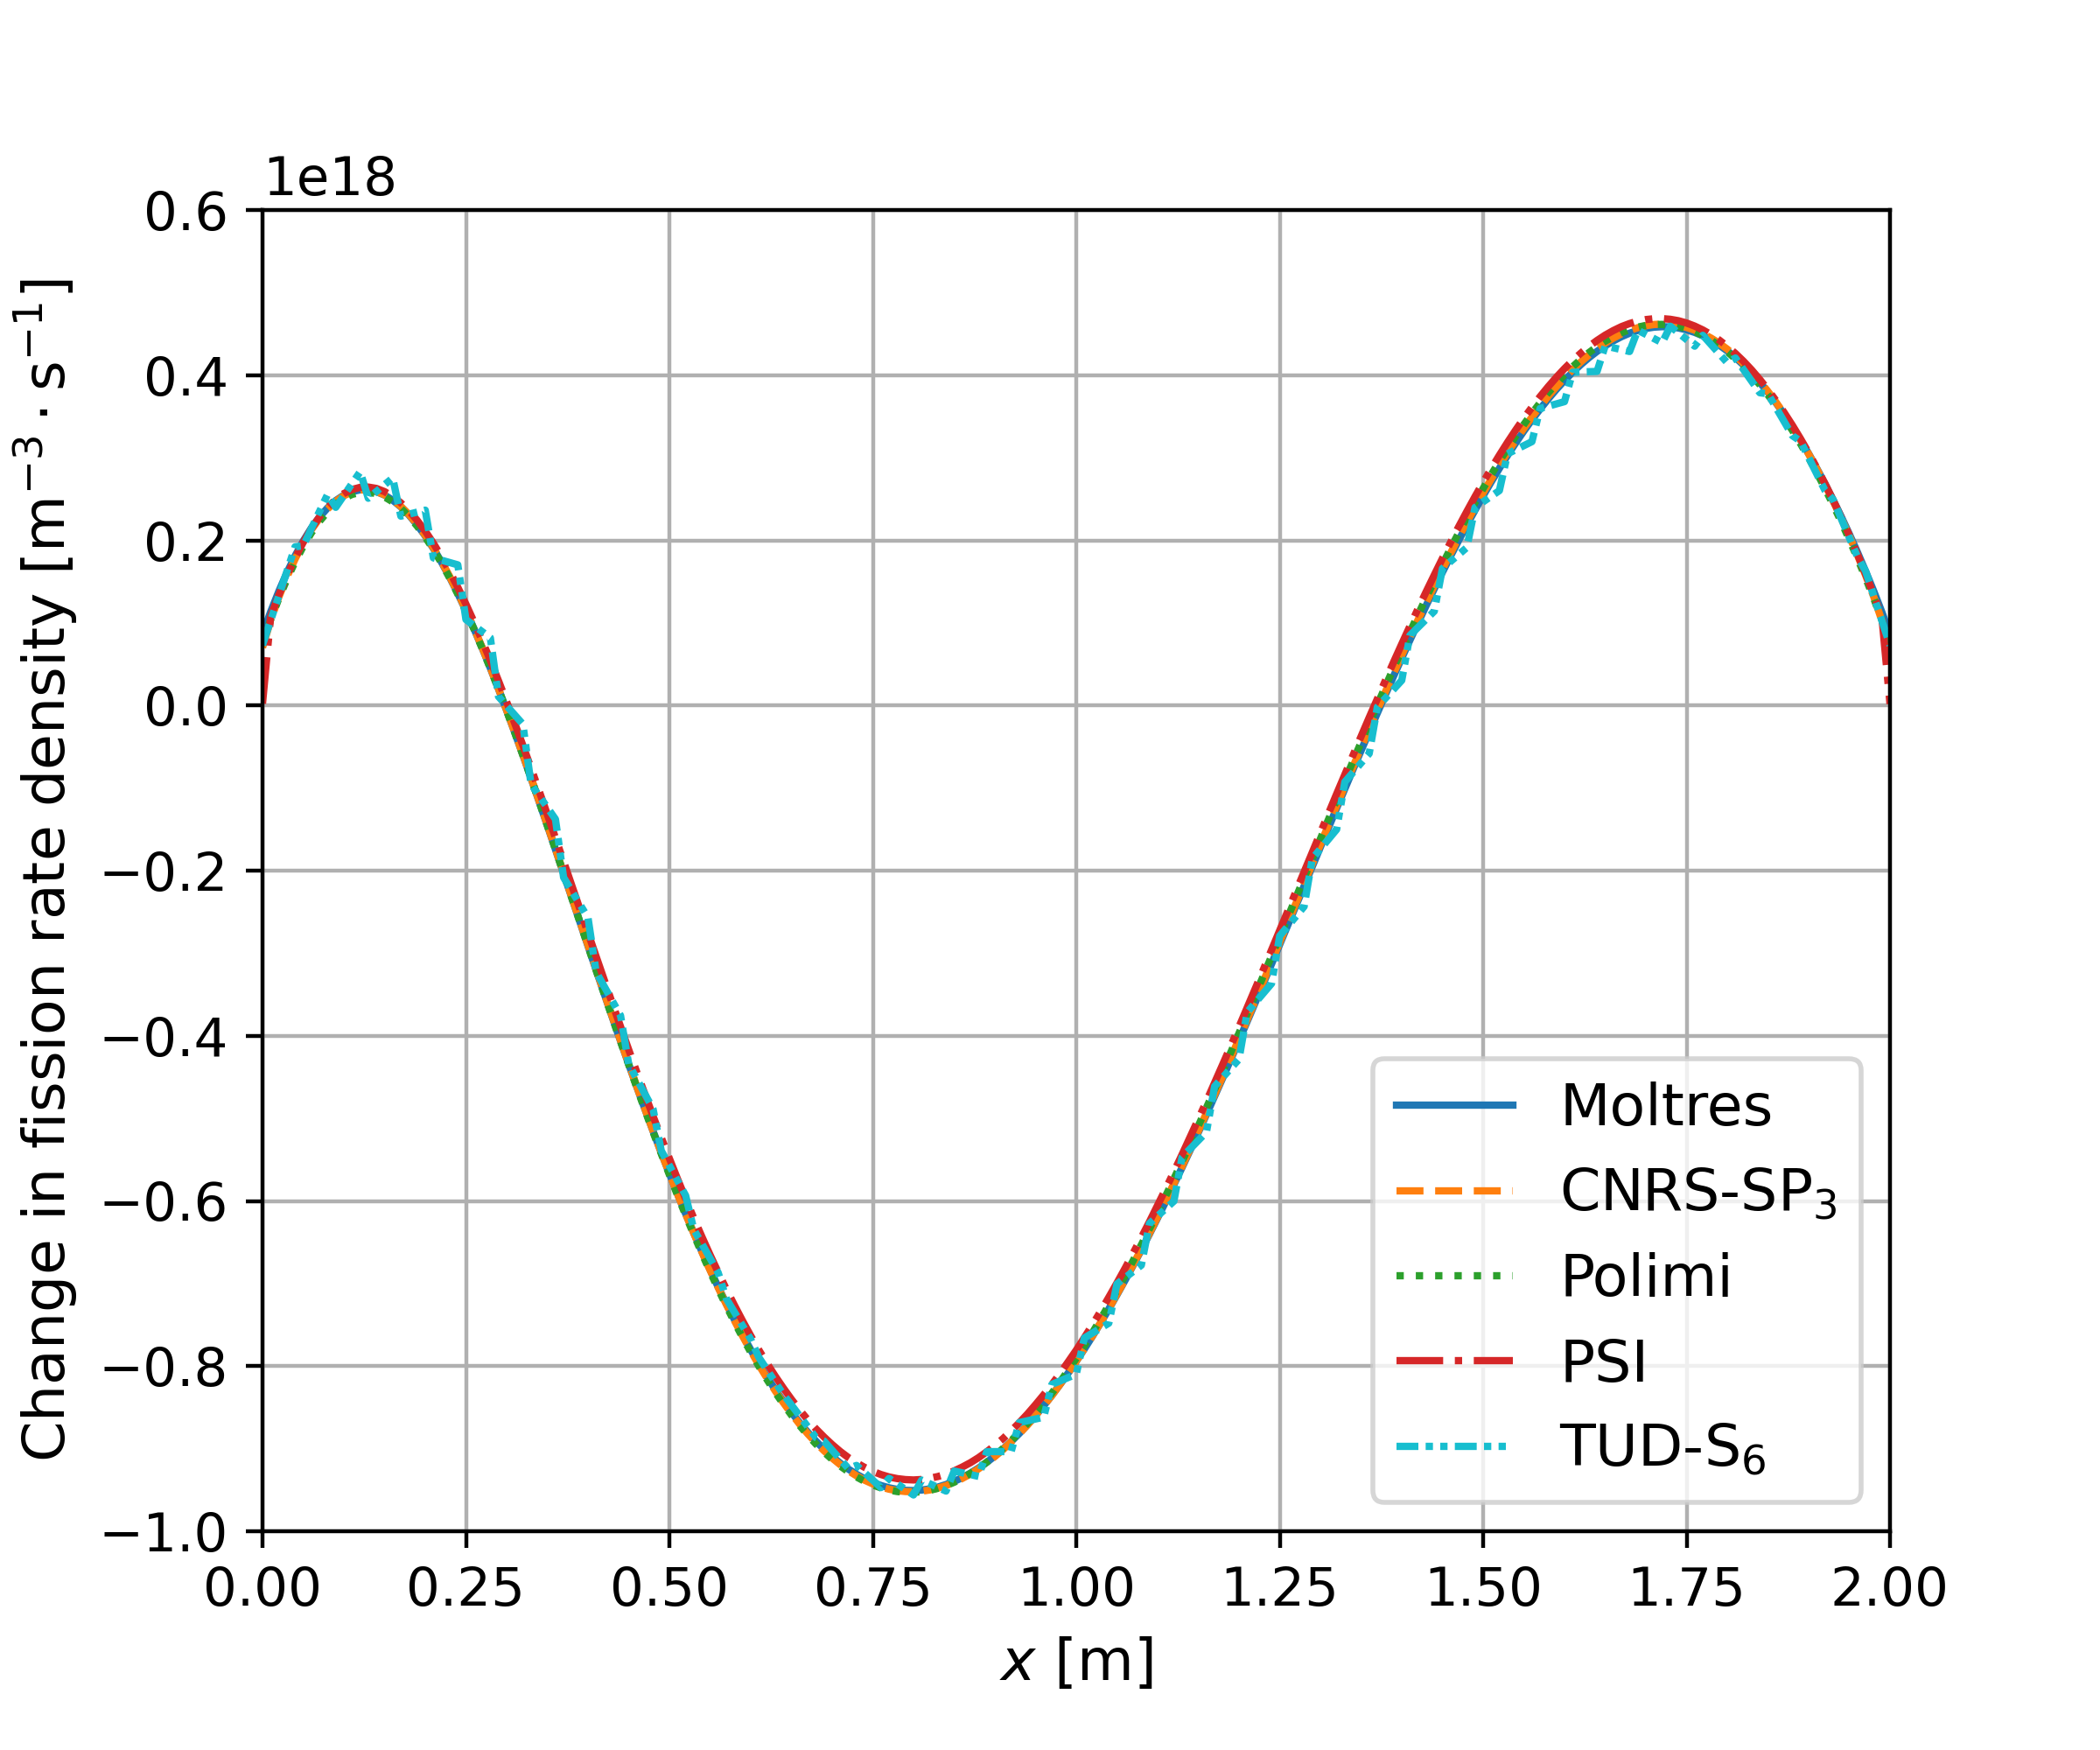
\includegraphics[width=.49\columnwidth]{1-2-fiss-plot}
	\caption{Step 1.2 \textemdash\ Temperature distribution and change in fission rate
	density along AA'.}
	\label{fig:1.2}
\end{figure}

\FloatBarrier

\paragraph{Step 1.2: Power coupling}

Figure \ref{fig:1.2} shows the temperature distribution and the change in
fission rate density along AA' from Step 1.2. Similar to Step 0.3, the
temperature distribution from Moltres agrees closest with CNRS-$SP_3$ and
TUD-$S_2$. Table \ref{table:disc1} reports the same trends we observed in Phase
0; the average discrepancy in temperature along BB' from Moltres for Step 1.2
is marginally higher than the benchmark, while the average discrepancy in the
fission rate density is within one \gls{SD} range to the benchmark average.
From Table \ref{table:rho}, Moltres also reports a change in $\rho$
relative to Step 1.1 of $-1142.2$ pcm, which
falls within the range of reported benchmark participants' values.

\paragraph{Step 1.3: Buoyancy}

Figure \ref{fig:1.3} shows the vertical velocity component, temperature, and
delayed neutron source distributions along AA'.
Moltres reproduces the correct trend in all three physical
observables. Step 1.3 has a relatively slower buoyancy-driven flow profile with
no forced flow from the top boundary. Consequently, there are no temperature
deviations near the top boundary, and we observe in Table \ref{table:disc1} that
the average discrepancy value of 0.070\% for the temperature distribution along
BB' is in much closer agreement to the benchmark value of 0.080\% compared to
the corresponding temperature discrepancy values for Step 0.3 and 1.2.

Table \ref{table:rho} shows that the change in $\rho$ from
Moltres (-1207.7 pcm) falls within the range of reported benchmark values and
matches the software from TUD-$S_2$ (-1208.5 pcm) the closest. This observation is likely
due to the similar solvers (diffusion and $S_2$ neutronics models) and
methods of solution (finite element method on uniform meshes) employed by our
respective software.
%
\begin{figure}[htb]
	\centering
	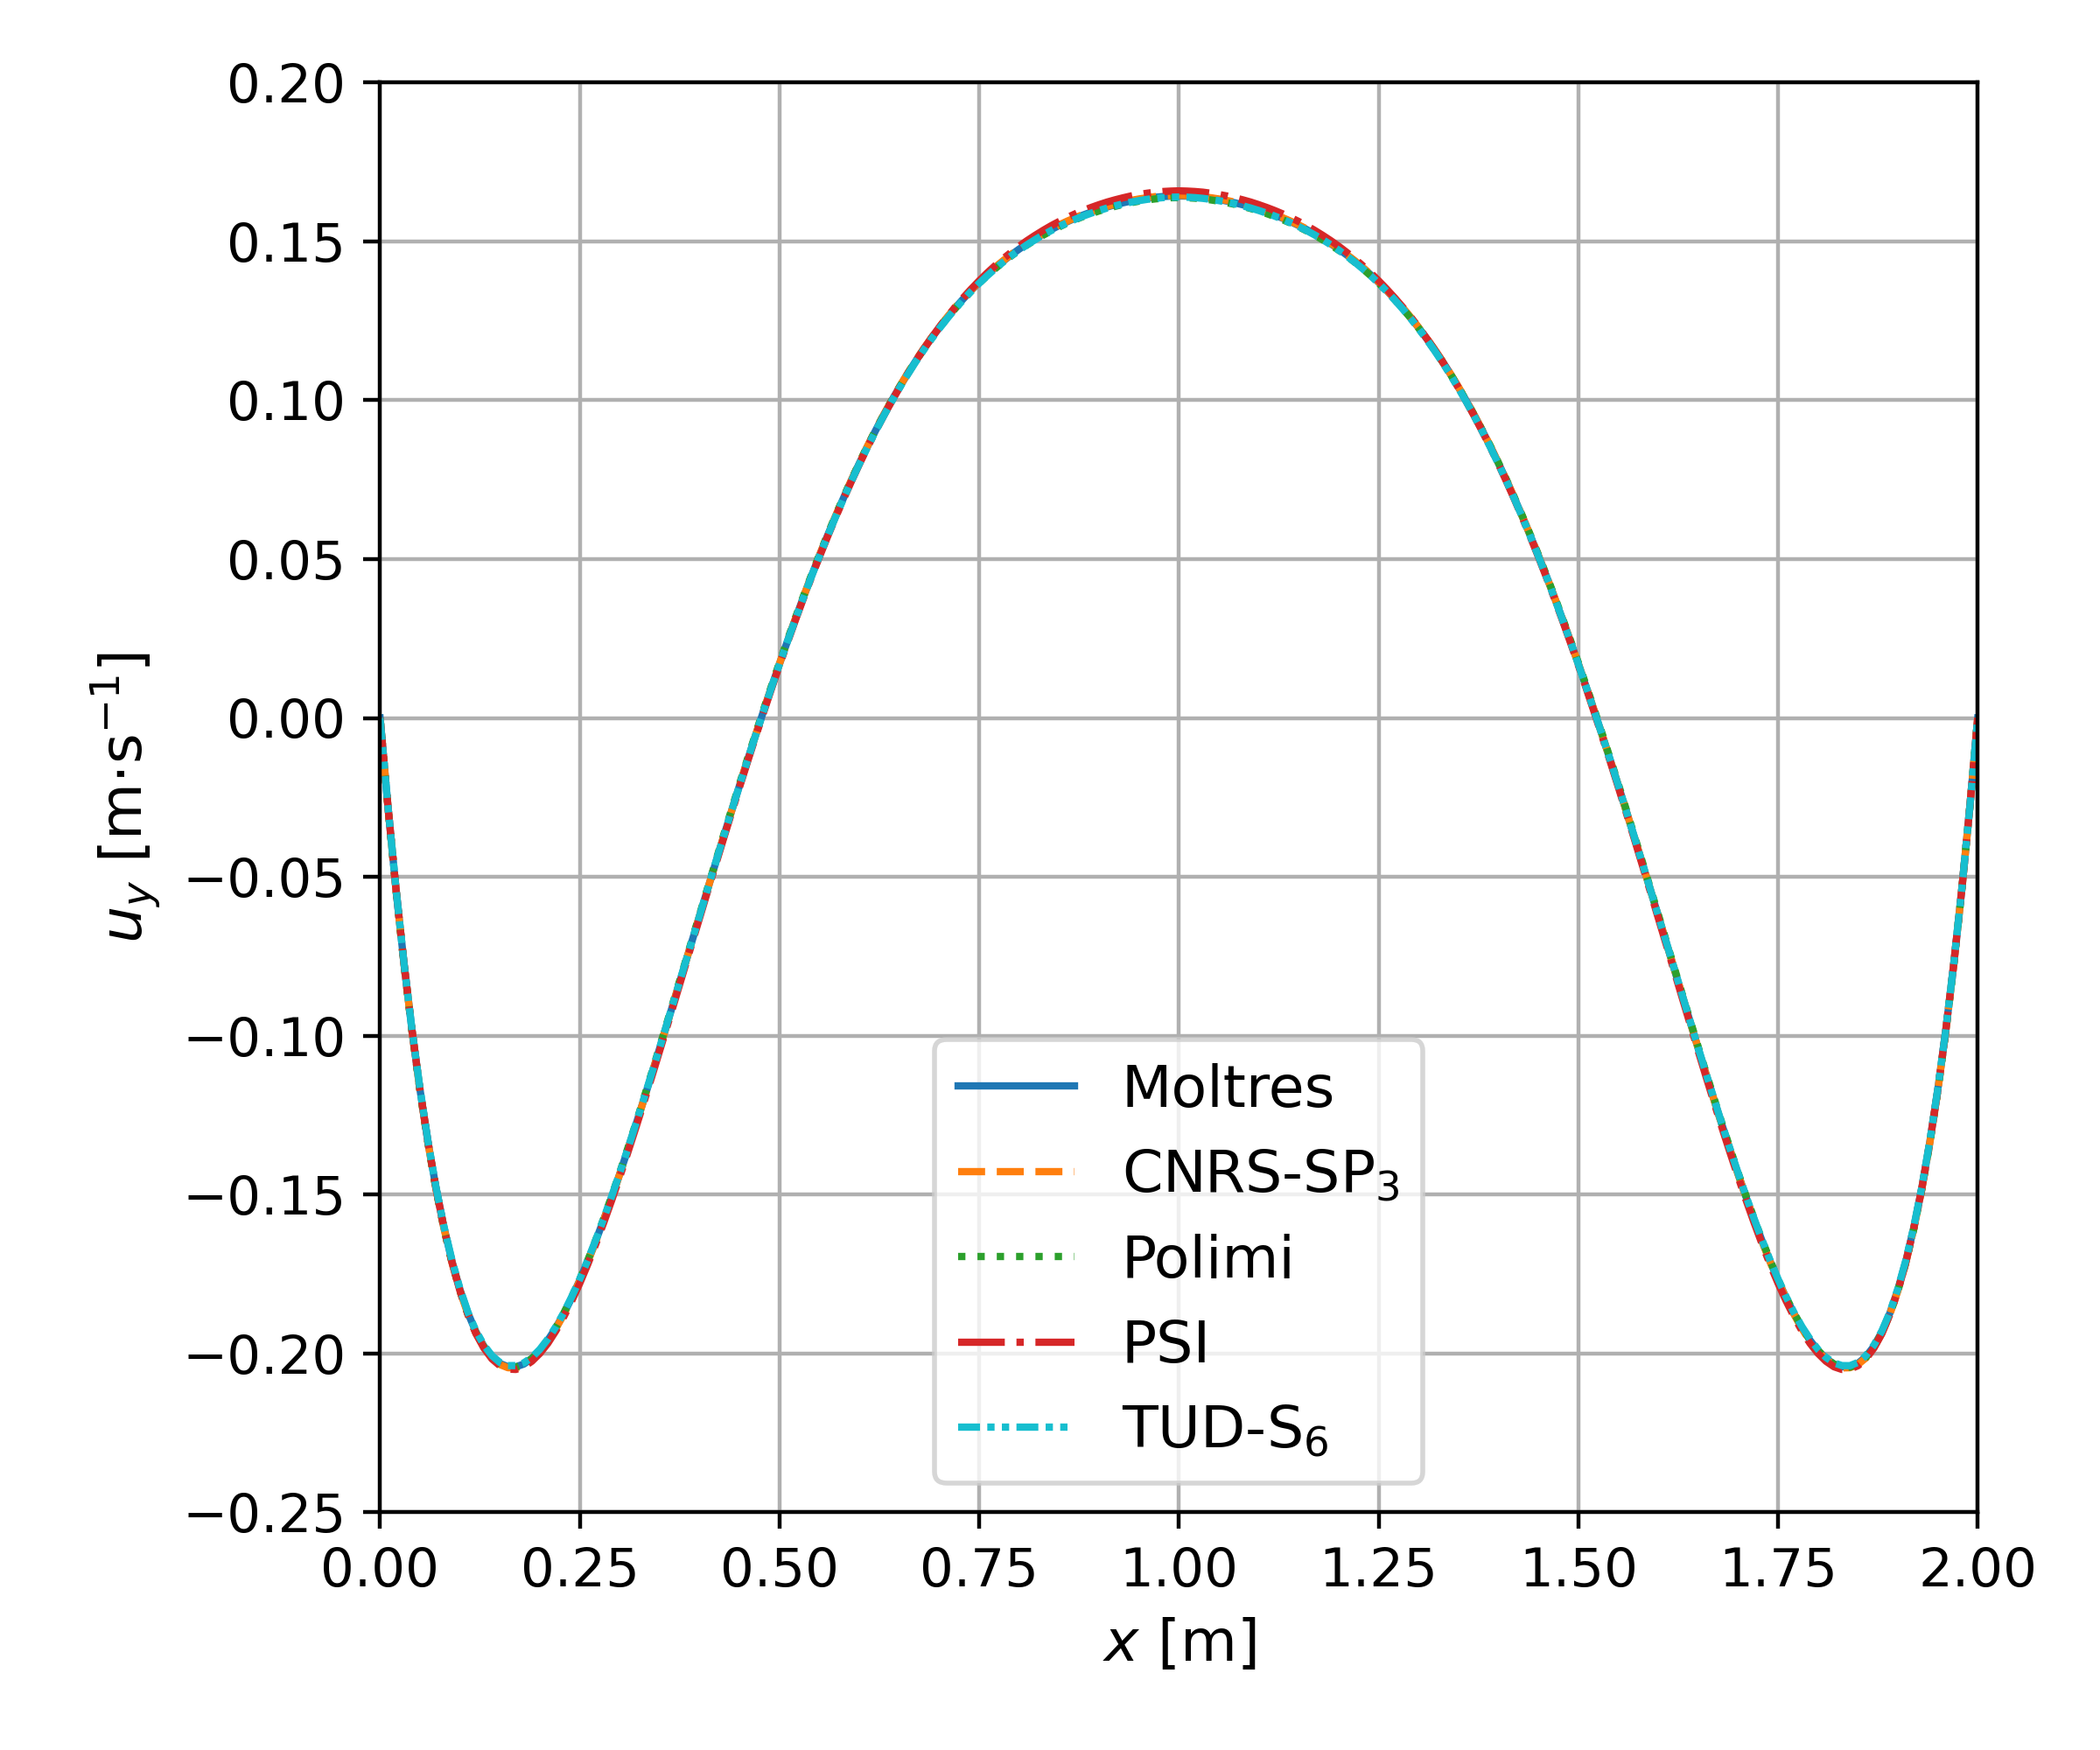
\includegraphics[width=.49\columnwidth]{1-3-vel-plot}
	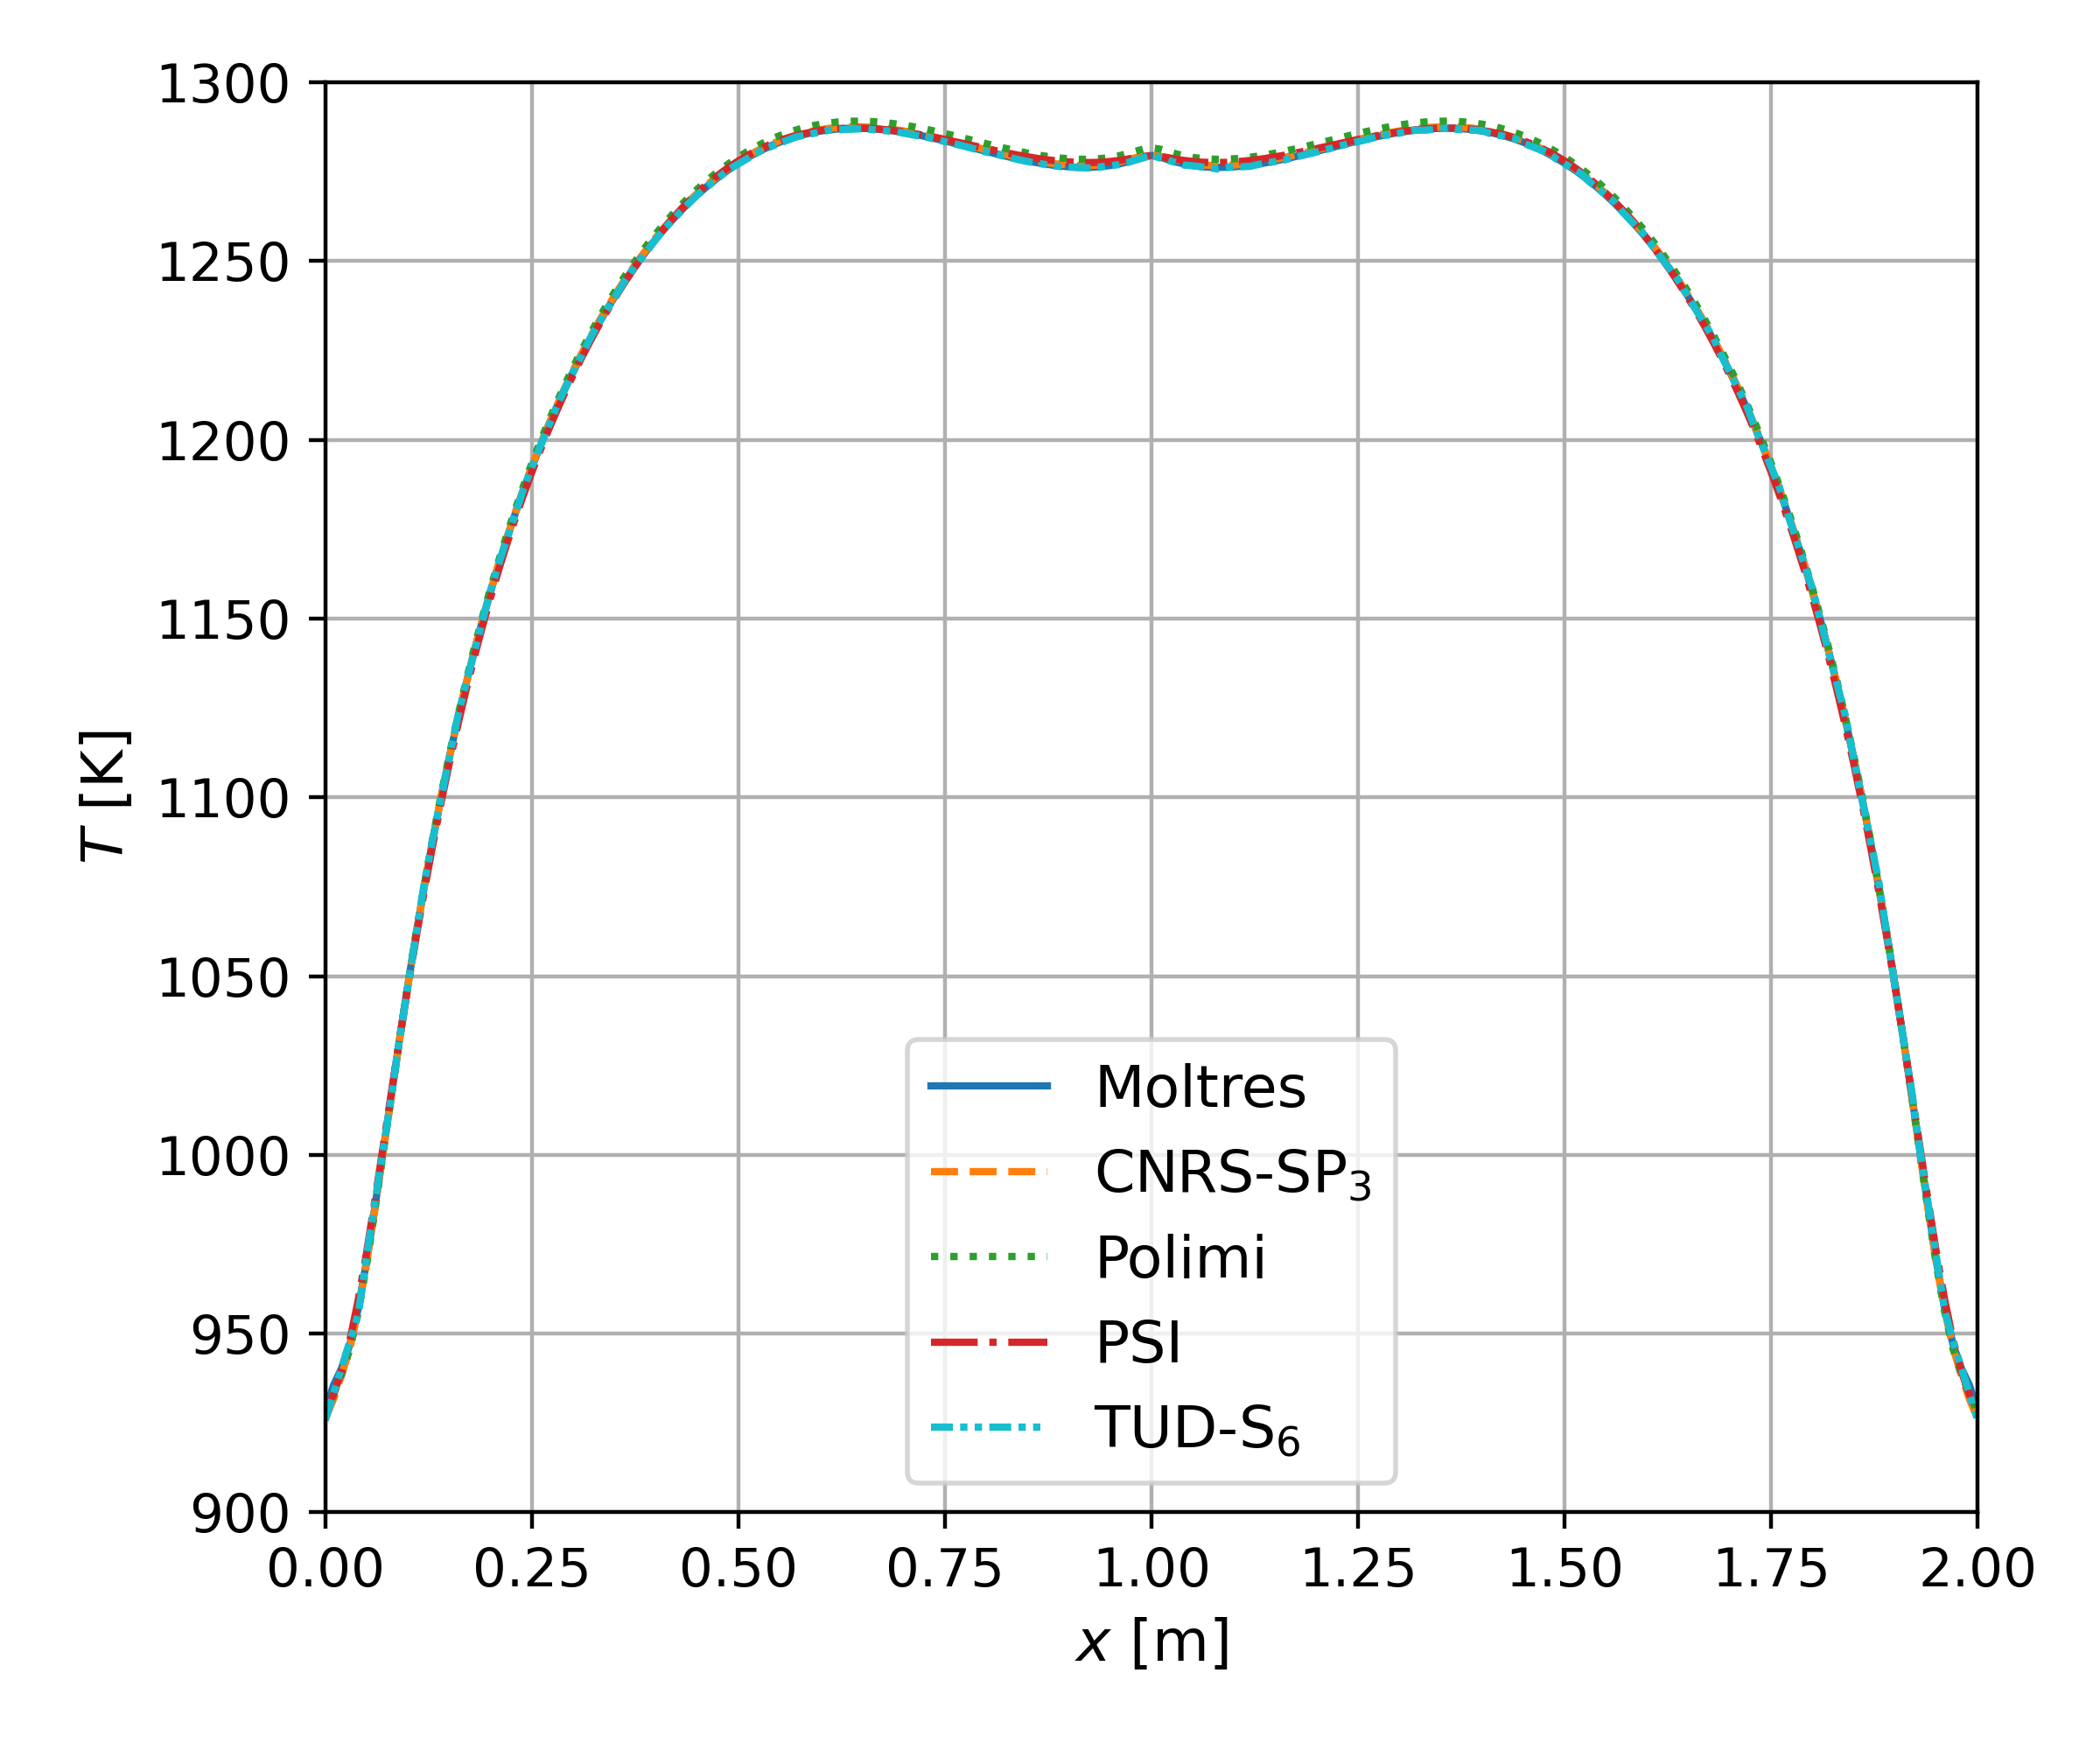
\includegraphics[width=.49\columnwidth]{1-3-temp-plot}
	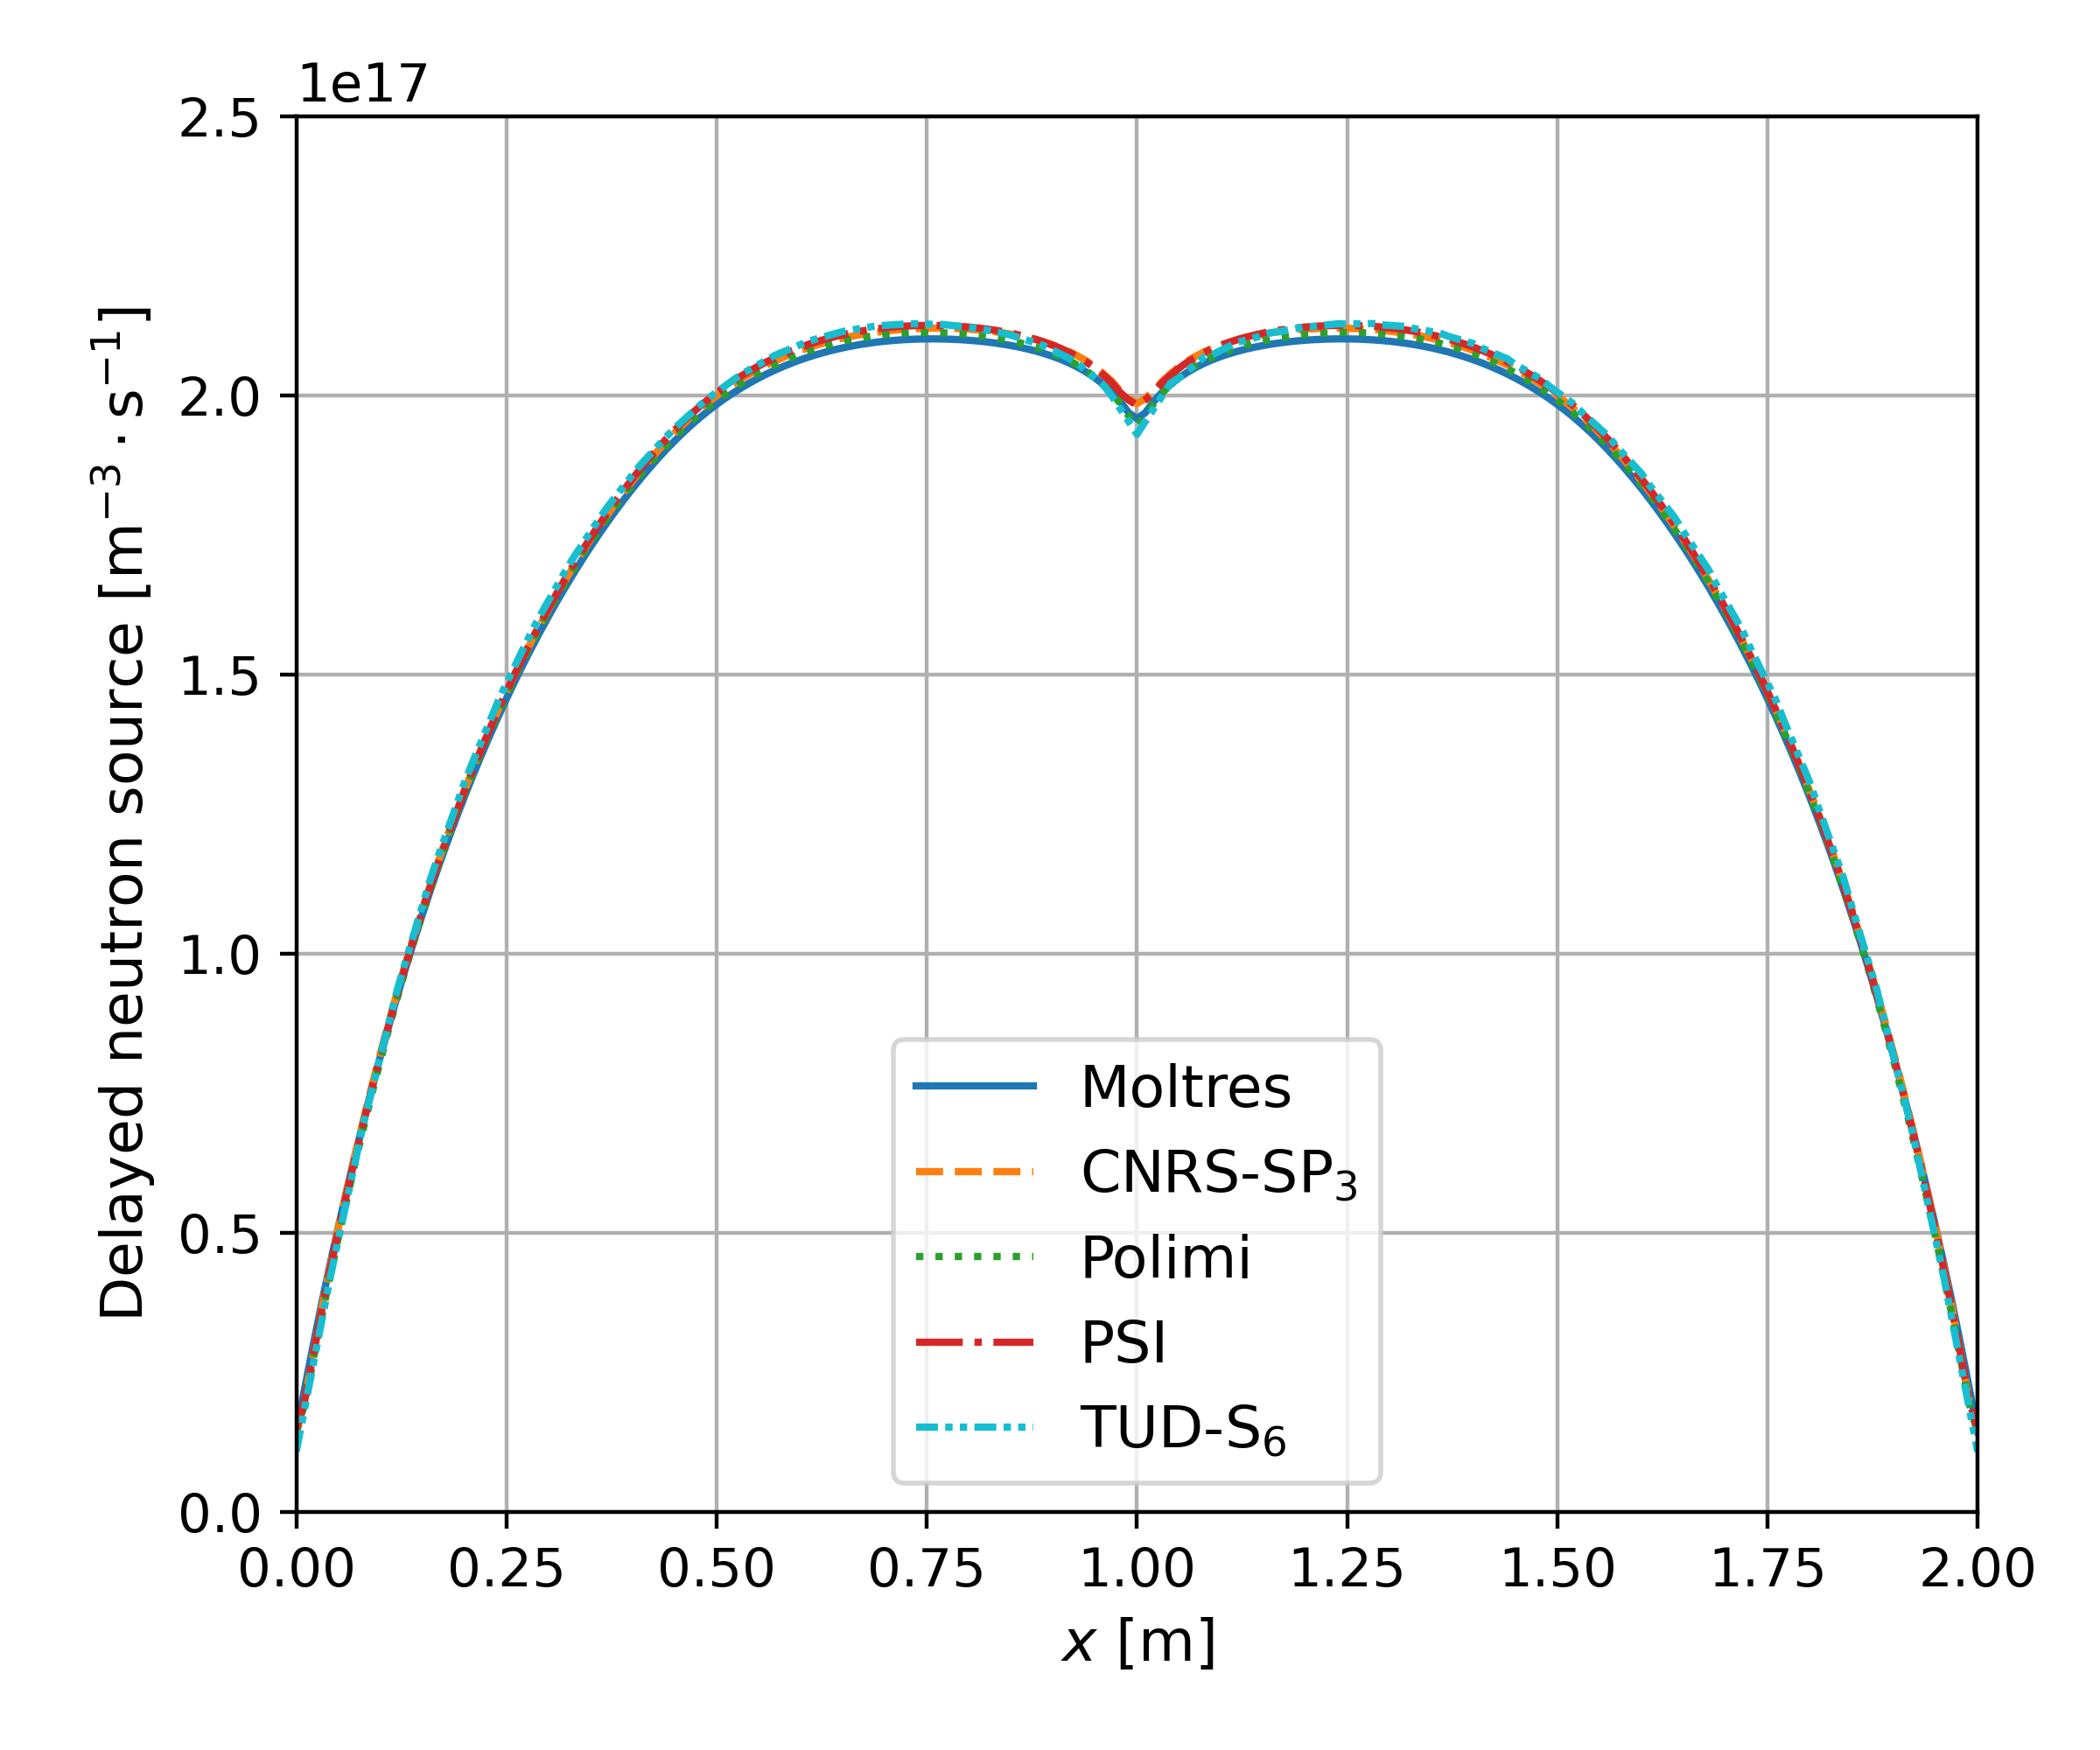
\includegraphics[width=.49\columnwidth]{1-3-dnp-plot}
	\caption{Step 1.3 \textemdash\ Vertical velocity component, temperature distribution,
	and delayed neutron source along AA'.}
	\label{fig:1.3}
\end{figure}

\FloatBarrier

\paragraph{Step 1.4: Full coupling}

Figure \ref{fig:cnrs-color} shows 2D temperature distribution and velocity
streamlines from Moltres for Step 1.4 with $U_{lid} = 0.5$ m$\cdot$s$^{-1}$ and
$P = 1$ GW. Table \ref{table:full} shows the change in $\rho$ under the various
$U_{lid}$ and $P$ values. Refer to Tiberga et al.'s paper
\cite{tiberga_results_2020} for the benchmark participants' corresponding
values. The change in $\rho$ values from Moltres all fall within the range of
benchmark values
for all cases. Furthermore, the $\Delta\rho$ values are all within 1.1 pcm of
the corresponding values from the TUD-S$_2$ model in the benchmark paper. Given
that the $S_2$ discrete ordinates method with isotropic sources is theoretically equivalent to the
multigroup neutron diffusion method, Moltres is largely
consistent with the benchmark participants outside of differences from the
neutronics models.

\begin{figure}[htb]
  \centering
  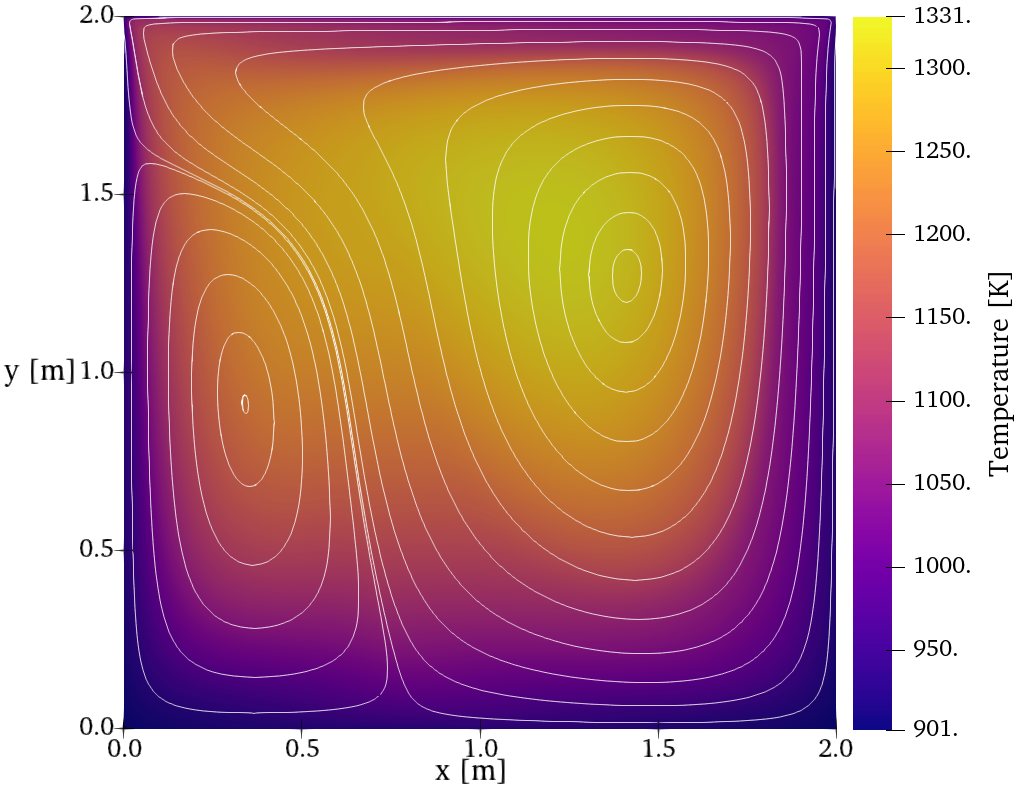
\includegraphics[width=.7\columnwidth]{full-coupled}
  \caption{Temperature distribution from Moltres for the fully coupled
  system (Step 1.4) with buoyancy effects, $P = 1$ GW, and $U_{lid} = 0.5$
  m$\cdot$s$^{-1}$. The lines correspond to the streamlines of the velocity
  field.}
  \label{fig:cnrs-color}
\end{figure}
%
\begin{table}[htb]
	\caption{Reactivity change in Step 1.4, relative to Step 0.2 under various
	$U_{lid}$ and $P$ values.}
	\centering
	\small
	\setlength\tabcolsep{1.5pt}
	\begin{tabular}{c c c c c c}
		\toprule
		& \multicolumn{5}{c}{$\rho_{s1.4} - \rho_{s0.2}$ [pcm]} \\
		\midrule
		{\backslashbox{$U_{lid}$ [m$\cdot$s$^{-1}$]}{$P$ [GW]}} & 0.2 & 0.4 & 0.6 & 0.8 & 1.0 \\
		\midrule
		0.0 & -263.7 & -498.3 & -730.9 & -966.7 & -1207.7 \\
		0.1 & -265.9 & -498.7 & -730.6 & -966.0 & -1206.7 \\
		0.2 & -268.1 & -498.8 & -729.4 & -963.7 & -1203.6 \\
		0.3 & -269.9 & -498.5 & -727.8 & -960.8 & -1199.5 \\
		0.4 & -271.9 & -498.5 & -726.5 & -958.3 & -1195.7 \\
		0.5 & -274.2 & -498.7 & -725.6 & -956.4 & -1192.7 \\
		\bottomrule
	\end{tabular}
	\label{table:full}
\end{table}

\FloatBarrier

\begin{table}[htb]
	\caption{Discrepancy values from Moltres alongside the average and standard
	deviation of the discrepancy values of the benchmark participants for Step
	2.1.}
	\centering
	\small
	\begin{tabular}{l l S S S}
		\toprule
		\multirow{2}{*}{\textbf{Step}} & \multirow{2}{*}{\textbf{Observable}} & {\multirow{2}{*}{\textbf{Moltres [\%]}}} & \multicolumn{2}{c}{\textbf{Benchmark [\%]}} \\
		& & & {Average} & {SD} \\
		\midrule
		\multirow{2}{*}{2.1} & Gain & 0.493 & 0.587 & 0.244 \\
		\cmidrule{2-5}
		& Phase shift & 1.741 & 2.176 & 0.554 \\
		\bottomrule
	\end{tabular}
	\label{table:disc2}
\end{table}
%
\begin{figure}[htb]
	\centering
	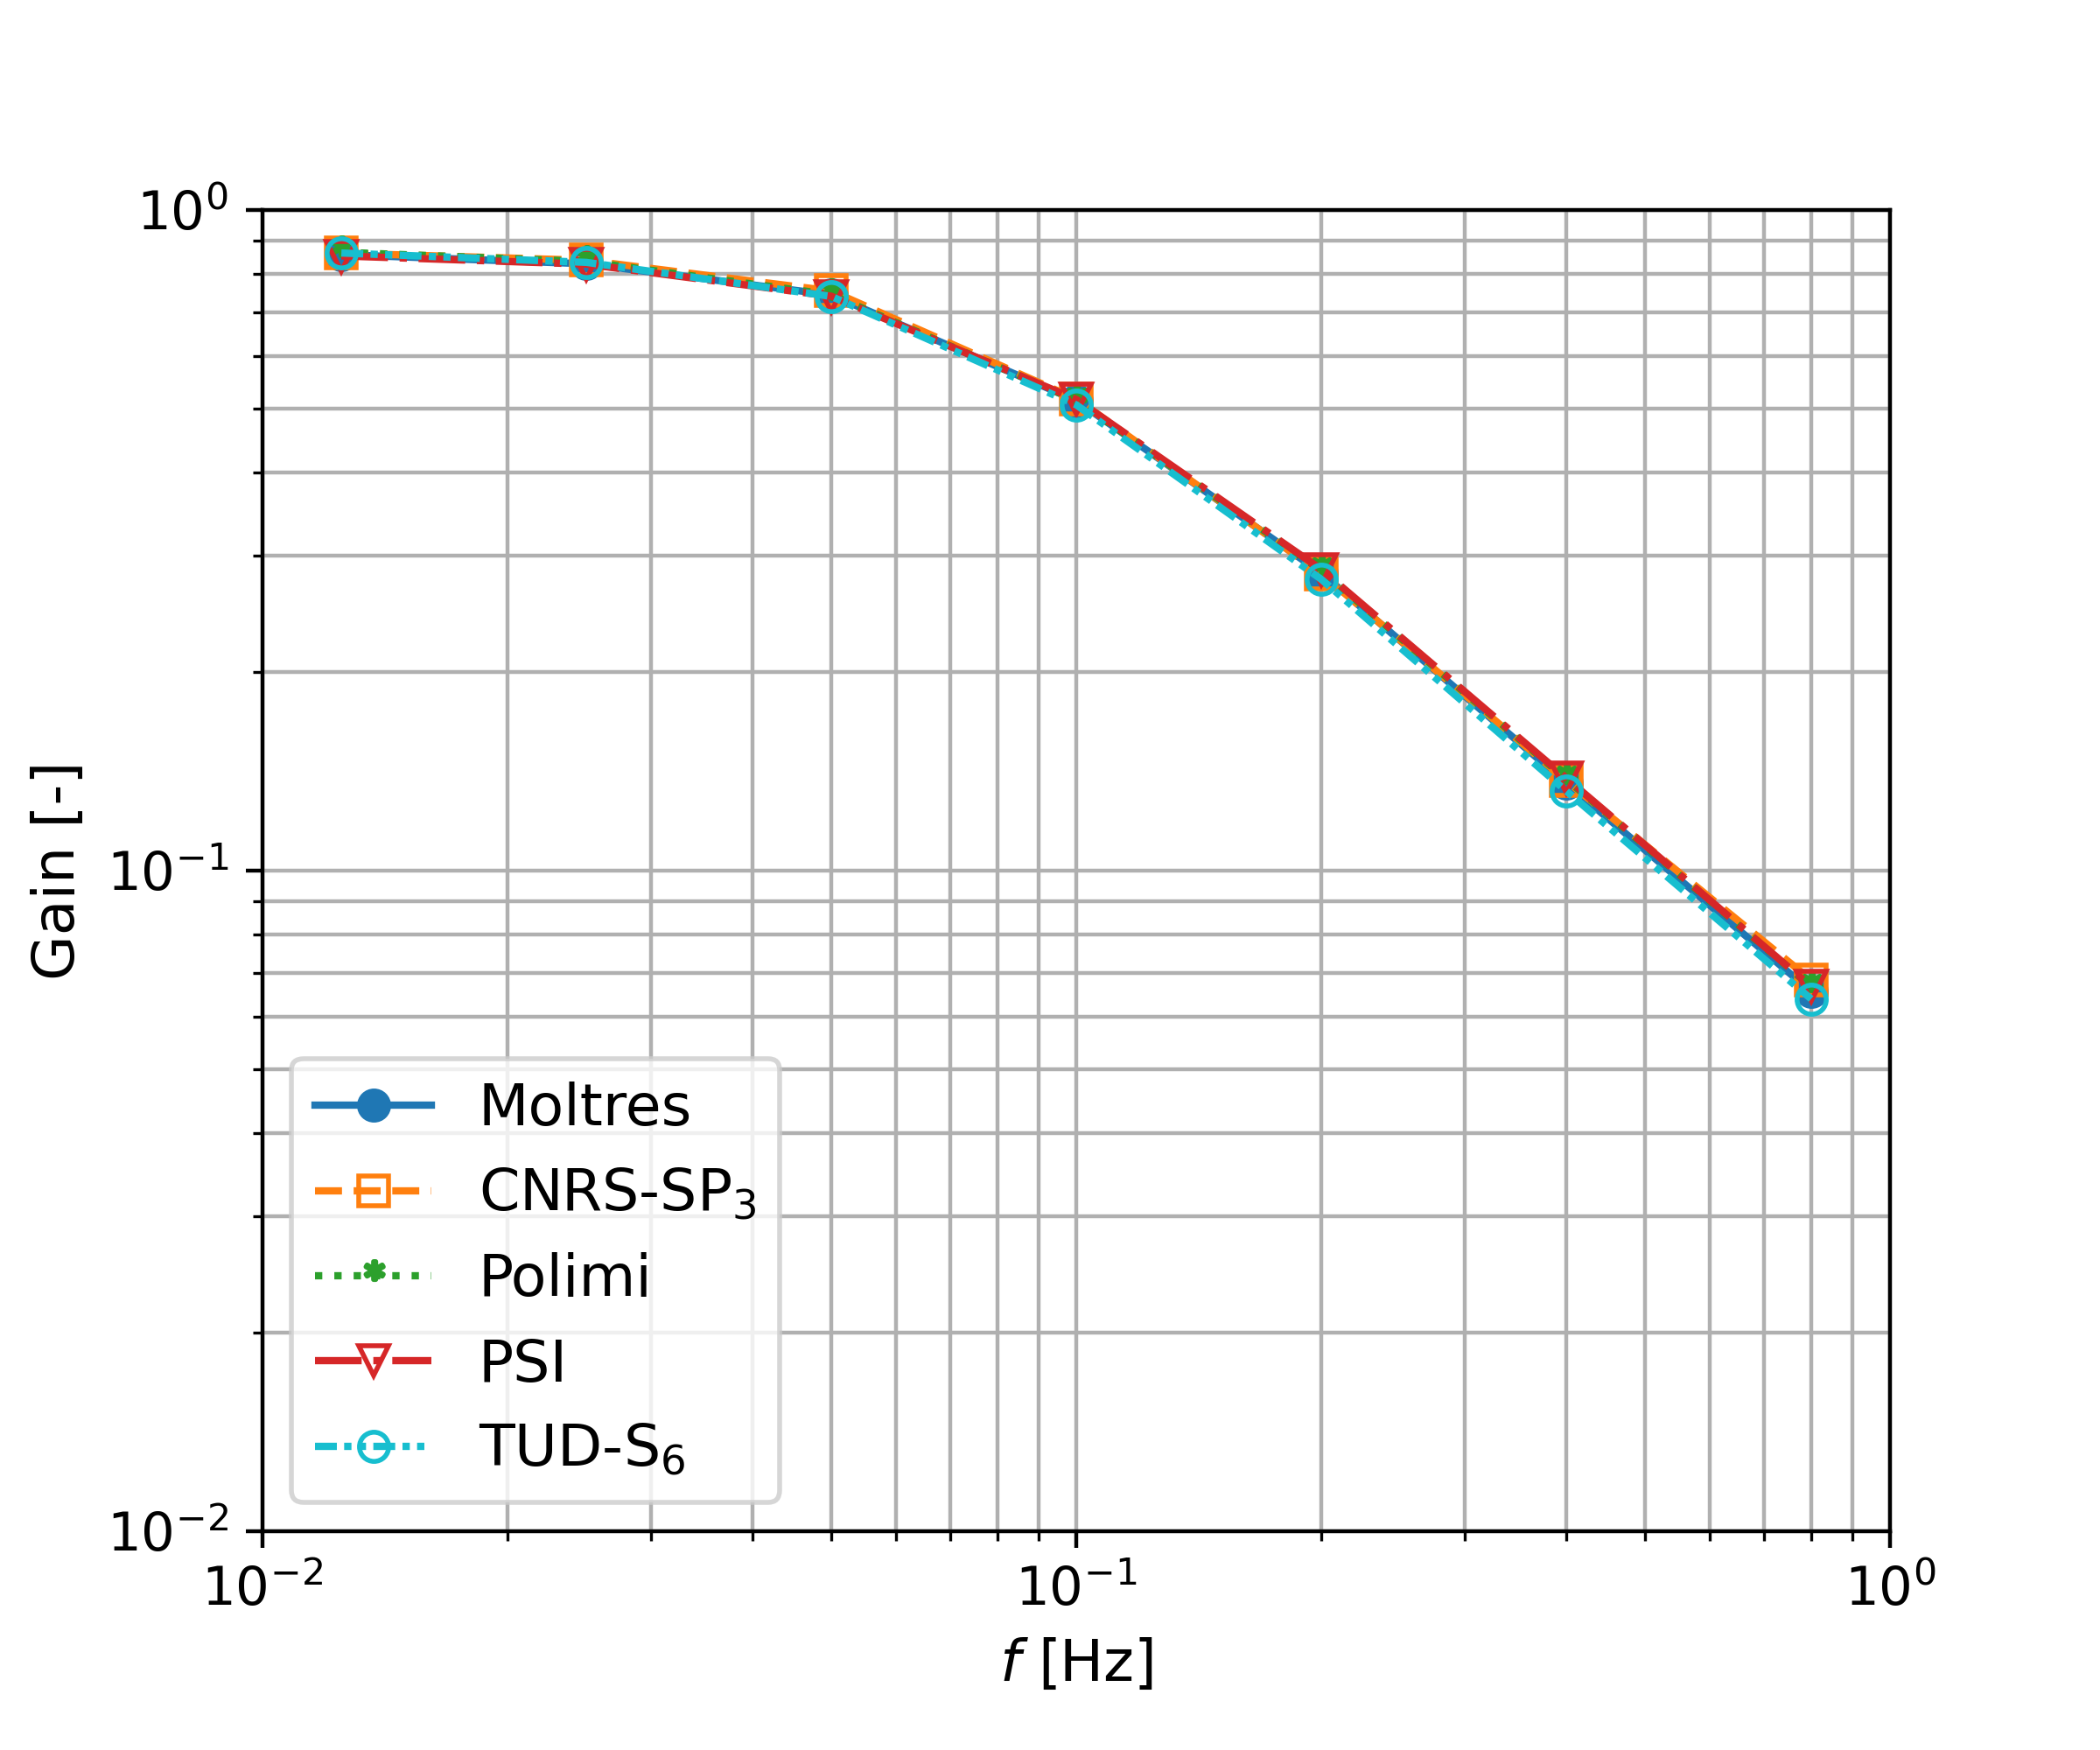
\includegraphics[width=.49\columnwidth]{2-1-gain-plot}
	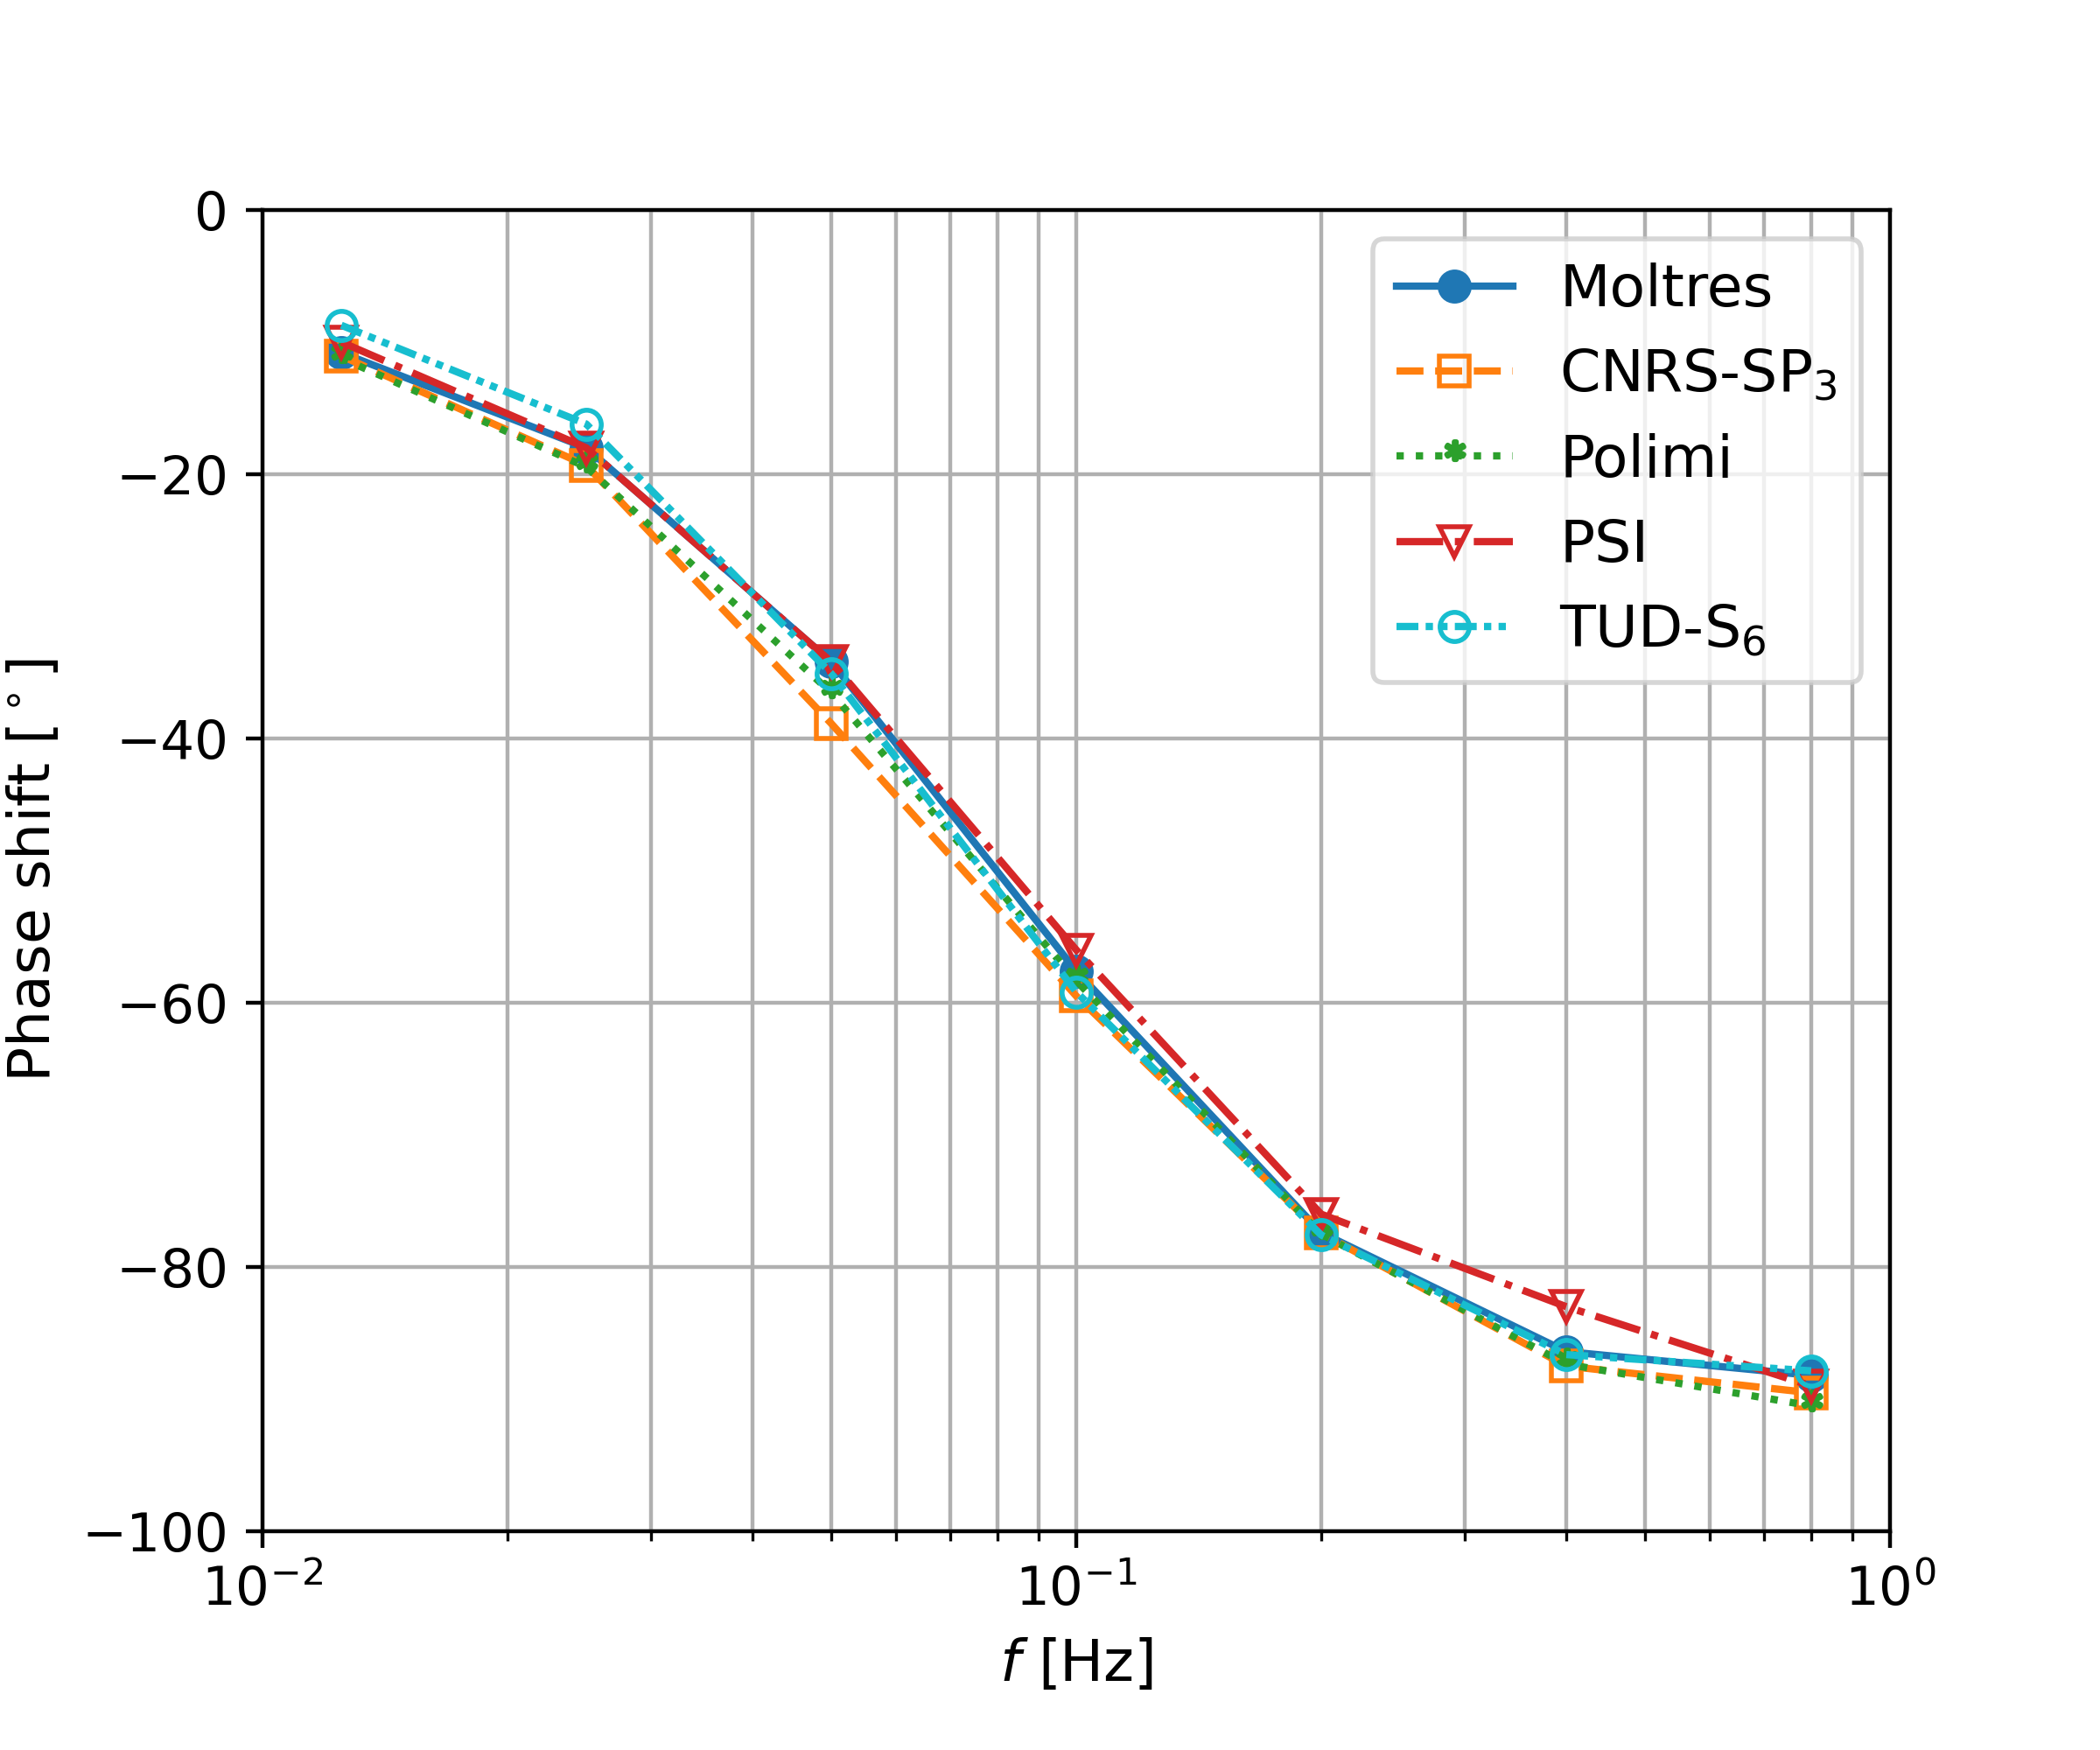
\includegraphics[width=.49\columnwidth]{2-1-phase-plot}
	\caption{Step 2.1 \textemdash\ Bode gain and phase plots of the frequency response of
	the fully coupled system.}
	\label{fig:2.1}
\end{figure}

\subsubsection{Phase 2 results \& discussion}

Lastly, the following subsection discusses the results for the transient cases
in Step 2.1, which involve measuring the response in power output to periodic
perturbations in the heat transfer coefficient.

\paragraph{Step 2.1: Forced convection transient}

Figure \ref{fig:2.1} shows the Bode gain and phase shift plots of the response
in power output in the fully coupled system. Along with the average discrepancy
values from Table \ref{table:disc2}, the results show that Moltres is
consistent with the benchmark. The gain data points from all \gls{MSR} software
agree closely with one another. Moltres reports an average discrepancy value of
0.496\%, slightly lower than the benchmark average of 0.587\%. On the other
hand, the phase shift data points show a greater spread over the various driving
frequencies. We note the different timestepping schemes and timestep
sizes among the different software packages, which is likely responsible for
the variations in the phase shift. Even with a precision of
$\pm0.9^\circ$ for each phase shift value, Moltres accurately reproduces the
correct trend with a lower average discrepancy (1.741\%) than the benchmark
participants' average (2.176\%).

\FloatBarrier

\subsection{Summary}

\glspl{MSR} feature significant multiphysics interactions, presenting
computational challenges for many existing multiphysics reactor analysis
software. This chapter presents code-to-code verification of Moltres'
capabilities in modeling such multiphysics phenomena in fast-spectrum
\glspl{MSR} based on the CNRS benchmark \cite{tiberga_results_2020}.
The CNRS benchmark assesses multiphysics \gls{MSR} simulation
software through several steps involving single-physics and coupled
neutronics/thermal-hydraulics problems.

The results showed that Moltres is consistent with the participating software
presented in the CNRS benchmark paper for modeling important phenomena
in fast-spectrum \glspl{MSR}. The percentage discrepancies in the various
neutronics, velocity, and temperature quantities mostly fall below or within
one standard deviation of the average of the benchmark participants.
Minor deviations in the temperature in Steps 0.3 and 1.2 
stem from the discontinuous velocity
boundaries on the top corners in the lid-driven cavity flow. We have shown that
these deviations are limited to the top boundary of the domain and do not
affect the rest of the physical parameters. The results from
Moltres agree closest with the TUD-S$_2$ software package, which implements the
$S_2$ discrete ordinates method for
neutron transport on a uniform structured mesh with a \gls{DFEM}-based solver.
These features make Moltres the most similar to the TUD-$S_2$ model as compared
to the other models, which employ different neutron transport models,
non-uniform meshes, or finite volume-based solvers.

This work verifies Moltres' capabilities for future work involving the modeling and
simulation of fast-spectrum \glspl{MSR} such as the European \gls{MSFR} and
TerraPower's \gls{MCFR} \cite{terrapower_terrapower_2021}. Notably, the CNRS
benchmark does not assess modeling capabilities for complex physics phenomena
such as turbulent flow in \glspl{MSR}. However, we expect coolant loops in many \gls{MSR} designs
will experience turbulent flow under regular operation or accident scenarios.
These expectations, alongside the subpar results of pump-initiated accidents
reported in Section \ref{sec:msfr}, call for the implementation and
verification of a turbulence model in Moltres to accurately model \glspl{MSR}.

\FloatBarrier



\section{MSRE Zero-Power Pump Experiments}

\section{Spalart-Allmaras Turbulence Model Verification}

\section{Moltres Spalart-Allmaras Turbulence Model Verification} \label{sec:turbulence}

As detailed in Section \ref{sec:th}, Moltres compiles with the MOOSE Navier-Stokes
\cite{peterson_overview_2018} and Heat Transfer modules for incompressible flow
modeling capabilities by default. Moltres couples with these modules natively because they are all
built on the MOOSE framework.

To address the lack of turbulence modeling in Moltres, I implemented a Spalart-Allmaras turbulence model
\cite{spalart_one-equation_1994}, described in Section \ref{sec:lit-turb}, with \gls{SUPG}
stabilization on Moltres. The Spalart-Allmaras model estimates the turbulent eddy viscosity defined by the
eddy viscosity hypothesis applied to the \gls{RANS} equations \cite{rodi_turbulence_2017}.
On balance the Spalart-Allmaras model is a complete (does not require prior
knowledge of the actual turbulence behavior) and computationally efficient one-equation turbulence
model for approximating wall-bounded turbulent flows. The Spalart-Allmaras model implementation in Moltres
couples seamlessly with the continuous \gls{FEM} \gls{INSAD}
\cite{peterson_overview_2018, lindsay_automatic_2021} model
from the Navier-Stokes module. Alongside the Spalart-Allmaras model, Moltres also now has turbulent
diffusion physics kernels for temperature and the delayed neutron precursors.

The SA model in Moltres follows the Spalart-Allmaras model with a rotation correction scheme
\cite{aupoix_extensions_2003, dacles-mariani_numericalexperimental_1995} as described on the
\gls{NASA} Turbulence Modeling Resource website \cite{rumsey_turbulence_nodate}. The rotation
correction reduces eddy viscosity in regions of rotational but non-turbulent flow where the
original Spalart-Allmaras model overestimates eddy viscosity. The Spalart-Allmaras model implementation in Moltres
solves for the modified dynamic viscosity $\tilde{\mu}$ (as opposed to $\tilde{\nu}$) as follows:

\begin{gather}
  \rho \frac{\partial\tilde{\mu}}{\partial t} + \rho \mathbf{u}\cdot\nabla\tilde{\mu} = \rho c_{b1}
  \left(1-f_{t2}\right)\tilde{S}\tilde{\mu} + \frac{1}{\sigma}\{\nabla\cdot\left[\left(\mu+
  \tilde{\mu}\right)\nabla\tilde{\mu}\right] + c_{b2}|\nabla\tilde{\mu}|^2\} - \left(c_{w1}f_w -
  \frac{c_{b1}}{\kappa^2}f_{t2}\right)\left(
  \frac{\tilde{\mu}}{d}\right)^2
  \shortintertext{where}
  \begin{align*}
    \mu_t &= \tilde{\mu}f_{v1} = \text{turbulent eddy viscosity}, \\
    f_{v1} &= \frac{\chi^3}{\chi^3 + c_{v1}^3}, \\
    \chi &= \frac{\tilde{\mu}}{\mu}, \\
    \tilde{S} &= \Omega + \frac{\tilde{\nu}}{\kappa^2 d^2} f_{v2}, \\
    f_{v2} &= 1 - \frac{\chi}{1+\chi f_{v1}}, \\
    \Omega &= \sqrt{2W_{ij}W_{ij}} = \text{vorticity magnitude}, \\
    W_{ij} &= \frac{1}{2}\left(\frac{\partial u_i}{\partial x_j} - \frac{\partial u_j}{\partial x_i}
    \right), \\
      f_w &= g\left(\frac{1 + c_{w3}^6}{g^6 + c_{w3}^6}\right)^{1/6}, \\
      g &= r + c_{w2}\left(r^6 - r\right), \\
      r &= \text{min}\left(\frac{\tilde{\nu}}{\tilde{S}\kappa^2d^2}, 10\right), \\
      f_{t2} &= c_{t3} \exp{\left(-c_{t4}\chi^2\right)},
  \end{align*}
\shortintertext{and the constants are}
  \sigma = \frac{2}{3}, \ c_{b1} = 0.1355, \ c_{b2} = 0.622, \ \kappa = 0.41, \
  c_{w1} = \frac{c_{b1}}{\kappa^2} + \frac{1+c_{b2}}{\sigma}, \nonumber \\
  c_{w2} = 0.3, \ c_{w3} = 2, \
  c_{v1} = 7.1, \ c_{t3} = 1.2, \ c_{t4} = 0.5 \ \text{.} \nonumber
\end{gather}

The $f_{t2}$ turbulence trip term is togglable using the \texttt{use\_ft2\_term} input parameter
(false by default) if turbulence trip (initiation) is not necessary
\cite{rumsey_turbulence_nodate}. The following subsections cover verification and validation tests
of the Spalart-Allmaras model in Moltres using reference problems for turbulent channel, pipe, and
\gls{BFS} flow. Moltres input files
for all three reference problems are available at
\url{https://github.com/arfc/moltres/tree/devel/problems/2023-basic-turbulence-cases}.
The Moltres test dataset is available on Zenodo at this reference listing \cite{park_dataset_2023}.

\subsection{Turbulent Channel Flow Verification Test}

Moser et al.\ \cite{moser_direct_1999} performed \gls{DNS} simulations of turbulent channel flow
for friction Reynolds number, Re$_\tau\approx395$ (corresponds to Reynolds number, Re
$\approx 13750$). Their results serve as the reference solution for this turbulent channel flow
test.

The Moltres model for this test is a 2-D 140 m$\times$0.5 m half-channel
(Figure \ref{fig:channel-geom}). The main flow direction
is in the positive $x$ direction with the inlet and outlet on the left and right ends,
respectively. The channel wall lies along the top boundary ($y=0.5$ m) while the bottom boundary
($y=0$ m) serves as a symmetry axis for the half-channel geometry. Figure \ref{fig:channel-mesh}
shows a close-up view of the refined mesh near the inlet and along the top wall boundary. The mesh
for the rest of the channel geometry follows the same mesh resolution as the rightmost column of
elements shown on the right side of Figure \ref{fig:channel-mesh}. The dimensionless wall distance
parameter $y^+$ of the first mesh element along wall boundary for fully developed flow at the end
of the channel is 0.974, meeting the
$y^+ \lesssim 1$ requirement for properly wall-resolved flow. Table \ref{table:channel} lists
relevant flow parameters for the turbulent channel flow test. The Moltres channel flow model
ran as a time-dependent simulation with adaptive time-stepping starting from a timestep size of 0.1
s up to a maximum timestep size of 10 s with a timestep size growth factor of 1.1. The simulation
automatically terminated at $t=186$ s when Moltres detected that the flow profile reached
steady-state, i.e., the flow and turbulent viscosity distributions remained unchanged between
successive timesteps.

\begin{figure}[p]
  \centering
  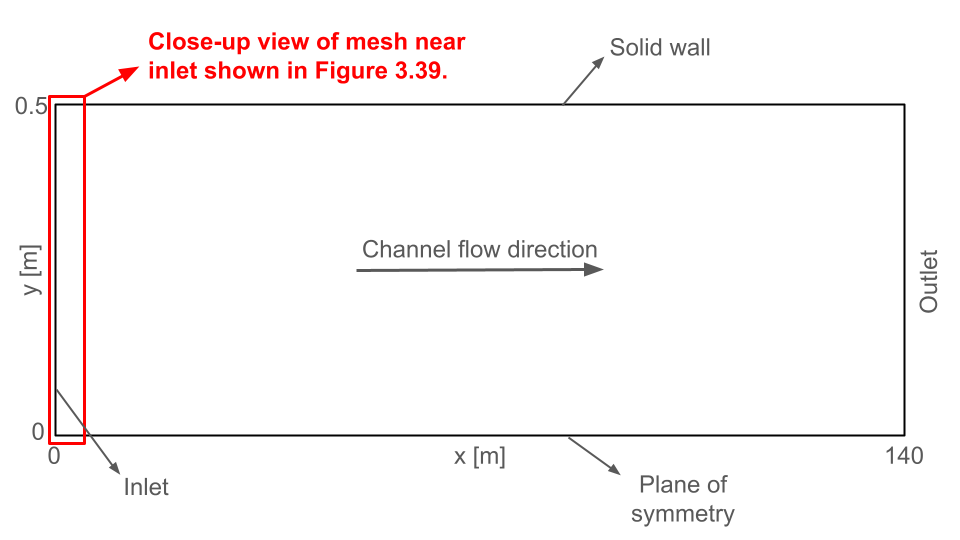
\includegraphics[width=0.9\columnwidth]{channel-geom}
  \caption{Channel geometry for the turbulent channel flow verification test. The red box indicates
  the region shown by the close-up view in Figure \ref{fig:channel-mesh}.}
  \label{fig:channel-geom}
%\end{figure}
%%
%\begin{figure}[htb!]
  \centering
  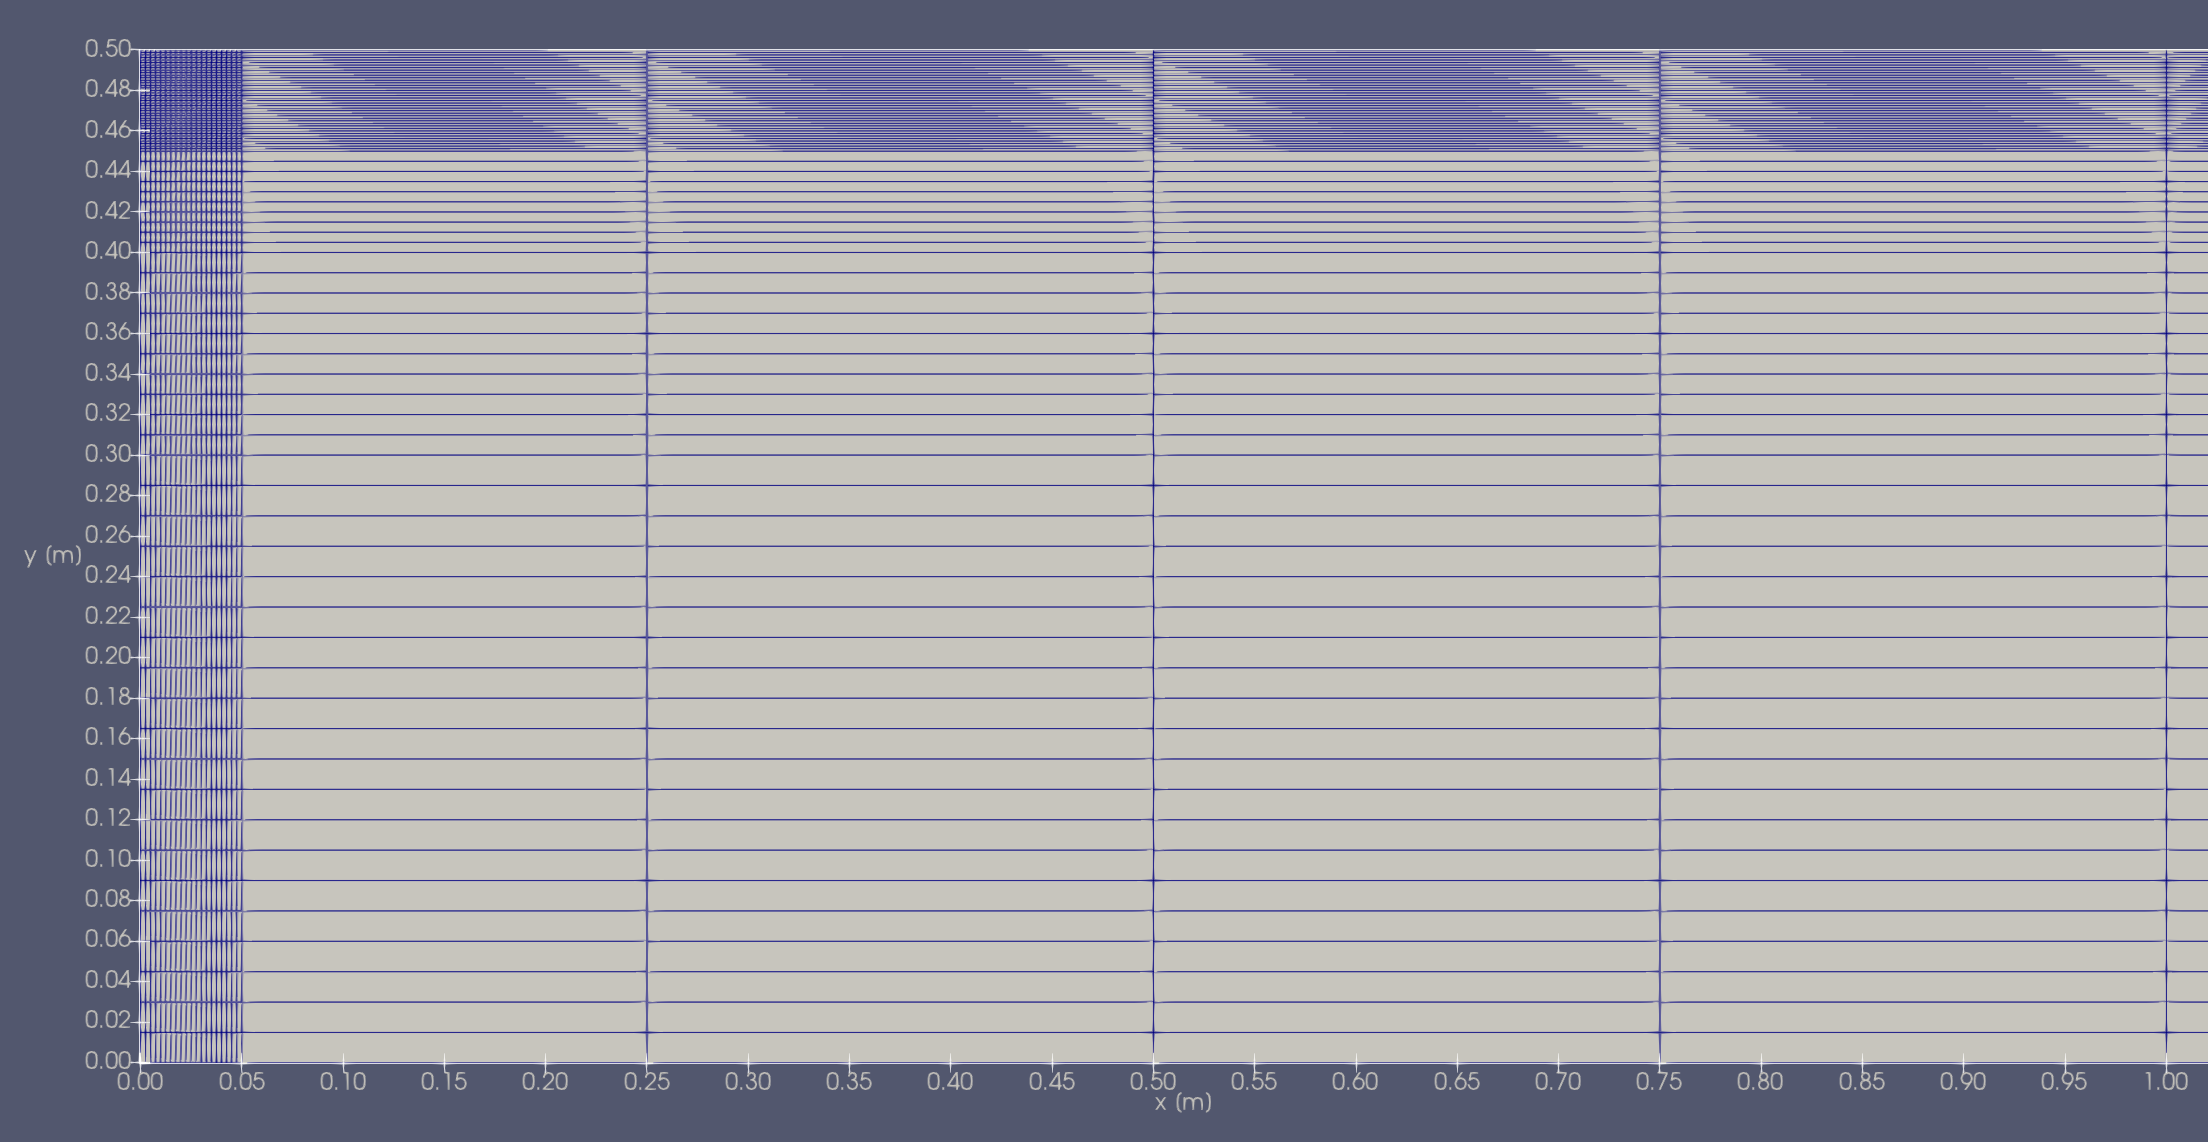
\includegraphics[width=\columnwidth]{channel_mesh}
  \caption{Close-up view of the refined mesh near the inlet (left boundary) for the channel flow
    test. The mesh for the rest of the channel follows the mesh resolution of the rightmost column
  of elements.}
  \label{fig:channel-mesh}
\end{figure}

\begin{table}[htb]
  \centering
  \small
  \caption{Relevant turbulent channel flow problem parameters. The $\tilde{\mu}_\text{inlet}$ value
  at the inlet is set to fives times the $\mu$ value as recommended for the Spalart-Allmaras model
  \cite{spalart_one-equation_1994}.}
  \begin{tabular}{l S}
    \toprule
    Property & {Value} \\
    \midrule
    Density, $\rho$ [kg m$^{-3}$] & 1.0 \\
    Inlet velocity, $v_x$ [m s$^{-1}$] & 1.0 \\
    Dynamic viscosity, $\mu$ [kg m$^{-1}$ s$^{-1}$] & 7.272e-5 \\
    Reynolds number, Re [-] & 1.375e4 \\
    Modified viscosity along inlet, $\tilde{\mu}_\text{inlet}$ [kg m$^{-1}$ s$^{-1}$] & 3.636e-4 \\
    Modified viscosity along wall, $\tilde{\mu}_\text{wall}$ [kg m$^{-1}$ s$^{-1}$] & 0.0 \\
    \bottomrule
  \end{tabular}
  \label{table:channel}
\end{table}

Figure \ref{fig:channel-verification} shows plots of normalized and nondimensionalized velocities,
wall distances, and stresses from the \gls{DNS} data \cite{moser_direct_1999}
and the Moltres Spalart-Allmaras model. The Moltres Spalart-Allmaras model is largely consistent with the reference
\gls{DNS} flow data and reproduces the expected trends in the velocity and stress distributions
across the channel and as a function of the wall distance.

\begin{figure}[htb!]
  \centering
  \begin{subfigure}[b]{0.48\columnwidth}
    \centering
    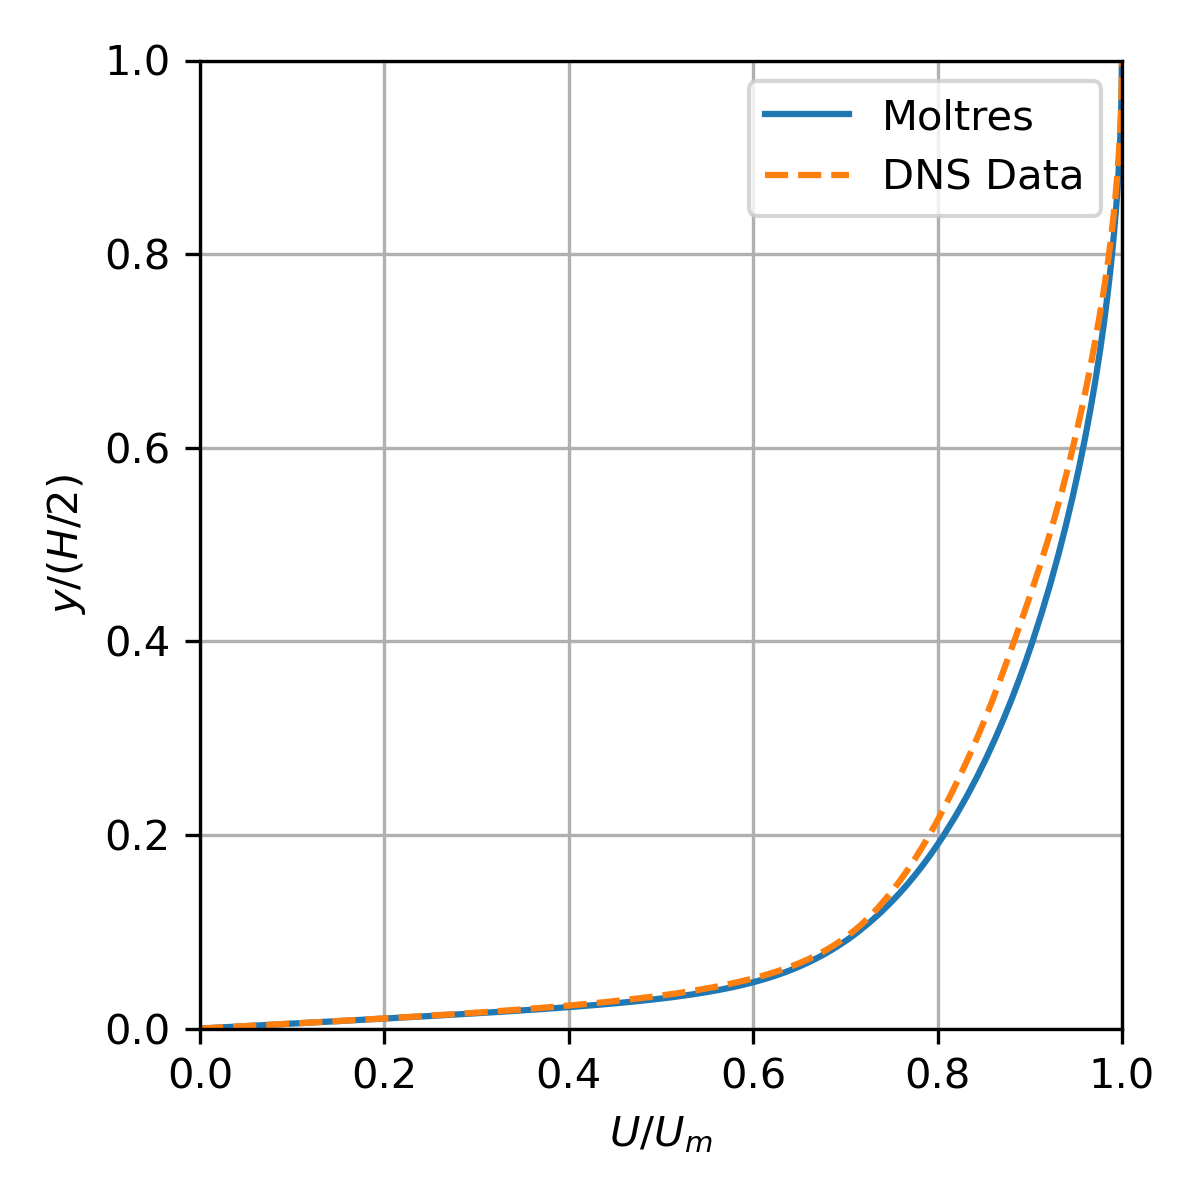
\includegraphics[width=\columnwidth]{channel_vel}
    \caption{Normalized velocity distribution across the channel.}
    \label{fig:channel-vel}
  \end{subfigure}
  \hfill
  \begin{subfigure}[b]{0.48\columnwidth}
    \centering
    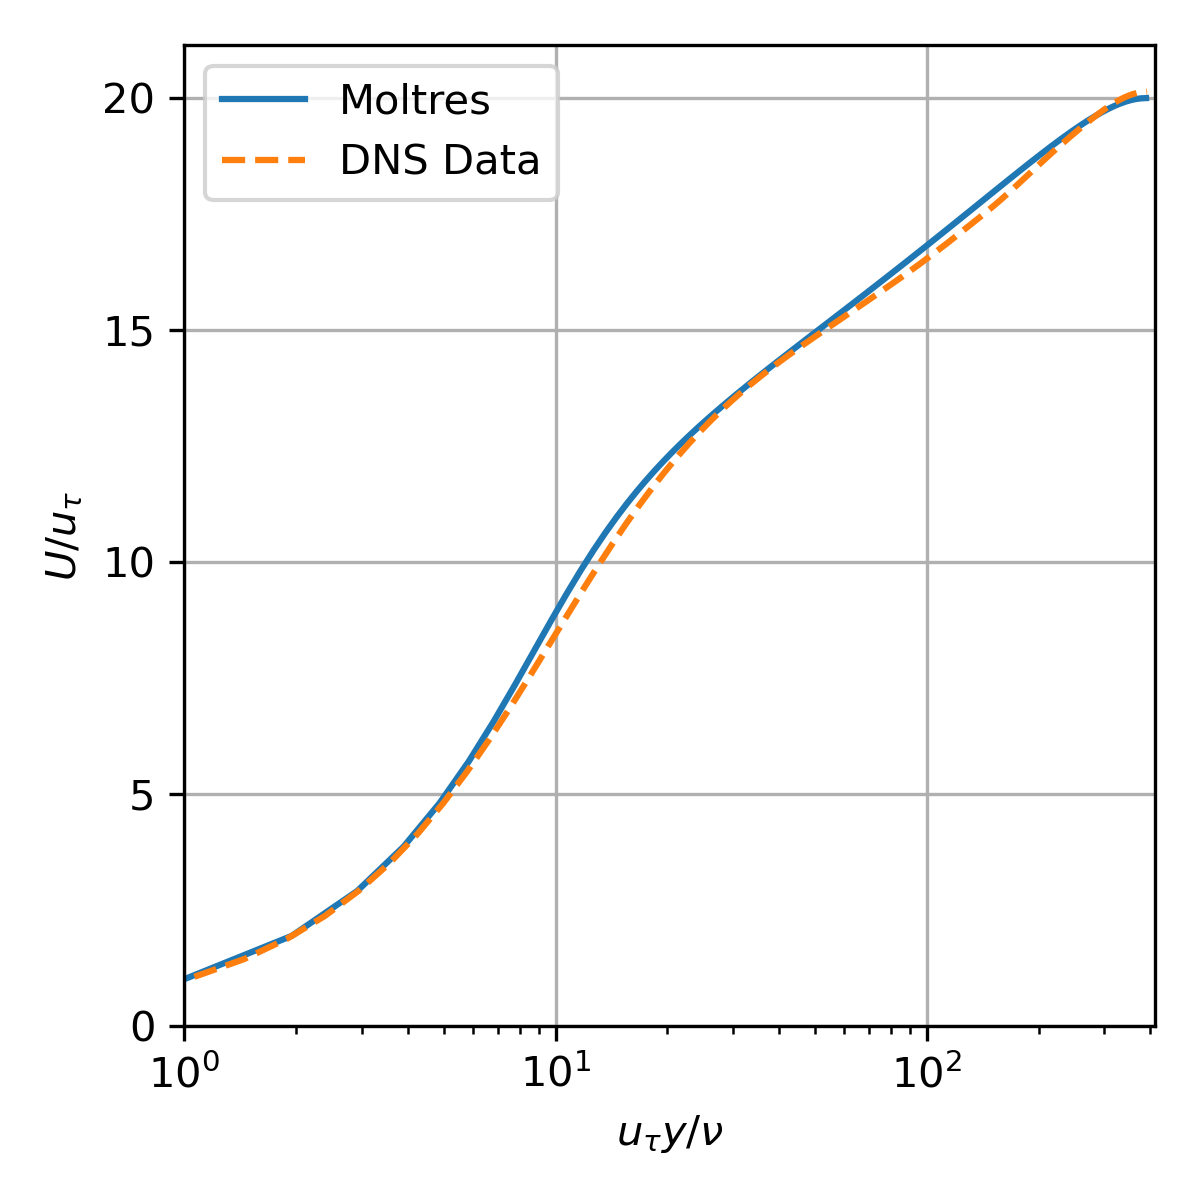
\includegraphics[width=\columnwidth]{channel_nondim}
    \caption{Dimensionless velocity vs.\ dimensionless wall distance.}
    \label{fig:channel-nondim}
  \end{subfigure}
  \begin{subfigure}[b]{0.48\columnwidth}
    \centering
    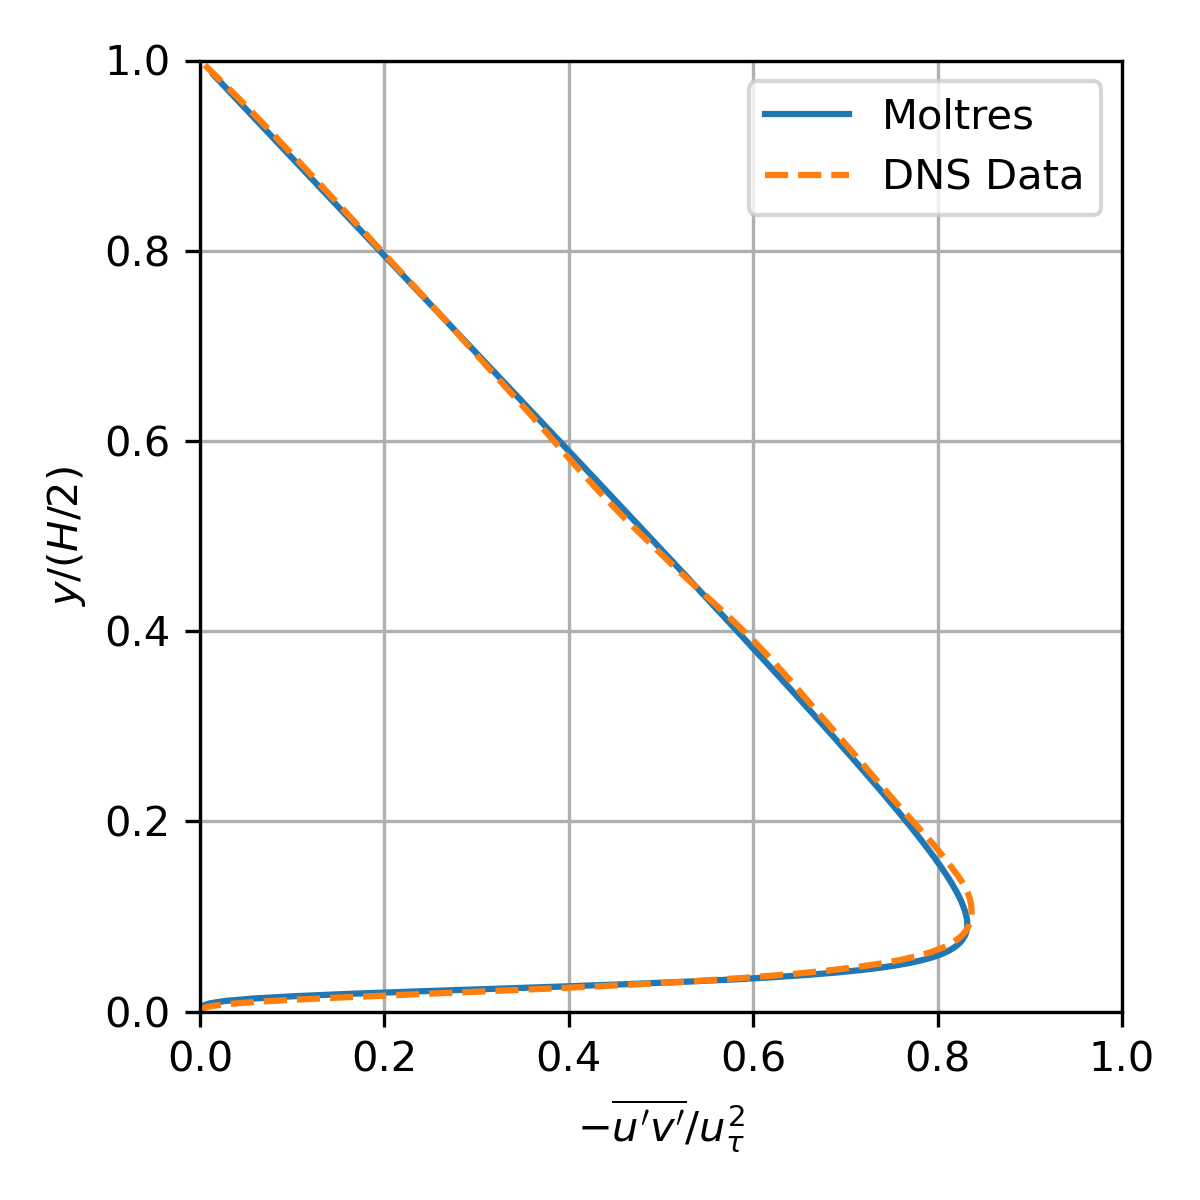
\includegraphics[width=\columnwidth]{channel_stress}
    \caption{Normalized stress distribution across the channel.}
    \label{fig:channel-stress}
  \end{subfigure}
  \caption{Comparison of turbulent channel flow results at Re$_\tau\approx395$ against reference
  \gls{DNS} results \cite{moser_direct_1999}. The Moltres Spalart-Allmaras model agrees consistently with
  the reference data.}
  \label{fig:channel-verification}
\end{figure}

\subsection{Turbulent Pipe Flow Validation Test}

In 1954, Laufer performed turbulent pipe flow experiments for Re $\approx 40000$
\cite{laufer_structure_1954}. Their results serve as the reference solution for this turbulent pipe
flow test.

\begin{figure}[p]
  \centering
  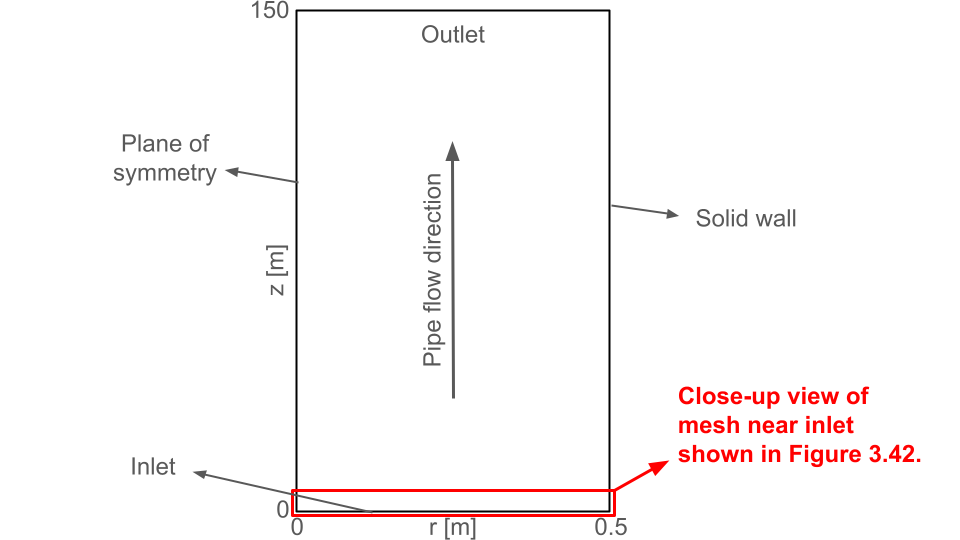
\includegraphics[width=0.8\columnwidth]{pipe-geom}
  \caption{Pipe geometry for the turbulent pipe flow verification test. The red box indicates
  the region shown by the close-up views in Figure \ref{fig:pipe-mesh}.}
  \label{fig:pipe-geom}
%\end{figure}
%%
%\begin{figure}[htb!]
  \centering
  \begin{subfigure}[b]{0.40\columnwidth}
    \centering
    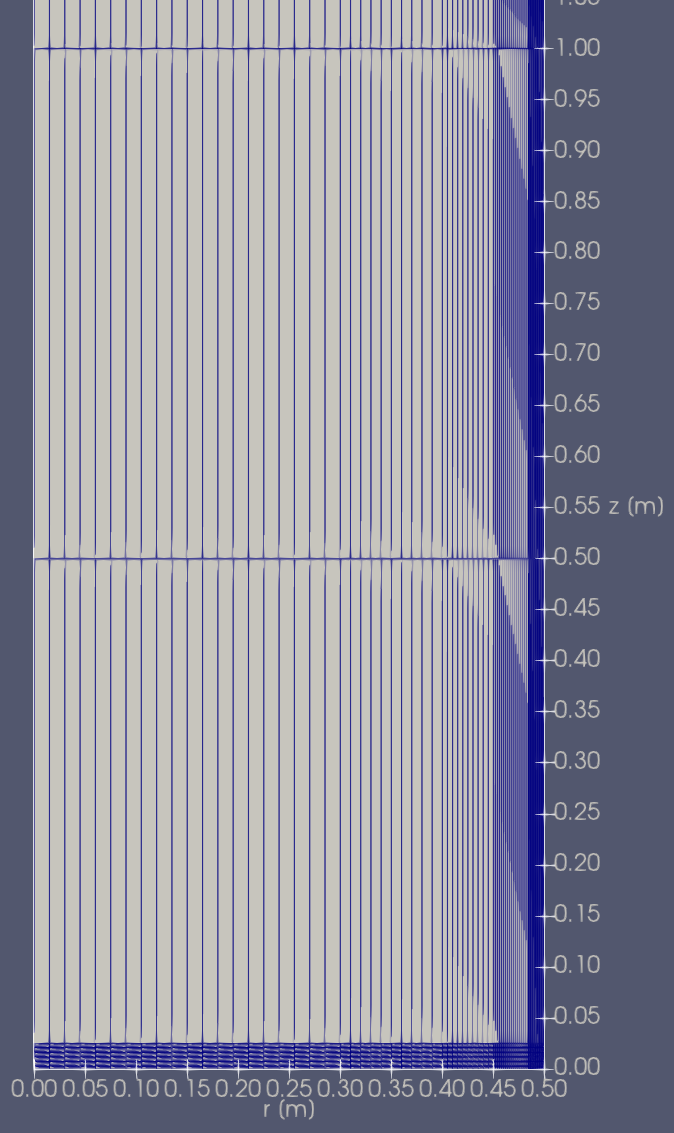
\includegraphics[width=\columnwidth]{pipe_mesh}
    \caption{Close-up view of the refined mesh near the inlet for the pipe flow test.}
    \label{fig:pipe-mesh-1}
  \end{subfigure}
  \hfill
  \begin{subfigure}[b]{0.53\columnwidth}
    \centering
    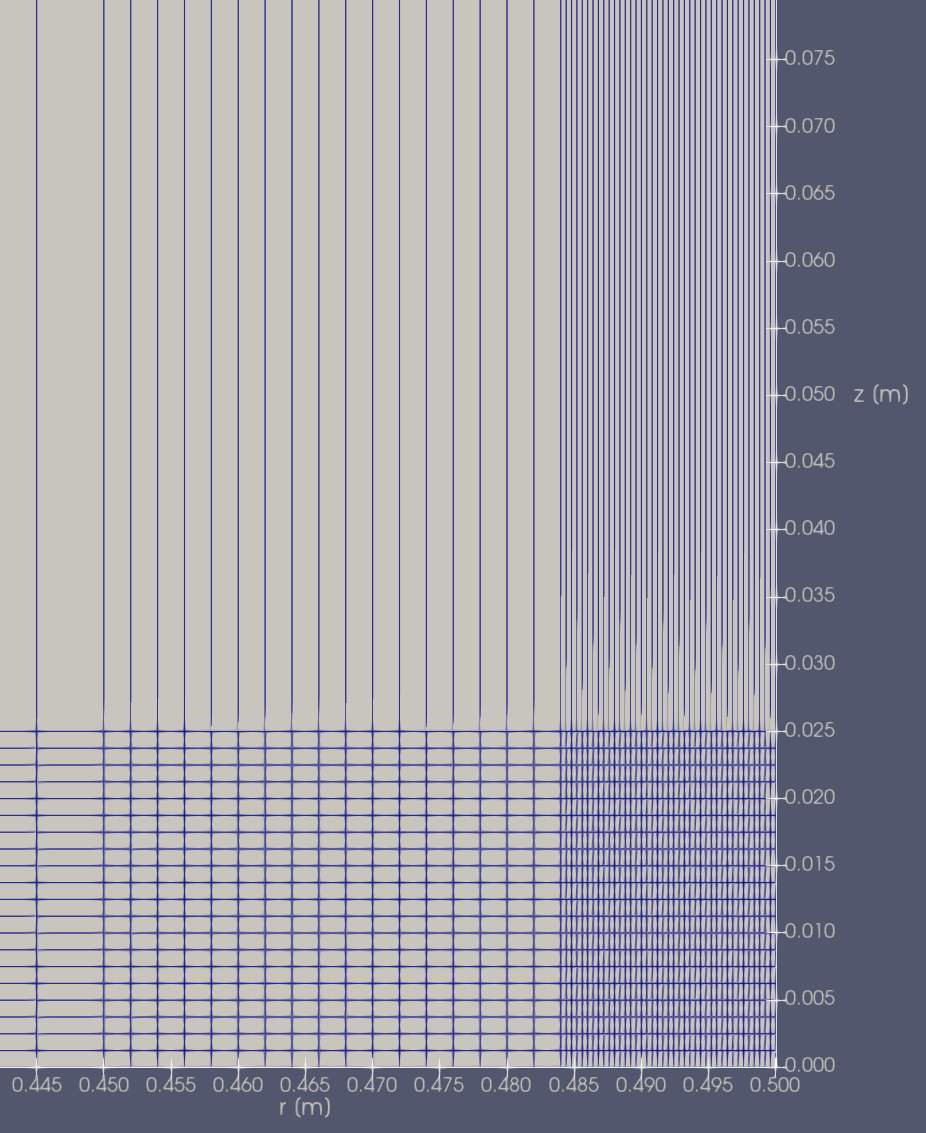
\includegraphics[width=\columnwidth]{pipe_mesh_zoom}
    \caption{Close-up view of the refined mesh near the inlet and wall boundary interface.}
    \label{fig:pipe-mesh-2}
  \end{subfigure}
  \caption{Close-up views of the refined mesh near the inlet (bottom boundary) and wall (right
  boundary). The mesh for the rest of the channel follows the mesh resolution of the topmost row of
  elements in the left subfigure.}
  \label{fig:pipe-mesh}
\end{figure}

The Moltres model for this test is a 2-D axisymmetric (R-Z coordinates) half-pipe with a radius of
0.5 m and a length of 150 m (Figure \ref{fig:pipe-geom}). The main flow direction
is in the positive $z$ direction with the inlet and outlet on the bottom and top ends,
respectively. The channel wall lies along the right boundary ($r=0.5$ m) while the left boundary
($r=0$ m) serves as a symmetry axis for the half-pipe geometry. Figure \ref{fig:pipe-mesh} shows
two close-up views of the refined mesh near the inlet and along the right wall boundary. The mesh
for the rest of the pipe geometry follows the same mesh resolution as the topmost row of
elements shown on the near the top of Figure \ref{fig:pipe-mesh-1}. The dimensionless wall distance
parameter $y^+$ of the first mesh element along wall boundary for fully developed flow at the end
of the pipe is 0.847, meeting the
$y^+ \lesssim 1$ requirement for properly wall-resolved flow. Table \ref{table:channel} lists
relevant flow parameters for the turbulent pipe flow test. The Moltres channel flow model ran as a
time-dependent simulation with adaptive time-stepping starting from a timestep size of 0.01
s up to a maximum timestep size of 10 s with a timestep size growth factor of 1.1. The simulation
automatically terminated at $t=165$ s when Moltres detected that the flow profile reached
steady-state, i.e., the flow and turbulent viscosity distributions remained unchanged between
successive timesteps.

\begin{table}[htb]
  \centering
  \small
  \caption{Relevant turbulent pipe flow problem parameters. The $\tilde{\mu}_\text{inlet}$ value
  at the inlet is set to fives times the $\mu$ value as recommended for the Spalart-Allmaras model
  \cite{spalart_one-equation_1994}.}
  \begin{tabular}{l S}
    \toprule
    Property & {Value} \\
    \midrule
    Density, $\rho$ [kg m$^{-3}$] & 1.0 \\
    Inlet velocity, $v_z$ [m s$^{-1}$] & 1.0 \\
    Dynamic viscosity, $\mu$ [kg m$^{-1}$ s$^{-1}$] & 2.5e-5 \\
    Reynolds number, Re [-] & 4.0e4 \\
    Modified viscosity along inlet, $\tilde{\mu}_\text{inlet}$ [kg m$^{-1}$ s$^{-1}$] & 1.25e-4 \\
    Modified viscosity along wall, $\tilde{\mu}_\text{wall}$ [kg m$^{-1}$ s$^{-1}$] & 0.0 \\
    \bottomrule
  \end{tabular}
  \label{table:pipe}
\end{table}

Figure \ref{fig:pipe-verification} shows plots of normalized and nondimensionalized velocities,
wall distances, and stresses from the experimental data \cite{laufer_structure_1954}
and the Moltres Spalart-Allmaras model. The Moltres Spalart-Allmaras model is largely consistent with the reference
experimental flow data and reproduces the expected trends in the velocity and stress distributions
across the channel and as a function of the wall distance.

\begin{figure}[htb]
  \centering
  \begin{subfigure}[b]{0.48\columnwidth}
    \centering
    \includegraphics[width=\columnwidth]{pipe_vel}
    \caption{Normalized velocity distribution across the pipe.}
    \label{fig:pipe-vel}
  \end{subfigure}
  \hfill
  \begin{subfigure}[b]{0.48\columnwidth}
    \centering
    \includegraphics[width=\columnwidth]{pipe_nondim}
    \caption{Dimensionless velocity vs.\ dimensionless wall distance}
    \label{fig:pipe-nondim}
  \end{subfigure}
  \begin{subfigure}[b]{0.48\columnwidth}
    \centering
    \includegraphics[width=\columnwidth]{pipe_stress}
    \caption{Normalized turbulent shear stress distribution across the pipe.}
    \label{fig:pipe-stress}
  \end{subfigure}
  \caption{Comparison of turbulent pipe flow results at Re $\approx 40000$ against reference
  experimental data \cite{laufer_structure_1954}.}
  \label{fig:pipe-verification}
\end{figure}

\FloatBarrier

\subsection{Backward-Facing Step Flow Validation Test}

Driver \& Seegmiller performed the \gls{BFS} flow experiment for Re $\approx36000$ (based on the
step height)
\cite{driver_features_1985}. Their results serve as the reference solution for this \gls{BFS} test.
Additionally, the \gls{NASA} Turbulence Modeling Resource website \cite{rumsey_turbulence_nodate}
provides \gls{BFS} simulation results generated from the regular Spalart-Allmaras model in the CFL3D
Navier-Stokes CFD code developed at \gls{NASA} \cite{krist_cfl3d_1998}. The CFL3D Spalart-Allmaras model
does not contain the rotation correction scheme
\cite{aupoix_extensions_2003, dacles-mariani_numericalexperimental_1995} present in the Moltres
Spalart-Allmaras model.

\begin{figure}[p]
  \centering
  \includegraphics[width=0.9\columnwidth]{backstep-geom}
  \caption{Backward step geometry for the turbulent \gls{BFS} flow verification test. The red box indicates
  the region shown by the close-up view in Figure \ref{fig:bfs-mesh}.}
  \label{fig:backstep-geom}
%\begin{figure}[htb!]
  \centering
  \includegraphics[width=0.9\columnwidth]{bfs_mesh}
  \caption{Close-up view of the mesh for the \gls{BFS} flow test. The step is situated at $x=110$ m
  with a height of $H=1$ m.}
  \label{fig:bfs-mesh}
\end{figure}

The Moltres model for this test is a 2-D 160 m-long channel (Figure \ref{fig:backstep-geom}.
The main flow direction is in the
positive $x$ direction with the inlet and outlet on the left and right ends, respectively. The
channel is 8 m tall before the 1 m-tall step at $x=110$ m. Figure \ref{fig:bfs-mesh} shows a
close-up view of the mesh around the step. The dimensionless wall distance parameter $y^+$ of the
first mesh elements along wall boundaries just prior to the step and at the end of the channel are
0.735 and 0.555, respectively, meeting the $y^+ \lesssim 1$ requirement for properly wall-resolved
flow. Table \ref{table:bfs} lists relevant flow parameters for the turbulent \gls{BFS} flow test.
The Moltres \gls{BFS} flow model ran as two separate simulations for the upstream turbulent flow
profile to fully develop from $x=0$ m to $x=104$ m and the \gls{BFS} flow profile from $x=104$ m to
$x=160$ m. The fully-developed flow profile at $x=104$ m from the first simulation served as the
inlet flow profile for the second simulation. Both simulations ran with adaptive time-stepping
starting from a timestep size of 0.1 s up to a maximum timestep size of 10 s with a timestep size
growth factor of 1.1. The upstream and \gls{BFS} simulations automatically terminated at $t=212$ s
and $t=223$ s when Moltres detected that the flow profiles reached steady-state.

\begin{table}[htb]
  \centering
  \small
  \caption{Relevant turbulent \gls{BFS} flow problem parameters. The $\tilde{\mu}_\text{inlet}$ value
  at the inlet is set to fives times the $\mu$ value as recommended for the Spalart-Allmaras model
  \cite{spalart_one-equation_1994}.}
  \begin{tabular}{l S}
    \toprule
    Property & {Value} \\
    \midrule
    Density, $\rho$ [kg m$^{-3}$] & 1.0 \\
    Inlet velocity, $v_z$ [m s$^{-1}$] & 1.0 \\
    Dynamic viscosity, $\mu$ [kg m$^{-1}$ s$^{-1}$] & 2.778e-5 \\
    Reynolds number based on step height $H=1$ m, Re$_H$ [-] & 3.6e4 \\
    Modified viscosity along inlet, $\tilde{\mu}_\text{inlet}$ [kg m$^{-1}$ s$^{-1}$] & 1.389e-4 \\
    Modified viscosity along wall, $\tilde{\mu}_\text{wall}$ [kg m$^{-1}$ s$^{-1}$] & 0.0 \\
    \bottomrule
  \end{tabular}
  \label{table:bfs}
\end{table}

Figure \ref{fig:bfs} shows the velocity magnitude and streamlines around the step at $x=110$ m. The
streamlines illustrate the recirculation zones created by flow separation past the step.
Figure \ref{fig:bfs-plots} shows the normalized velocity distributions at various distances from
step, the skin friction and skin pressure coefficients along the bottom wall, and the normalized
turbulent shear stress distributions at various distances downstream of the step. The Spalart-Allmaras
model with the rotation correction scheme in Moltres performs largely similarly to the reference
Spalart-Allmaras model results provided on the \gls{NASA} Turbulence Modeling Resource website
\cite{rumsey_turbulence_nodate}. Compared with the reference experimental data, the Moltres
Spalart-Allmaras model predicts more accurate velocity (Figure \ref{fig:bfs-downstream}) and turbulent
stress distributions (Figure \ref{fig:bfs-stress}) along $x/H=1$ downstream of the
step than the CFL3D Spalart-Allmaras model. This indicates that the Moltres
Spalart-Allmaras model reproduces the sizes and shapes of the largest and second-largest recirculation
zones (see Figure \ref{fig:bfs}) more accurately than the CFL3D Spalart-Allmaras model. Table
\ref{table:bfs-reattach} further supports the prior observation since the flow reattachment length
estimate from Moltres is more consistent with the experimental data than CFL3D. The Moltres
Spalart-Allmaras velocity distributions in Figure \ref{fig:bfs-downstream} are largely consistent with the
experimental data. Lastly, the reader should
note that this turbulent \gls{BFS} flow setup induces complex flow separation effects despite the
apparent simplicity of the geometry. All \gls{RANS}-based model results from the \gls{NASA}
turbulence modeling resource website \cite{rumsey_turbulence_nodate} fail to accurately reproduce
the turbulent shear stress distribution (Figure \ref{fig:bfs-stress}) from the reference
experimental data. Therefore, the discrepancies observed in the turbulent shear stresses from the
Spalart-Allmaras model are within expectations of a \gls{RANS}-based model.

\begin{table}[htb]
  \centering
  \small
  \caption{\gls{BFS} flow reattachment length estimates normalized by step height $H$.}
  \begin{tabular}{l S[table-format=1.2(2)]}
    \toprule
    Source & {Reattachment length [-]} \\
    \midrule
    Experimental data \cite{driver_features_1985} & 6.26(10) \\
    CFL3D Spalart-Allmaras model \cite{rumsey_turbulence_nodate} & 6.1 \\
    Moltres Spalart-Allmaras model & 6.36 \\
    \bottomrule
  \end{tabular}
  \label{table:bfs-reattach}
\end{table}

\begin{figure}[htb!]
  \centering
  \includegraphics[width=\columnwidth]{bfs}
  \caption{Velocity magnitude distribution and streamlines around the backward-facing step. The
  streamlines illustrate the primary and secondary recirculation zones induced by flow past the
  step.}
  \label{fig:bfs}
\end{figure}

\begin{figure}[htb]
  \centering
  \hfill
  \begin{subfigure}[b]{0.38\columnwidth}
    \centering
    \includegraphics[width=\columnwidth]{bfs_upstream_vel}
    \caption{Normalized velocity distribution at $x/H=-4$ upstream of step.}
    \label{fig:bfs-upstream}
  \end{subfigure}
  \hfill
  \begin{subfigure}[b]{0.38\columnwidth}
    \centering
    \includegraphics[width=\columnwidth]{bfs_downstream_vel}
    \caption{Normalized velocity distributions downstream of step.}
    \label{fig:bfs-downstream}
  \end{subfigure} \hfill \\
  \centering
  \hfill
  \begin{subfigure}[b]{0.38\columnwidth}
    \centering
    \includegraphics[width=\columnwidth]{bfs_cf}
    \caption{Skin friction coefficient along the bottom wall.}
    \label{fig:bfs-cf}
  \end{subfigure}
  \hfill
  \begin{subfigure}[b]{0.38\columnwidth}
    \centering
    \includegraphics[width=\columnwidth]{bfs_cp}
    \caption{Skin pressure coefficient along the bottom wall.}
    \label{fig:bfs-cp}
  \end{subfigure} \hfill \\
  \centering
  \begin{subfigure}[b]{0.38\columnwidth}
    \centering
    \includegraphics[width=\columnwidth]{bfs_stress}
    \caption{Normalized turbulent shear stress distributions downstream
    of step.}
    \label{fig:bfs-stress}
  \end{subfigure}
  \caption{Comparison of backward facing step flow results against reference
  experimental data and computational data from CFL3D. $x/H$ values are normalized horizontal
  distances relative to the step.}
  \label{fig:bfs-plots}
\end{figure}

\subsection{Summary}

\glspl{MSR} feature turbulent flow along various sections of the primary molten salt loop which in
turn induce turbulent temperature and \glspl{DNP} transport. This section presented the
implementation, verification, and validation of the Spalart-Allmaras turbulence model
\cite{spalart_one-equation_1994} in Moltres for turbulence
modeling capabilities. The one-equation \gls{RANS}-based Spalart-Allmaras model is computationally
efficient relative to more complex \gls{RANS}-based and high-fidelity models while providing better
accuracy than algebraic models when modeling flows with flow separation and significant streamline
curvatures \cite{wilcox_turbulence_2006}.

Verification and validation results for turbulent channel, pipe, and \gls{BFS} flow tests showed
that the Moltres Spalart-Allmaras model is largely consistent with reference simulation or experimental
data in the literature. The Moltres Spalart-Allmaras model includes a rotation correction scheme
\cite{aupoix_extensions_2003, dacles-mariani_numericalexperimental_1995} and notably outperforms
the CFL3D Spalart-Allmaras model in the turbulent \gls{BFS} flow test with more accurate velocity
distributions and flow reattachment length estimate.


\glsresetall

\chapter{Hybrid $S_N$-Diffusion Method}
\label{chap:hybrid}
Section \ref{sec:summary-nts-mtds} highlights the poor performance of neutron diffusion
methods for calculating neutron fluxes near control rods. Strong neutron absorption in the control
rod region produces a highly anisotropic neutron flux extending some distance outside the control
rod. Neutron transport methods, which retain angular dependence of the neutron flux to various
extents, generally fare better than neutron diffusion methods, which have isotropic diffusion
coefficients. However, neutron transport methods are also generally more computationally expensive,
given the increased dimensionality of the problem from the angular component. Adding an angular
dimension to the existing geometric and neutron energy group dimensions dramatically
increases the problem size and the computational resources necessary to solve the system. Many past
efforts have tried introducing
transport correction techniques to improve neutron flux and multiplication factor estimates in
diffusion-based methods. Other than control rod regions, these techniques may also correct
homogenization errors introduced by spatial homogenization of fuel assemblies and other
structures within a reactor core. They invariably rely on neutron transport methods to generate
transport corrections in the form of corrected diffusion coefficients
\cite{bretscher_computing_1997, scherer_determination_1976, ronen_accurate_2004,
pounders_diffusion_2009, kavenoky_sph_1978}, boundary conditions \cite{davison_influence_1951,
pellaud_extrapolation_1968, fen_modelling_1992}, Eddington factors, or discontinuity factors
\cite{koebke_new_1980}.

In this chapter, I propose a hybrid $S_N$-diffusion neutronics method to improve control rod
modeling in neutron diffusion solvers without spatial homogenization. In essence, the hybrid
method is an iterative method that applies
the $S_N$ discrete ordinates neutron transport method on subregions containing the control rod to
obtain pointwise transport corrections for the diffusion method on the subregions.
This chapter presents the mathematical derivation for the
\gls{SAAF} formulation of the $S_N$ equations and the drift transport correction term for the
neutron diffusion equations, and the computational algorithm for the hybrid method.

Section \ref{sec:saaf} provides the mathematical derivation for the discretized weak form of the
\gls{SAAF} $S_N$ neutron transport equations. Section \ref{sec:transport-correction} provides the
derivations for the transport correction formulations I investigated for use in the hybrid method.
Section \ref{sec:hybrid-algorithm} details the iteration algorithm for the hybrid method. Section
\ref{sec:sn-bc} provides the boundary conditions formulated for the $S_N$ calculations in the
hybrid method. In Section \ref{sec:buffer-region}, I discuss how transport corrections are handled
in the hybrid method. Lastly, Section \ref{sec:hybrid-summary} summarizes the hybrid method and its
implementation.

% Section \ref{sec:theory} discusses the theoretical background for the hybrid $S_N$-diffusion
% method. Section \ref{sec:implementation} provides numerical implementation details of
% the hybrid method and its components. Sections \ref{sec:test-case} and \ref{sec:sim-param} describe
% the 1-D test cases and several simulation parameters in that context. Section
% \ref{sec:prelim-results} discusses the results of the hybrid method applied to the 1-D test cases
% with comparisons to higher-fidelity Monte Carlo and $S_N$ neutron transport methods. Lastly,
% Section \ref{sec:hybrid-summary} summarizes the key findings in this chapter.

\section{\Gls{SAAF} $S_N$ Method} \label{sec:saaf}

This chapter starts with the $S_N$ method implementation required for the hybrid $S_N$-diffusion
method. I implemented both $S_N$ and hybrid methods using \gls{FEM} numerical solver capabilities
available through Moltres \cite{lindsay_moltres_2017} and the \gls{MOOSE} framework. In this
section, the derivation for the \gls{SAAF} formulation of the $S_N$ method and its
implementation in Moltres follows closely the derivation developed by Wang et al.\
\cite{wang_diffusion_2014, wang_rattlesnake_2018}.

\subsection{Multigroup Neutron Transport Equations}

Continuing from the introduction to neutronics methods in Section \ref{sec:summary-nts-mtds},
the time-dependent, multigroup neutron transport equation defined on the 3-D spatial domain
$\mathcal{D}$ and 2-D unit sphere angular domain $\mathcal{S}$ is:
%
\begin{multline}
  \frac{\partial}{\partial t}\left[\frac{\Psi_g(\vec{r},\hat{\Omega},t)}{v_g}\right] +
  \hat{\Omega}\cdot\nabla\Psi_g(\vec{r},\hat{\Omega},t) + \Sigma_{t,g}
  \Psi_g(\vec{r},\hat{\Omega},t) =
  \sum^G_{g'=1}\int_\mathcal{S} \Sigma_s^{g'\rightarrow g}(\hat{\Omega}'\rightarrow\hat{\Omega})
  \Psi_{g'}(\vec{r},\hat{\Omega}',t)d\hat{\Omega}' \\
  + \frac{1}{4\pi}\chi_{p,g}(1-\beta)\sum^G_{g'=1} \nu\Sigma_{f,g'} \phi_{g'}(\vec{r},t)
  + \frac{1}{4\pi}\sum^I_{i=1}\chi_{d,g}
  \lambda_i C_i(\vec{r},t) + Q^{\text{ext}}_g(\vec{r},\hat{\Omega})
  \label{eq:mg-nte}
\end{multline}
%
with the boundary conditions
%
\begin{gather}
  \Psi_g(\vec{r},\hat{\Omega}) = \Psi^\text{inc}_g(\vec{r},\hat{\Omega}) +
  \alpha^s_g\Psi_g(\vec{r},\hat{\Omega}_r)
  \mbox{ on } \vec{r} \in \partial\mathcal{D} \mbox{ and } \hat{\Omega}\cdot\hat{n}_b < 0,
  \shortintertext{where}
  \begin{align*}
    \chi_{p,g} &= \mbox{prompt fission neutron spectrum in group $g$,} \\
    \beta &= \sum^I_{i=1} \beta_i = \mbox{total delayed neutron fraction,} \\
    \chi_{d,g} &= \mbox{delayed fission neutron spectrum in group $g$,} \\
    \lambda_i &= \mbox{decay constant of precursor group $i$,} \\
    C_i &= \mbox{delayed neutron precursor concentration for group $i$,} \\
    \Psi^\text{inc}_g &= \mbox{incident surface source in group $g$,} \\
    \alpha^s_g &= \mbox{specular reflectivity on }\partial \mathcal{D} \mbox{ for group }g, \\
    \hat{\Omega}_r &= \hat{\Omega}-2(\hat{\Omega}\cdot \hat{n}_b)\hat{n}_b, \\
    \hat{n}_b &= \mbox{outward unit normal vector on the boundary.}
  \end{align*}
\end{gather}
%
In order to introduce operators and facilitate subsequent mathematical derivations, we will define
the following vector forms:
%
\begin{gather}
  \bm{\Psi} \equiv
  \begin{bmatrix}
    \Psi_1 \\
    \Psi_2 \\
    \vdots \\
    \Psi_G
  \end{bmatrix},
  \bm{\Phi} \equiv \int_S \bm{\Psi}d\hat{\Omega} \equiv
  \begin{bmatrix}
    \phi_1 \\
    \phi_2 \\
    \vdots \\
    \phi_G
  \end{bmatrix},
  \bm{\frac{\Psi}{v}} \equiv
  \begin{bmatrix}
    \frac{\Psi_1}{v_1} \\
    \frac{\Psi_2}{v_2} \\
    \vdots \\
    \frac{\Psi_G}{v_G}
  \end{bmatrix},
  \bm{C} \equiv
  \begin{bmatrix}
    C_1 \\
    C_2 \\
    \vdots \\
    C_G
  \end{bmatrix},
  \bm{Q}^{\text{ext}} \equiv
  \begin{bmatrix}
    Q^\text{ext}_1 \\
    Q^\text{ext}_2 \\
    \vdots \\
    Q^\text{ext}_G
  \end{bmatrix}, \nonumber
%  \bm{Q}_f = \frac{1}{4\pi}\bm{Q}_{f,0} =
%  \begin{bmatrix}
%    \frac{1}{4\pi}\chi_{p,1}(1-\beta)\sum^G_{g'=1} \nu\Sigma_{f,g'} \phi_{g'} +
%    \frac{1}{4\pi}\sum^I_{i=1}\chi_{d,1} \lambda_i C_i \\
%    \frac{1}{4\pi}\chi_{p,2}(1-\beta)\sum^G_{g'=1} \nu\Sigma_{f,g'} \phi_{g'} +
%    \frac{1}{4\pi}\sum^I_{i=1}\chi_{d,2} \lambda_i C_i \\
%    \vdots \\
%    \frac{1}{4\pi}\chi_{p,G}(1-\beta)\sum^G_{g'=1} \nu\Sigma_{f,g'} \phi_{g'} +
%    \frac{1}{4\pi}\sum^I_{i=1}\chi_{d,G} \lambda_i C_i
%  \end{bmatrix},
%  \bm{Q} = \bm{Q}_f + \bm{Q}^\text{ext}. \nonumber
\end{gather}
%
We also define the following operators:
%
\begin{gather}
  \mathbb{L}_1\bm{\Psi} \equiv
  \begin{bmatrix}
    \hat{\Omega}\cdot\nabla\Psi_1 \\
    \hat{\Omega}\cdot\nabla\Psi_2 \\
    \vdots \\
    \hat{\Omega}\cdot\nabla\Psi_G \\
  \end{bmatrix},
  \mathbb{L}_2\bm{\Psi} \equiv
  \begin{bmatrix}
    \Sigma_{t,1}\Psi_1 \\
    \Sigma_{t,2}\Psi_2 \\
    \vdots \\
    \Sigma_{t,G}\Psi_G
  \end{bmatrix},
  \mathbb{L}\bm{\Psi} \equiv \mathbb{L}_1\bm{\Psi} + \mathbb{L}_2\bm{\Psi}, \nonumber \\
  \mathbb{S}\bm{\Psi} \equiv
  \begin{bmatrix}
    \sum^G_{g'=1}\int_S \Sigma_s^{g'\rightarrow 1}\Psi_{g'}d\hat{\Omega} \\
    \sum^G_{g'=2}\int_S \Sigma_s^{g'\rightarrow 2}\Psi_{g'}d\hat{\Omega} \\
    \vdots \\
    \sum^G_{g'=G}\int_S \Sigma_s^{g'\rightarrow G}\Psi_{g'}d\hat{\Omega}
  \end{bmatrix},
  \mathbb{B}\bm{\Psi} \equiv
  \begin{bmatrix}
    \alpha^s_1\Psi_1(\hat{\Omega}_r) \\
    \alpha^s_2\Psi_2(\hat{\Omega}_r) \\
    \vdots \\
    \alpha^s_G\Psi_G(\hat{\Omega}_r)
  \end{bmatrix}, \nonumber \\
  \mathbb{F}\bm{\Psi} \equiv \frac{1}{4\pi}\mathbb{F}_0\bm{\Psi} \equiv
  \begin{bmatrix}
    \frac{1}{4\pi}\chi_{p,1}(1-\beta)\sum^G_{g'=1}\nu\Sigma_{f,g'}\phi_{g'} \\
    \frac{1}{4\pi}\chi_{p,2}(1-\beta)\sum^G_{g'=1}\nu\Sigma_{f,g'}\phi_{g'} \\
    \vdots \\
    \frac{1}{4\pi}\chi_{p,G}(1-\beta)\sum^G_{g'=1}\nu\Sigma_{f,g'}\phi_{g'}
  \end{bmatrix},
  \mathbb{C}\bm{C} \equiv \frac{1}{4\pi}\mathbb{C}_0\bm{C} \equiv
  \begin{bmatrix}
    \frac{1}{4\pi}\sum^I_{i=1}\chi_{d,1} \lambda_i C_i \\
    \frac{1}{4\pi}\sum^I_{i=1}\chi_{d,2} \lambda_i C_i \\
    \vdots \\
    \frac{1}{4\pi}\sum^I_{i=1}\chi_{d,G} \lambda_i C_i
  \end{bmatrix}. \nonumber
\end{gather}
%
Note that the operators apply element-wise multiplication as opposed to the more conventional
matrix multiplication. Eq.\ \ref{eq:mg-nte} can be reexpressed as:
%
\begin{gather}
  \frac{\partial}{\partial t} \left(\frac{\bm{\Psi}}{\bm{v}}\right)+\mathbb{L}\bm{\Psi}
  = \mathbb{S}\bm{\Psi} + \bm{Q}, \label{eq:nte-vec}
\end{gather}
%
with the boundary conditions on $\partial\mathcal{D}$
%
\begin{gather}
  \bm{\Psi} = \bm{\Psi}^\text{inc} + \mathbb{B}\bm{\Psi},
  \shortintertext{where}
  \begin{align*}
    \bm{Q} &= \bm{Q}_f + \bm{Q}^\text{ext}, & \\
    \bm{Q}_f &= \mathbb{F}\bm{\Psi} + \mathbb{C}\bm{C}. &
  \end{align*}
\end{gather}

\subsection{Weak Form of the Multigroup Neutron Transport Equations}

Before we begin the derivation for the \gls{SAAF} formulation, we introduce inner product notations
to express Eq.\ \ref{eq:nte-vec} and the eventual \gls{SAAF} formulation in their weak forms to be
solved using \gls{FEM}. We define the inner product consisting of volume integrals on
$\mathcal{D}\otimes\mathcal{S}$ as
%
\begin{gather}
  (\bm{a}, \bm{b})_{\mathcal{D}\otimes\mathcal{S}} \equiv
  \sum^G_{g=1}\int_\mathcal{S}d\hat{\Omega}\int_\mathcal{D}d\vec{r}\
  a_g(\vec{r},\hat{\Omega}) b_g(\vec{r},\hat{\Omega}), \label{eq:weak-domain}
\end{gather}
%
where $\bm{a}$ and $\bm{b}$ represent multigroup function vectors such as $\bm{\Psi}$. We also
define boundary integrals on $\partial\mathcal{D}\otimes\mathcal{S}$ as
%
\begin{gather}
  \langle\bm{a},\bm{b}\rangle^\pm_{\partial\mathcal{D}\otimes\mathcal{S}} \equiv
  \sum^G_{g=1}\int_{\partial\mathcal{D}}d\vec{r}
  \int_{\mathcal{S}^{\pm}}d\hat{\Omega}\ |\hat{\Omega}\cdot\hat{n}_b|
  a_g(\vec{r},\hat{\Omega}) b_g(\vec{r},\hat{\Omega}), \label{eq:weak-boundary}
\end{gather}
%
where the $\pm$ sign depends on the signedness of $\hat{\Omega}\cdot\hat{n}_b$ at the boundary.
We henceforth drop the phase space subscripts for brevity.
%
In accordance with standard weak form derivation procedure, we multiply Eq.\ \ref{eq:nte-vec}
by a test function $\bm{\Psi}^*$ and integrate throughout over the $\mathcal{D}$ and $\mathcal{S}$
domains
%
\begin{gather}
  \left(\bm{\Psi}^*,\frac{\partial}{\partial t}\left(\frac{\bm{\Psi}}{\bm{v}}\right)\right) +
  \left(\bm{\Psi}^*,\mathbb{L}\bm{\Psi}\right) = \left(\bm{\Psi}^*,\mathbb{S}\bm{\Psi}\right) +
  \left(\bm{\Psi}^*,\bm{Q}\right).
\end{gather}
%
We apply integration by parts on the streaming term to obtain
%
\begin{gather}
  \left(\bm{\Psi}^*,\frac{\partial}{\partial t}\left(\frac{\bm{\Psi}}{\bm{v}}\right)\right) +
  \left(\mathbb{L}^*\bm{\Psi}^*,\bm{\Psi}\right) + \langle\bm{\Psi}^*,\bm{\Psi}\rangle^+ -
  \langle\bm{\Psi}^*,\bm{\Psi}\rangle^- = \left(\bm{\Psi}^*,\mathbb{S}\bm{\Psi}\right) +
  \left(\bm{\Psi}^*,\bm{Q}\right), \label{eq:nte-weak}
\end{gather}
%
where $\mathbb{L}^*$ is the adjoint of $\mathbb{L}$.
%\begin{multline}
%  \left(\bm{\Psi}^*,\left(\mathbb{I} - \mathbb{L}^{-1}_2\mathbb{L}_1\right)
%  \frac{\partial}{\partial t}\left(\frac{\bm{\Psi}}{\bm{v}}\right)\right) -
%  \left(\mathbb{L}^*_1\bm{\Psi}^*,\mathbb{L}^{-1}_2\mathbb{L}_1\bm{\Psi}\right) +
%  \langle\bm{\Psi}^*,
%  \left(\bm{\Psi}^*,\mathbb{L}_2\bm{\Psi}\right) = \\
%  \left(\bm{\Psi}^*,\left(\mathbb{I} - \mathbb{L}^{-1}_2\mathbb{L}_1\right)\mathbb{S}\bm{\Psi}
%  \right) +
%  \left(\bm{\Psi}^*,\left(\mathbb{I} - \mathbb{L}^{-1}_2\mathbb{L}_1\right) \bm{Q}\right).
%\end{multline}

\subsection{\gls{SAAF} Formulation}

We begin the derivation for the \gls{SAAF} formulation by first rearranging Eq.\ \ref{eq:nte-vec}
as
%
\begin{gather}
  \bm{\Psi} = \mathbb{L}^{-1}_2\left[\mathbb{S}\bm{\Psi}+\bm{Q}
  -\frac{\partial}{\partial t}\left(\frac{\bm{\Psi}}{\bm{v}}\right)-\mathbb{L}_1\bm{\Psi}\right]
  \label{eq:afe}
  \shortintertext{where}
  \mathbb{L}^{-1}_2 =
  \begin{bmatrix}
    \frac{1}{\Sigma_{t,1}} \\
    \frac{1}{\Sigma_{t,2}} \\
    \vdots \\
    \frac{1}{\Sigma_{t,G}}
  \end{bmatrix}. \nonumber
\end{gather}
%
We substitute Eq.\ \ref{eq:afe} back into the streaming term in Eq.\ \ref{eq:nte-weak} and
rearrange the terms to obtain
%
\begin{multline}
  \left(\mathbb{L}^{-1}_2\mathbb{L}\bm{\Psi}^*,\frac{\partial}{\partial t}\left(\frac{\bm{\Psi}}
      {\bm{v}}\right)\right) + 
  \left(\mathbb{L}_1\bm{\Psi}^*,\mathbb{L}^{-1}_2\mathbb{L}_1\bm{\Psi}\right) +
  \langle\bm{\Psi}^*,\bm{\Psi}\rangle^+ - \langle\bm{\Psi}^*,\bm{\Psi}\rangle^- +
  \left(\mathbb{L}_2\bm{\Psi}^*,\bm{\Psi}\right) = \\
  \left(\mathbb{L}^{-1}_2\mathbb{L}\bm{\Psi}^*,
  \mathbb{S}\bm{\Psi}\right) + \left(\mathbb{L}^{-1}_2\mathbb{L}\bm{\Psi}^*,\bm{Q}\right)
  \label{eq:saaf}
\end{multline}
%
using the following relations
%
\begin{gather}
  \mathbb{L}_1\mathbb{L}_2 = \mathbb{L}_2\mathbb{L}_1, \hspace{1cm}
  \mathbb{L}^*_1 = -\mathbb{L}_1,\hspace{1cm}
  \mathbb{L}^*_2 = \mathbb{L}_2, \nonumber \\
  \mathbb{I}-\mathbb{L}^{-1}_2\mathbb{L}^*_1 =
  \mathbb{L}^{-1}_2\mathbb{L}_2 + \mathbb{L}^{-1}_2\mathbb{L}_1 =
  \mathbb{L}^{-1}_2\mathbb{L}. \nonumber
\end{gather}

Notably, the \gls{SAAF} formulation contains a second-order derivative streaming term
(prior to applying integration by parts) which lends itself better to standard
\gls{FEM} solver routines, such as the \gls{GMRES} method, than the first-order streaming
term of the original formulation.
However, the $\mathbb{L}^{-1}_2$ operators render the current \gls{SAAF} formulation
unsolveable in void and near-void regions where the total cross sections $\Sigma_{t,g}$ approach
zero \cite{wang_diffusion_2014}.

\subsection{Spatial Discretization and Void Treatment} \label{sec:void-treatment}

To overcome the issue of voids, Wang et al.\ \cite{wang_diffusion_2014} modified the standard
\gls{SAAF} formulation by taking inspiration from the \gls{SUPG} stabilization technique
\cite{brooks_streamline_1982}. We start by first applying spatial discretization on the \gls{SAAF}
formulation. For \gls{FEM}, the spatial domain is discretized into finite, non-overlapping mesh
elements $\mathcal{D}_e$ such that $\mathcal{D} = \cup_{e\in\mathbb{T}_h}\mathcal{D}_e$, where
$\mathbb{T}_h$ denotes the index set of elements discretizing $\mathcal{D}$ and $\mathcal{D}_e$
is the subdomain covered by the element of index $e$. Similarly, the outermost boundary
$\partial\mathcal{D}$ is discretized by non-overlapping mesh sides indexed by $s$. Within each mesh
element, any spatially varying function can be approximated with basis functions
%
\begin{gather}
  f(\vec{r}) = \sum^N_{i=1}f_i b_i(\vec{r}),
  \shortintertext{where}
  \begin{align*}
    N &= \mbox{degrees of freedom in the mesh element,} \\
    b_i &= \mbox{basis function,} \\
    f_i &= \mbox{coefficient corresponding to $b_i$ in approximating $f$}.
  \end{align*}
\end{gather}

Thus, we can define the inner products
%
\begin{gather}
  \left(\bm{a},\bm{b}\right) \equiv \sum^G_{g=1}\int_\mathcal{S}d\hat{\Omega}
  \sum_{e\in\mathbb{T}_h}\int_{\mathcal{D}_e}d\vec{r}\sum_{i\in E_e}a_{g,i}(\hat{\Omega})
  b_i(\vec{r})\sum_{j\in E_e}b_{g,j}(\hat{\Omega})b_j(\vec{r}), \\
  \langle\bm{a},\bm{b}\rangle^{\pm} \equiv \sum^G_{g=1}\sum_{s\in\partial\mathcal{D}}\int_s
  d\vec{r} \int_{mathcal{S}^\pm_{\hat{n}_b}}d\hat{\Omega} |\hat{\Omega}\cdot\hat{n}_b|
  \sum_{i\in E_s}a_{g,i}(\hat{\Omega})b_i(\vec{r})\sum_{j\in E_s}b_{g,j}(\hat{\Omega})b_j(\vec{r}),
  \shortintertext{where}
  \begin{align*}
    E_e &= \mbox{index set of the local basis functions in element $e$,} \\
    E_s &= \mbox{index set of the local basis functions in element side $s$,}
  \end{align*}
\end{gather}
%
to apply spatial discretization on Eq.\ \ref{eq:saaf} by replacing the preexisting inner product
notations defined in Eqs.\ \ref{eq:weak-domain} and \ref{eq:weak-boundary}.

We can now proceed with the void treatment for stabilization.
We start by defining the following stabilization operator
%
\begin{gather}
  \bm{\tau} \equiv
  \begin{bmatrix}
    \tau_1 \\
    \tau_2 \\
    \vdots \\
    \tau_G
  \end{bmatrix}
  \shortintertext{where}
  \begin{align*}
    \tau_g &=
    \begin{cases}
      \frac{1}{c\Sigma_{t,g}} \mbox{ for } ch\Sigma_{t,g} \geq \varsigma \\
      \frac{h}{\varsigma} \mbox{ for } ch\Sigma_{t,g} < \varsigma
    \end{cases}, & \\
    h &= \mbox{mesh element size,} & \\
    c &= \mbox{maximum stabilization factor,} & \\
    \varsigma &= \mbox{void constant.} &
  \end{align*}
\end{gather}
%
Next, we redefine Eq.\ \ref{eq:afe} as
%
\begin{gather}
  \bm{\Psi} = \left(\mathbb{I}-\bm{\tau}\mathbb{L}_2\right)\bm{\Psi}+
  \bm{\tau}\left[\mathbb{S}\bm{\Psi}+\bm{Q}
  -\frac{\partial}{\partial t}\left(\frac{\bm{\Psi}}{\bm{v}}\right)-\mathbb{L}_1\bm{\Psi}\right]
  \label{eq:afe-vt}
\end{gather}
%
Substituting Eq.\ \ref{eq:afe-vt} into Eq.\ \ref{eq:nte-weak} yields the stabilized \gls{SAAF}
formulation given as
%
\begin{multline}
  \left(\left(\mathbb{I}+\bm{\tau}\mathbb{L}_1\right)\bm{\Psi}^*,
  \frac{\partial}{\partial t}\left(\frac{\bm{\Psi}}{\bm{v}}\right)\right) + 
  \left(\mathbb{L}_1\bm{\Psi}^*,
  \left(\bm{\tau}\mathbb{L}_1-\mathbb{I}+\bm{\tau}\mathbb{L}_2\right)\bm{\Psi}\right) +
  \langle\bm{\Psi}^*,\bm{\Psi}\rangle^+ - \langle\bm{\Psi}^*,\bm{\Psi}\rangle^- +
  \left(\mathbb{L}_2\bm{\Psi}^*,\bm{\Psi}\right) \\
  = \left(\left(\mathbb{I}+\bm{\tau}\mathbb{L}_1\right)\bm{\Psi}^*,\mathbb{S}\bm{\Psi}\right) +
  \left(\left(\mathbb{I}+\bm{\tau}\mathbb{L}_1\right)\bm{\Psi}^*,\bm{Q}\right)
  \label{eq:saaf-vt}
\end{multline}
%
In non-void regions where $\Sigma_{t,g}$ is non-zero, we can disable the stabilization scheme by
setting $\varsigma$ to zero. Then $\bm{\tau}\mathbb{L}=\mathbb{I}$
and the stabilized \gls{SAAF} formulation reduces to the unstabilized formulation in Eq.\
\ref{eq:saaf}.

\subsection{Angular Discretization}

The $S_N$ method applies a collocation method for the angular discretization by solving for the
angular flux along $N_d$ discrete directions $\hat{\Omega}_d$ with weights $w_d$. Numerous options
exist for the choice of the angular quadrature set
$\{\hat{\Omega}_d,w_d\ |\ d=1,\dots,N_d\}$.
For this work, we chose the commonly used level-symmetric quadrature set
\cite{wang_rattlesnake_2018} for ease of implementation, particularly when applying reflective
boundary conditions due to 90-degree rotational symmetry about each of the three Cartesian axes.

We use the level-symmetric quadrature sets to approximate integrals of the angular flux over the
angular domain
%
\begin{gather}
  \phi_g = \int_\mathcal{S} \Psi_{g,d}\hat{\Omega} \approx \sum^{N_d}_{d=1}w_d
  \Psi_{g,d}, \label{eq:0th-mmt}
  \shortintertext{where}
  \Psi_{g,d} = \Psi_g(\hat{\Omega}_d), \nonumber \\
  w = \sum^{N_d}_{d=1} w_d\ (= 8 \mbox{ for 3-D level-symmetric set}). \nonumber
\end{gather}
%
$w$ replaces all instances of the $4\pi$ normalization constant in the \gls{SAAF} equations.
We calculate the scalar flux $\phi_g$ by taking the zeroth moment with respect to $\hat{\Omega}$ as
shown in Eq.\ \ref{eq:0th-mmt}. We can also calculate higher moments
%
\begin{gather}
  \phi_{g,l,m} = \int_\mathcal{S} Y_{l,m}(\hat{\Omega})\Psi_g(\hat{\Omega})d\hat{\Omega} \approx
  \sum^{N_d}_{d=1}w_d Y_{l,m}(\hat{\Omega}_d)\Psi_{g}(\hat{\Omega}_d) \label{eq:nth-mmt}
  \shortintertext{where}
  \begin{align*}
    Y_{l,m}(\mu,\omega) &=
    \begin{cases}
      \sqrt{2}C^{|m|}_l P^{|m|}_l \cos(|m|\omega), & \mbox{ for } 0<m\leq l \\
      C^0_l P^0_l(\mu), & \mbox{ for } m=0, 0\leq l < \infty \\
      \sqrt{2} C^{|m|}_l P^{|m|}_l(\mu) \sin(|m|\omega), & -l \leq m < 0
    \end{cases}, \\
    \mu &= \mbox{cosine of polar angle,} \\
    \omega &= \mbox{azimuthal angle,} \\
    C^{|m|}_l &= \sqrt{\frac{\left(l-|m|\right)!}{\left(l+|m|\right)!}}, \\
    P^m_l &= \mbox{associated Legendre polynomial of degree $l$ and order $m$.}
  \end{align*}
\end{gather}
%
for anisotropic scattering treatment. 

\subsection{Final Forms of the \gls{SAAF} $S_N$ Equations}

Finally, we present the expanded forms of each term in the \gls{SAAF} formulation of the multigroup
$S_N$ neutron transport equations. With the angular discretization scheme laid out, we define the
inner products
%
\begin{gather}
  \left(\bm{a},\bm{b}\right)_\mathcal{D} \equiv \sum^G_{g=1} \int_\mathcal{D}d\vec{r}
  \sum_{i\in E_e}a_{g,i}b_i(\vec{r})\sum_{j\in E_e}b_{g,j}b_j(\vec{r}), \\
  \left(\bm{a},\bm{b}\right)_{\partial\mathcal{D}} \equiv \sum^G_{g=1}
  \sum_{s\in\partial\mathcal{D}}\int_s d\vec{r}\sum_{i\in E_s}a_{g,i}b_i(\vec{r})\sum_{j\in E_s}
  b_{g,j}b_j(\vec{r}),
\end{gather}
%
involving integrals over the spatial domain to explicitly show the $S_N$ angular discretization.

\noindent Time derivative term:
%
\begin{gather}
  \left(\left(\mathbb{I}+\bm{\tau}\mathbb{L}_1\right)\bm{\Psi}^*,
  \frac{\partial}{\partial t}\left(\frac{\bm{\Psi}}{\bm{v}}\right)\right) =
  \sum^G_{g=1}\sum^{N_d}_{d=1}w_d\left(\Psi^*_{g,d}+\tau_g\hat{\Omega}_d\cdot\Psi^*_{g,d},
  \frac{\Psi_{g,d}}{v_g}\right)_\mathcal{D} \label{eq:time-derivative}
\end{gather}
%
Streaming term:
%
\begin{gather}
  \left(\mathbb{L}_1\bm{\Psi}^*,
  \left(\bm{\tau}\mathbb{L}_1-\mathbb{I}+\bm{\tau}\mathbb{L}_2\right)\bm{\Psi}\right) =
  \sum^G_{g=1}\sum^{N_d}_{d=1}w_d\left(\hat{\Omega}_d\cdot\nabla\Psi^*_{g,d},\tau_g\hat{\Omega}
  \cdot\nabla\Psi_{g,d}-(1-\tau_g\Sigma_{t,g})\Psi_{g,d}\right)_\mathcal{D}
\end{gather}
%
Collision term:
%
\begin{gather}
  \left(\mathbb{L}_2\bm{\Psi}^*,\bm{\Psi}\right) =
  \sum^G_{g=1}\sum^{N_d}_{d=1}w_d\left(\Psi^*_{g,d},\Sigma_{t,g}\Psi_{g,d}\right)_\mathcal{D}
\end{gather}
%
Scattering term:
%
\begin{gather}
  \left(\left(\mathbb{I}+\bm{\tau}\mathbb{L}_1\right)\bm{\Psi}^*,\mathbb{S}\bm{\Psi}\right) =
  \sum^G_{g=1}\sum^{N_d}_{d=1}w_d\left(\Psi^*_{g,d}+\tau_g\hat{\Omega}_d\cdot\nabla\Psi^*_{g,d},
  \sum^G_{g'=1}\sum^L_{l=0}\Sigma^{g'\rightarrow g}_{s,l}\sum^l_{m=-l}
  \frac{2l+1}{w}Y_{l,m}(\hat{\Omega}_d)\phi_{g',l,m}\right)_\mathcal{D}
\end{gather}
%
Prompt fission source term:
%
\begin{gather}
  \left(\left(\mathbb{I}+\bm{\tau}\mathbb{L}_1\right)\bm{\Psi}^*,\mathbb{F}\bm{\Psi}\right) =
  \sum^G_{g=1}\sum^{N_d}_{d=1}w_d\left(\Psi^*_{g,d}+\tau_g\hat{\Omega}_d\cdot\nabla\Psi^*_{g,d},
  \frac{1}{w}\bar{\chi}_g\sum^G_{g'=1}\nu\Sigma_{f,g'}\phi_{g'}\right)_\mathcal{D}
\end{gather}
%
where $\bar{\chi}_g=\chi_{p,g}\left(1-\beta\right)$ for time-dependent problems with \glspl{DNP}
and $\bar{\chi}_g=\chi_{g}$ for steady-state problems without \glspl{DNP}.

\noindent Delayed neutron source term:
%
\begin{gather}
  \left(\left(\mathbb{I}+\bm{\tau}\mathbb{L}_1\right)\bm{\Psi}^*,\mathbb{C}\bm{C}\right) =
  \sum^G_{g=1}\sum^{N_d}_{d=1}w_d\left(\Psi^*_{g,d}+\tau_g\hat{\Omega}_d\cdot\nabla\Psi^*_{g,d},
  \frac{1}{w}\sum ^I_{i=1}\chi_{d,g}\lambda_i C_i\right)_\mathcal{D}
\end{gather}
%
We scale both prompt fission and delayed neutron source terms by the inverse of the
multiplication factor $\frac{1}{k}$ for $k$-eigenvalue problems.

\noindent Vacuum boundary term:
%
\begin{gather}
  \langle\bm{\Psi}^*,\bm{\Psi}\rangle^+ - \langle\bm{\Psi}^*,\bm{\Psi}^\text{inc}\rangle^- =
  \begin{cases}
    \sum^G_{g=1}\sum^{N_d}_{d=1}w_d\left(\Psi^*_{g,d},
    \hat{\Omega}_d\cdot\hat{n}_b\Psi_{g,d}\right)_{\partial\mathcal{D}},
    & \hat{\Omega}\cdot\hat{n}_b>0,\vec{r}\in\partial\mathcal{D} \\
    0,
    & \hat{\Omega}\cdot\hat{n}_b<0,\vec{r}\in\partial\mathcal{D}
  \end{cases},
\end{gather}
%
Boundary source term:
%
\begin{gather}
  \langle\bm{\Psi}^*,\bm{\Psi}\rangle^+ - \langle\bm{\Psi}^*,\bm{\Psi}^\text{inc}\rangle^- =
  \begin{cases}
    \sum^G_{g=1}\sum^{N_d}_{d=1}w_d\left(\Psi^*_{g,d},
    \hat{\Omega}_d\cdot\hat{n}_b\Psi_{g,d}\right)_{\partial\mathcal{D}},
    & \hat{\Omega}\cdot\hat{n}_b>0,\vec{r}\in\partial\mathcal{D} \\
    \sum^G_{g=1}\sum^{N_d}_{d=1}w_d\left(\Psi^*_{g,d},
    \hat{\Omega}_d\cdot\hat{n}_b\Psi^\text{inc}_{g,d}\right)_{\partial\mathcal{D}},
    & \hat{\Omega}\cdot\hat{n}_b<0,\vec{r}\in\partial\mathcal{D}
  \end{cases}, \label{eq:boundary-source}
\end{gather}
%
Reflecting boundary term:
%
\begin{gather}
  \langle\bm{\Psi}^*,\bm{\Psi}\rangle^+ - \langle\bm{\Psi}^*,\mathbb{B}\bm{\Psi}\rangle^- =
  \begin{cases}
    \sum^G_{g=1}\sum^{N_d}_{d=1}w_d\left(\Psi^*_{g,d},
    \hat{\Omega}_d\cdot\hat{n}_b\Psi_{g,d}\right),
    & \hat{\Omega}\cdot\hat{n}_b>0,\vec{r}\in\partial\mathcal{D}_s \\
    \sum^G_{g=1}\sum^{N_d}_{d=1}w_d\left(\Psi^*_{g,d},
    \hat{\Omega}_d\cdot\hat{n}_b\Psi_{g,d_r}\right),
    & \hat{\Omega}\cdot\hat{n}_b<0,\vec{r}\in\partial\mathcal{D}_s
  \end{cases}, \label{eq:reflecting-bc}
  \shortintertext{where}
  \hat{\Omega}_{d_r} = \hat{\Omega}_d - 2(\hat{\Omega}_d\cdot\hat{n}_b)\hat{n}_b. \nonumber
\end{gather}

This concludes the derivation of the \gls{SAAF} formulation of the $S_N$ neutron transport method
for generating transport corrections in the hybrid $S_N$-diffusion method.

\section{Transport Correction Formulations} \label{sec:transport-correction}

The conventional approach for determining diffusion coefficients for the neutron diffusion
equations in each subregion involves
running a high-fidelity neutron transport simulation to tally region-wide estimates of the neutron
transport cross section. The transport cross section formulation is derived from the $P_1$
approximation of the neutron transport equation with isotropic sources \cite{bell_nuclear_1970} as
shown in Eq.\ \ref{eq:p1-diffcoef}.
Essentially, each defined subregion has a constant diffusion coefficient value. However, as
discussed in Section \ref{sec:summary-nts-mtds}, the neutron diffusion
equation is only valid in regions of high scattering-to-removal ratios with, at most, linearly
anisotropic scattering and small flux gradients. These conditions do not hold near or within
control rods, near interfaces of neighboring materials with highly dissimilar neutronic properties,
and in materials with significant scattering contributions from light nuclei.

Transport corrections to allow neutron diffusion methods to reproduce high-fidelity flux solutions
can be introduced by modifying the neutron diffusion equations.
In this work, I explored two options for applying transport corrections to the neutron diffusion
equations: a diffusion correction scheme and a drift correction scheme.
I performed preliminary investigations on 1-D \gls{MSRE} models with both transport correction
schemes. I eventually elected to use the drift correction scheme for the 2-D and 3-D reactor model
demonstrations due to superior numerical properties. I will make clear the reasons for this
selection through 1-D test case results in Chapter \ref{chap:msre}.

Consequently, most of this chapter focuses on the $S_N$ and the drift correction-based hybrid
method implementations on Moltres. On the other hand, I implemented the diffusion correction-based
hybrid method using the Python programming language for quick
prototyping. Implementation details of the $S_N$, neutron diffusion, and hybrid methods on Python
are available in Appendix \ref{chap:implementation}. Both correction schemes share the iteration
algorithm described in Section \ref{sec:hybrid-algorithm}.

\subsection{Diffusion Correction} \label{sec:diffusion-correction}

Diffusion corrections involve replacing the diffusion coefficient $D_g$ in the
diffusion term with ``optimal'' diffusion coefficients based on
pointwise transport corrections. The literature review in Section \ref{sec:summary-nts-mtds} covers
two such
examples in the Ronen method by Ronen \cite{ronen_accurate_2004} and the space-dependent diffusion
coefficients by Pounders \& Rahnema \cite{pounders_diffusion_2009}.

For the hybrid $S_N$-diffusion method, we used a formulation that incorporates pointwise
corrections to the neutron diffusion flux solution from the $S_N$-derived flux solution as follows:
%
\begin{align}
  D^s_g(x) &= -J^{tr}_g(x)\bigg/\frac{d\phi^{tr}_g(x)}{dx}. \label{eq:svdc}
\end{align}
%
where $D^s_g$ is the diffusion correction parameter, and the $tr$ superscript denotes the
transport-derived neutron
current and scalar flux solutions from the $S_N$ method. Transport corrections introduced through
$J_{tr}$ are scaled by the flux gradient. We assumed that it varies continuously and is
at least once differentiable except at dissimilar material interfaces. $D^s_g$ provides
pointwise corrections to closely match the diffusion flux solution to the $S_N$ flux solution.
By replacing $D_g$ with $D^s_g$, we are effectively adding the following transport correction term
%
\begin{gather}
  -\frac{\partial}{\partial x}(D^s_g-D_g)\frac{\partial\phi_g}{\partial x}
\end{gather}
to the neutron diffusion equations. Alternatively, we may define
$\partial D\equiv\left(D^s_g-D_g)\right)$. This alternative form shows that diffusion
correction applies a multiplicative closure that scales with the flux gradient.

Eq.\ \ref{eq:svdc} is identical to Ronen's \cite{ronen_accurate_2004} and Pounders \& Rahnema's
\cite{pounders_diffusion_2009} formulations for space-dependent diffusion coefficients in Eq.\
\ref{eq:ronen} and Eq.\ \ref{eq:emp}, respectively. In comparison with
the Ronen method, our approaches differ in how $\phi_{tr}$ and $J_{tr}$ are obtained. Starting with
a standard neutron diffusion calculation, the Ronen method applies an analytically derived
transport operator on every iteration to calculate a new estimate of $J_{tr}$ using the $\phi$
solution from the previous iteration. The main difficulty for the Ronen method lies in deriving the
transport operators which has been demonstrated for only 1-D geometries thus far.

For the empirical method developed by Pounders \& Rahnema, they assumed a priori knowledge of the
reference flux solution and used it to generate piecewise-constant, space-dependent diffusion
coefficients.
Pounders \& Rahnema \cite{pounders_diffusion_2009} demonstrated the effectiveness of applying
pointwise corrections derived from analytical or Monte Carlo reference flux solutions. Compared
with conventional $P_1$-based out-scatter and flux-limited approximations of the diffusion
coefficient, their diffusion coefficients showed superior agreement
with the reference flux solutions. They recognized that volume averaging within each mesh element
for piecewise-constant diffusion coefficients introduces some truncation error if the flux is
non-linear within the mesh element. This design choice may be due to an intention to retain the
diffusion coefficient as a constant in the $\frac{d}{dx}D\frac{d\phi}{dx}$ term of the neutron
diffusion equation (Eq.\ \ref{eq:mg-diff}).

Unlike their approach, my diffusion correction scheme (Eq. \ref{eq:svdc} allows for continuously
varying diffusion coefficients to reduce truncation error. In practice, the discretization order of
$D^s_g$ in a numerical calculation would be the same as the discretization order of
the reference flux solution. This formulation introduces a minor change to the finite difference
implementation of the 2nd-order diffusion term to handle spatial derivatives of the
diffusion coefficient as $D^s_g$ is not uniform in space.

Regardless of the differences in implementations amongst the methods discussed here,
diffusion corrections applied through Eq.\ \ref{eq:saaf} were
found to be effective in enabling the neutron diffusion method to accurately reproduce reference
flux solutions \cite{gross_comprehensive_2023, pounders_diffusion_2009}.
Howver, a significant challenge for diffusion corrections
involves their resolution near neutron flux peaks. As observed in Eq.\ \ref{eq:svdc}, the neutron
current and flux gradient values do not necessarily reach zero at the same points in space,
resulting in diffusion coefficient values tending to positive or negative infinity when the
flux gradient is close to zero. Pounders \& Rahnema avoided this issue by using
larger mesh sizes to calculate their empirical diffusion coefficients. However, their
remedy contradicts mesh convergence requirements and would worsen flux accuracy in regions with
steep, non-linear fluxes, such as near control rods. For the Ronen method, Gross et al.\
\cite{gross_comprehensive_2023} applied a numerical fix by avoiding correction
calculations wherever the flux gradient values fall below a certain threshold. 

\subsection{Drift Correction Term} \label{sec:drift-correction}

Drift correction terms feature prominently in existing literature as transport correction
terms for \gls{NDA} schemes or nodal diffusion methods
\cite{smith_nodal_1983, smith_assembly_1986, adams_fast_2002, wang_diffusion_2014}. \gls{NDA}
schemes are \gls{HOLO} methods \cite{chacon_multiscale_2017} similar to the \gls{QD} method for
accelerating a neutron transport
method (high-order) with a modified neutron diffusion method (low-order). Drift terms
are added to the low-order neutron diffusion equations to correct them such that the modified
equations can reproduce the transport solution upon reaching iterative convergence. In nodal
diffusion methods, the drift terms are used to rectify the incoming and outgoing neutron
currents between adjacent nodes.

The general form of drift correction terms to be added to the neutron diffusion equations is a
first-order derivative term $\nabla\cdot \vec{D}_g\phi_g$ (note the vector notation). As such,
drift terms apply
multiplicative closures that scale with the flux. This contrasts with diffusion
corrections which scale with the flux gradient instead. Therefore, drift terms do not suffer from
the division-by-zero errors encountered with diffusion corrections.

Derivations for the drift terms depend on the discretization schemes of the high- and low-order
equations. For this work, we will adopt drift term derivations developed by Wang et al.\
\cite{wang_diffusion_2014, wang_rattlesnake_2018}. We start by integrating Eq.\ \ref{eq:saaf-vt}
over the 2-D unit sphere angular domain $\mathcal{S}$ and replacing $\bm{\Psi}^*$ with isotropic
test functions $\bm{\Phi}^*$ to obtain the neutron balance equation:
%
\begin{multline}
  \left(\bm{\Phi}^*,\frac{\partial}{\partial t}\left(\frac{\bm{\Phi}}{\bm{v}}\right)\right)_\mathcal{D}
  + \left(\mathbb{L}_2\bm{\Phi}^*,\bm{\Phi}\right)_\mathcal{D}
  - \left(\nabla\bm{\Phi}^*,\vec{\bm{J}}\right)_\mathcal{D}
  + \left(\bm{\Phi}^*,\bm{J}^\text{out}\right)_{\partial\mathcal{D}_v} + \\
  \left(\bm{\tau}\nabla\bm{\Phi}^*, \frac{\partial}{\partial t}\left(\frac{\vec{\bm{J}}}{\bm{v}}\right)
    + \nabla\cdot(\vec{\vec{\bm{E}}}\bm{\Phi}) +\mathbb{L}_2\vec{\bm{J}} -
    \mathbb{S}_1\vec{\bm{J}}\right)_\mathcal{D}
  = \left(\bm{\Phi}^*,\mathbb{S}_0\bm{\Phi}\right)_\mathcal{D}
  + \left(\bm{\Phi}^*,\bm{Q}_0\right)_\mathcal{D},
\end{multline}
%
\begin{gather}
  \shortintertext{where}
  \vec{\bm{J}} \equiv
  \begin{bmatrix}
    \vec{J}_1 \\
    \vec{J}_2 \\
    \vdots \\
    \vec{J}_G
  \end{bmatrix},
  \bm{J}^\text{out} \equiv
  \begin{bmatrix}
    \int_{|\hat{\Omega}\cdot\hat{n}_b|>0}|\hat{\Omega}\cdot\hat{n}_b|\Psi_1 d\hat{\Omega} \\
    \int_{|\hat{\Omega}\cdot\hat{n}_b|>0}|\hat{\Omega}\cdot\hat{n}_b|\Psi_2 d\hat{\Omega} \\
    \vdots \\
    \int_{|\hat{\Omega}\cdot\hat{n}_b|>0}|\hat{\Omega}\cdot\hat{n}_b|\Psi_G d\hat{\Omega}
  \end{bmatrix},
  \bm{J}^\text{inc} \equiv
  \begin{bmatrix}
    J^\text{inc}_1 \\
    J^\text{inc}_2 \\
    \vdots \\
    J^\text{inc}_G
  \end{bmatrix},
  \vec{\vec{\bm{E}}} \equiv
  \begin{bmatrix}
    \frac{\int_\mathcal{S} \hat{\Omega}\hat{\Omega}\Psi_1 d\hat{\Omega}}{\int_\mathcal{S}\Psi_1 d\hat{\Omega}} \\
    \frac{\int_\mathcal{S} \hat{\Omega}\hat{\Omega}\Psi_2 d\hat{\Omega}}{\int_\mathcal{S}\Psi_2 d\hat{\Omega}} \\
    \vdots \\
    \frac{\int_\mathcal{S} \hat{\Omega}\hat{\Omega}\Psi_G d\hat{\Omega}}{\int_\mathcal{S}\Psi_G d\hat{\Omega}}
  \end{bmatrix}, \nonumber \\
  \mathbb{S}_0 \bm{\Phi} \equiv
  \begin{bmatrix}
    \sum^G_{g'=1}\Sigma_s^{g'\rightarrow 1}\phi_{g'} \\
    \sum^G_{g'=1}\Sigma_s^{g'\rightarrow 2}\phi_{g'} \\
    \vdots \\
    \sum^G_{g'=1}\Sigma_s^{g'\rightarrow G}\phi_{g'}
  \end{bmatrix},
  \mathbb{S}_1 \vec{\bm{J}} \equiv
  \begin{bmatrix}
    \sum^G_{g'=1}\Sigma_{s,1}^{g'\rightarrow 1}\vec{J}_{g'} \\
    \sum^G_{g'=1}\Sigma_{s,1}^{g'\rightarrow 2}\vec{J}_{g'} \\
    \vdots \\
    \sum^G_{g'=1}\Sigma_{s,1}^{g'\rightarrow G}\vec{J}_{g'}
  \end{bmatrix},
  \bm{Q}_0 \equiv
  \begin{bmatrix}
    \int_\mathcal{S} Q_1 d\hat{\Omega} \\
    \int_\mathcal{S} Q_2 d\hat{\Omega} \\
    \vdots \\
    \int_\mathcal{S} Q_G d\hat{\Omega}
  \end{bmatrix}, \nonumber
\end{gather}
%
and $\partial\mathcal{D}_v$ represents sections of $\partial\mathcal{D}$ which are vacuum boundaries. We
assumed that $\bm{Q}$ is an isotropic source because we do not deal with anisotropic sources in
this work outside of scattering.
We define the following expression
%
\begin{gather}
  \vec{\bm{r}}_1 \equiv \frac{\partial}{\partial t}\left(\frac{\vec{\bm{J}}}{\bm{v}}\right)
  + \nabla\cdot(\vec{\vec{\bm{E}}}\bm{\Phi}) + \mathbb{L}_2\vec{\bm{J}} -
  \mathbb{S}_1\vec{\bm{J}} \label{eq:1st-moment}
\end{gather}
%
to simplify the balance equation. We note that Eq.\ \ref{eq:1st-moment} is identical to the second
low-order equation of the \gls{QD} method (Eq.\ \ref{eq:qd-low-1st}).
We also introduce the diffusion operator
%
\begin{gather}
  \mathbb{D}\nabla\bm{\Phi} \equiv
  \begin{bmatrix}
    D_1\nabla\phi_1 \\
    D_2\nabla\phi_2 \\
    \vdots \\
    D_G\nabla\phi_G
  \end{bmatrix},
\end{gather}
%
and recognize that under the diffusion approximation, the vacuum boundary condition is given as
%
\begin{gather}
  -\mathbb{D}\nabla\bm{\Phi}\cdot\hat{n}_b = \frac{\bm{\Phi}}{2}, \hspace{1cm} \vec{r}\in\partial
  \mathcal{D}_v.
\end{gather}
%
We can rewrite the balance equation as
%
\begin{multline}
  \left(\bm{\Phi}^*,\frac{\partial}{\partial t}\left(\frac{\bm{\Phi}}{\bm{v}}\right)\right)_\mathcal{D}
  + \left(\nabla\bm{\Phi}^*, \mathbb{D}\nabla\bm{\Phi}\right)_\mathcal{D}
  + \left(\mathbb{L}_2\bm{\Phi}^*,\bm{\Phi}\right)_\mathcal{D}
  + \left(\bm{\Phi}^*,\frac{\bm{\Phi}}{2}\right)_{\mathcal{D}_v}
  + \left(\nabla\bm{\Phi}^*,\bm{\tau}\vec{\bm{r}}_1-\vec{\bm{J}}-\mathcal{D}\bm{\Phi}\right)_\mathcal{D}
  + \\
  \left(\bm{\Phi}^*,\bm{J}^\text{out}-\frac{\bm{\Phi}}{2}\right)_{\partial\mathcal{D}_v}
  = \left(\bm{\Phi}^*,\mathbb{S}_0\bm{\Phi}\right)_\mathcal{D}
  + \left(\bm{\Phi}^*,\bm{Q}_0\right)_\mathcal{D}. \label{eq:modified-diff}
\end{multline}
%
We can observe that Eq.\ \ref{eq:modified-diff} is a modified neutron diffusion equation with
transport corrections provided by the fifth and sixth terms. The fifth term is a drift term with
the drift vector defined as
%
\begin{gather}
  \vec{\bm{D}} \equiv \frac{\bm{\tau}\vec{\bm{r}}_1-\vec{\bm{J}}-\mathbb{D}\nabla\bm{\Phi}}{\bm{\Phi}}
\end{gather}
%
and the sixth term is a boundary correction term with the boundary coefficient vector defined as
%
\begin{gather}
  \bm{\gamma} \equiv \frac{\bm{J}^\text{out}}{\bm{\Phi}}-\frac{1}{2}\bm{I}.
\end{gather}
%
With the $S_N$ angular discretization scheme, the drift and boundary correction vector components
can be evaluated as
%
\begin{gather}
  \vec{D}_g = \frac{\sum^{N_d}_{d=1}w_d\left(\tau_g\hat{\Omega}_d\hat{\Omega}_d\cdot\nabla\Psi_{g,d}
  + \left(\tau_g\Sigma_{t,g}-1\right)\hat{\Omega}_d\Psi_{g,d}
  - \tau_g\sum^G_{g'=1}\Sigma^{g'\rightarrow g}_{s,1}\hat{\Omega}_d\Psi_{g',d}
  - D_g\nabla\Psi_{g,d}\right)}{\sum^{N_d}_{d=1}w_d\Psi_{g,d}}, \label{eq:drift} \\
  \gamma_g =
  \frac{\sum_{\hat{\Omega}_d\cdot\hat{n}_b > 0}w_d |\hat{\Omega}_d\cdot\hat{n}_b |
  \Psi_{g,d}}{\sum^{N_d}_{d=1}w_d\Psi_{g,d}}. \label{eq:bound-coef}
\end{gather}

\subsection{Setting Caps on the Diffusion Coefficient Values} \label{sec:diffcoef-cap}

From experience, the $S_N$-diffusion outer iterations under both hybrid schemes or the standard
$S_N$ method with nonlinear diffusion acceleration converged at a faster rate when the uncorrected
diffusion coefficient values are capped at around $D_g=2.5$ cm. Excessively large $D_g$ values,
which occur in near-void regions, cause significant computational performance degradation. The caps
have no impact on any method because the diffusion term containing $D_g$ is canceled out by the
transport correction terms as the solution converges. This behavior was also confirmed through
email correspondence with Dr.\ Yaqi Wang regarding nonlinear diffusion acceleration of the
\gls{SAAF} $S_N$ method \cite{wang_diffusion_2014}.

\section{Iteration Algorithm} \label{sec:hybrid-algorithm}

As described in the previous section, transport correction formulations are commonly used in
iterative acceleration schemes or other hybrid methods to couple high-order neutron transport
calculations with low-order neutron diffusion calculations. However, the high-order calculations of
full reactor core models remain computationally intensive and limited in their applicability to
time-independent neutronics simulations on \gls{HPC} clusters.
In order to reduce the computational cost of the high-level $S_N$ calculation in a reactor
simulation, I propose reducing the problem domain of the $S_N$ method to a
\textit{correction subregion} containing the control rod
and its vicinity. Consequently, the hybrid $S_N$-diffusion method may retain accurate neutron flux
and current estimates around the control rod region from the $S_N$ method while making significant
computational cost savings by treating most of the reactor geometry with the neutron diffusion
method alone. Henceforth, I will refer to the $S_N$ calculation on the correction
region as the $S_N$ \textit{subproblem} or \textit{subsolver}. I define the full problem
domain and the correction subregion as $V_0$ and $V_1$, respectively, where
$V_1\subseteq V_0$. The iterative algorithm for the hybrid $S_N$-diffusion method is as follows:
%
\begin{enumerate}
  \item Start with an initial neutron diffusion calculation in $V_0$ using the standard neutron
    diffusion method.
  \item Pass the neutron diffusion current estimates along
    $\partial V_1$ to the $S_N$ subsolver to evaluate the boundary conditions for the $S_N$
    subproblem.
  \item With the $S_N$ subsolver, evaluate transport correction terms in $V_1$ using Eq.
    \ref{eq:svdc} or \ref{eq:drift}.
  \item Pass the transport correction terms to the neutron diffusion solver to apply corrections
    within $V_1$ while continuing to apply the standard neutron diffusion solver
    in the rest of $V_0$.
  \item Start the next iteration by running a neutron diffusion calculation with transport
    corrections in $V_1$.
  \item Repeat Steps 2-6 until convergence is reached by meeting desired convergence tolerance
    values.
\end{enumerate}
%
Figure \ref{fig:algorithm} shows a visual flowchart of the same hybrid method algorithm.

\begin{figure}[b!]
  \tikzstyle{every node}=[font=\small]
  \centering
  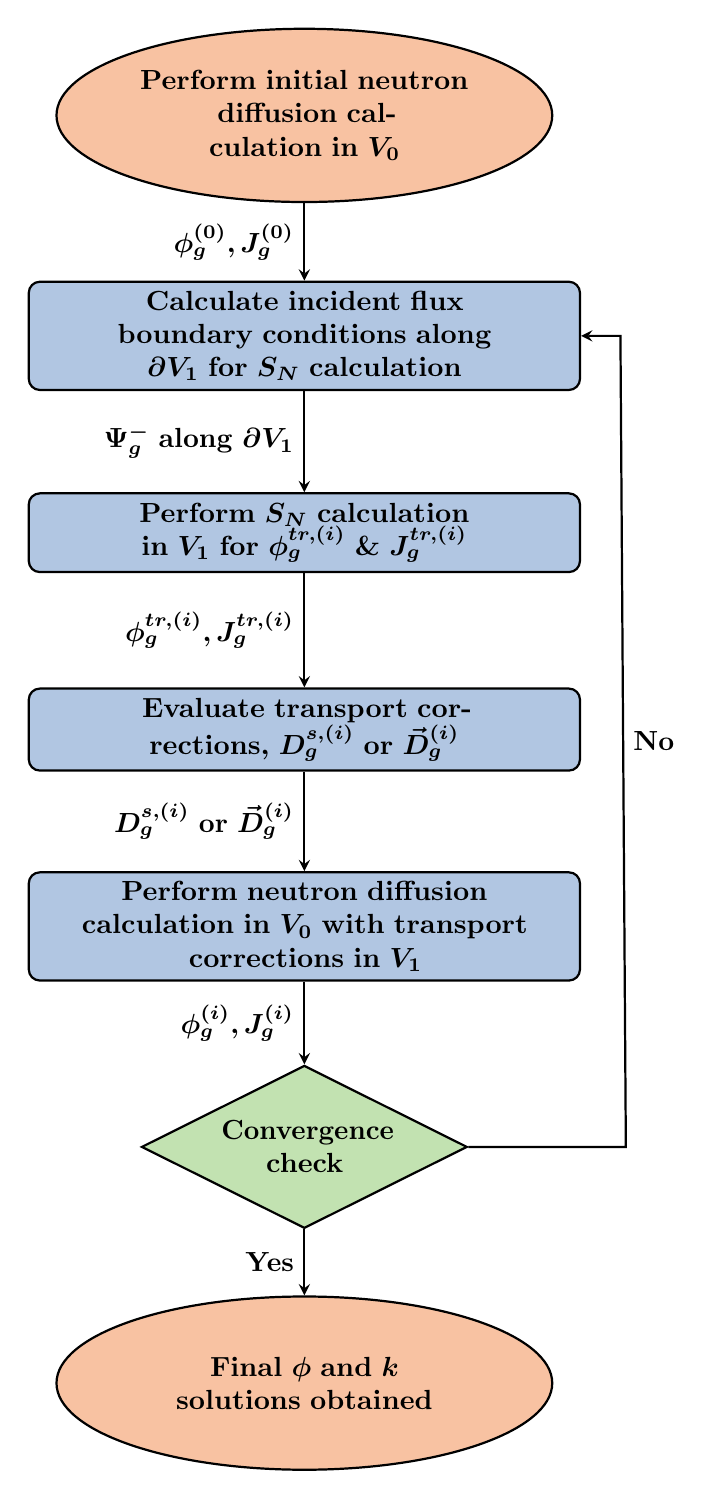
\begin{tikzpicture}
    \node (1) [object] {\textbf{Perform initial neutron\\diffusion calculation in $\bm{V_0}$}};
    \node (2) [process, below of=1, yshift=-1.8cm]
      {\textbf{Calculate incident flux boundary conditions along\\$\bm{\partial V_1}$ for $\bm{S_N}$ calculation}};
    \node (3) [process, below of=2, yshift=-1.5cm]
      {\textbf{Perform $\bm{S_N}$ calculation\\in $\bm{V_1}$ for $\bm{\phi^{tr,(i)}_g}$ \& $\bm{J^{tr,(i)}_g}$}};
    \node (4) [process, below of=3, yshift=-1.5cm]
      {\textbf{Evaluate transport corrections, $\bm{D^{s,(i)}_g}$ or $\bm{\vec{D}^{(i)}_g}$}};
    \node (5) [process, below of=4, yshift = -1.5cm]
      {\textbf{Perform neutron diffusion\\calculation in $\bm{V_0}$ with transport\\corrections in $\bm{V_1}$}};
    \node (6) [decision, below of=5, yshift = -1.8cm]
      {\textbf{Convergence\\check}};
    \node (7) [object, below of=6, yshift = -2cm]
      {\textbf{Final $\bm{\phi}$ and $\bm{k}$\\solutions obtained}};
    \draw [arrow] (1) -- node[anchor=east] {$\bm{\phi^{(0)}_g, J^{(0)}_g}$} (2);
    \draw [arrow] (2) -- node[anchor=east] {$\bm{\Psi^-_g}$ \textbf{along} $\bm{\partial V_1}$} (3);
    \draw [arrow] (3) -- node[anchor=east] {$\bm{\phi^{tr,(i)}_g, J^{tr,(i)}_g}$} (4);
    \draw [arrow] (4) -- node[anchor=east] {$\bm{D^{s,(i)}_g}$ \textbf{or} $\bm{\vec{D}^{(i)}_g}$} (5);
    \draw [arrow] (5) -- node[anchor=east] {$\bm{\phi^{(i)}_g, J^{(i)}_g}$} (6);
    \draw [arrow] (6) -- node[anchor=east] {\textbf{Yes}} (7);
    \draw [arrow] (6) -- ([shift={(2cm,0cm)}]6.east)-- node[anchor=west] {\textbf{No}} ([shift={(0.5cm,0cm)}]2.east)--(2);
  \end{tikzpicture}
  \caption{Algorithm flowchart for the hybrid $S_N$-diffusion method. $(i)$ denotes the iteration
  index.}
  \label{fig:algorithm}
\end{figure}

\section{$S_N$ Subsolver Boundary Conditions} \label{sec:sn-bc}

For the hybrid $S_N$-diffusion method to converge, it requires appropriate boundary conditions for
the $S_N$ subproblem.
Given that we want to limit the coverage of $V_1$ to the control rod region and its
immediate vicinity, $V_1$ should be sufficiently smaller than $V_0$, but large enough to capture
anisotropies in the flux due to the control rod. As a consequence, the boundaries $\partial V_1$ 
lie well within $V_0$. Crucially, there is no feasible method of generating
accurate boundary fluxes for an $S_N$ solver from a neutron diffusion flux solution. We may obtain
the best estimate by applying the $P_1$ approximation for evaluating the neutron angular flux along
the discrete ordinates $\hat{\Omega}_d$ of the $S_N$ angular quadrature set as follows
%
\begin{align}
  \Psi_{g,d} &\approx \frac{1}{4\pi}\left(\phi^\text{diff}_g+3\hat{\Omega}_d\cdot
  \vec{J}^\text{diff}_g\right) \nonumber \\
  &=\frac{1}{4\pi}\left(\phi^\text{diff}_g-3\hat{\Omega}_d\cdot D_g\nabla\phi^\text{diff}_g\right)
\end{align}
%
where the diff superscript denotes flux estimates from the latest neutron diffusion calculation.
With this relation, we can formulate the boundary source term for the $S_N$ subsolver by setting
$\Psi^\text{inc}_{g,d}$ in Eq.\ \ref{eq:boundary-source} to
%
\begin{gather}
  \Psi^\text{inc}_{g,d} = \frac{1}{w}
  \left(\phi^\text{diff}_g-3\hat{\Omega}_d\cdot D_g\nabla\phi^\text{diff}_g\right)
\end{gather}

\section{Buffer Region} \label{sec:buffer-region}

The $S_N$ subsolver boundary conditions will generally cause deviations
in the flux and transport correction values since the $P_1$ approximation is accurate for up to
linear anisotropies in the flux. However, as I will show in Chapter \ref{chap:msre},
the influence of boundary conditions on the accuracy of
the transport correction terms does not extend far from the boundary $\partial V_1$ in optically
thick media due to competing influences from the bulk scattering and absorption effects in $V_1$.
Results in Chapter \ref{chap:msre} will show that transport correction values
($D^s_g$ or $\vec{D}_g$) generated with the $S_N$ subsolver within $V_1$ are accurate everywhere up
to a few centimeters away from $\partial V_1$.

For accurate flux estimates with the hybrid method, I propose that $V_1$ must be large enough to
provide accurate transport corrections near the highly-absorbing control rod while simultaneously
accommodating for inaccurate transport correction values near $\partial V_1$. Right before each
neutron diffusion calculation, the solver must determine where the inaccurate transport correction
values occur and discard them. I will refer to the region near $\partial V_1$ in which the
transport correction values are discarded as the \textit{buffer region} ($V_1'$).
$V_1'$ shares the same outer boundary $\partial V_1$ as $V_1$. Consequently, the neutron
diffusion calculation on $V_0$ will only apply transport corrections in $V_1$ excluding $V_1'$.

In this discussion thus far, I have yet to establish the cutoff boundary for $V_1'$ within $V_1$
opposite to $\partial V_1$. A natural/intuitive criterion for the location of the cutoff boundary
would be wherever the components of the drift correction variable $\vec{D}_g$ is zero, i.e.,
wherever the components change signs. The reasons for this criterion are twofold. Firstly, at
points where the $\vec{D}_g$ components are zero, the flux is approximately isotropic along the
axes corresponding to the components because value of $\vec{D}_g$ represents how much correction a
standard neutron diffusion model requires. Secondly, this choice preserves the smoothness of the
neutron flux and flux gradient.
%
\begin{figure}[htb!]
	\centering
	\includegraphics[width=.75\columnwidth]{case-3b-geometry}
	\caption{1-D geometry for Case 3b.}
	\label{fig:3b-geometry}
\end{figure}

Here, I use Case 3b of the 1-D test cases to be covered in Chapter \ref{chap:msre}
to illustrate the buffer region and the behavior of $\vec{D}_g$. Case 3b is a 1-D slab problem
consisting of control rod, air, fuel-graphite repeating lattice, and reactor vessel regions as
shown in Figure \ref{fig:3b-geometry}. The fuel regions are neutron-multiplying media containing
$^\text{235}$U fissile material. I took material compositions of each region from the \gls{MSRE}
reference design and the start-up fuel composition \cite{fratoni_molten_2020}.
Case 3b has reflecting boundary conditions on the left boundary and vacuum boundary conditions on
the right boundary.
%
\begin{figure}[htb!]
    \centering
    \begin{subfigure}[t]{.49\textwidth}
        \centering
        \includegraphics[width=\textwidth]{case-3b-group-1-drift}
    \end{subfigure}
    \hfill
    \begin{subfigure}[t]{.49\textwidth}
        \centering
        \includegraphics[width=\textwidth]{case-3b-group-8-drift}
    \end{subfigure}
    \caption{The reference and hybrid drift ($\vec{D}_g$) distributions for group 1 and 8 calculated
      from $S_8$ and $S_8$-diffusion simulations. The correction subregion $V_1$ spans $x=0$ cm to
      $x=10$ cm.}
    \label{fig:3b-drift}
\end{figure}

I ran an eight energy group $S_8$ $k$-eigenvalue simulation with the newly implemented $S_N$ solver
on Moltres to generate reference $\vec{D}_g$ distributions. I also ran an eight-group hybrid
$S_8$-diffusion simulation with the $S_8$ method for generating $\vec{D}_g$ in $V_1$. I set $V_1$
to encompass the control rod region and its vicinity from $x=0$ to $10$ cm based on the geometry in
Figure \ref{fig:3b-geometry}. Figure \ref{fig:3b-drift} shows the $\vec{D}_1$ and $\vec{D}_8$
distributions from $x=0$ to $15$ from the reference $S_8$ and hybrid simulations. The hybrid
$\vec{D}_g$ distribution is zero beyond $x=10$ cm because no corrections are generated outside of
$V_1$. Comparing the hybrid distributions to the reference distributions in both energy groups, the
hybrid distributions are accurate up to around $x=8$ cm. Working backward towards the control rod
at $x=0$-$0.5$ cm, the $\vec{D}_g$ values go to zero at $x=7.5$ cm. Therefore, the buffer
region $V_1'$ lies between $x=7.5$ cm and $x=10$ cm. While $V_1$ is pre-determined at the start of
the simulation and fixed for all energy groups, $V_1'$ does not necessarily coincide for all
energy groups and coordinate axes.

\section{Numerical Implementation}

In this section, I detail the numerical implementation of the hybrid $S_N$-diffusion method with
drift correction terms. As mentioned in Section \ref{sec:transport-correction}, I opted for the
drift correction terms over diffusion correction for investigations beyond 1-D test cases.
Therefore, for brevity, I moved numerical implementation details for the hybrid method with
diffusion correction to Appendix A.

In Section \ref{sec:moltres-description}, I detailed the code structure of Moltres
\cite{lindsay_moltres_2017} in relation to the underlying \gls{MOOSE} finite-element framework
\cite{giudicelli_30_2024} and the pre-existing multigroup neutron diffusion and thermal-hydraulics
models. I implemented the hybrid $S_N$-diffusion model in Moltres to
leverage existing capabilities and functions that are also relevant to the new $S_N$ neutron
transport model and the $S_N$-to-diffusion coupling features. I also leveraged several basic
functions from \gls{MOOSE} that are useful for setting up physics models.

All source code for the hybrid $S_N$-diffusion model is hosted on my Moltres GitHub fork
repository\footnote{\url{https://github.com/smpark7/moltres/tree/sn-method}} as of the time of
writing. This branch may be merged into the original upstream Moltres GitHub repository in the near
future.

Moltres presently comes with a Python script for parsing and extracting neutron group constant data
from OpenMC \cite{boyd_multigroup_2019} or Serpent 2 \cite{leppanen_serpent_2014} simulation
output files. The script reorganizes the group constant data into a
JSON format file. I expanded the Python script to extract
the macroscopic total cross sections $\Sigma_{t,g}$ and the higher-order macroscopic Legendre
scattering moments $\Sigma^{g'\rightarrow g}_{s,l}$ for the $S_N$ neutron transport model. A new
\texttt{Material} class called \texttt{MoltresSNMaterial} creates material
property variables for each group constant for the $S_N$ model to read during a neutronics
simulation. If the user provides group constant data at multiple reactor temperature states,
\texttt{MoltresSNMaterial} can interpolate the data to simulate temperature-dependent reactivity
changes.

The new \texttt{MoltresUtils} class contains ``utility'' functions required by the $S_N$ model.
These functions include: a function to retrieve directions and weights defined by a
level-symmetric quadrature set of order $N$, a function to retrieve reflecting directions at
reflecting boundaries, and a function to compute spherical harmonic flux moments for anisotropic
scattering. I pre-computed the direction and weight values for the level-symmetric quadrature sets
using a Python script and hard-coded them in Moltres to reduce computational burden during
simulations.

The \gls{SAAF} $S_N$ method defines $G$ energy groups and $N_d$ discrete directions for a total
of $G\times N_d$ angular flux variables $\Psi_{g,d}$. The Moltres $S_N$ model groups the
$\Psi_{g,d}$ variables by energy group into $G$ array variables. An array variable is a
set of standard field variables to help with dealing with setting up simulations with high
dimensionality. Each standard variable of an array variable is referred to as a component in the
array variable. In this work, I opted for
2nd-order Lagrange shape functions to approximate the $\Psi_{g,d}$ variables in the finite-element
analysis. The 2nd-order approximation showed better convergence rates in mesh refinement studies.

The terms in the \gls{SAAF} $S_N$ equations (Eqs.\ \ref{eq:time-derivative}-\ref{eq:reflecting-bc})
are represented by kernel and BC classes inheriting from \texttt{ArrayKernel} and
\texttt{ArrayIntegratedBC} template classes. Table \ref{tab:saaf-sn} lists the class names
corresponding to each term in Eq.\ \ref{eq:saaf-vt}.
%
\begin{table}[htb]
  \centering
  \caption{Names of the Kernels and BCs representing the \gls{SAAF} $S_N$ equations.}
  \begin{tabular}{l l l}
    \toprule
    Term name & Class name \\
    \midrule
    Time derivative & \texttt{SNTimeDerivative} \\
    Streaming & \texttt{SNStreaming} \\
    Collision & \texttt{SNCollision} \\
    Scattering & \texttt{SNScattering} \\
    Prompt fission source & \texttt{SNFission} \\
    Delayed neutron source & \texttt{SNDelayed} \\
    Vacuum boundary & \texttt{SNVacuumBC} \\
    Reflecting boundary & \texttt{SNReflectingBC} \\
    Hybrid method boundary source & \texttt{SNDiffusionBC} \\
    \bottomrule
  \end{tabular}
  \label{tab:saaf-sn}
\end{table}

The \gls{MOOSE} framework leverages the Eigen \cite{guennebaud_eigen_2010} C++ template library for
linear algebra operations defined in ArrayKernels and ArrayBCs for array variables. The \gls{SAAF}
$S_N$ kernels and BCs contain functions for computing the residual and Jacobian contributions of
each term. The \gls{FEM} numerical solver deems to have reached a converged solution if the sum of
residual contributions falls below a defined tolerance value. All $S_N$ simulations in this work
employ the \gls{PJFNK} method \cite{knoll_jacobian-free_2004} with HYPRE-BoomerAMG
\cite{hypre_hypre_2022} for preconditioning. BoomerAMG is a parallel implementation of the
algebraic multigrid method from the HYPRE linear solver library.

Moltres initializes the drift correction variables $\vec{D}_g$ as auxiliary array variables
with three components corresponding to their $x$, $y$, and $z$ components. Auxiliary variables
encompass all field variables which are not directly determined during the \gls{PJFNK}
calculation stage. The drift and boundary correction variables are computed during the
post-calculation stages using $\Psi_{g,d}$.
I created new kernel classes, \texttt{GroupDrift} and \texttt{VacuumCorrectionBC}, to add the
drift and boundary correction terms to the transport-corrected neutron diffusion solver.

I employed the \texttt{MultiApp} system \cite{gaston_physics-based_2015} to implement the fixed point
iterative coupling between the $S_N$ and neutron diffusion solvers for the hybrid $S_N$-diffusion method.
The \texttt{MultiApp} and \texttt{Transfers} systems from \gls{MOOSE} provide flexible interfaces
for setting up iterative solvers and transferring data between the solvers. A typical hybrid
method simulation on Moltres starts with the neutron diffusion solver for the first estimate of the
neutron flux distribution. Moltres transfers the neutron flux distribution to the $S_N$ solver to
compute the boundary source distribution. The $S_N$ solver then generates its own flux estimate and
computes drift and boundary correction variables for the neutron diffusion solver. Moltres
transfers the correction variables to the neutron diffusion solver to compute its next flux
estimate. This process iterates until the neutron flux distribution converges to within tolerance
values provided in the input file.

\section{Summary} \label{sec:hybrid-summary}

The hybrid $S_N$-diffusion method improves on the standard neutron
diffusion method by iteratively applying transport corrections generated from solving the $S_N$
neutron transport
method in subdomains containing highly neutron-absorbing regions (e.g., control rods). By limiting
the size of the subdomain in which $S_N$ subsolver is active, the hybrid method saves on
computational expense at the cost of some accuracy in the regions not treated with transport
corrections. In turn, the neutron diffusion subsolver provides approximate boundary source terms
for the $S_N$ subsolver boundary conditions. 

I presented two different formulations of transport correction that I investigated in this work for
implementation in the hybrid method: diffusion correction and drift correction. Diffusion
correction involves replacing the diffusion coefficient in the neutron diffusion equations with
corrected coefficients derived from neutron transport methods. Drift correction involves
introducing additional drift terms to the neutron diffusion equations to provide transport
corrections. I found drift correction to be more promising due to issues with division by zero when
obtaining diffusion corrections.

In my investigations with the hybrid method, I found that the $S_N$ subsolver produces
accurate transport correction values in most of the subdomain. However, the transport correction
values near the $S_N$ subsolver boundary are inaccurate due to the approximate boundary conditions
provided by the diffusion subsolver. Thus, I developed and presented a numerical fix for discarding
inaccurate transport correction values and preserving the smoothness of the neutron flux and flux
gradient solution.

By implementing the hybrid method in Moltres, I leveraged existing neutronics modelling
capabilities and parallel numerical solver libraries available through Moltres and \gls{MOOSE} to
enable full-core, time-dependent reactor simulations on \gls{HPC} clusters.
In the next chapter, I verify the hybrid method against Monte Carlo and $S_N$ neutron transport
methods through various neutronics test cases and discuss some significant observations made in my
investigations.

\glsresetall

\chapter{MSRE Model \& Results}
\label{chap:msre}
Chapter \ref{chap:hybrid} laid out the mathematical background and numerical implementation
of the hybrid $S_N$-diffusion method for improving neutronic accuracy in reactor systems containing
highly neutron-absorbing regions. Chapter \ref{chap:hybrid} specifically discussed two transport
correction schemes for the hybrid method: the diffusion and drift correction
schemes. This chapter demonstrates the hybrid method through 1-D, 2-D, and 3-D $k$-eigenvalue
simulations of the \gls{MSRE}. The work in this chapter employs the OpenMC Monte Carlo neutral
particle transport software \cite{romano_openmc:_2015} to generate group constants for the hybrid
method and to generate reference solutions for method verification.
The 1-D models serve to verify the newly-implemented $S_N$ and hybrid methods
and to analyze the impact of key input parameters on the hybrid method. The
2-D models test the hybrid method performance through increased spatial dimensionality and
geometric asymmetry relative to the 1-D models. Parametric studies using 2-D models on the $S_N$ angular
discretization reveal its impact on the neutron flux distributions and $k_\text{eff}$.
Lastly, the 3-D models serve as neutronics model
validation against the \gls{MSRE} benchmark model by Fratoni et al.\ \cite{fratoni_molten_2020}.
This chapter also investigates the computational performance of 3-D simulations on a \gls{HPC}
cluster.

Section \ref{sec:msre-gc} details the OpenMC model setup for group constant generation. Section
\ref{sec:nts-methods} describes and labels the different neutronics methods employed for the
$k$-eigenvalue simulations. Section \ref{sec:test-metrics} details test metrics relevant to
neutronics verification and validation. Sections \ref{sec:1d-results}, \ref{sec:2d-results}, and
\ref{sec:3d-results} discuss the model setups, results, and discussions for the 1-D, 2-D, and 3-D
\gls{MSRE} models, respectively.

\section{Group Constant Data Generation on OpenMC} \label{sec:msre-gc}

Deterministic neutron diffusion and $S_N$ neutron transport methods require group constant data in
the form of group-averaged macroscopic neutron cross sections, neutron speeds, and delayed neutron
precursor data.
Group constants relevant to the neutron diffusion, $S_N$ neutron transport, or both
methods in Moltres are:
%
\begin{align*}
  \Sigma_{t,g}=& \mbox{ Macroscopic total cross section in group $g$,} &\\
  \Sigma_{r,g}=& \mbox{ Macroscopic removal cross section in group $g$,} &\\
  \Sigma_s^{g'\rightarrow g}=& \mbox{ Macroscopic group-to-group scattering cross section matrix,} &\\
  \Sigma_{s,l}^{g'\rightarrow g}=& \mbox{ $l$-th Legendre moment of the macroscopic
        group-to-group scattering} & \\
                           & \mbox{cross section matrix,} &\\
  \Sigma_{sp,l}^{g'\rightarrow g}=& \mbox{ $l$-th Legendre moment of the macroscopic
  group-to-group scattering production} & \\
                                        & \mbox{cross section matrix,} &\\
  D_g=& \mbox{ $P_1$-based diffusion coefficient in group $g$,} &\\
  \nu\Sigma_{f,g}=& \mbox{ Product of the average number of neutrons produced per fission and} &\\
                  &\mbox{the macroscopic fission cross section in group $g$,}&\\
  \chi_g=& \mbox{ Neutron fission spectrum in group $g$.}&\\
\end{align*}

OpenMC generates these group constants using its multigroup cross section generation capability
\cite{boyd_multigroup_2019}. A group constant postprocessing script for Moltres
(\texttt{moltres\_xs.py}) parses OpenMC simulation output files and rewrites the group constant
data into a JSON format file suitable for Moltres simulations. While OpenMC provides most of the
group constants directly, the postprocessing script calculates $\Sigma_{r,g}$ as
%
\begin{align}
  \Sigma_{r,g} =& \sum^G_{g'\neq g}\Sigma_s^{g\rightarrow g'}+\Sigma_{a,g}-\left(\Sigma_{sp}^{g
    \rightarrow g} - \Sigma_s^{g\rightarrow g}\right)
  \shortintertext{where}
      \Sigma_{a,g} =& \mbox{ macroscopic absorption cross section in group $g$,} \nonumber \\
      \Sigma_{sp}^{g\rightarrow g} =& \mbox{ macroscopic scattering production cross section from
      group $g$ to $g$.} \nonumber
\end{align}
%
$\Sigma_{r,g}$ primarily represents the loss of neutrons from group $g$ through outscattering and
absorption. $\Sigma_{sp}^{g\rightarrow g}$ incorporates neutron multiplication effects from neutron
knockout reactions into the scattering cross section. Neutronics codes commonly identify neutron
knockout reactions as scattering reactions, but $\Sigma_{r,g}$ is a convenient parameter in which
to incorporate neutron knockout effects in the neutron diffusion method.
All simulations in this thesis used 2nd-order-accurate scattering cross sections approximated using
Legendre polynomials.

OpenMC uses the $P_1$ flux-limited formulation \cite{pomraning_flux-limited_1984} by default for
calculating $D_g$ as follows
%
\begin{align}
  D_g =& \frac{1}{3\Sigma_{tr,g}},
  \shortintertext{where}
  \Sigma_{tr,g} =& \frac{\langle\Sigma_{t,g}\phi_g\rangle-\langle\Sigma_{s1,g}\phi_g\rangle}
  {\langle\phi_g\rangle}, \nonumber \\
  \langle\Sigma_{t,g}\phi_g\rangle =& \int_{r\in V}dr \int_{4\pi}d\Omega\int^{E_{g-1}}_{E_g}dE\
  \Sigma_{t,g}(r,E)\Psi(r,E,\Omega), \nonumber \\
  \langle\Sigma_{s1,g}\phi_g\rangle =& \int_{r\in V}dr \int_{4\pi}d\Omega\int^{E_{g-1}}_{E_g}dE
  \int_{4\pi}d\Omega'\int^{\infty}_0dE'\int^1_{-1}d\mu\ \mu\Sigma_s(r,E'\rightarrow E,\Omega'\cdot
  \Omega)\phi(r,E',\Omega'), \nonumber \\
  \langle \phi \rangle =& \int_{r\in V}dr\int_{4\pi}d\Omega\int^{E_{g-1}}_{E_g}dE\ \Psi(r,E,\Omega)
  .\nonumber
\end{align}

All \gls{MSRE} neutronics simulations ran with the eight neutron energy group structure proposed
by Jaradat for \gls{MSRE} analysis \cite{jaradat_development_2021-1}.
Table \ref{table:energy-group} shows the upper neutron energy bounds of the eight-group structure.
This structure balances accuracy and computational expense most appropriately for this work when
compared to other various group structures investigated by Jaradat ranging from four to sixteen
groups.

\begin{table}[htb]
  \centering
  \caption{Neutron energy group structure in this work. Originally devised by Jaradat
  \cite{jaradat_development_2021-1}.}
  \begin{tabular}{r S}
    \toprule
    Group & {Upper energy bound [eV]} \\
    \midrule
    1 & 2.000$\times 10^7$ \\
    2 & 1.353$\times 10^6$ \\
    3 & 6.734$\times 10^4$ \\
    4 & 9.118$\times 10^3$ \\
    5 & 1.487$\times 10^2$ \\
    6 & 4.000$\times 10^0$ \\
    7 & 6.250$\times 10^{-1}$ \\
    8 & 8.000$\times 10^{-2}$ \\
    \bottomrule
  \end{tabular}
  \label{table:energy-group}
\end{table}

Material compositions and densities of all components in the \gls{MSRE} models are from reference
\gls{MSRE} specifications \cite{robertson_msre_1965, fratoni_molten_2020}.
All OpenMC simulations in this work used the ENDF/B-VII.1 nuclear data library
\cite{chadwick_endf/b-vii.1_2011}. All models have a uniform
temperature of 900 K unless otherwise stated. Sections \ref{sec:1d-model-setup},
\ref{sec:2d-model-setup}, \ref{sec:3d-model-setup} provide detailed information pertaining
specifically to the 1-D, 2-D, and 3-D model geometries, respectively.

\section{Neutronics Methods} \label{sec:nts-methods}

Besides generating group constants for the deterministic methods, OpenMC also provides reference
netruon flux and $k_\text{eff}$ values for all studied cases. OpenMC can run in continuous-energy
(OpenMC-CE) and multigroup (OpenMC-MG) modes. Table
\ref{table:var} details how OpenMC and the deterministic methods represent the position, direction
of travel, neutron energy, and angle-dependence in $\Sigma_s$. The hybrid $S_N$-diffusion method
features representations from either $S_N$ or neutron diffusion depending on the subregion under
consideration. Comparing OpenMC-MG results with OpenMC-CE results allows us
to quantify errors arising from neutron energy group discretization and the 2nd-order scattering
cross section approximations.

\begin{table}[htb!]
  \centering
  \footnotesize
  \caption{Variable representations in OpenMC under continuous-energy (OpenMC-CE) and multigroup
  (OpenMC-MG) modes, and in the $S_N$ neutron transport and neutron diffusion.}
  \begin{tabular}{l l l l l}
    \toprule
    Variable & OpenMC-CE & OpenMC-MG & $S_N$ Transport & Diffusion \\
    \midrule
    Position, $\bm{r}$ & Continuous & Continuous & Discrete & Discrete \\
    Direction of travel, $\bm{\hat{\Omega}}$ & Continuous & Continuous & Discrete & N/A \\
    Energy, $E$ & Continuous & Discrete & Discrete & Discrete \\
    Angle resolution in $\Sigma_s$ & Continuous & $L=2$ & $L=2$ & N/A \\
    \bottomrule
  \end{tabular}
  \label{table:var}
\end{table}

The rest of this section pertains to the deterministic neutronics methods used in this work for
modeling the \gls{MSRE}.
For the 1-D models, I performed neutronics calculations with the $S_N$, neutron diffusion, and
hybrid method implementations in Moltres and Python. Table \ref{table:nts-methods} highlights the
differences between the two implementations. The $S_N$ neutron transport method implementation in
Moltres follows the methodology for solving the \gls{SAAF} formulation of the $S_N$ equations as
described in Section \ref{sec:saaf} while the implementation in Python follows the methodology
for solving the original first-order formulation as described in Section \ref{sec:python-sn}.

Moltres discretizes the problem domain in space using the finite element
method while the Python implementation uses finite difference or diamond difference schemes. The
most crucial difference lies in the transport correction formulations for the hybrid method. The
Moltres implementation uses the drift correction scheme described in Section
\ref{sec:drift-correction} while the Python implementation uses the diffusion correction
scheme described in Section \ref{sec:diffusion-correction}.

This chapter refers to the methods and results from the Moltres and Python implementations
with the Moltres- or Python- prefix, i.e., Moltres-$S_N$, Moltres-diffusion, Moltres-hybrid,
Python-$S_N$, Python-diffusion, and Python-hybrid.

For 2- and 3-D models, the diffusion correction formulation is abandoned in favor of the drift
correction formulation due to superior numerical performance in the latter. Readers may find the
analysis supporting this decision in the analysis of 1-D results in Section \ref{sec:1d-results}.

\begin{table}[htb!]
  \centering
  \footnotesize
  \caption{Implementation differences of neutronics methods on Moltres and Python.}
  \begin{tabular}{l l l}
    \toprule
    Implementation detail & Moltres & Python \\
    \midrule
    Spatial discretization & Finite element method & Finite difference \& Diamond difference \\
    $S_N$ formulation & SAAF & First-order \\
    $S_N$ acceleration & Nonlinear diffusion acceleration & None \\
    Hybrid transport correction & Drift correction & Diffusion correction \\
    \bottomrule
  \end{tabular}
  \label{table:nts-methods}
\end{table}

\section{Test Metrics} \label{sec:test-metrics}

This section defines several metrics for comparing simulation results among the various
neutronics methods.
For steady-state eigenvalue calculations, all solvers directly provide the effective neutron
multiplication factor ($k_\text{eff}$), the rate of neutron population increase between successive
neutron generations. Reactivity is defined as
%
\begin{gather}
  \rho \equiv \frac{k_\text{eff}-1}{k_\text{eff}}.
\end{gather}
%
Differences in reactivity, for either comparisons between neutronics methods or control rod worth
calculations, can be calculated as
%
\begin{gather}
  \Delta\rho_{1,2} = \rho_1 - \rho_2 =
  \frac{k_{\text{eff},1}-k_{\text{eff},2}}{k_{\text{eff},1}k_{\text{eff},2}}.
\end{gather}

Spatially dependent variables (e.g., neutron group flux, neutron drift) are sampled at fixed 0.1 cm
intervals along the specified lines (e.g., horizontal, diagonal, etc.) regardless of the actual
mesh resolution.

\section{1-D Neutronics Models \& Results} \label{sec:1d-results}

This section presents the models, results, and discussion for the 1-D test cases. Section
\ref{sec:1d-model-setup} describes the model setup and geometries of the 1-D test cases.
Section \ref{sec:1d-mesh-conv} discusses the 1-D mesh convergence tests. Lastly, Section
\ref{sec:1d-results-sub} shows the results and discussion of the 1-D test cases.

\subsection{1-D Neutronics Model Setup \& Geometries} \label{sec:1d-model-setup}

This section covers six 1-D test cases with increasing complexity to verify the $S_N$ and hybrid
$S_N$-diffusion implementations and to test the performance of the hybrid
method in response to various geometrical features. The last two cases resemble the
reference \gls{MSRE} design \cite{robertson_msre_1965}, which has centrally located control rods
and air-filled rod guide tubes. Figure \ref{fig:case-geom} shows the geometries of Cases 1a to
3b. All geometries have reflective boundary conditions at $x=0$ cm, thereby
forming half-core or repeating unit cell models. Cases 1a and 1b are repeating unit
cell models with reflecting boundaries on the right-side boundaries. Cases 2a, 2b, 3a, and 3b
are 1-D half-core models with vacuum boundaries on the right-side boundaries.

\begin{figure}[htb!]
  \centering
  \includegraphics[width=0.8\columnwidth]{case-geometry}
  \caption{Geometries of the 1-D test cases. The material labeled ``mixture'' represents a
    homogeneous mixture of fuel and graphite at a ratio of 22.5\%-77.5\% by volume. All geometries
    have reflective boundary conditions on the boundary at $x=0$ cm. The right-side boundaries are
    reflective for Cases 1a and 1b, and vacuum for Cases 2a, 2b, 3a, and 3b.}
  \label{fig:case-geom}
\end{figure}

Cases 1a and 1b are simple test cases containing neutron multiplying regions. Cases 1a and 1b serve
to verify basic neutronics phenomena modeling (e.g., fission, scattering, absorption) of the newly
implemented $S_N$ and neutron diffusion methods in Python and $S_N$ method in Moltres. I did not
apply the hybrid method on these cases. Cases 2a and 2b represent 1-D models of the \gls{MSRE} with
air-filled control rod guide tube regions, a homogenized fuel-graphite lattice regions, and outer
vessel regions. Case 2b additionally contains a 0.5cm-thick control rod region to contrast with
Case 2a for control rod worth calculations. Cases 3a and 3b retain the heterogeneous fuel-graphite
lattice geometry present in the \gls{MSRE}.

In preliminary investigations, the original control rod material composition
(70 wt\% Gd$_2$O$_3$-30 wt\% Al$_2$O$_3$) led to excessively large control rod worth estimates of
approximately 55000 pcm in the 1-D models, effectively halving the $k_\text{eff}$. The worth
estimates are ten times larger
than the 5500 pcm expected from full rod insertion of all three rods in the actual \gls{MSRE}
\cite{fratoni_molten_2020}. Therefore, the proportion of Gd$_2$O$_3$ was reduced to 0.35 wt\% for a
fairer assessment of rod worth in the 1-D models. This change
brought the new rod worth estimates down to below 20000 pcm.

\subsection{1-D Neutronics Model Mesh Convergence Tests} \label{sec:1d-mesh-conv}

This mesh convergence tests were run on Case 3b for the neutron diffusion and $S_N$ neutron
transport methods. Table \ref{table:mesh-size} shows the mesh element sizes at mesh refinement
level 0. Mesh element sizes approximately halve with each successive refinement level up to level 4.

\begin{table}[t]
  \centering
  \caption{Mesh element sizes at mesh refinement level 0.}
  \begin{tabular}{l S}
    \toprule
    Region & {Mesh size [cm]} \\
    \midrule
    Control rod (interior) & 0.04 \\
    Control rod (near interface) & 0.025 \\
    Air & 0.125 \\
    Fuel & 0.1875 \\
    Graphite & 0.19375 \\
    Vessel & 0.2 \\
    \bottomrule
  \end{tabular}
  \label{table:mesh-size}
\end{table}

\begin{figure}[t]
  \centering
  \begin{subfigure}[b]{0.48\columnwidth}
    \centering
    \includegraphics[width=\columnwidth]{diffusion-mesh-convergence-k}
    \caption{Neutron diffusion method}
    \label{fig:diff-mesh-k}
  \end{subfigure}
  \hfill
  \begin{subfigure}[b]{0.48\columnwidth}
    \centering
    \includegraphics[width=\columnwidth]{sn-mesh-convergence-k}
    \caption{$S_8$ neutron transport method}
    \label{fig:sn-mesh-k}
  \end{subfigure}
  \caption{Convergence of multiplication factor ($k_\text{eff}$) estimates for Case 3b across four
    levels of mesh refinement relative to the finest mesh resolution.}
  \label{fig:mesh-k}
\end{figure}

Figures \ref{fig:diff-mesh-k} and \ref{fig:sn-mesh-k} show the convergence of $k_\text{eff}$
estimates observed for Case 3b simulations with neutron diffusion and $S_8$ neutron transport
methods. The $k_\text{eff}$ values plateau at 0.97132 and 0.98138 for the neutron diffusion and
$S_8$ methods, respectively. After two rounds of mesh refinements, both methods fall within
$5\times 10^{-7}$ range of the reference $k_\text{eff}$ values, below the 0.1 pcm ($10^{-5}$)
threshold for determining solution convergence.

Figures \ref{fig:diff-mesh-flux} and \ref{fig:sn-mesh-flux} show the absolute differences in the
group flux distributions at mesh refinement levels 1 to 3 relative to the reference group flux
distribution at level 4 (maximum refinement). The plots omit data from level 0 to improve the fidelity
of the plots as flux differences drop significantly by one order of magnitude with each level of
refinement.
These results show that the mesh resolution at level 2 is a sufficient guideline for
the mesh resolutions used in the subsequent 1-D analyses. Given that the hybrid $S_N$-diffusion
method comprises of a combination of those
methods, the hybrid simulations were fully spatially resolved on meshes that are
appropriately resolved for both neutron diffusion and $S_N$ simulations.

\begin{figure}[htb!]
  \centering
  \includegraphics[width=.96\columnwidth]{diffusion-mesh-convergence-flux}
  \caption{Absolute difference in group fluxes ($\phi_g$) from the neutron diffusion method for
  mesh refinement levels 1 to 3 relative to the reference group flux distributions at mesh
  refinement level 4. Flux differences fall by an order of magnitude with each successive mesh
  refinement.}
  \label{fig:diff-mesh-flux}
\end{figure}

\begin{figure}[htb!]
  \centering
  \includegraphics[width=.96\columnwidth]{sn-mesh-convergence-flux}
  \caption{Absolute difference in group fluxes ($\phi_g$) from the $S_8$ neutron transport method
  for mesh refinement levels 1 to 3 relative to the reference group flux distributions at mesh
  refinement level 4. Flux differences fall by an order of magnitude with each successive mesh
  refinement.}
  \label{fig:sn-mesh-flux}
\end{figure}

\FloatBarrier

\subsection{1-D Neutronics Numerical Results \& Discussion} \label{sec:1d-results-sub}

\subsubsection{Reactivity}

Figure \ref{fig:1d-rho} shows the difference in reactivities of OpenMC-MG, $S_8$,
neutron diffusion, and hybrid methods relative to OpenMC-CE. The standard deviations of
reactivity values from OpenMC-CE are approximately 40 pcm for Cases 1a and 1b and 60 pcm for the
rest as depicted by the blue highlighted area in Figure \ref{fig:1d-rho}. For Cases 1a and 1b, the
OpenMC-MG, $S_8$, and neutron diffusion methods show excellent agreement with OpenMC-CE as the
reactivity values fall within the one or two standard deviation range. The Case 1 results show
the Moltres and Python implementations are consistent with each other given that they are spatially
well-resolved.

\begin{figure}[htb!]
  \centering
  \includegraphics[width=\columnwidth]{rho}
  \caption{Difference in reactivity $\rho$ of all neutronics methods investigated relative
  to OpenMC-CE. The standard deviation refers to the uncertainty associated with the Monte Carlo
  method in OpenMC-CE.}
  \label{fig:1d-rho}
\end{figure}

For all cases, the OpenMC-MG and the $S_8$ methods show consistent agreement with one another. 
While they deviate from OpenMC-CE by approximately 350 pcm for Cases 2a and 3a, they fall within
two standard deviations of OpenMC-CE for Cases 2b and 3b. When increasing the maximum Legendre
polynomial order to approximate the angular dependence in $\Sigma_s^{g'\rightarrow g}$ from
2nd-order to 3rd-order, the reactivity changed by only 1 pcm. Therefore, I attribute the reactivity
discrepancies to the eight neutron energy group structure which remains the
only significant difference between OpenMC-CE and the multigroup methods.

The neutron diffusion and hybrid methods agree closely with one another for Cases 2a and 3a which
exclude the control rod region. This shows that the hybrid method provides similar $k_\text{eff}$
estimates to the neutron diffusion method in 1-D simulations without highly neutron-absorbing
regions. Compared to the OpenMC-MG and $S_8$ reactivity values, the neutron diffusion and hybrid
method reactivity values agree closer with the reference OpenMC-CE value. However, this is likely
due to favorable error cancellation in these lower-fidelity methods. Figures \ref{fig:3a-flux} and
\ref{fig:3a-flux-diff} show OpenMC-MG and the $S_8$ methods reproduce
the OpenMC-CE flux distribution more accurately than the neutron diffusion and hybrid methods.

In Cases 2b and 3b, the neutron diffusion method largely fails to accurately capture the
effect of introducing the control rod region as evidenced by the -1500 pcm and -1150 pcm
discrepancies relative to OpenMC-CE. The hybrid method fares better with -400 pcm and -300 pcm
discrepancies.

\subsubsection{Control rod worth}

Moving the discussion to control rod worths, figure \ref{fig:1d-worth} shows the percentage
difference in rod worths for Cases 2 and 3 of OpenMC-MG, $S_8$, neutron diffusion, and hybrid
methods relative to OpenMC-CE. I calculated the rod worth estimates from each method by taking the
difference in reactivity between the ``rod out'' (a) and ``rod in'' (b) configurations of Cases 2
and 3. All neutronics methods overestimate the rod worth relative to OpenMC-CE, resulting in
positive percentage difference values observed in the figure.
The neutron diffusion methods clearly show up as outliers with rod worth estimates in excess
of 8\%. Most of the remaining methods cluster around 2.5\% and 3\% percentage difference for Cases
2 and 3 with the exception of the Python-hybrid method for Case 3 reporting a 1.5\% difference.
The diffusion correction scheme in Python deviates from the drift correction
scheme in Moltres due to numerical issues with division by zero around flux maximas and minimas
in the fuel-graphite lattice region.

Given that the hybrid methods rely on transport corrections derived from the $S_N$ method, the
$S_8$ rod worth estimates serve as the
reference point for hybrid method verification. Additionally, errors arising from the multigroup
approximation affect both hybrid and $S_N$ simulations to similar degrees. While the Python-hybrid
method produces the lowest percentage difference relative to OpenMC-CE for Case 3, the
Python-hybrid method deviates from the $S_8$ ``multigroup'' reference rod worths more than the
Moltres-hybrid method. Nevertheless, both hybrid method implementations provide significant
improvements in rod worth estimates over the neutron diffusion method.

\begin{figure}[h]
  \centering
  \includegraphics[width=\columnwidth]{worth}
  \caption{Percentage difference in rod worth for Cases 2 and 3 of all neutronics methods
  investigated relative to OpenMC-CE. All percentage difference values are consistently positive.}
  \label{fig:1d-worth}
\end{figure}

\subsubsection{Neutron flux distribution}

This discussion on the neutron flux distributions focuses on Cases 3a and 3b which most closely
resemble the actual \gls{MSRE} reactor geometry. Cases 3a and 3b resemble the \gls{MSRE} reactor
with a control rod withdrawn and inserted, respectively. Figures \ref{fig:3a-flux} and
\ref{fig:3b-flux} show the neutron group flux distributions for Cases 3a and 3b from OpenMC-CE and
OpenMC-MG. Differences between the two methods arise from the multigroup approximation, notably in
group 2 for Case 3a and groups 2, 6, 7, 8 for Case 3b. Future work aimed at finding a better
neutron energy group structure should at minimum focus on improving fidelity in the listed energy
groups.

For a fair evaluation of the deterministic multigroup methods without distortions from the
multigroup approximation, I chose to compare their flux distributions with the OpenMC-MG flux
distribution. Figures \ref{fig:3a-flux-diff} and \ref{fig:3b-flux-diff} show the absolute
difference in neutron group flux distributions of the Moltres-$S_8$, Moltres-diffusion,
Moltres-hybrid, and Python-hybrid methods relative to OpenMC-MG. The figures omit Python-$S_8$ and
Python-diffusion as their distributions are nearly identical to their Moltres-based counterparts.
The neutron diffusion and hybrid methods fare worse than the $S_8$ method at capturing the
oscillatory pattern in groups 1, 2, 5, 7, and 8 arising from the fuel-graphite lattice geometry
along $x=5$ cm to 10 cm. In both Cases 3a and 3b, the neutron diffusion method (yellow plot lines)
exhibits significant flux deviations in groups 1, 2, 7, and 8 near $x=0$ cm.

Both hybrid methods
provide significant improvements in neutron flux distributions compared to the neutron diffusion
method as shown by the generally smaller per-group flux deviations particularly near $x=0$ cm. The
figures also show Moltres-hybrid (green) provides more accurate flux estimates than
Python-hybrid (red) in all instances. The differences indicate deficiencies in the diffusion
correction scheme in Python-hybrid which lead to poorer performance compared to the drift
correction scheme in Moltres-hybrid.

\begin{figure}[p]
  \centering
  \includegraphics[width=\columnwidth]{case-3a-flux}
  \caption{Case 3a neutron group flux distributions from OpenMC-CE and OpenMC-MG.}
  \label{fig:3a-flux}
\end{figure}

\begin{figure}[p]
  \centering
  \includegraphics[width=\columnwidth]{case-3b-flux}
  \caption{Case 3b neutron group flux distributions from OpenMC-CE and OpenMC-MG.}
  \label{fig:3b-flux}
\end{figure}

\begin{figure}[p]
  \centering
  \includegraphics[width=\columnwidth]{case-3a-flux-diff}
  \caption{Absolute difference in neutron group flux distributions for Case 3a from Moltres-$S_8$,
  Moltres-diffusion, Moltres-hybrid, and Python-hybrid relative to OpenMC-MG.}
  \label{fig:3a-flux-diff}
\end{figure}

\begin{figure}[p]
  \centering
  \includegraphics[width=\columnwidth]{case-3b-flux-diff}
  \caption{Absolute difference in neutron group flux distributions for Case 3b from Moltres-$S_8$,
  Moltres-diffusion, Moltres-hybrid, and Python-hybrid relative to OpenMC-MG.}
  \label{fig:3b-flux-diff}
\end{figure}

\FloatBarrier

\subsubsection{Drift \& diffusion correction distribution}

Figures \ref{fig:3b-drift} and \ref{fig:3b-svdc} show the distributions of the drift and diffusion
correction parameters, respectively, in each neutron energy group for Case 3b. As a reminder to the
reader, the hybrid $S_N$-diffusion methods generate these correction parameters in subregions
containing highly neutron absorbing materials. I implemented the drift correction scheme for
Moltres-hybrid and the diffusion correction scheme for Python-hybrid. The hybrid methods
selectively apply the $S_N$ method to improve neutronic modeling within the subregions. I computed
the reference distributions (orange data points) in both plots from reference flux solutions of the
standard $S_8$ method.

As discussed in Section \ref{sec:buffer-region}, both sets of correction parameters generated by
the two correction schemes match their respective reference values within the correction subregion
from $x=0$ cm to 10 cm except near the subregion boundary at $x=10$ cm. Therefore, both schemes
provide improved flux estimates in the subregion compared to the neutron diffusion method.
The prior reactivity and flux distribution results indicate Moltres-hybrid is more accurate
than Python-hybrid relative to OpenMC-MG as the reference. Therefore, subsequent hybrid method
simulations in this work are solely with the hybrid method with the drift correction scheme in
Moltres.

In Figure \ref{fig:3b-drift}, the drift
correction distributions (Moltres-hybrid) for all eight energy groups are well-defined throughout
the subregion and are continuous except at material interfaces. Consequently, the drift correction
scheme provides accurate flux corrections for about 75\% of the subregion based on the buffer
region cutoff criteria which occurs around $x=7.5$ cm where most of the drift distributions are
zero (refer to Section \ref{sec:buffer-region}). By contrast, the diffusion correction
distributions in Figure \ref{fig:3b-svdc} contains numerous discontinuities tending towards
positive or negative infinity in all eight energy groups. The discontinuities arise when
computing corrected diffusion coefficients (Eq. \ref{eq:svdc}) near flux peaks and troughs
(stationary points) where the flux gradients approach zero. The location of stationary points from
the diffusion and $S_N$ calculations in the hybrid method do not necessarily coincide, resulting in
discontinuous flux gradients in the final flux solution. Discontinuities are generally unavoidable
in most problems because the fluxes typically reach local minima in control rod regions.
Furthermore, unlike negative drift coefficients, negative diffusion coefficients are unphysical.
Taking everything into consideration, the diffusion correction scheme is less accurate and more
numerically unstable than the drift correction scheme.

The subsequent discussions on the correction region size and the number of outer
iterations focus on the drift correction scheme of the hybrid method.

\begin{figure}[p]
  \centering
  \includegraphics[width=.99\columnwidth]{case-3b-drift}
  \caption{Multigroup drift correction ($\vec{D}_g$) $x$-component distributions from the
  Moltres-hybrid and Moltres-$S_8$ solvers.}
  \label{fig:3b-drift}
\end{figure}

\begin{figure}[p]
  \centering
  \includegraphics[width=.99\columnwidth]{case-3b-svdc}
  \caption{Multigroup diffusion correction ($D^s_g$) $x$-component distributions from the
    Python-hybrid and Python-$S_8$ solvers.}
  \label{fig:3b-svdc}
\end{figure}

\FloatBarrier

\subsubsection{Impact of correction subregion sizes}

The hybrid $S_N$-diffusion method relies on $S_N$ calculations in the correction subregion to
generate flux corrections. Minimizing the size of the correction subregion and the $S_N$ subproblem
is essential for the hybrid method to be computationally competitive for time-dependent full-core
simulations. I investigated the effect of the correction subregion size on the $k_\text{eff}$ and
control rod worth estimates with Cases 3a and 3b by varying the subregion sizes from 10 cm to 40 cm
at 5 cm-intervals. All subregion sizes place the subregion boundary more than 1 neutron mean free
path away from the control rod. The shortest measured neutron mean free paths are 4.81 cm and 5.85
cm for group 1 neutrons in the fuel and graphite regions, respectively.

Figures \ref{fig:v1-size-a-k} and \ref{fig:v1-size-b-k} show the $k_\text{eff}$ estimates from the
hybrid method for Cases 3a and 3b, respectively. In both cases, the $k_\text{eff}$ values initially
decrease as the correction subregion sizes increase before reversing in trend when the subregion
size reaches 35 cm and beyond. The $k_\text{eff}$ values vary by up to 164 pcm for Case 3a and 109
pcm for Case 3b. An important observation here is that the $k_\text{eff}$ values do not
monotonically converge towards the $k_\text{eff}$ estimate from the $S_8$ method. This behavior
implies that neutron leakage error remains a significant source of discrepancy as long as the
correction region does not encompass the outer boundary.

% In general,
% discrepancies arise between the neutron diffusion method and $S_8$ from the neutron diffusion 
% method's failure to accurately model the neutron flux in the fuel-graphite lattice region. The
% figures imply that those discrepancies result in a positive change in $k_\text{eff}$ since the
% $k_\text{eff}$ decreases as larger fractions of the problem domain benefit from flux corrections.
% The remaining discrepancy in $k_\text{eff}$ between the hybrid method with a correction subregion
% size of 40 cm and the $S_8$ method arises from 

\begin{figure}[htb!]
  \centering
  \begin{subfigure}[b]{0.49\columnwidth}
    \centering
    \includegraphics[width=\columnwidth]{correction-size-a-k}
    \caption{Case 3a}
    \label{fig:v1-size-a-k}
  \end{subfigure}
  \hfill
  \begin{subfigure}[b]{0.49\columnwidth}
    \centering
    \includegraphics[width=\columnwidth]{correction-size-b-k}
    \caption{Case 3b}
    \label{fig:v1-size-b-k}
  \end{subfigure}
  \caption{$k_\text{eff}$ estimates from the hybrid method for Cases 3a and 3b with different
  correction subregion sizes. The horizontal lines indicate $k_\text{eff}$ estimates from the
  OpenMC-CE, OpenMC-MG, and $S_8$ methods.}
  \label{fig:v1-size-k}
\end{figure}

Figure \ref{fig:v1-size-rho} shows the percentage difference in rod worth relative to OpenMC-CE. 
Due to the identical trends observed in the $k_\text{eff}$ estimates of both cases, the control rod
worth estimates do not change significantly when the correction subregion
sizes change. The rod worth estimates for all investigated correction subregion sizes remain within
0.2\% of the $S_8$ method. This indicates limiting the correction subregion size to save
computational cost on the expensive $S_N$ calculations has a negligible impact on rod worth
estimates.

\begin{figure}[htb!]
  \centering
  \includegraphics[width=0.8\columnwidth]{correction-size-rho}
  \caption{Percentage difference in rod worth from the hybrid method relative to OpenMC-CE for
    Cases 3a and 3b with different correction subregion sizes. The horizontal lines indicate
    equivalent rod worth differences from the OpenMC-MG and $S_8$ methods.}
  \label{fig:v1-size-rho}
\end{figure}

The $k_\text{eff}$ and rod worth results show the hybrid method is able to accurately
reproduce rod worth estimates as long as the correction subregion size remains consistent between
$k$-eigenvalue simulations used for rod worth calculations. The
correction subregion size must also be sufficiently large to capture the highly neutron-absorptive
rod's influence on the neutron flux around the rod at $x=0$ cm. The drift correction parameter
distributions in Figure \ref{fig:3b-drift} indicate that the influence of the rod on the drift, and
consequently the flux, extend to approximately $x=5$ cm before the drift distribution settles on a
regular repeating pattern influenced by the fuel-graphite lattice structure. I applied a consistent
correction subregion size of 10 cm for Cases 2 and 3 since it sufficiently meets the requirements
discussed while also minimizing the computational cost of the $S_8$ subsolver. Other reactor
designs consisting of different material components may require different minimum correction
subregion sizes.

\subsubsection{Relaxing the $S_N$ subsolver convergence threshold}

As described in Sections \ref{sec:hybrid-algorithm} \& \ref{sec:numerical-implementation}, the
hybrid $S_N$-diffusion method works by iteratively coupling a neutron diffusion solver and a $S_N$
subsolver with the latter generating drift correction parameters for the former.
The hybrid method shares some similarities with diffusion-based \gls{HOLO} acceleration schemes
(refer to Section \ref{sec:drift-correction}) for the neutron transport methods which do not
require the neutron transport side of the calculations to fully converge
\cite{reynolds_analysis_2023, wang_diffusion_2014}.
The typical convergence threshold value required for converged neutron flux calculations in Moltres
is $10^{-8}$; I set the convergence tolerance value to $10^{-8}$ for the neutron diffusion solver
and the fixed point scheme. I varied the convergence tolerance value for the $S_N$ subsolver to 
find the optimal value for maintaining sufficient solution accuracy and minimizing computational
costs; tightening the $S_N$ convergence tolerance value generally results in more outer iterations
performed before the solver meets the fixed point convergence tolerance.
Table \ref{table:sn-tol} lists the number of outer iterations required by the hybrid method for
a given set of $S_8$ subsolver convergence tolerance values in Case 3b.

\begin{table}[h]
  \centering
  \caption{Number of outer iterations in hybrid method calculations of Case 3b for a given set of
  convergence tolerance values imposed on the $S_8$ subsolver.}
  \begin{tabular}{l S S S S S S}
    \toprule
    $S_8$ subsolver tolerance, $\epsilon_\text{tol}$ & {$10^{-8}$} & {$10^{-7}$} & {$10^{-6}$} & {$10^{-5}$} & {$10^{-4}$} & {$10^{-3}$} \\
    \midrule
    Number of outer iterations & 3 & 3 & 3 & 2 & 2 & 1 \\
    \bottomrule
  \end{tabular}
  \label{table:sn-tol}
\end{table}
%
\begin{figure}[h]
  \centering
  \includegraphics[width=0.6\columnwidth]{sn-tol}
  \caption{$k_\text{eff}$ error estimates of Case 3b for a range of convergence tolerance values
  imposed on the $S_8$ subsolver relative to the reference $k_\text{eff}$ value when
  $\epsilon_\text{tol}=10^{-8}$. The $q=1.333$ line represents the approximate rate of
  convergence.}
  \label{fig:sn-tol}
\end{figure}

Figure \ref{fig:sn-tol} shows the $k_\text{eff}$ error estimates relative to the reference value
when $\epsilon_\text{tol}=10^{-8}$. The hybrid method exhibits superlinear convergence ($q=1.333$)
with respect to the $S_N$ subsolver convergence tolerance value. Based on the results, setting
$\epsilon_\text{tol}$ to $10^{-5}$ is the best balance between accuracy and computational
cost because the $k_\text{eff}$ error is less than 0.01 pcm and the number of outer iterations
would increase from 2 to 3 if the tolerance value is further tightened.

\FloatBarrier

\section{2-D Neutronics Models \& Results} \label{sec:2d-results}

This section presents the models, results, and discussion of the 2-D cases. Section
\ref{sec:2d-model-setup} describes the model setup of the 2-D cases. Section
\ref{sec:2d-nts-results} covers the results and discussion of the 2-D cases.

\subsection{2-D Neutronics Model Setup} \label{sec:2d-model-setup}

Figures \ref{fig:1/4-geom} and \ref{fig:full-geom} show the 2-D quarter-core and full-core
\gls{MSRE} models investigated. I adapted the models from the horizontal cross section of the
\gls{MSRE} numerical benchmark model \cite{fratoni_molten_2020} with the
following differences in the 2-D \gls{MSRE} model for this work:

\begin{itemize}
  \item Neglected thermal expansion of all reactor components.
  \item Modeled the control rods as perfectly annular cylinders instead of beaded control elements
    strung on flexible steel cables. Neglected the inconel shells encasing the control elements and
    the steel helical cables linking the control elements together.
  \item Set channel pitch, width, and length to 2, 0.2, and 1.2 inches, respectively.
  \item Homogenized the INOR-8 (inconel alloy reactor vessel), graphite, and molten salt regions in the sample basket.
  \item Modified the outer edge of the core graphite to be circular with no jagged edges.
  \item Replaced partial channels with full-size channels near the edge of the core graphite.
  \item Ignored the thermal insulation and shield structures outside the core.
\end{itemize}

The differences listed above, along with other changes in the 3-D model, result in negligible
changes to the $k_\text{eff}$ (refer to Section 5.6) relative to the \gls{MSRE} benchmark model
\cite{fratoni_molten_2020}.

\begin{table}[htb]
  \small
  \centering
  \setlength\tabcolsep{4pt}
  \caption{\gls{MSRE} molten salt composition when the $^{235}$U loading was at 65.25 kg.}
  \begin{tabular}{l S S S S S S S}
    \toprule
    Element & {Li} & {Be} & {Zr} & {Hf} & {$^{234}$U} & {$^{235}$U} & {$^{236}$U} \\
    \midrule
    Composition [kg] & 507.27 & 293.96 & 513.97 & 0.0029 & 0.67 & 65.25 & 0.27 \\
    \bottomrule
  \end{tabular}
  \begin{tabular}{l S S S S S S}
    \toprule
    Element & {$^{238}$U} & {Fe} & {Cr} & {Ni} & {O} & {F} \\
    \midrule
    Composition [kg] & 141.91 & 0.75 & 0.13 & 0.14 & 2.27 & 3103.22 \\
    \bottomrule
  \end{tabular}
  \label{table:2d-salt-composition}
\end{table}

INOR-8, also referred to as Hastelloy N, is a nickel-based alloy used for structural components in
the \gls{MSRE} \cite{robertson_msre_1965}.
Table \ref{table:2d-salt-composition} lists the molten salt composition for the 2-D models. The
$^{235}$U loading of 65.25 kg is the amount at which the \gls{MSRE} first achieved criticality. The
control rods consist of the original \gls{MSRE} 70 wt\% Gd$_2$O$_3$-30 wt\% Al$_2$O$_3$ mixture.
The models impose neutron vacuum boundary conditions on the outermost boundary of the INOR-8
vessel structure. The quarter-core model imposes neutron reflecting boundary conditions along the
left and bottom straight edges (Figure \ref{fig:1/4-geom}). Note that the quarter-core and
full-core models are not identical because the full-core model contains a sample basket instead of
a control rod in the lower-right segment of Figure \ref{fig:full-geom-closeup}.

I ran neutronics simulations on the quarter- and full-core models using OpenMC under both continuous
energy (OpenMC-CE) and multigroup (OpenMC-MG) modes, and using Moltres with the hybrid $S_N$-diffusion
and neutron diffusion methods. The hybrid method ran with the $S_8$ angular discretization scheme
and up to 2nd-order scattering approximations for the $S_N$ subsolver. I simulated the
quarter-core model with and without the control rod in the air-filled rod thimble; air replaces the
control rod material when the rod is removed. For the full-core model, I considered four rod
configurations: no rods present, rod 1 present, rods 1 \& 2 present, and rods 1, 2 \& present.
Other than providing a close-up view of the core center, Figure \ref{fig:full-geom-closeup} also
presents the correction subregion on which the $S_8$ subsolver of the hybrid method generates
drift correction parameters for the coupled diffusion solver.

\begin{figure}[h!]
  \centering
  \includegraphics[width=\columnwidth]{quarter-core-geom}
  \caption{2-D \gls{MSRE} quarter-core model based on the horizontal cross section of the actual
  \gls{MSRE} geometry.}
  \label{fig:1/4-geom}
\end{figure}

\begin{figure}[p]
  \centering
  \includegraphics[width=\columnwidth]{full-core-geom}
  \caption{2-D \gls{MSRE} full-core model based on the horizontal cross section of the actual
  \gls{MSRE} geometry.}
  \label{fig:full-geom}
\end{figure}

\begin{figure}[p]
  \centering
  \includegraphics[width=0.7\columnwidth]{full-core-closeup}
  \caption{Detailed view of the control rod thimbles and sample basket in 2-D \gls{MSRE} full-core
    model.}
  \label{fig:full-geom-closeup}
\end{figure}

\FloatBarrier

\subsection{2-D Neutronics Numerical Results \& Discussion} \label{sec:2d-nts-results}

This subsection presents the results and discussion of the 2-D quarter-core and full-core models.

\subsubsection{2-D Quarter-Core}

Table \ref{table:quarter-core} details the $k_\text{eff}$ and control rod worth estimates and error
values relative to OpenMC-CE. For the ``No Rod'' case, OpenMC-CE estimated the $k_\text{eff}$ to be
1.11209(43). The OpenMC-MG, hybrid, and neutron diffusion methods performed
similarly to one another with reactivity errors ranging from 618 pcm to 773 pcm relative to
OpenMC-CE. Based on $k_\text{eff}$ alone, the hybrid method performed marginally worse than the
neutron diffusion method. However, for the ``Rod'' case, then neutron diffusion method saw a
change in sign of the error to -816 pcm. The errors for OpenMC-MG and the hybrid method
remained positive and reduced to 446 pcm and 760 pcm, respectively. Consequently, when taking the
difference in reactivities to estimate the rod worth, the neutron diffusion method performed
significantly worse than OpenMC-MG and the hybrid method. OpenMC-CE estimated the rod worth to be
8370(53) pcm. The neutron diffusion method overestimated the rod worth by 1484 pcm. The hybrid
method improved significantly over the neutron diffusion method with a rod worth estimate that is
only 13 pcm higher than OpenMC-CE. OpenMC-MG reported a larger error of 172 pcm. This is likely due
to statistical uncertainty in OpenMC-MG and favorable error cancellation between different sources
of error in the hybrid method (e.g., neutron leakage, heterogeneous core geometry).
The OpenMC-CE and OpenMC-MG rod worth estimates agree within two standard deviations of each other.

\begin{table}[htb]
  \small
  \centering
  \caption{$k_\text{eff}$ and control rod worth estimates for the 2-D quarter-core \gls{MSRE}
    model. Error values are relative to OpenMC-CE.}
  \begin{tabular}{l S[table-format=1.5(2)] S S[table-format=1.5(2)] S S[table-format=4(2)] S}
    \toprule
    \multirow{2}{*}{Method} & \multicolumn{2}{c}{No Rod} & \multicolumn{2}{c}{Rod} & \multicolumn{2}{c}{Rod worth} \\
                            & {$k_\text{eff}$} & {Error [pcm]} & {$k_\text{eff}$} & {Error [pcm]} & {$\Delta\rho_\text{worth}$ [pcm]} & {Error [pcm]} \\
                            \cmidrule(r){1-1} \cmidrule(rl){2-3} \cmidrule(rl){4-5} \cmidrule(l){6-7}
	  OpenMC-CE & 1.11209(43) & {-} & 1.01740(42) & {-} & 8370(53) & {-} \\
	  OpenMC-MG & 1.11979(42) & 618 & 1.02204(41) & 446 & 8541(51) & 172 \\
      Diffusion & 1.12059 & 682 & 1.00903 & -816 & 9867 & 1484 \\
      Hybrid & 1.12174 & 773 & 1.02532 & 760 & 8383 & 13 \\
    \bottomrule
  \end{tabular}
  \label{table:quarter-core}
\end{table}

\begin{figure}[p]
  \centering
  \includegraphics[width=\columnwidth]{msre-quarter-no-rod-power}
  \caption{Normalized channel fission rate distribution of the 2-D \gls{MSRE} quarter-core model
    with the rod withdrawn.
  This figure depicts the 1/8th-core distribution due to symmetry about the diagonal.}
  \label{fig:1/4-no-rod}
\end{figure}

\begin{figure}[p]
  \centering
  \includegraphics[width=\columnwidth]{msre-quarter-rod-power}
  \caption{Normalized channel fission rate distribution of the 2-D \gls{MSRE} quarter-core model
    with the rod inserted.
  This figure depicts the 1/8th-core distribution due to symmetry about the diagonal.}
  \label{fig:1/4-rod}
\end{figure}

\FloatBarrier

I also calculated the normalized channel fission rate distribution by integrating the fission rate
within each fuel salt channel and normalizing the values such that the integrated fission rate in
each channel averages to 1 as follows
%
\begin{align}
%  \text{Normalized fission rate of channel }i &= \frac{\text{Fission rate in channel }i}{
%  \text{Total fission rate}}\cdot\frac{\text{Total number of channels}}{
%    \text{Total fission rate in channels}} \nonumber \\
%                                              &= \frac{\sum^G_{g=1}\int_{V_i}\Sigma_{f,g}
%  \phi_g(\vec{r})}{\sum^G_{g=1}\int_V\Sigma_{f,g}\phi_g(\vec{r})}\cdot\frac{N_i}{
%  \sum^{N_i}_{i=1}\sum^G_{g=1}\int_{V_i}\Sigma_{f,g}\phi_g(\vec{r})}.
  \text{Normalized fission rate of channel }i &= \frac{(\text{Total number of channels})\times
    (\text{Fission rate in channel }i)}{\text{Total fission rate in channels}} \nonumber \\
                                              &= \frac{N_i\sum^G_{g=1}\int_{V_i}\Sigma_{f,g}
  \phi_g(\vec{r}) dV}{
  \sum^{N_i}_{i=1}\sum^G_{g=1}\int_{V_i}\Sigma_{f,g}\phi_g(\vec{r}) dV}.
\end{align}
%
The total fission rate includes fission rate contributions from peripheral fuel salt regions.
Division by total fission rate normalizes the fission rates across the different neutronics
methods.
Figures \ref{fig:1/4-no-rod} and \ref{fig:1/4-rod} show the normalized fission rate distributions
of the quarter-core model for the ``No Rod'' and ``Rod'' cases, respectively. The figures present
1/8th slices of the core because the distributions are symmetrical about the $y=x$ line
outside of statistical variances for OpenMC-CE. I combined the midpoints between the centroids of
neighboring fuel salt channels to form the diamond lattices shown in the figures.
Each diamond element in the figures corresponds a horizontally or vertically oriented channel
depicted in Figure \ref{fig:1/4-geom}. The lattice also provides a guide for subdividing the
annular fuel regions around the control rod thimbles. The fission rate
distributions omit four channels along the outer edge due to the proximity to peripheral annular
fuel regions and the consequent difficulty in accurately tallying fission rates.

In the ``No Rod'' case, the peak channel fission rate occured several channels away from the
physical center of the reactor core. The presence of the empty (air-filled) rod thimble depressed
fission rates near the center. The neutron diffusion and hybrid methods report similar percentage
errors relative to OpenMC-CE except near the center. While the hybrid method benefits from drift
corrections, the neutron diffusion method's reliance on scalar diffusion coefficients tends to
artificially flatten neutron fluxes in near-void regions. Therefore, the largest percentage errors
from the neutron diffusion method occurred in the second and third diamond elements
diagonally up from the bottom which represent the annular fuel region surrounding the rod thimble.
In the ``Rod'' case, the introduction of the control rod shifted the peak further away from the
center as expected of a highly neutron-absorbing material. The rod further worsened fission rate
errors for the neutron diffusion method with errors of 1\% or more at the core center and
periphery. On the other hand, the fission rate errors for the hybrid method largely remained below
1\%.

\begin{table}[htb]
  \small
  \centering
  \caption{Absolute mean and maximum percentage errors in the normalized channel fission rates of
  the 2-D \gls{MSRE} quarter-core models relative to OpenMC. The mean relative standard deviation of
  OpenMC normalized channel fission rates is 0.20\%.}
  \begin{tabular}{l S S S S}
    \toprule
    \multirow{2}{*}{Method} & \multicolumn{2}{c}{No Rod} & \multicolumn{2}{c}{Rod} \\
                            & {Mean [\%]} & {Maximum [\%]} & {Mean [\%]} & {Maximum [\%]} \\
                            \cmidrule(r){1-1} \cmidrule(rl){2-3} \cmidrule(l){4-5}
    Diffusion & 0.40 & 2.63 & 2.01 & 17.44 \\
    Hybrid & 0.40 & 1.32 & 0.43 & 3.08 \\
    \bottomrule
  \end{tabular}
  \label{table:quarter-core-power}
\end{table}

Table \ref{table:quarter-core-power} shows the absolute mean and maximum percentage errors of the
normalized channel fission rates from the neutron diffusion and hybrid methods relative to
OpenMC-CE. Overall, the hybrid method reported smaller percentage errors than the neutron diffusion
method. The absolute maximum percentage error from the neutron diffusion method jumped to 17.44\%
as compared to 3.08\% for the hybrid method in the ``Rod'' case. Along with the figures, these
results demonstrate the hybrid method provides improved fission rate distribution accuracy in
the existence of near-void and highly neutron-absorbing regions.

\FloatBarrier

\subsubsection{2-D Full-Core}

I performed the same $k_\text{eff}$ and fission rate distribution analyses with the 2-D full-core
model under four configurations starting from no rod inserted to all three rods inserted. The
$k_\text{eff}$ and error estimates in Table \ref{table:full-core-k} show the same trends observed
with the 2-D quarter-core model. OpenMC-MG and the hybrid method exhibit moderate but consistent
reactivity errors of approximately the 550 pcm and 800 pcm, respectively. The neutron diffusion
method reported errors ranging from 692 pcm when no rod is inserted to -470 pcm when all three rods
are inserted. Consequently, in Table \ref{table:full-core-worth}, OpenMC-MG and the hybrid method
report accurate control rod worths within 1-3 standard deviations of OpenMC-CE while the neutron
diffusion method increasingly overestimates the rod worth as more rods are inserted.

\begin{table}[htb]
  \small
  \centering
  \caption{$k_\text{eff}$ estimates for the 2-D full-core \gls{MSRE} model with the indicated rods
    inserted. Error values are relative to OpenMC-CE.}
  \setlength\tabcolsep{2pt}
  \begin{tabular}{l S[table-format=1.5(2)] S S[table-format=1.5(2)] S S[table-format=1.5(2)] S S[table-format=1.5(2)] S}
    \toprule
    \multirow{3}{*}{Method} & \multicolumn{2}{c}{No Rod} & \multicolumn{2}{c}{Rod 1} & \multicolumn{2}{c}{Rod 1 \& 2} & \multicolumn{2}{c}{Rod 1, 2 \& 3} \\
                            & {\multirow{2}{*}{$k_\text{eff}$}} & {Error} & {\multirow{2}{*}{$k_\text{eff}$}} & {Error} & {\multirow{2}{*}{$k_\text{eff}$}} & {Error} & {\multirow{2}{*}{$k_\text{eff}$}} & {Error} \\
                            & & {[pcm]} & & {[pcm]} & & {[pcm]} & & {[pcm]} \\
                            \cmidrule(r){1-1} \cmidrule(rl){2-3} \cmidrule(rl){4-5} \cmidrule(rl){6-7} \cmidrule(l){8-9}
    OpenMC-CE & 1.09859(20) & {-} & 1.06980(21) & {-} & 1.04690(18) & {-} & 1.02688(18) & {-} \\
    OpenMC-MG & 1.10637(19) & 640 & 1.07633(20) & 567 & 1.05235(20) & 495 & 1.03262(17) & 541 \\
    Diffusion & 1.10701 & 692 & 1.07120 & 122 & 1.04415 & -252 & 1.02195 & -470 \\
    Hybrid & 1.10843 & 808 & 1.07906 & 802 & 1.05553 & 781 & 1.03582 & 841 \\
    \bottomrule
  \end{tabular}
  \label{table:full-core-k}
\end{table}

\begin{table}[htb]
  \small
  \centering
  \caption{Control rod worth estimates for the 2-D full-core \gls{MSRE} with the
  indicated rods inserted. Error values are relative to OpenMC-CE.}
  \setlength\tabcolsep{5pt}
  \begin{tabular}{l S[table-format=4(2)] S S[table-format=4(2)] S S[table-format=4(2)] S}
    \toprule
    \multirow{2}{*}{Method} & \multicolumn{2}{c}{Rod 1} & \multicolumn{2}{c}{Rod 1 \& 2} & \multicolumn{2}{c}{Rod 1, 2 \& 3} \\
                            & {$\Delta\rho_\text{worth}$ [pcm]} & {Error [pcm]} & {$\Delta\rho_\text{worth}$ [pcm]} & {Error [pcm]} & {$\Delta\rho_\text{worth}$ [pcm]} & {Error [pcm]} \\
                            \cmidrule(r){1-1} \cmidrule(rl){2-3} \cmidrule(rl){4-5} \cmidrule(l){6-7}
    OpenMC-CE & 2450(25) & {-} & 4494(23) & {-} & 6357(24) & {-} \\
    OpenMC-MG & 2523(23) & 73 & 4640(24) & 146 & 6455(22) & 98 \\
    Diffusion & 3019 & 569 & 5439 & 945 & 7519 & 1162 \\
    Hybrid & 2455 & 5 & 4521 & 27 & 6323 & -34 \\
    \bottomrule
  \end{tabular}
  \label{table:full-core-worth}
\end{table}

Plots of the normalized channel fission rate distributions for all four rod configurations are
available in Appendix \ref{chap:2d-fiss-rate}. They are best viewed in digital pdf format with
magnification due to the numerous fuel salt channels and small fonts.

Table \ref{table:full-core-power} shows the absolute mean and maximum percentage errors in the
normalized channel fission rates from the neutron diffusion and hybrid methods relative to
OpenMC-CE. Both mean and maximum percentage errors from the neutron diffusion method steadily
increase with the number of rods inserted. The mean percentage error from the hybrid method remains
constant at 0.43\% while the maximum percentage error increases marginally from 1.45\% to 2.52\%
when all three rods are inserted. These results demonstrate the hybrid method remains
effective at improving control rod worth and fission rate distribution estimates in geometries with
asymmetric rod configurations.

\begin{table}[htb]
  \footnotesize
  \centering
  \caption{Absolute mean and maximum percentage errors in the normalized channel fission rates of
  the 2-D \gls{MSRE} full-core models relative to OpenMC. The mean relative standard deviation of
  OpenMC normalized channel fission rates is 0.27\%.}
  \setlength\tabcolsep{2.5pt}
  \begin{tabular}{l S S S S S S S S}
    \toprule
    \multirow{2}{*}{Method} & \multicolumn{2}{c}{No Rod} & \multicolumn{2}{c}{Rod 1} & \multicolumn{2}{c}{Rod 1 \& 2} & \multicolumn{2}{c}{Rod 1, 2 \& 3} \\
                            & {Mean [\%]} & {Maximum [\%]} & {Mean [\%]} & {Maximum [\%]} & {Mean [\%]} & {Maximum [\%]} & {Mean [\%]} & {Maximum [\%]} \\
                            \cmidrule(r){1-1} \cmidrule(rl){2-3} \cmidrule(rl){4-5} \cmidrule(rl){6-7} \cmidrule(l){8-9}
    Diffusion & 0.45 & 2.95 & 0.94 & 12.61 & 1.35 & 15.34 & 1.67 & 17.09 \\
    Hybrid & 0.43 & 1.45 & 0.43 & 1.82 & 0.43 & 2.26 & 0.43 & 2.52 \\
    \bottomrule
  \end{tabular}
  \label{table:full-core-power}
\end{table}

\FloatBarrier

\subsubsection{$S_N$ Discretization \& Ray Effects}

Angular resolution in 2-D (and later 3-D) flux simulations is important for accurately capturing
the angular dependence in the neutron angular flux. This subsection compares the $k_\text{eff}$ and
neutron scalar flux distribution solutions from the hybrid method with the $S_6$, $S_8$, $S_{10}$,
and $S_{12}$ methods for the 2-D full-core with no rods inserted. Table
\ref{table:2d-sn-convergence} shows the $k_\text{eff}$ estimates from those simulation results.
The $k_\text{eff}$ varies by less than 1 pcm, thereby indicating that the angular discretization
order used by the hybrid method has little impact on the integral reactor parameters.

Figures \ref{fig:ray-effect-12} and \ref{fig:ray-effect-34} show the first four neutron group flux
distributions from the hybrid method in the central reactor region consisting of three
air-filled thimbles and a homogenized sample basket (bottom right). The geometry corresponds
directly to Figure \ref{fig:full-geom-closeup} without the three control rods. Group 1 fluxes
in the thimble form a distinctive ray effect artifacts arising from the regular geometrical shapes and
insufficient angular resolution. The artifacts become less distinct with increasing angular
discretization levels. They also diminish with increasing neutron energy groups due to shorter
neutron mean free paths leading to more diffusive behavior.

By Group 3 and 4, the artifacts are indiscernible to the eye across all angular discretization
orders. Given that $k_\text{eff}$ is heavily weighted towards the later (slower) energy groups due
to larger fission cross sections, it is clear why Table \ref{table:2d-sn-convergence} shows little
differences in $k_\text{eff}$ across the angular discretization orders. Therefore, $S_8$ is
adequate for control rod worth calculations in the \gls{MSRE}. 
Further investigations into the angular discretization level may be warranted when applying the
hybrid method to reactors with more air-filled regions such as high-temperature gas-cooled
reactors.

\begin{table}[t]
  \centering
  \caption{Hybrid method $k_\text{eff}$ estimates for the 2-D full-core model with zero rods
  inserted and $S_N$ schemes from $S_6$ to $S_{12}$.}
  \begin{tabular}{l S}
    \toprule
    Angular discretization & {$k_\text{eff}$} \\
    \midrule
    $S_6$ & 1.108414 \\
    $S_8$ & 1.108423 \\
    $S_{10}$ & 1.108422 \\
    $S_{12}$ & 1.108420 \\
    \bottomrule
  \end{tabular}
  \label{table:2d-sn-convergence}
\end{table}

\begin{figure}[p]
  \small
  \centering
  \includegraphics[width=0.7\columnwidth]{ray-effect-12}
  \caption{Group 1 and 2 neutron flux distributions in the hybrid $S_N$-diffusion method correction
  region with $S_6$, $S_8$, $S_{10}$, \& $S_{12}$. Ray effects diminish with increasing
  angular fidelity, but still persist with $S_{12}$ in group 1 and 2.}
  \label{fig:ray-effect-12}
\end{figure}

\begin{figure}[p]
  \small
  \centering
  \includegraphics[width=0.7\columnwidth]{ray-effect-34}
  \caption{Group 3 and 4 neutron flux distributions in the hybrid $S_N$-diffusion method correction
  region with $S_6$, $S_8$, $S_{10}$, \& $S_{12}$. Ray effects are barely visible in group
  3 and 4 due to shorter neutron mean free paths.}
  \label{fig:ray-effect-34}
\end{figure}

\FloatBarrier

\section{3-D Neutronics Models \& Results} \label{sec:3d-results}

This section presents the models, results, and discussion of the 3-D \gls{MSRE} simulations.
Section \ref{sec:3d-model-setup} describes the model setup for the 3-D \gls{MSRE} simulations.
Section \ref{sec:3d-nts} covers the results and discussion of the 3-D \gls{MSRE} simulations.

\subsection{3-D Neutronics Model Setup} \label{sec:3d-model-setup}

Figure \ref{fig:msre-picture} shows the vertical cross section of the actual \gls{MSRE} vessel.
The actual design has rounded upper and lower plena to help direct salt flow through the system.
This work uses a modified 3-D numerical \gls{MSRE} model as shown by Figures
\ref{fig:msre-geom-vert} and \ref{fig:wedge-view}. The model excludes the toroidal flow distributor
near the top
of the vessel and reshapes the plena into right cylinders. It has the same horizontal cross section
as the 2-D model (Figure \ref{fig:full-geom}) throughout most of the salt-graphite lattice. In
addition to modifications in the 2-D model listed in Section \ref{sec:2d-model-setup}, the
3-D model includes the following modifications:

\begin{itemize}
  \item Removed the toroidal flow distributor near the top of the vessel.
  \item Reshaped the upper and lower plena into right cylinders while keeping the salt volume
    constant.
  \item Flattened the conical tops of the graphite lattice blocks.
  \item Regularized the complicated graphite lattice structure at the bottom.
  \item Set a fixed outer vessel thickness of 2.54 cm.
  \item Homogenized the lower plenum by 90.8\% salt-9.2\% INOR-8 (vessel) by volume.
  \item Removed the reactor access nozzle and the various components within it.
  \item Added a graphite block at the bottom of the control rod thimbles.
\end{itemize}

\begin{figure}[p]
  \centering
  \includegraphics[width=0.97\columnwidth]{msre-picture}
  \caption{Vertical cross section of the actual \gls{MSRE} vessel \cite{robertson_msre_1965}.
  It has rounded upper and lower
  plena, and a toroidal flow distributor that distributes the salt inflow evenly as it enters the
  core through holes on the inside vessel surface of the distributor.}
  \label{fig:msre-picture}
\end{figure}

\begin{figure}[p]
  \centering
  \includegraphics[width=\columnwidth]{msre-geom-vert}
  \caption{Vertical cross section of the 3-D numerical \gls{MSRE} model offset by 5.08 cm to show
  the control rod thimble and homogenized sample basket. The control rod is in its fully inserted
  position. The homogenized lower plenum consists of 90.8\% salt and 9.2\% INOR-8 alloy by volume.}
  \label{fig:msre-geom-vert}
\end{figure}

\begin{figure}[p]
  \centering
  \includegraphics[width=\columnwidth]{wedge-view-high-res}
  \caption{3-D section view of the 3-D numerical \gls{MSRE} model offset by 5.08 cm in the $x$ and
  $y$ axes to show the three control rod thimbles. Rod 1 is inserted by 4.4 inches while Rods 2 \&
  3 are fully withdrawn.}
  \label{fig:wedge-view}
\end{figure}

Table \ref{table:reactor-dimensions} lists relevant dimensions of the 3-D \gls{MSRE} model.
All material compositions remain
the same as the 2-D models and the \gls{MSRE} benchmark specifications \cite{fratoni_molten_2020}.
All 3-D neutronics simulations in this section used the molten salt composition with 65.25 kg
$^{235}$U loaded (Table \ref{table:2d-salt-composition}), except the simulations for temperature
reactivity coefficient calculations which had a higher $^{235}$U loading of 67.00 kg (Table
\ref{table:67-salt-composition}).

\begin{table}[htb]
  \centering
  \caption{List of key dimensions of the 3-D \gls{MSRE} model used in this work.}
  \begin{tabular}{l S}
    \toprule
    Reactor Specifications & {Value} \\
    \midrule
    Total height [cm] & 215.5967 \\
    Lower plenum height [cm] & 18.7530 \\
    Upper plenum height [cm] & 25.3937 \\
    Total radius [cm] & 76.200 \\
    Graphite core radius [cm] & 70.168 \\
    Core can inner radius [cm] & 70.485 \\
    Core can outer radius [cm] & 71.120 \\
    Vessel thickness [cm] & 2.540 \\
    Fuel channel length [cm] & 3.048 \\
    Fuel channel width [cm] & 1.016 \\
    Graphite lattice pitch [cm] & 5.080 \\
    Control rod inner radius [cm] & 1.0668 \\
    Control rod outer radius [cm] & 1.3716 \\
    Control rod thimble inner radius [cm] & 2.3749 \\
    Control rod thimble outer radius [cm] & 2.540 \\
    Homogenized sample basket radius [cm] & 2.8575 \\
    Radius of fuel annulus around thimble [cm] & 3.2016 \\
    \bottomrule
  \end{tabular}
  \label{table:reactor-dimensions}
\end{table}

\begin{table}[htb]
  \small
  \centering
  \setlength\tabcolsep{4pt}
  \caption{\gls{MSRE} molten salt composition when the $^{235}$U loading was at 65.25 kg.}
  \begin{tabular}{l S S S S S S S}
    \toprule
    Element & {Li} & {Be} & {Zr} & {Hf} & {$^{234}$U} & {$^{235}$U} & {$^{236}$U} \\
    \midrule
    Composition [kg] & 507.42 & 293.96 & 513.97 & 0.0029 & 0.68 & 67.00 & 0.28 \\
    \bottomrule
  \end{tabular}
  \begin{tabular}{l S S S S S S}
    \toprule
    Element & {$^{238}$U} & {Fe} & {Cr} & {Ni} & {O} & {F} \\
    \midrule
    Composition [kg] & 142.02 & 0.75 & 0.13 & 0.14 & 2.27 & 3104.22 \\
    \bottomrule
  \end{tabular}
  \label{table:67-salt-composition}
\end{table}

All neutronics simulations ran on OpenMC under continuous energy mode and on Moltres with the
hybrid $S_N$-diffusion method. The hybrid simulations ran with a maximum stabilization factor of
$c=250$, a void constant of $\varsigma=0.5$, and a uncorrected diffusion coefficient cap of $D_g=2.5$.
Refer to Sections \ref{sec:void-treatment} and \ref{sec:diffcoef-cap} for the relevant discussion
on void treatment for near-void regions and the impact of large diffusion coefficient values on
solver performance. As for the standard neutron diffusion method, it either converges very slowly
or does not converge at all when $D_g$ values are uncapped due to excessive diffusive effects in
the air-filled control rod thimbles. Group-wise $D_g$ values, generated using OpenMC, ranged from
100 cm to 850 cm in the air regions as compared to the typical 0.5 cm to 2.0 cm range observed in
non-air regions. Therefore, all neutron diffusion method simulation results in the following
section were measured with the diffusion coefficient capped at $D_g=2.5$.

Unlike the 2-D hybrid simulations which ran with $S_8$ angular discretization, the 3-D hybrid
simulations ran with $S_6$ angular discretization due to significantly
larger computational and memory requirements demanded by the 3-D simulations. Further discussion on
computational performance may be found at the end of Section \ref{sec:3d-nts}. All simulations,
except those for temperature reactivity coefficient calculations, ran on isothermal 3-D models at
911 K.

\begin{table}[htb]
  \small
  \centering
  \setlength\tabcolsep{4pt}
  \caption{Axial discretization of the 3-D \gls{MSRE} model mesh.}
  \begin{tabular}{l S S S S}
    \toprule
    Layer & {Layer height [cm]} & {Layer start height [cm]} & {Layer end height [cm]} & {Layer mesh resolution} \\
    \midrule
    1 & 2.5400 & 0.0000 & 2.5400 & 1 \\
    2 & 18.7530 & 2.5400 & 21.2930 & 4 \\
    3 & 5.0800 & 21.2930 & 26.3730 & 1 \\
    4 & 14.6050 & 26.3730 & 40.9780 & 3 \\
    5 & 139.7000 & 40.9780 & 180.6780 & 28 \\
    6 & 6.9850 & 180.6780 & 187.6630 & 2 \\
    7 & 25.3937 & 187.6630 & 213.0567 & 5 \\
    8 & 2.5400 & 213.0567 & 215.5967 & 1 \\
    \bottomrule
  \end{tabular}
  \label{table:axial-mesh}
\end{table}

\subsection{3-D Numerical Results \& Discussion} \label{sec:3d-nts}

\subsubsection{Initial Criticality Configuration}

The \gls{MSRE} achieved initial criticality with Rod 1 inserted to a height of 46.6 inches relative
to the fully inserted position. For reference, the rods are at a height of 51 inches when fully
withdrawn. Table \ref{table:initial-crit} shows the $k_\text{eff}$ values from \gls{MSRE}
experimental data, numerical benchmark data \cite{fratoni_molten_2020}, and this work. All
numerical models overestimate the $k_\text{eff}$ relative to the experimental value by 1-2\%
(1000-2000 pcm). In the \gls{MSRE} numerical benchmark report, the authors
attribute this $k_\text{eff}$ discrepancy largely to discrepancies in the carbon cross section data
in nuclear data libraries. They noted similar $k_\text{eff}$ overestimations by 1-2\% in benchmark
results for the HTTR, a graphite-moderated, helium-cooled reactor. The OpenMC and Moltres
simulations in this work used the same
ENDF/B-VII.1 nuclear data library as the \gls{MSRE} numerical benchmark report.

\begin{table}[htb]
  \centering
  \caption{$k_\text{eff}$ values from \gls{MSRE} experimental data, the \gls{MSRE} numerical
  benchmark \cite{fratoni_molten_2020}, and the OpenMC and Moltres models in this work.}
  \begin{tabular}{l S[table-format=1.5(2)]}
    \toprule
     & {$k_\text{eff}$} \\
     \midrule
    \gls{MSRE} experimental data & 1.00000(420) \\
    Serpent 2 (Numerical benchmark) & 1.02132(3) \\
    OpenMC (This work) & 1.01308(20) \\
    Hybrid (This work) & 1.01955 \\
    Diffusion (This work) & 1.01885 \\
    \bottomrule
  \end{tabular}
  \label{table:initial-crit}
\end{table}

Of the four $k_\text{eff}$ values, we expect to see the closest agreement between the Serpent 2
model from the numerical benchmark and OpenMC from this work. However, the OpenMC \gls{MSRE} model
differs from the Serpent 2 \gls{MSRE} models due to geometry modifications listed in Sections
\ref{sec:2d-model-setup} and \ref{sec:3d-model-setup}. The benchmark report quantified the impact
of several geometry modifications, namely the removal of the flow distributor, the homogenization
of the sample basket, and the removal of the thermal shield. These modifications contribute to
-$0.098\%$, -$0.037\%$, and -$0.885\%$ change in the $k_\text{eff}$, respectively, for a final
$k_\text{eff}$ estimate of $1.01093(3)$. This brings the OpenMC $k_\text{eff}$ estimate of
$1.01308(20)$ to closer agreement with the numerical benchmark value.

The hybrid method $k_\text{eff}$ estimate is 0.00647 higher than the OpenMC estimate. For this
initial criticality configuration, the neutron diffusion method $k_\text{eff}$ estimate is closer
to OpenMC than the hybrid method. Overall, the OpenMC and Moltres models show good agreement with
the Serpent 2 model from the numerical benchmark.

Figures \ref{fig:3d-view}, \ref{fig:ic-g1}, and \ref{fig:ic-g8} show a 3-D section view of the
\gls{MSRE} model geometry and the group 1 \& 8 neutron
flux distributions. The salt-graphite lattice structure is visible from the group flux
distributions. The group 1 flux distribution largely retains a spherical shape. The group 8 neutron
flux distribution is particularly suppressed near the control rods due to strong thermal neutron
capture cross section of gadolinium.

\begin{figure}[p]
  \centering
  \includegraphics[width=\columnwidth]{3d-view-high-res}
  \caption{3-D section view of the \gls{MSRE} model geometry with Rod 1 inserted by 4.4 inches at
  initial criticality.}
  \label{fig:3d-view}
\end{figure}

\begin{figure}[p]
  \centering
  \includegraphics[width=\columnwidth]{ic-g1}
  \caption{Group 1 neutron flux distribution with Rod 1 inserted by 4.4 inches at initial
  criticality.}
  \label{fig:ic-g1}
\end{figure}

\begin{figure}[p]
  \centering
  \includegraphics[width=\columnwidth]{ic-g8}
  \caption{Group 8 neutron flux distribution with Rod 1 inserted by 4.4 inches at initial
  criticality.}
  \label{fig:ic-g8}
\end{figure}

\subsubsection{Control Rod Worth}

After achieving initial criticality, \gls{MSRE} researchers ran control rod calibration experiments
with the \gls{MSRE} at zero-power (typically at about 10 W power output)
\cite{prince_zero-power_1968}. They measured differential rod worths by measuring the time taken
for the reactor power to increase by 20 W following a prescribed withdrawal of Rod 1 and applying
the inhour equation to obtain the reactivity inserted. They repeated this process at different rod
heights after successive additions of highly enriched uranium capsules. The final integral rod
worth curve was normalized to the critical $^{235}$U loading of 65.25 kg
\cite{prince_zero-power_1968}.

For control rod worth calculations, the OpenMC and Moltres simulations ran with Rod 1 at fourteen
different rod positions from full insertion (0 inch) to full withdrawal (51 inches). The rod
positional limits of 0 inch and 51 inches represents the full range of deliberate rod motion
allowable by the control rod drive motor \cite{robertson_msre_1965}.

Figure \ref{fig:rod-worth} shows the integral rod worth curves from the \gls{MSRE} experimental
data and the OpenMC and Moltres numerical models. By taking the $k_\text{eff}$ when Rod 1 is fully
inserted as reference, all rod worth curves start at 0 pcm. The change in integral rod worth,
represented by the gradient in the plot, is steepest as the tip of the rod passes through the
center of the core. The hybrid method performs well in reproducing the rod worth curve from OpenMC;
all hybrid method rod worth values fall within one or two standard deviations of OpenMC.

Due to the experimental procedure of computing integral rod worth through cumulative differential
rod worth measurements, the uncertainty range of the \gls{MSRE} data scales with rod position.
Both OpenMC and the hybrid method report consistently larger integral rod worths than the
\gls{MSRE} data across all rod positions. Nevertheless, they are in good agreement with the
\gls{MSRE} data as compared to the neutron diffusion method, which significantly overestimates the
integral rod worth.
Table \ref{table:rod-worth} shows the total rod worth of Rod 1. Similar to observations from Figure
\ref{fig:rod-worth}, OpenMC and the hybrid method report total rod worths marginally larger than
the \gls{MSRE} data by 5.1\% and 4.2\%, respectively, while the diffusion method exceeds the
experimental value by 21.1\%.

\begin{figure}[t]
  \centering
  \includegraphics[width=0.8\columnwidth]{rod-worth-curve}
  \caption{Reactivity inserted by Rod 1 at various rod positions relative to the full insertion.}
  \label{fig:rod-worth}
\end{figure}

\begin{table}[t]
  \centering
  \caption{Total rod worth of Rod 1 when fully inserted.}
  \begin{tabular}{l S[table-format=4(2)] S}
    \toprule
     & {$\rho_\text{worth}$ [pcm]} & {Percentage discrepancy [\%]}\\
     \cmidrule(rl){2-2} \cmidrule(l){3-3}
    \gls{MSRE} experimental data & 2250(67) & {-}\\
    OpenMC (This work) & 2364(44) & 5.1 \\
    Hybrid (This work) & 2345 & 4.2 \\
    Diffusion (This work) & 2725 & 21.1 \\
    \bottomrule
  \end{tabular}
  \label{table:rod-worth}
\end{table}

The most likely factor for OpenMC and the hybrid method overpredicting the control rod worth is the
modeling of control rods as solid annular cylinders as opposed to 36 separate control elements
strung along a flexible stainless steel cable. Figure \ref{fig:rod-bead} depicts a poison element
and its physical dimensions. Other than the Gd$_2$O$_3$-Al$_2$O$_3$ poison material, each control
element has a top and bottom closure made of INOR-8 alloy. According to the physical dimensions,
the closures make up 15.1\% of the total element height. The 3-D numerical \gls{MSRE} model in this
work omits the outer and inner INOR-8 tubes and the flexible stainless cable, and replaces the top
and bottom closure with poison material. Fully resolving the closures in Moltres would require
excessively fine axial mesh resolution and advanced adaptive meshing features not currently
available. A straightforward corrective measure for future \gls{MSRE} simulations would be to
retain the solid annular cylinder structure and adjust the rod dimensions or the rod material
composition to match the expected worth from \gls{MSRE} data or OpenMC simulations with the beaded
geometry.

\begin{figure}[t]
  \begin{subfigure}[b]{0.33\columnwidth}
    \centering
    \includegraphics[width=\columnwidth]{rod-bead-2}
  \end{subfigure}
  \begin{subfigure}[b]{0.65\columnwidth}
    \centering
    \includegraphics[width=\columnwidth]{rod-bead}
  \end{subfigure}
  \caption{Cutaway view and dimensions of a control rod poison element. Retrieved from
  \cite{tolson_msre_1967} and \cite{robertson_msre_1965}.}
  \label{fig:rod-bead}
\end{figure}

Overall, the results show that the hybrid $S_N$-diffusion method accurately reproduces the control
rod worth at various levels of insertion. As observed in the 1-D and 2-D models, the 3-D model
$k_\text{eff}$ values exhibit some discrepancies relative to OpenMC, but the discrepancies do not
affect rod worth estimates because they are systematic errors. This \gls{MSRE} hybrid model may be
improved in future work by characterizing and applying neutron albedo at the vacuum boundaries.

\subsubsection{Temperature Reactivity Coefficient} \label{sec:temp-coef}

This work compares isothermal temperature reactivity coefficients calculated from $k_\text{eff}$
values measured at 872 K and 972 K with 67.86 $^{235}$U loading. This approach is identical to that
of the \gls{MSRE} experimental measurements \cite{prince_zero-power_1968} and the \gls{MSRE}
numerical benchmark calculations \cite{fratoni_molten_2020}. The temperature reactivity coefficient
is calculated by dividing the difference in reactivities by the temperature change (100 K). All
simulations included the effects of thermal expansion on the material density but left all reactor
physical dimensions unchanged.

\begin{table}[h]
  \small
  \centering
  \caption{Isothermal temperature reactivity coefficients with 67.86 kg $^{235}$U loading from
  \gls{MSRE} data, the \gls{MSRE} numerical benchmark \cite{fratoni_molten_2020}, and the OpenMC
  and Moltres models in this work.}
  \begin{tabular}{l S[separate-uncertainty=true,table-format=2.2(2)] S}
    \toprule
     & {Temperature coefficient [pcm K$^{-1}$]} & {Percentage discrepancy [\%]}\\
     \cmidrule(rl){2-2} \cmidrule(l){3-3}
    \gls{MSRE} experimental data & 13.41(150) & {-}\\
    Serpent 2 (Numerical benchmark) & 12.51(23) & -6.7 \\
    OpenMC (This work) & 13.85(43) & 3.3 \\
    Hybrid (This work) & 13.98 & 4.3 \\
    Diffusion (This work) & 14.01 & 4.5 \\
    \bottomrule
  \end{tabular}
  \label{table:temp-coef}
\end{table}

Table \ref{table:temp-coef} compares the isothermal reactivity coefficients from the experimental
and numerical sources. The OpenMC and Moltres models in this work show closer agreement with the
\gls{MSRE} data than the Serpent 2 model from the \gls{MSRE} numerical benchmark. All numerical
results fall within one standard deviation of the \gls{MSRE} data.

\subsubsection{Computational Performance}

Beyond demonstrating the hybrid $S_N$-diffusion method, its computational performance is of
interest as a candidate for time-dependent 3-D reactor simulations. All simulations ran on the
Polaris supercomputer system at \gls{ANL}. Each compute node consists of a 2.8-GHz AMD EPYC Milan
7543P 32-core CPU, four NVIDIA A100 GPUs, and 512 GB of RAM. The GPUs were not utilized in this
work. Moltres uses the \gls{MPI} communication protocol for parallelizing simulations. For this
work, simulations ran with 1-to-1 ratio of \gls{MPI} ranks to processor cores (i.e., 32 \gls{MPI}
ranks per compute node).

Every 3-D hybrid method $k$-eigenvalue
simulation of the \gls{MSRE} consisted of 750M \glspl{DOF} and 1.69B \glspl{DOF} for
% 747,688,760 \glspl{DOF} and 1,690,777,728 \glspl{DOF} for
the neutron diffusion and $S_N$ subsolvers, respectively. Each \gls{DOF} corresponds to a scalar
or angular group flux variable value defined at a mesh node. Each simulation ran with the distributed
mesh feature, which partitions and distributes the mesh across however many \gls{MPI} ranks used
in the simulation. All variable and mesh-linked data are also distributed with the mesh. This
greatly reduces memory requirements compared to storing the full mesh for each \gls{MPI} rank.
Each 3-D \gls{MSRE} simulation required at least forty nodes for sufficient memory to run. This
sets a strict minimum requirement for the 3-D hybrid simulations. A significant fraction of
memory use in Moltres comes from storing the residual and Jacobian quantities at each \gls{FEM}
quadrature point. Given that terms in the $S_N$ equations share the same Jacobian formulation
across all ordinate directions, memory use (and compute time) could be optimized by reducing
duplicate Jacobian evaluations.

On forty nodes, each full-core rod worth simulation
required approximately 2.2 h to complete for a total of 88 node-hours or 2816 core-hours. The
distributed mesh capability comes with the cost of increased data transfer times between the $S_N$
and diffusion solvers due to increased inter-processor data transfers. Transfers accounted for
approximately 0.675 h or 30 \% of the total simulation time. Future research into optimizing mesh
distribution and transfer-related data caching may help to minimize data transfers and speed up
hybrid method simulations. The solution time for the initial neutron diffusion calculation with zero
drift correction also takes up approximately 30 \% of the total simulation time. After taking into
consideration the computational cost of evaluating the drift term, the hybrid method
requires about four times the solution time of the standard neutron diffusion method.

\begin{figure}[t]
  \centering
  \begin{subfigure}[b]{0.49\columnwidth}
    \centering
    \includegraphics[width=\columnwidth]{scaling-total}
    \caption{Total wall time}
  \end{subfigure} \\
  \begin{subfigure}[b]{0.49\columnwidth}
    \centering
    \includegraphics[width=\columnwidth]{scaling-solver}
    \caption{Solver wall time}
  \end{subfigure}
  \begin{subfigure}[b]{0.49\columnwidth}
    \centering
    \includegraphics[width=\columnwidth]{scaling-transfer}
    \caption{Transfer wall time}
  \end{subfigure}
  \caption{The total, solver, and transfer wall time of hybrid method simulations of the 3-D
  quarter-core model on 10, 20, 40, and 80 compute nodes (32 processors per node) of the Polaris
  supercomputer. The solver
  time scales almost linearly ($q=0.8$) with the number of processors, while the transfer time
  scales poorly with an increase in wall time at 80 nodes. All axes are in log scale.}
  \label{fig:scaling}
\end{figure}

3-D simulations generally required more nonlinear iterations than 2-D simulations for the neutron
diffusion subsolver to
converge. This is likely due to increased streaming effects in 3-D air regions and the
consequent poor performance of the Hypre-BoomerAMG preconditioning method. The performance of this
preconditioner worsens with strong advective effects from the drift correction term. Thus,
alternative preconditioning methods suited for advection-dominated problems may help accelerate
the hybrid method.

For the hybrid method to be viable for large time-dependent simulations, it must scale reasonably
well on computing clusters. For this work, I investigated strong scaling, which measures how the
solution time decreases when more cores are used while keeping the problem size fixed. This strong
scaling study used 3-D quarter-core models run on 10, 20, 40, and 80 compute nodes.
Figure \ref{fig:scaling} shows the results of this scaling study. The total wall time scales at a
sublinear rate of approximately $q=0.7$. The total wall time is broken down into two components:
the solver wall time (i.e., initialization, numerical solver, etc.) and the transfer time (i.e,
data transfer between the $S_N$ and diffusion solvers). The solver wall time scales at a sublinear
rate of approximately $q=0.8$, while the transfer wall time scales at approximately $q=0.6$ from
ten to forty nodes before registering a wall time increase when going from forty nodes to eighty nodes.
It is likely that the increase in inter-processor data transfers due to increased data distribution
outweighed the increase in computational power when running the problem with more compute nodes.
Further investigation is necessary to confirm this hypothesis.

Nevertheless, the total wall time exhibits decent strong scaling performance. For Moltres
simulations in the next chapter, I optimized the data transfer setup which reduced the
proportion of transfer wall time in the total wall time to approximately 18 \%. Therefore, the total
wall times would scale closer to the $q=0.8$ rate observed with solver wall times.
This is a promising indication that the hybrid method would scale well for the modeling of larger
reactor analyses.

\FloatBarrier

% Strong scaling tests & discussion
% Difficulties with 3-D modeling
% SN void treatment constants, Transfer times

\section{Summary}

This chapter covers work demonstrating the hybrid $S_N$-diffusion method implemented in Moltres
through 1-D, 2-D, and 3-D $k$-eigenvalue simulations of \gls{MSRE} models. The hybrid method
combines stengths of the $S_N$
and diffusion methods by applying transport corrections generated using the high-fidelity $S_N$
method near control rods while treating the rest of the problem with the lower-fidelity diffusion
method for tractable time-dependent 3-D reactor analyses. This is achieved by identifying and
setting up a subregion containing the control rod and its vicinity for $S_N$ transport
calculations. The $S_N$ and diffusion solvers are coupled through boundary sources at the subregion
boundaries. The hybrid method applies an adaptive algorithm for discarding inaccurate transport
correction values near the subregion boundaries and preserving the smoothness of the neutron flux
gradient. In this chapter, the 1-D simulations provided verification of the hybrid method for
estimating control rod worth. The simulations also compared two different implementations of the
hybrid method which differed by the use of drift or diffusion correction schemes.
The 2-D and 3-D simulations extended the hybrid method to multi-dimensional problems. Additionally,
the 3-D simulations validated the numerical \gls{MSRE} model against \gls{MSRE} experimental data
and provided useful insight on the computational performance of the hybrid method for
large reactor analyses.

Six 1-D test cases based on the \gls{MSRE} with increasing geometric complexity were run using the
standard $S_N$ method, the hybrid method, and standard neutron diffusion method and verified against
reference OpenMC Monte Carlo neutron transport simulations under continuous neutron energy (OpenMC-CE) and
multigroup (OpenMC-MG) modes. The $S_N$ implementation with nonlinear diffusion acceleration
showed good agreement with OpenMC-MG which indicated that discrepancies between those codes and
OpenMC-CE largely arose from the eight neutron energy group structure for multigroup simulations.
Both hybrid method implementations, with drift or diffusion correction schemes, showed similar
performance in the 1-D cases. While the $k_\text{eff}$ estimates from the hybrid method deviated
from the $S_N$ method and OpenMC-MG by 100 to 400 pcm, the hybrid method accurately reproduces
control rod worths. Rod worth estimates from OpenMC-MG, $S_N$, and hybrid methods differed from
OpenMC-CE by 2 to 3 \%. The hybrid method improves on the neutron diffusion method whose rod worth
error estimate is 8 \%. The hybrid method also produced better agreement in neutron flux
distributions with the neutron transport methods compared to the neutron diffusion method.

Analysis on the drift and diffusion correction schemes showed that the diffusion correction
parameter led to numerous discontinuities tending to infinity values near points in the problem
domain where flux peaks and troughs occur. These discontinuities and negative diffusion coefficient
values are unphysical and lead to numerical stability issues. Therefore, the hybrid method
implementation with drift correction scheme was chosen for the remaining 1-D analyses and the
2-D and 3-D analyses.

Analysis on the impact of $S_N$ correction subregion size found that it has little impact on the
control rod worth estimates as long as the subregion size is kept consistent (i.e., same size) when
performing control rod worth measurements, and the subregion boundary is more than 1 neutron mean
free path away from the rod. Rod worths varied by less than 0.35 \% across the
different subregion sizes investigated. A separate analysis showed that the $k_\text{eff}$
estimates from the hybrid method exhibit superlinear convergence rate when tightening the $S_N$
convergence tolerance value. The convergence tolerance value also impacts the number of outer
iterations between $S_N$ and diffusion solvers. After just two outer iterations, the error in
$k_\text{eff}$ fell to below 10$^{-7}$.

The hybrid method continued to show improved control rod estimates over the neutron diffusion
method in 2-D quarter-core and full-core \gls{MSRE} simulations with up to three rods inserted in the
full-core model. The hybrid method reported rod worth error magnitudes of less than 40 pcm relative
to OpenMC-CE, which are significant improvements over the neutron diffusion method error estimates,
which range from 569 pcm to 1484 pcm from OpenMC-CE. The hybrid method also showed significant
improvements in the absolute mean and maximum errors in fuel channel power distributions relative
to the reference OpenMC-CE distribution.

For 3-D simulations, the \gls{MSRE} experimental data and the \gls{MSRE} numerical benchmark
report \cite{fratoni_molten_2020} both served as references for model validation. The numerical
benchmark is included in the International Reactor Physics Experiment Evaluation Project (IRPhEP)
handbook. The
$k_\text{eff}$ estimates of the \gls{MSRE} at initial criticality from OpenMC, the hybrid method,
and the neutron diffusion method in this work showed good agreement with the \gls{MSRE} numerical
benchmark. All numerical $k_\text{eff}$ estimates, including that from the benchmark report
\cite{fratoni_molten_2020}, exceeded the \gls{MSRE} experimental value by 1-2 \% possibly due to
biases and uncertainties in the nuclear data library for graphite. Temperature reactivity
coefficient values from OpenMC, the hybrid method, and the neutron diffusion method also show good
agreement with the \gls{MSRE} data within experimental uncertainty with percentage discrepancies of
about 3 \%, but differ from the numerical benchmark which has a percentage discrepancy of -6.7 \%.

Control rod worth calculations were also performed for Rod 1 of the \gls{MSRE} under various levels
of insertion from its fully inserted to its fully withdrawn state. OpenMC and the hybrid method
showed excellent agreement at every stage within one standard deviation. Due to geometric
approximations of the control rods in the numerical models, they overestimated the total
rod worth relative to the \gls{MSRE} experimental data by approximately 4-5 \%. The hybrid method
compares favorably against the neutron diffusion method which overestimated the total worth by
21.1 \%.

The 3-D simulations performed well under the strong scaling test which studies how the solution
time scales with the number of processors used to run the simulation. The 3-D simulations showed
close to linear scaling within the scope of the strong scaling test. Therefore, the hybrid method
exhibits good computational scaling performance which is essential for large 3-D reactor analyses.
The simulation setups mitigated excessively large memory requirements through the distributed mesh
capability in Moltres. Performance optimizations on data transfer and caching routines may reduce
data transfer times between the $S_N$ and diffusion solvers which currently take up about 18 \% of
the total solution time as a result of the inter-processor communications.

Overall, the hybrid $S_N$-diffusion method provides a significant improvement over the neutron
diffusion method at approximately four times the computational expense. Control rod estimates
show good agreement with reference Monte Carlo solutions and \gls{MSRE} experimental data.
Further investigations into characterizing and minimizing neutron leakage rates at vacuum
boundaries may help with reducing $k_\text{eff}$ discrepancies with reference Monte Carlo
solutions.

\glsresetall

%\chapter{Proposed Work}
%\label{chap:proposedwork}
%\input{proposed-work}
%\glsresetall

\backmatter

\bibliographystyle{IEEEtran}
\bibliography{bibliography}

\end{document}
\endinput
%%
